\documentclass[a4paper,12pt]{article}
\usepackage[utf8]{inputenc}
\usepackage{graphicx}
\usepackage{float}%"Плавающие" картинки
\usepackage{wrapfig}%Обтекание фигур (таблиц, картинок и прочего)
\usepackage{amsmath, amssymb, amsthm}
\usepackage[T1, T2A]{fontenc}
\usepackage[english, russian]{babel}
\usepackage[left=1cm,right=1cm, top=1cm, bottom=2cm]{geometry}
% Межстрочный интервал = 1.5pt
\usepackage{setspace}
\onehalfspacing
% % Абзацный отступ = 1.25см
%\usepackage{indentfirst}
%\setlength\parindent{0mm}
% Путь до папки с изображениями
\graphicspath{ {../img/} }
% listings
\usepackage{minted}
% Активные ссылки на формулы и лит-ру
\usepackage[
  colorlinks=true,
  citecolor=blue,
  linkcolor=blue,
  linktoc=page,
]{hyperref}
\usepackage[all]{hypcap}
\usepackage{makecell}

% cleverref
\usepackage{cleveref}
\newcommand{\crefrangeconjunction}{~--~}
\newcommand{\crefpairconjunction}{, }
\newcommand{\creflastconjunction}{, }
\crefname{equation}{}{}

% enumeration
\numberwithin{equation}{section}

\usepackage{xcolor}
\usepackage{mdframed}
\usepackage{cancel}
\usepackage{tcolorbox}
\usepackage{caption}
\usepackage{subcaption}
\newcommand{\Ren}{\mathrm{Re}}
\newcommand{\Pen}{\mathrm{Pe}}
\newcommand{\Nun}{\mathrm{Nu}}
\renewcommand{\vec}[1]{\boldsymbol{\rm #1}}
\newcommand{\tensor}[1]{\boldsymbol{\overline{\rm #1}}}
\newcommand{\dfr}[2]{\frac{\partial #1}{\partial #2}}
\newcommand{\dfrq}[2]{\frac{\partial^2 #1}{\partial #2^2}}
\newcommand{\ddfr}[2]{\dfrac{\partial #1}{\partial #2}}
\newcommand{\ddfrq}[2]{\dfrac{\partial^2 #1}{\partial #2^2}}
\newcommand{\sfrac}[2]{\left.#1\middle/#2\right.}
\newcommand{\dsfr}[2]{\left.\partial #1\middle/\partial#2\right.}
\newcommand{\FL}[2]{#1\cdot10^{#2}}
\newcommand{\eps}{\varepsilon}
\newcommand{\hence}{\quad\Rightarrow\quad}
\newcommand{\imi}{\mathbf{i}}
\newcommand{\upx}[1]{{\mathrm{upx}\left[#1\right]}}
\newcommand{\upy}[1]{{\mathrm{upy}\left[#1\right]}}
\definecolor{ename-color}{rgb}{0.9, 0.9, 0.9}
\newcommand\lword[1]{\leavevmode\nobreak\hskip0pt plus\linewidth\penalty50\hskip0pt plus-\linewidth\nobreak#1}
\newcommand{\ename}[1]{\lword\colorbox{ename-color}{\Verb!#1!}}
\newcommand{\cvar}[1]{\lword\mintinline{text}{#1}}
\newcommand{\figref}[1]{рис.~\ref{#1}}
\newcommand{\secref}[1]{п.~\ref{#1}}
\newenvironment{shelloutput}%
  {\VerbatimEnvironment
    \begin{mdframed}[backgroundcolor=beige]
    \begin{Verbatim}}
  {\end{Verbatim}%
    \end{mdframed}}
\newcommand{\dt}{\Delta t}
\newcommand{\pluseq}{\;{{+}{=}}\;}
\newcommand{\minuseq}{\;{{-}{=}}\;}
\newcommand{\multeq}{\;{{*}{=}}\;}
\newcommand{\sminus}{\text{-}}
\newcommand{\arint}[3]{\displaystyle\int\limits_{#2}#1 \, d #3}
\newcommand{\feint}[1]{\arint{#1}{\Omega}{\vec x}}
\newcommand{\febint}[1]{\arint{#1}{\partial\Omega}{s}}
\newcommand\vecangle[2]{
  \setbox0=\hbox{$\!\vec{#1},\vec{#2}\!$}
  \ht0=\dimexpr\ht0-1pt\relax
  \widehat{\copy0}\,
}
\newcommand{\gvec}[1]{\left\{#1\right\}}
\newcommand{\quo}[1]{``#1''}
\newcommand{\const}{{\rm const}}
\newcommand{\mat}[1]{{\rm #1}}
\newcommand{\N}{{\mathcal N}}

\tcbset{
  osstyle/.style={
	colback=white,
	colframe=lightgray,
	coltitle=black,
	boxsep=2pt,
	arc=5pt,
	width=0.95\textwidth,
	title=Ubuntu,
	fonttitle=\bfseries,
	toptitle=3pt,
	bottomtitle=3pt
  },
}
\newcommand{\unij}{\left(u_n\right)_{ij}}
\newcommand{\matpow}[2]{{\rm #1}^{\textsuperscript {#2}}}
\newcommand{\matinv}[1]{\matpow{#1}{-1}}
\newcommand{\Chi}{\mathcal{X}}

\usepackage{pythontex}
\usepackage{minted}
\definecolor{beige}{rgb}{0.96, 0.96, 0.86}

\setminted{
        bgcolor=beige,
        linenos,
        xleftmargin=0pt,
        breaklines=true,
        numbersep=2pt,
        tabsize=2
    }

\begin{pycode}
from clisting import *
\end{pycode}

\newcommand{\clisting}[2]{\pyc{clisting_func("#1", #2)}}

\newenvironment{cppcode}
  {
    \VerbatimEnvironment%
    \begin{minted}[linenos=false]{c++}%
  }
  {
    \end{minted}%
  }

\newenvironment{bashcode}
  {
    \VerbatimEnvironment%
    \begin{minted}[linenos=false]{text}%
  }
  {
    \end{minted}%
  }

\usepackage{titlesec}

\titleclass{\subsubsubsection}{straight}[\subsection]

\newcounter{subsubsubsection}[subsubsection]
\renewcommand\thesubsubsubsection{\thesubsubsection.\arabic{subsubsubsection}}
\renewcommand\theparagraph{\thesubsubsubsection.\arabic{paragraph}} % optional; useful if paragraphs are to be numbered

\titleformat{\subsubsubsection}
  {\normalfont\normalsize\bfseries}{\thesubsubsubsection}{1em}{}
\titlespacing*{\subsubsubsection}
{0pt}{3.25ex plus 1ex minus .2ex}{1.5ex plus .2ex}

\makeatletter
\renewcommand\paragraph{\@startsection{paragraph}{5}{\z@}%
  {3.25ex \@plus1ex \@minus.2ex}%
  {-1em}%
  {\normalfont\normalsize\bfseries}}
\renewcommand\subparagraph{\@startsection{subparagraph}{6}{\parindent}%
  {3.25ex \@plus1ex \@minus .2ex}%
  {-1em}%
  {\normalfont\normalsize\bfseries}}
\def\toclevel@subsubsubsection{4}
\def\toclevel@paragraph{5}
\def\toclevel@paragraph{6}
\def\l@subsubsubsection{\@dottedtocline{4}{7em}{4em}}
\def\l@paragraph{\@dottedtocline{5}{10em}{5em}}
\def\l@subparagraph{\@dottedtocline{6}{14em}{6em}}
\makeatother

\setcounter{secnumdepth}{4}
\setcounter{tocdepth}{4}


\usepackage{tikz}
\usetikzlibrary{calc, arrows.meta, bending, decorations.pathreplacing}
\usepackage{witharrows}

\begin{document}

\newpage
\tableofcontents
\newpage

\section{Сеточное решение уравнения Пуассона}
\subsection{Постановка задачи}

Будем рассматривать многомерное дифференциальное уравнение в области $\Omega$:
\begin{equation}
    \label{eq:poissonnd_lam}
    -\nabla\cdot\left(\lambda(\vec x)\nabla u\right) = f(\vec x), \quad \vec x \in \Omega
\end{equation}

Оператор в левой части (оператор Лапласа)
описывает физический процесс диффузии c коэффициентом диффузии $\lambda$.
Это уравнение (с нулевой правой частью) используют
в частности для расчёта распределения температуры в однородном твёрдом теле.
В этом случае коэффиент $\lambda$ называют коэффициентом теплопроводности,
а за счёт ненулевой $f$ можно задавать дополнительные
внутренние источники тепла.

В простом случае постоянного коэффициент диффузии ($\lambda = \const$) его
можно вынести из под дивергеции и отнести в правую часть. Тогда уравнение упростится до однородного вида:
\begin{equation}
    \label{eq:poissonnd}
    -\nabla^2 u = f(\vec x), \quad \vec x \in \Omega
\end{equation}

Далее на границе области расчёта $\partial \Omega$
рассмотрим несколько типов граничных условий.

\subsubsection{Граничные условия первого рода}
Также известны как граничные условия Дирихле.
На границе $\partial \Omega_{I}$ задано точное значение искомой функции $u^\Gamma$:
\begin{equation}
\label{eq:poissonnd_bc}
u = u^\Gamma(\vec x), \quad \vec x \in \partial\Omega_I
\end{equation}

В аналогии задачи теплопроводности это условие
можно трактовать как условие заданной на стенке температуры.

В случае, если на всей границе области поставлены условия второго рода: $\Omega = \Omega_{II}$,
задача Пуассона~\cref{eq:poissonnd_lam} не будет иметь единственного решения (решение будет определено
с точностью до константы). Для получения единственного решения следует
однозначно определить решение в произвольной точке области
$$
u(\vec x_0) = u^0.
$$

\subsubsection{Граничные условия второго рода}
Также известны как граничные условия Неймана.
На границе $\partial \Omega_{II}$ задано значение нормальной производной искомой функции $q$:
\begin{equation}
\label{eq:poissonnd_bc2}
-\lambda(\vec x)\dfr{u}{n} = q(\vec x), \quad \vec x \in \partial\Omega_{II}
\end{equation}

В аналогии задачи теплопроводности это условие можно трактовать как условие заданного на стенке теплового потока.

\subsubsection{Граничные условия третьего рода}
Также известны как граничные условия Робэна.
На границе $\partial \Omega_{III}$ задано линейное соотношение значений функции и нормальной производной:
\begin{equation}
\label{eq:poissonnd_bc3}
-\lambda(\vec x)\dfr{u}{n} = \alpha(\vec x) u + \beta(\vec x), \quad \vec x \in \partial\Omega_{III}.
\end{equation}

При постановке задачи теплопроводности это условие часто записывают в виде
$$
-\lambda(\vec x)\dfr{u}{n} = \alpha(\vec x)\left(u - u^0\right).
$$
где известное значение $u^0$ называют температурой окружающей стреды.
Такое условие называют условием конвективной теплопроводности или условием Ньютона--Рихмана.
Для приведения этого условия к исходному виду \cref{eq:poissonnd_bc3} достаточно положить $\beta = -\alpha u^0$.

\subsubsubsection{Об универсальности условий третьего рода}
Условия \cref{eq:poissonnd_bc,eq:poissonnd_bc2}
можно свести к условиям \cref{eq:poissonnd_bc3}
при правильном подборе коэффициентов $\alpha$ и $\beta$.
Так для условий второго рода нужно положить $\alpha=0$, $\beta=q$.
А для условий первого рода: $\alpha=\eps^{-1}$, $\beta = -\alpha u^\Gamma$,
где $\eps\to 0$ -- некоторое очень малое положительное число.

\subsubsection{Периодические граничные условия}
Необходимость в таких условиях
возникает при расчёте физических процессов
около периодических структур: решёток, лопастей, рядов скважин, оребрения нагревателя и т.п.
В этом случае из исходную большую область расчёта
представляют как бесконечную последовательность однотипных ячеек периодичности, 
в каждой из которых решения полностью идентичны (в более сложных вариантах -- сдвинуты на константу).

\begin{figure}[h!]
\centering
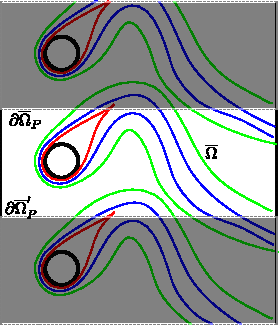
\includegraphics[width=0.4\linewidth]{periodic_bc.pdf}
\caption{Ячейка периодичности в задаче обтекания бесконечной решётки}
\label{fig:periodic_bc}
\end{figure}
На \figref{fig:periodic_bc} представлен пример области с выделенной ячейкой периодичности $\overline\Omega$ (незатенённая область).
Изолинии можно трактовать как изотермы решения задачи о нестационарном обтекании решётки нагревателя
(поле температур в этом случае описывается более сложным уравнением, чем \cref{eq:poissonnd_lam}
и приведено тут только для иллюстрации периодичности).

Пара периодических границ обозначена через $\partial\overline\Omega_P$ и $\partial\overline\Omega_P'$.
Пусть эти границы топологически экваивалентны, то есть для любой точки $\vec x\in\partial\overline\Omega_P$
cуществует взаимноодносзначная точка $\vec x'\in\partial\overline\Omega_P'$.
Для того, чтобы решение за этими границами точно соответствовало решению внутри ячейки периодичности необходимо
задать равенство значений и производных любого порядка:
\begin{equation}
\label{eq:poissonnd_bcp}
\left\{
\begin{array}{l}
    u(\vec x) = u(\vec x'), \\ [10pt]
    \left.\displaystyle\frac{\partial^k u}{\partial n^k}\right|_{\vec x} = -\left.\displaystyle\frac{\partial^k u}{\partial n^k}\right|_{\vec x'}
\end{array}
\right.
\vec x\in\partial\overline\Omega_P, \quad \vec x'\in\partial\overline\Omega_P', \quad \forall k.
\end{equation}
Здесь под $n$ подразумевается внешняя к ячейке периодичности нормаль, поэтому в правой части
условия для производных стоит минус.


\subsection{Метод конечных разностей}
\label{sec:poisson_fdm}
Будем рассмотривать задачу \cref{eq:poissonnd,eq:poissonnd_bc} в упрощённой одномерной постановке:
\begin{equation}
    \label{eq:poisson1d}
    -\ddfrq{u}{x} = f(x)
\end{equation}
в области $x\in[a,b]$.

Для аппроксимации производных методом конечных разностей будем использовать разложение Тейлора:
\begin{equation}
    \label{eq:taylor_series}
    u(x+h) = u(x) + h u'(x) + \frac{h^2}{2} u''(x) + \dots + \frac{h^{k}}{k!} u^{(k)}(x)
\end{equation}
из которой можно получить приближение первого (направленная разность) и второго (симметричная разность) порядков:
\begin{align}
    \label{eq:forwdiff}
    &u'(x) = \frac{u(x+h) - u(x)}{h} \underbrace{- \frac{h}{2}u''(x) - \frac{h^2}{6}u'''(x) - \dots}_{O(h)}, \\
    \label{eq:symdiff}
    &u'(x) = \frac{u(x+h/2) - u(x-h/2)}{h} \underbrace{-\frac{h^2}{24} u'''(x) - \frac{h^4}{1920} u^{(5)}(x) - \dots}_{O(h^2)}.
\end{align}

\subsubsection{Аппроксимация во внутренней области}

В области решения $[a,b]$ введём равномерную сетку из $N$ ячеек.
Шаг сетки будет равен $h=(b-a)/N$.
Узлы сетки запишем в виде сеточного вектора $\{x_i\}$ длины $N+1$, где $i=\overline{0,N}$.
Определим сеточный вектор $\{u_i\}$ неизвестных, элементы которого определяют значение искомого численного решения в $i$-ом узле сетки. 

Для аппроксимации оператора Лапласа из левой части исходного уравнения~\cref{eq:poisson1d} сначала
воспользуемся симметричной разностью~\cref{eq:symdiff} для снятия первой производной:
\begin{equation}
\label{eq:fdm_laplace_init}
u''(x) = \frac{u'(x+h/2) - u'(x-h/2)}{h} + O(h^2).
\end{equation}
Далее распишем первые производную с помощью той же формулы~\cref{eq:symdiff}:
\begin{align*}
& u'(x+h/2) = \frac{u(x+h) - u(x)}{h} - \frac{h^2}{24} u'''(x+h/2) + O(h^4)\\
& u'(x-h/2) = \frac{u(x) - u(x-h)}{h} - \frac{h^2}{24} u'''(x+h/2) + O(h^4).
\end{align*}
Запишем их разность, учитывая
\begin{equation*}
u'''(x+h/2) - u'''(x-h/2) = h u^{(4)}(x) + O(h^2).
\end{equation*}
Получим
\begin{equation*}
u'(x+h/2) - u'(x-h/2) = \frac{u(x+h) - 2 u(x) + u(x-h)}{h} - \frac{h^3}{24} u^{(4)}(x) + O(h^4).
\end{equation*}
Подставим последнее выражение в~\cref{eq:fdm_laplace_init}:
\begin{equation}
\label{eq:fdm_laplace_init}
u''(x) = -\frac{-u(x+h) + 2 u(x) - u(x-h)}{h^2} + O(h^2).
\end{equation}
Перенесём это выражение на равномерную сетку и окончательно запишем разностую схему второго порядка
для уравнения \cref{eq:poisson1d}
\begin{equation}
    \label{eq:poisson1d_fdm}
    \frac{-u_{i-1} + 2u_{i} - u_{i+1}}{h^2} = f_i, \qquad i=\overline{1,N-1}.
\end{equation}
Здесь $\{f_i\}$ -- известный сеточный вектор, определяемый через известную
аналитическую функцию $f(x)$ в правой части уравнения \cref{eq:poisson1d} как
\begin{equation}
    \label{eq:poisson1d_fdm2}
    f_i = f(x_i).
\end{equation}

\subsubsection{Сборка СЛАУ}
Линейные уравнения \cref{eq:poisson1d_fdm} относительно неизвестных $u_i$ составляют систему вида
\begin{equation*}
    \sum_{j=0}^{N} A_{ij}\,u_j = b_i, \qquad i=\overline{1,N-1}
\end{equation*}
с матричными коэффициентами
\begin{equation}
    \label{eq:poisson1d_fdm_lhs}
    A_{ij} = \begin{cases}
        2/h^2,  &\quad i=\overline{1,N-1}, \, j=i;\\
        -1/h^2, &\quad i=\overline{1,N-1}, \, j=i-1;\\
        -1/h^2, &\quad i=\overline{1,N-1}, \, j=i+1;\\
        0,      &\quad \text{иначе}.
    \end{cases}
\end{equation}
и правой частью
\begin{equation}
    \label{eq:poisson1d_fdm_rhs}
    b_i = f_i,   \quad i=\overline{1,N-1}.
\end{equation}
Всего в этой системе $N-1$ уравнение для $N+1$ неизвестной.
Для получения однозначного ответа не хватает двух уравнений, которые
должны быть сформулированы из граничных условий (для правой и левой границ).

\subsubsection{Учёт граничных условий}
\subsubsubsection{Граничные условия первого рода}

Рассмотрим условия первого рода вида:
\begin{equation}
	\label{eq:poisson1d_bc}
	\begin{cases}
        u(a)=u_a,\\[5pt]
        u(b)=u_b.\\
	\end{cases}
\end{equation}
Эти условия для сеточного вектора приобретут вид:
\begin{equation*}
u_0 = u_a, \qquad u_{N} = u_b.
\end{equation*}
В терминах матричных коэффициентов~\cref{eq:poisson1d_fdm_lhs,eq:poisson1d_fdm_rhs}
эти условия можно переписать в виде:
\begin{equation}
\begin{array}{ll}
A_{00} = 1, & b_{0} = u_a; \\
A_{NN} = 1, & b_{N} = u_b; \\
\end{array}
\end{equation}

\subsubsubsection{Граничные условия второго рода}
Рассмотрим условия Неймана
\begin{equation}
	\label{eq:poisson1d_bc2}
	\begin{cases}
        -\left.\ddfr{u}{n}\right|_a=q_a,\\[10pt]
        -\left.\ddfr{u}{n}\right|_b=q_b,
	\end{cases}
\end{equation}
Для их аппроксимации можно бы было воспользоваться направленными
разностями \cref{eq:forwdiff}. Учтём что нормаль $\vec n$ направлена наружу (против оси $x$ на левой границе и по оси $x$ -- на правой).
Тогда можно записать
\begin{equation}
- \frac{u_0 - u_1}{h} = q_a, \quad
- \frac{u_N - u_{N-1}}{h} = q_b,
\end{equation}
В терминах матричных коэффициентов получим
\begin{equation}
\label{eq:poisson1d_bc2_o1}
\begin{array}{lll}
A_{00} = 1/h & A_{01} = -1/h & b_0 = -q_a \\
A_{NN} = 1/h & A_{N,N-1} = -1/h & b_N = -q_b
\end{array}
\end{equation}

Следует однако заметить, что формула \cref{eq:forwdiff} имеет первый порядок
точности. Поэтому общий порядок расчётной схемы также будет первый.
Чтобы аппроксимировать граничные условия второго рода вторым порядком
воспользуемся уравнением \cref{eq:poisson1d_fdm} для
аппроксимации оператора Лапласа в граничной (левой) точке:
\begin{equation*}
u''_0 = \frac{u_{-1} - 2 u_{0} + u_{1}}{h^2}.
\end{equation*}
Здесь $u_{-1}$ -- это фиктивный узел, находящийся вне области расчёта.
Для нахождения его значения
аппроксимируем граничное условиe \cref{eq:poisson1d_bc2}
с использованием симметричной схемы \cref{eq:symdiff}:
\begin{equation*}
-\frac{u_{-1} - u_{1}}{2h} = q_a \hence
u_{-1} = u_{1} - 2 h q_a.
\end{equation*}
Используя два последних соотношения
запишем аппроксимированное уравнение Пуассона в граничной точке:
\begin{equation}
\label{eq:poisson1d_bc2left_o2}
-u''_0 = f_0 \hence
\frac{u_{0} - u_{1}}{h^2} = -\frac{q_a}{h} + \frac{1}{2} f_0.
\end{equation}
Переписывая в терминах матричных коэффициентов получим (сохраняя $h^2$ в знаменателе, чтобы
выражение имело тот же порядок, что и выражение для внутренних узлов \cref{eq:poisson1d_fdm}):
\begin{equation}
\label{eq:poisson1d_bc2_o2}
\begin{array}{lll}
A_{00} = 1/h^2 & A_{01} = -1/h^2 & b_0 = -\sfrac{q_a}{h} + \sfrac{f_0}{2} \\
A_{NN} = 1/h^2 & A_{N,N-1} = -1/h^2 & b_N = -\sfrac{q_b}{h} + \sfrac{f_N}{2}
\end{array}
\end{equation}
Ещё раз заметим, что все аппроксимационные формулы,
использованные для получения \cref{eq:poisson1d_bc2_o2}
имели второй порядок точности, поэтому
и само это выражение имеет второй порядок (в отличии от альтернативного \cref{eq:poisson1d_bc2_o1}).


\subsubsubsection{Граничные условия третьего рода}
Аппроксимацию условий третьего рода
\begin{equation}
	\label{eq:poisson1d_bc2}
	\begin{cases}
        -\left.\ddfr{u}{n}\right|_a=\alpha_a u(a) + \beta_a,\\[10pt]
        -\left.\ddfr{u}{n}\right|_b=\alpha_b u(b) + \beta_b,
	\end{cases}
\end{equation}
можно получить по аналогии с аппроксимацией
условий второго рода, заменив $q$ на $\alpha u + \beta$.
В частности, для левого узла
аппроксимация второго порядка по аналогии с \cref{eq:poisson1d_bc2left_o2}
примет вид
\begin{equation*}
\label{eq:poisson1d_bc3left_o2}
-u''_0 = \alpha_a u_0 + \beta \hence
\frac{(1 + \alpha_a h) u_{0} - u_{1}}{h^2} = -\frac{\beta}{h} + \frac{1}{2} f_0.
\end{equation*}
А на матричном уровне получим
\begin{equation}
\label{eq:poisson1d_bc3_o2}
\begin{array}{lll}
A_{00} = (1 + \alpha_a h)/h^2 & A_{01} = -1/h^2 & b_0 = -\sfrac{\beta_a}{h} + \sfrac{f_0}{2} \\
A_{NN} = (1 + \alpha_b h)/h^2 & A_{N,N-1} = -1/h^2 & b_N = -\sfrac{\beta_b}{h} + \sfrac{f_N}{2}
\end{array}
\end{equation}

\subsubsubsection{Периодические граничные условия}

Для удовлетворения периодических условий
можно на сеточном уровне 
закольцевать сетку, переименовав
узел с индексом ${N}$ в узел $0$, узел ${N+1}$ в $1$  и т.п.
В сеточном векторе тогда останется $N$ неизвестных.
Уравнения для крайних точек примут вид
\begin{equation}
    \label{eq:poisson1d_per0}
    \frac{-u_{N-1} + 2u_{0} - u_{1}}{h^2} = f_0, \qquad 
    \frac{-u_{N-2} + 2u_{N-1} - u_{0}}{h^2} = f_{N-1}.
\end{equation}

\subsubsection{Двумерная задача}
Двумерная задача Пуассона в частных производных будет иметь вид
\begin{equation}
    \label{eq:poisson_2d}
   -\left(\dfrq{u}{x} + \dfrq{u}{y}\right) = f(x, y).
\end{equation}

Разностную схему для такого уравнения удобно писать и использованием парного индекса $(i,j)$, где $i$ -- индекс вдоль оси $x$, $j$ -- индекс вдоль оси $y$.
При этом сеточные вектора должны по прежнему оставаться линейными массивами.
Функцию, переводящую парный индекс в сквозной (линейный), обозначим как
\begin{equation}
    \label{eq:poisson_fdm_2d_ij2k}
    k[i, j] = i + (n_x+1) j
\end{equation}
$n_x$ -- количество ячеек сетки в направлении x.
Обратные функции, переводящие сквозной индекс в пару $i,j$, имеют вид
\begin{equation}
    \label{eq:poisson_fdm_2d_k2ij}
    \begin{array}{ll}
        i[k] = {\rm mod}\left(k, \left(n_x+1\right)\right), & \text{// остаток от деления},\\
        j[k] = \lfloor k / \left(n_x+1\right)\rfloor,       &\text{// целая часть от деления}.\\
    \end{array}
\end{equation}

С учётом введённых обозначений разностная схема для уравнения \cref{eq:poisson_2d} примет вид
\begin{equation}
   \label{eq:poisson_fdm_2d}
   \frac{-u_{k[i-1,j]} + 2 u_{k[i, j]} - u_{k[i+1,j]}}{h_x^2} +
   \frac{-u_{k[i,j-1]} + 2 u_{k[i, j]} - u_{k[i,j+1]}}{h_y^2} =
   f_{k[i,j]},
\end{equation}

\subsubsection{Верификация порядка аппроксимации}
\label{sec:compute-appr}

Порядок аппрокцимации показывает скорость
приближения численного решения к точному с уменьшением сетки.
Поэтому для подтверждения порядка необходимо
\begin{itemize}
\item Знать точное решение,
\item Уметь вычислять функционал (норму, $||\cdot||$), характеризующий отклонение точного решения от численного,
\item Сделать несколько расчётов на сетках с разной $N$  и заполнить таблицу $||\{u_i - u^e(x_i)\}||(N)$,
\item На основе этой таблицы построить график в логарифмических осях и по углу наклона кривой сделать вывод о порядке аппроксимации.
\end{itemize}

Выберем произвольную функцию $u^e$ (достаточно сильно изменяющуюся на целевом отрезке $[a,b]$).

Далее путём прямого вычисления определим параметры задачи $f$, $u_a$, $u_b$ такие,
для которых функция $u^e$ является точным решением задачи \cref{eq:poisson1d}, \cref{eq:poisson1d_bc}.

Зададимся числом разбиений $N$ и решим задачу для выбранным параметров.
В результате определим сеточный вектор численного решения $\{u_i\}$.

В качестве нормы выберем стандартное отклонение. В интегральном виде для многомерной функции $y(\vec x)$
в области $\vec x\in D$ оно имеет вид
\begin{equation}
    \label{eq:norm2_common}
    ||y(\vec x)||_2 = \sqrt{\frac{1}{|D|}\int_{D} y(\vec x)^2 \, d\vec x}.
\end{equation}
Упрощая до одномерного случая
\begin{equation*}
    ||y(x)||_2 = \sqrt{\frac{1}{b-a}\int_{a}^{b} y(x)^2 \, dx}.
\end{equation*}

Вычислим этот интеграл численно на введённой ранее равномерной сетке $\{x_i\}$:
\begin{equation*}
    ||\{y_i\}||_2 = \sqrt{\frac{1}{b-a}\sum_{i=0}^{N} w_i y_i^2},
\end{equation*}
где $\{w_i\}$ -- вес (или "площадь влияния") $i$-ого узла:
\begin{equation*}
    w_i = \begin{cases}
        h/2, &\quad i=0, N;\\
        h, &\quad i=\overline{1,N-1},
    \end{cases}
\end{equation*}
такая что
\begin{equation*}
    \sum_{i=0}^{N} w_i = b-a.
\end{equation*}

Окончательно среднеквадратичная норма отклонения численного решения от точного запишется в виде
\begin{equation}
    \label{eq:poisson1d_fdm_norm}
    ||\{u_i - u^e(x_i)\}||_2 = \sqrt{\frac{1}{b-a}\sum_{i=0}^{N} w_i \left(u_i - u^e_i\right)^2}.
\end{equation}

Пример программы, реализующей этот алгоритм смотри в \secref{sec:poisson1d_prog}.

%\subsection{Метод конечных объёмов}
\label{sec:FVM}
Будем рассматривать задачу в многомерной постановке \cref{eq:poissonnd,eq:poissonnd_bc}.

\subsubsection{Конечнообъёмная сетка}
Разобъём oбласть численного решения на непересекающиеся подобласти $E_i$, $i = \overline{0, N-1}$,
а её границу $\partial \Omega$ на грани $\Gamma_s$, $s = \overline{0, N^\Gamma - 1}$ (\figref{fig:fvm_grid}).
Введем следующие сеточные примитивы:
\begin{itemize}
\item $E_i$ -- ячейка сетки,
\item $\Gamma_{s}$ -- граничная грань,
\item $\vec x_i$ -- центр (масс) ячейки,
\item $\vec g_s$ -- центр (масс) грани $\Gamma_{s}$,
\item $\gamma_{ij}$ -- внутренняя грань между $i$-ой и $j$-ой ячейками,
\end{itemize}
Будем считать, что ячейки сетки выпуклые, а грани -- плоские.

\begin{figure}[h!]
\centering
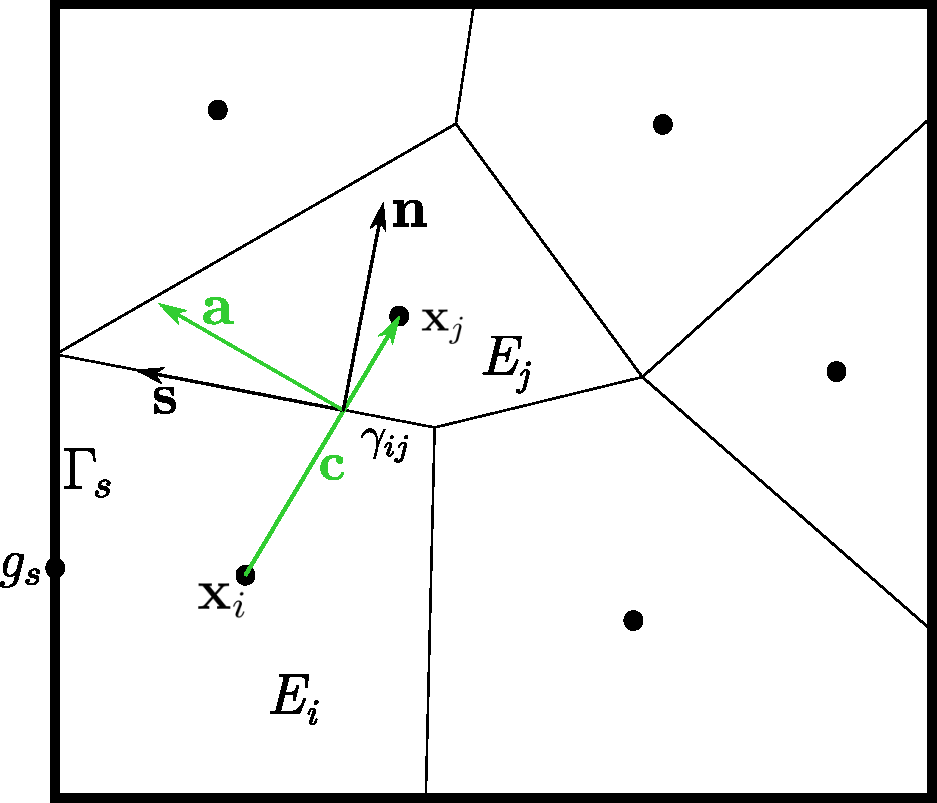
\includegraphics[width=0.4\linewidth]{fvm_grid.pdf}
\caption{Конечнообъёмная сетка}
\label{fig:fvm_grid}
\end{figure}

\subsubsection{Конечнообъёмная аппроксимация}
\label{sec:fvm_appr}

Проинтегрируем исходное уравнение по одной из подобластей $E_i$:
\begin{equation*}
-\arint{\nabla^2 u}{E_i}{s} = \arint{f}{E_i}{\vec x}.
\end{equation*}
К интегралу в левой части применим формулу интегрирования по частям \cref{eq:partint_laplace}. Получим
\begin{equation}
\label{eq:fvm_pois_int}
-\arint{\dfr{u}{n}}{\partial E_i}{\vec x} = \arint{f}{E_i}{\vec x}.
\end{equation}
Здесь $\partial E_i$ -- совокупность всех границ подобласти $E_i$,
а $\vec n$ -- внешняя к подобласти нормаль.

Граница ячейки $E_i$ состоит из внутренних граней $\gamma_{ij}$ (индекс $j$ здесь
соответствует индексу соседней ячейки)
и инцидентных ей граней $\Gamma_{s}$, лежащих на внешней границе расчётной области $\Omega$.
Тогда интеграл по общей границе ячейки распишется через сумму интегралов по плоским поверхностям
$$
\arint{\dfr{u}{n}}{\partial E_i}{s} = \sum_{j\in{{\rm J}_i}}\arint{\dfr{u}{n}}{\gamma_{ij}}{s} + \sum_{s\in{\rm I}_i, {\rm II}_i}\arint{\dfr{u}{n}}{\Gamma_{s}}{s}.
$$
Введены следующие обозначения множества индексов: ${\rm J}_i$ -- индексы ячеек, соседних (имеющих общую грань) с текущей ячейкой $i$,
${\rm I}_i, {\rm II}_i$ -- индексы граничных граней первого и второго рода, инцидентных ячейке $E_i$.
Аппроксимирум производную $\dsfr{u}{n}$ на каждой из граней константой.
Тогда её можно вынести из под интегралов и предыдущее выражение записать в виде
\begin{equation}
\label{eq:fvm_gamma_integral}
\arint{\dfr{u}{n}}{\partial E_i}{s} \approx
\sum_{j\in{{\rm J}_i}}
    \left|
        \gamma_{ij}
    \right|
    \left(
        \dfr{u}{n}
    \right)_{\gamma_{ij}}
+\sum_{s\in{{\rm I}_i, {\rm II}_i}}
    \left|
        \Gamma_{s}
    \right|
    \left(
        \dfr{u}{n}
    \right)_{\Gamma_{s}}
\end{equation}
Здесь $|\gamma_{ij}|$, $|\Gamma_s|$ -- площади граней.

Аналогично, анализируя интеграл правой части \cref{eq:fvm_pois_int},
приблизим значение функции правой части $f$ внутри элемента $E_i$ константой $f_i$,
которую отнесём к центру элемента. Тогда
\begin{equation}
\label{eq:fvm_f_integral}
\arint{f}{E_i}{\vec x} \approx f_i \left|E_i\right|.
\end{equation}

Сеточный вектор $\{f_i\}$ -- есть конечнообъёмная аппроксимация
функции $f(\vec x)$ на конечнообъёмную сетку.
Значения $f_i$ при аппроксимации чаще всего находятся как значения в центрах элементов
$$
f_i = f(\vec x_i).
$$
Хотя иногда может быть использовано и другое определение,
следующее из \eqref{eq:fvm_f_integral}:
$$
f_i = \frac{1}{\left| E_i \right|} \arint{f(\vec x)}{E_i}{\vec x}.
$$


\subsubsubsection{Обработка внутренних граней}
Для начала будем рассматривать сетки, в
которых вектора $\vec c$, соединяющие центры ячеек (зедёные вектора на \figref{fig:fvm_grid}),
коллинеарны (или почти коллинеарны) нормалям к граням $\vec n$.
В этом случае производную искомой функции по нормали к грани можно записать в виде
$$
\dfr{u}{n} = \dfr{u}{c}.
$$

Далее определим значения функции $u$ в точках $\vec x_i$, $\vec x_j$ как $u_i$, $u_j$.
Тогда значение производной $\dsfr{u}{n}$ на внутренней грани конечного объёма
может быть приближена конечной разностью
\begin{equation}
\label{eq:fvm_dudn_dudc}
\left(\dfr{u}{n}\right)_{\gamma_{ij}} \approx \dfr{u}{c} \approx \frac{u_j - u_i}{h_{ij}}, \quad h_{ij} = |\vec x_j - \vec x_i|.
\end{equation}

Определим pebi (perpendicular-bisector) сетки как сетки, удовлетворяющие следующим свойствам
\begin{itemize}
\item линии, соединяющие центры двух соседних ячеек, перпендикулярны грани между этими ячейками;
\item внутренние грани делят линии, соединящие центры соседних ячеек, пополам.
\end{itemize}
Очевидно, что равномерная структурированная сетка удовлетворяет этим свойствам.
Для построения неструктурированных pebi-сеток используют алгоритмы построения ячеек Вороного.
Для pebi-сеток разностная схема \eqref{eq:fvm_dudn_dudc}
является симметричной разностью и, поэтому, имеет второй порядок аппроксимации.

\subsubsubsection{Учёт граничных условий}
Для вычисления второго слагаемого в правой части 
\cref{eq:fvm_gamma_integral}
следует расписать значение нормальной 
к границе производной вида
$$
\left(\dfr{u}{n}\right)_{\Gamma_{s}}.
$$
Это делается с помощью граничных условий.

\paragraph{Условия первого рода}
Пусть в центре $\vec g_s$ грани $\Gamma_{s}$ задано 
значение искомой функции \cref{eq:poissonnd_bc}:
\begin{equation}
\label{eq:fvm_bc1}
u(\vec g_s) = u^\Gamma_s.
\end{equation}
Аппроксимацию производных
будем проводить из тех же соображений, которые использовали
при анализе внутренних граней. Только вместо центра соседнего элемента
$c_j$ будем использовать центр грани $g_s$.
В первом приближении, отбрасывая касательные производные, придём к формуле, аналогичной \cref{eq:fvm_dudn_dudc}:
\begin{equation}
\label{eq:fvm_bc1_approx}
\left(\dfr{u}{n}\right)_{\Gamma_s} \approx \frac{u^\Gamma_s - u_i}{h^\Gamma_{is}}, \quad h^\Gamma_{is} = \left| \vec g_s  - \vec x_i \right|.
\end{equation}

\paragraph{Условия второго рода}
В условиях второго рода нормальная производная уже задана явно:
\begin{equation*}
\left(\dfr{u}{n}\right)_{\Gamma_s} = -q_s.
\end{equation*}

\subsubsection{Одномерный случай}
Рассмотрим результат конечнообъёмной аппроксимации
задачи \cref{eq:poissonnd} в одномерном случае \cref{eq:poisson1d}
на равномерной сетке с шагом $h$ (\figref{fig:fvm_grid1d}).

\begin{figure}[h!]
\centering
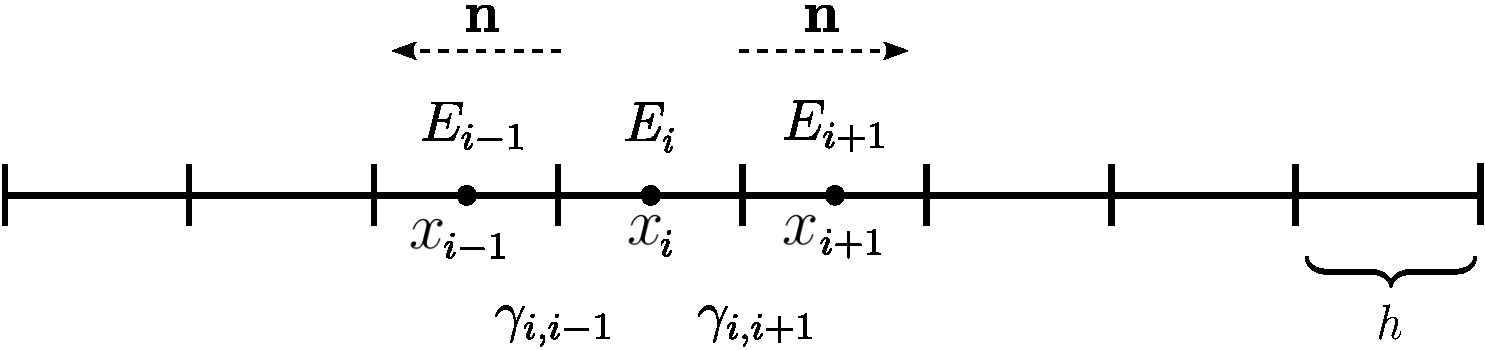
\includegraphics[width=0.6\linewidth]{fvm_grid1d.pdf}
\caption{Одномерная конечнообъёмная сетка}
\label{fig:fvm_grid1d}
\end{figure}

У внутренней ячейки $i$ есть две границы: $\gamma_{i,i-1}$ и $\gamma_{i,i+1}$.
Нормали по этим границам аппроксимируются по формулам \cref{eq:fvm_dudn_dudc}:
\begin{align*}
\gamma_{i,i-1}: \quad& \dfr{u}{n} = \frac{u_{i-1}-u_{i}}{h} \\[10pt]
\gamma_{i,i+1}: \quad& \dfr{u}{n} = \frac{u_{i+1}-u_{i}}{h}
\end{align*}
Объём ячейки в одномерном случае равен её длине $h$.
Площадь грани следует положить единице с тем, чтобы
$$
|E_i| = |\gamma| h = h.
$$
Тогда, подставляя эти значения в \cref{eq:fvm_pois_int},
получим знакомую конечноразностную схему аппроксимацию уравнения Пуассона
$$
\frac{-u_{i-1} + 2 u_i - u_{i+1}}{h} = f_i h,
$$
которая имеет второй порядок точности.

Разница со схемой, полученной  методом конечных разностей \cref{eq:poisson1d_fdm}, здесь состоит в том,
что значения сеточных векторов $\gvec{u}$, $\gvec{f}$ здесь
приписаны к центрам ячеек, а не к их вершинам.
Это отличие проявит себя в аппроксимации граничных условий.
Так, если на левой границе $x=a$ задано условие первого рода, то соответствующее уравнение
согласно \cref{eq:fvm_bc1_approx}
примет вид
$$
-\frac{u^\Gamma_a - u_0}{h/2} - \frac{u_1 - u_0}{h} = f_0 h.
$$
В методе конечных разностей это условие выразилось бы в виде $u_0 = u^\Gamma_a$.

\subsubsection{Сборка системы линейных уравнений}
Подставим все полученные аппроксимации
\cref{eq:fvm_dudn_dudc,eq:fvm_bc1_approx}
в уравнение \cref{eq:fvm_pois_int}. Получим $i$-ое уравнение искомой системы уравнений относительно неизвестных $u_i$:
\begin{equation*}
-\sum_{j\in {\rm J}_i}
    \frac{|\gamma_{ij}|}{h_{ij}}
         \left(u_j - u_i\right)
-\sum_{s\in{\rm I}_i}
    \frac{|\Gamma_{s}|}{h^\Gamma_{is}}
        \left(u^\Gamma_s - u_i\right)
+\sum_{s\in{\rm II}_i} q_s |\Gamma_s|
=
f_i |E_i|.
\end{equation*}
Здесь первое слагаемое в левой части отвечает за потоки через внутренние границы,
второе -- граничные условия первого рода.
Далее перенесём все известные значения в правую часть и окончательно
получим линейное уравнение для $i$-го конечного объёма:
\begin{equation}
\label{eq:fvm_slae}
\sum_{j\in{\rm J}_i}
    \frac{|\gamma_{ij}|}{h_{ij}}
         \left(u_i - u_j\right)
+\sum_{s\in{\rm I}_i}
    \frac{|\Gamma_{s}|}{h^\Gamma_{is}}u_i
 =
f_i |E_i|
+\sum_{s\in{\rm I}_i}
    \frac{|\Gamma_{s}|}{h^\Gamma_{is}} u_s^\Gamma
-\sum_{s\in{\rm II}_i} q_s |\Gamma_{s}|.
\end{equation}
Таким образом мы получили систему из $N$ (по количеству подобластей) линейных уравнений относительно
неизвестного сеточного вектора $\left\{u_i\right\}$
$$
A u = b.
$$

Полученные в результате сборочных процедур матрицы являются разреженными -- то есть большинство их элементов равно нулю.
Полное хранение таких матриц в памяти невозможно, поэтому применяют специальные процедуры разреженного хранения (см. \secref{sec:sparse-matrix}).

Ниже приведён псеводкод для сборки СЛАУ. Перед началом процедур сборки левую правую часть нужно инициализировать нулями.

\subsubsubsection{Алгоритм сборки в цикле по ячейкам}
\label{sec:poisson_fvm_cellbased}
Матрицу $A$ и правую часть $b$ системы \cref{eq:fvm_slae} можно
собирать в цикле по ячейкам: строчка за строчкой.
Такой алгоритм выглядел бы следующим образом
\begin{equation*}
\begin{array}{ll}
\textbf{for } i = \overline{0, N-1}                          & \textrm{-- цикл по строкам СЛАУ}\\
\qquad b_i = |E_i| f_i                                       & \\
\qquad \textbf{for } j \in \textrm{nei(i)}                   & \textrm{-- цикл по ячейкам, соседним с ячейкой $i$}\\
\qquad \qquad v = \sfrac{|\gamma_{ij}|}{h_{ij}}              & \\
\qquad \qquad A_{ii} \pluseq v                               & \\
\qquad \qquad A_{ij} \minuseq v                              & \\
\qquad \textbf{endfor}                                       & \\
\qquad \textbf{for } s \in \textrm{bnd1(i)}                  & \textrm{-- цикл по граням ячейки $i$ с условиями первого рода}\\
\qquad \qquad v = \sfrac{|\Gamma_{s}|}{h^\Gamma_{is}}        & \\
\qquad \qquad A_{ii} \pluseq v                               & \\
\qquad \qquad b_{i}  \pluseq u_s^{\Gamma} v                  & \\
\qquad \textbf{endfor}                                       & \\
\qquad \textbf{for } s \in \textrm{bnd2(i)}                  & \textrm{-- цикл по граням ячейки $i$ с условиями второго рода}\\
\qquad \qquad b_{i}  \minuseq q_s |\Gamma_s|                  & \\
\qquad \textbf{endfor}                                       & \\
\textbf{endfor}
\end{array}
\end{equation*}
Первым недостатком такого алгоритма является наличие вложенных циклов.
Во-вторых, коэффициент, отвечающий за поток через внутреннюю грань $\gamma_{ij}$,
равный $\sfrac{|\gamma_{ij}|}{h_{ij}}$ в таком алгоритме будет учитываться дважды:
в строке $i$ и в строке $j$.

\subsubsubsection{Алгоритм сборки в цикле по граням}
\label{sec:poisson_fvm_facebased}
Вместо общего цикла по ячейкам, будем использовать цикл по граням.
В таком цикле коэффициенты потоков будут вычисляться один раз
и вставляться сразу в две строки матрицы, соответствующие соседним с гранью ячейкам.
Вложенных циклов в такой постановке удаётся избежать, потому
что у грани есть только две соседние ячейки (в то время как у ячейки может быть произвольное
количество соседних граней).

Разделим все грани на исходной сетки на внутренние и граничные (отдельный набор для каждого вида граничных условий).
Тогда для внутренних граней можно записать
\begin{equation}
\label{eq:fvm_assem_internal}
\begin{array}{ll}
\textbf{for } s \in\textrm{internal}                     & \textrm{-- цикл по внутренним граням}\\ 
\qquad i,j = \textrm{nei\_cells(s)}                      & \textrm{-- две ячейки, соседние с текущей гранью}\\
\qquad v = \sfrac{|\gamma_{ij}|}{h_{ij}}                 & \\
\qquad A_{ii} \pluseq  v; \quad A_{jj} \pluseq  v        & \textrm{-- диагональные коэффициенты матрицы}\\ 
\qquad A_{ij} \minuseq v; \quad A_{ji} \minuseq v        & \textrm{-- внедиагональные коэффициенты матрицы}\\
\textbf{endfor}                                          & \\
\end{array}
\end{equation}
Граничные условия учитываются в отдельных циклах.
Здесь будем учитывать, что у грани, принадлежащей
границе области, есть только одна соседняя ячейка:
\begin{equation}
\label{eq:fvm_assem_bc1}
\begin{array}{ll}
\textbf{for } s \in\textrm{bnd1}                         & \textrm{-- грани с условиями первого рода}\\ 
\qquad i = \textrm{nei\_cell(s)}                         & \textrm{-- соседняя с граничной гранью ячейка}\\
\qquad v = \sfrac{|\Gamma_{s}|}{h^\Gamma_{is}}           & \\
\qquad A_{ii} \pluseq  v                                 & \\ 
\qquad b_{i} \pluseq u_s^\Gamma v                        & \\
\textbf{endfor}                                          & \\
\textbf{for } s \in\textrm{bnd2}                         & \textrm{-- грани с условиями второго рода}\\ 
\qquad i = \textrm{nei\_cell(s)}                         & \textrm{-- соседняя с граничной гранью ячейка}\\
\qquad b_{i} \minuseq q_s |\Gamma_s|                     & \\
\textbf{endfor}                                          & \\
\end{array}
\end{equation}
Первое слагаемое в правой части
\cref{eq:fvm_slae}
учтём отдельным циклом:
\begin{equation}
\label{eq:fvm_assem_f}
\begin{array}{ll}                                         & \\
\textbf{for } i = \overline{0,N-1}                        & \textrm{-- цикл по ячейкам}\\ 
\qquad b_i \pluseq |E_i| f_i                              & \\
\textbf{endfor}                                           &
\end{array}
\end{equation}

\subsubsection{Расширенный набор точек коллокаций}
\label{sec:poisson_fvm_extended_facebased}
До сих пор мы соотносили
элементы сеточных векторов, которые получаются при аппроксимации функции на конечнообъёмную сетку,
с центрами конечных объёмов.
То есть точками коллокации служили центры объёмов,
а длина сеточных векторов (количество точек коллокации)
равнялась количеству ячеек сетки.
Для написания аппроксимационных соотношений около границ будет удобно расширить набор точек коллокаций за счёт
центров граничных граней.
Тогда у каждой грани будет две иницидентные точки коллокации: у внутренних граней -- это
центры инцидентных ячеек, у граничных -- это центр иницидентной ячейки и центр самой грани.

Такой подход позволяет универсализировать подходы
к аппроксимации перетоков через грани.
То есть для каждой грани вмеcто использования разных алгоритмов для внутренних \cref{eq:fvm_assem_internal} и граничных \cref{eq:fvm_assem_bc1} граней, нужно использовать универсальный алгоритм
\begin{equation}
\label{eq:fvm_assem_bc_extended}
\begin{array}{ll}
\textbf{for } s \in\overline{0, N_f - 1}            & \textrm{-- цикл по всем граням}\\
\qquad i,j = \textrm{nei\_colloc(s)}                & \textrm{-- инцидентные точки коллокаций}\\
\qquad v = \sfrac{|\gamma_{ij}|}{h_{ij}}            & \\
\qquad A_{ii} \pluseq  v, \quad A_{ij} \minuseq v   & \textrm{-- $i$-ая строка}\\ 
\qquad A_{jj} \pluseq  v, \quad A_{ji} \minuseq v   & \textrm{-- $j$-ая строка}\\ 
\textbf{endfor}                                     & \\
\end{array}
\end{equation}
Отметим, что эта процедура заполняет не только строки, соответствующие внутренним коллокациям, но и строки для граничных точек.
Последние заполняются выражениями, соответствующие интегралам от нормальных производных
\begin{equation*}
-\arint{\dfr{u}{n}}{\Gamma_s}{s} \approx -\left.\dfr{u}{n}\right|_{\vec{g}_s} |\Gamma_s|\
\approx \frac{u^\Gamma_s - u_j}{h^\Gamma_{is}} |\Gamma_s|,
\end{equation*}
где $i$ -- индекс ячейки, соседний с гранью $\Gamma_s$.
Для задач с граничными условиями первого рода эти строки излишни и будут переписаны, но они окажутся
полезными позднее, при учёте других типов граничных условий.

Строки матрицы, соответствующие граничным точкам коллокации,
будут содержеть аппроксимированные граничные условия.
Так, для граней с условиями первого рода будет аппроксимироваться непосредственно выражение
\cref{eq:fvm_bc1}. Алгоритмическом виде это примет вид
\begin{equation}
\label{eq:fvm_assem_bc1_extended}
\begin{array}{ll}
\textbf{for } s \in\textrm{bnd1}                         & \textrm{-- грани с условиями первого рода}\\ 
\qquad j = \textrm{bnd\_col(s)}                          & \textrm{-- индекс точки коллокации, соответствующей грани}\\
\qquad A_{ij} = \delta_{ij}                              & \textrm{-- единичная диагональ}\\ 
\qquad b_{j} = u^\Gamma_s                                & \\
\textbf{endfor}                                          & \\
\end{array}
\end{equation}

Преимуществами такого подхода является:
\begin{itemize}
\item Более очевидный учёт граничных условий в отдельной строке СЛАУ,
\item Наличие явно выраженного граничного значения функции в сеточном векторе.
\end{itemize}

\subsubsubsection{Пример}
\begin{figure}[h]
\centering
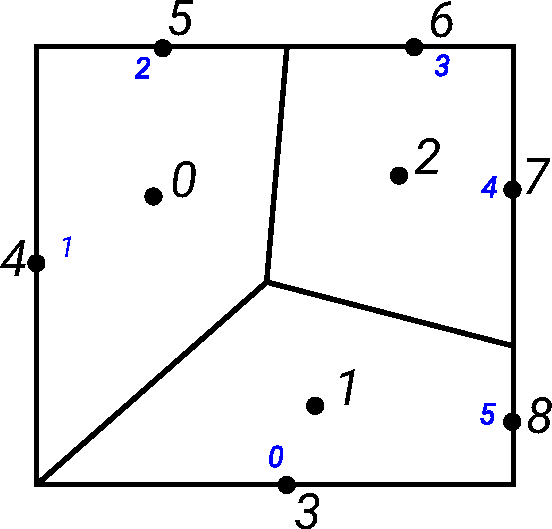
\includegraphics[width=0.25\linewidth]{extended_coll.pdf}
\caption{Расширенный набор точек коллокации}
\label{fig:extended_coll}
\end{figure}

На рис.~\ref{fig:extended_coll}.
представлена конечнообъёмная сетка, содержащая три ячейки
и девять граней. Индексация граничных граней обозначена синими цифрами.
Согласно стандартной методике конечных
объёмов сеточная функция
будет представлена массивом из трёх элементов.
В расширенном наборе будет девять точек коллокации (обозначены чёрными кругами и проиндексированы чёрными цифрами):
три соответствуют центрам ячеек и ещё шесть -- центрам граничных граней.

Пусть в области с рис.~\ref{fig:extended_coll} нужно решить
уравнение Пуассона \cref{eq:poissonnd}.
Пусть на нижней и правой гранях задано условие первого рода: $u = C$.

\paragraph{Классический подход}
Согласно классическому методу конечных объёмов
(\secref{sec:poisson_fvm_facebased})
аппроксимация задачи в ячейке с индексом 1 будет иметь следующий вид
$$
\frac{u_1 - u_0}{h_{10}}|\gamma_{10}|
+\frac{u_1 - u_2}{h_{12}}|\gamma_{12}|
+\frac{u_1 - C}{h^\Gamma_{10}}|\Gamma_0|
+\frac{u_1 - C}{h^\Gamma_{15}}|\Gamma_5|
= |E_1| f_1.
$$
Общая размерность матрицы СЛАУ при таком подходе будет
равна $3\times3$, а её элементы в 1-ой строке равны
$$
a_{10} = -\frac{|\gamma_{10}|}{h_{10}},  \quad
a_{12} = -\frac{|\gamma_{12}|}{h_{12}},  \quad
a_{11} = \frac{|\gamma_{10}|}{h_{10}}  + \frac{|\gamma_{12}|}{h_{12}} + \frac{|\Gamma_{0}|}{h^\Gamma_{10}} + \frac{|\Gamma_5|}{h^\Gamma_{15}}.
$$
Справа в 1-ой строке будет стоять
$$
b_1 = |E_1| f_1 + \frac{C |\Gamma_0|}{h^\Gamma_{10}} + \frac{C |\Gamma_5|}{h^\Gamma_{15}}.
$$

\paragraph{Расширенный набор точек коллокаций}
Здесь матрица правой части будет иметь размерность $9\times9$.
Из них первые три будут собираться согласно классической процедуре
метода конечных объёмов, но учитывая наличие дополнитиельных точек коллокации в центрах
граничных граней. Так, 1-ое уравнение итоговой СЛАУ, собранной согласно процедуре из
\secref{sec:poisson_fvm_extended_facebased},
примет вид
$$
\frac{u_1 - u_0}{h_{10}}|\gamma_{10}|
+\frac{u_1 - u_2}{h_{12}}|\gamma_{12}|
+\frac{u_1 - u_3}{h_{13}}|\gamma_{13}|
+\frac{u_1 - u_8}{h_{18}}|\gamma_{18}|
= |E_1| f_1.
$$
Здесь введено соотвествие для граничных граней и расстояний:
$$
\gamma_{13} = \Gamma_0, h_{13} = h^\Gamma_{10}, \gamma_{18} = \Gamma_5, h_{18} = h^\Gamma_{15}.
$$
Остальные шесть уравнений будут представлять из себя
аппроксимацию граничных условий для соответствующих граней.
Так, 3-е и 8-е уравнение будет соответствовать условию первого рода:
$$
u_3 = C, \qquad u_8 = C.
$$
Переводя рассмотренные уравнения в матричные коэффициенты, получим
следующие ненулевые коээфиициенты итоговой матрицы $\{a_{ij}\}$ и вектора правой части $\{b_i\}$. Для 1-ой строки
$$
a_{10} = -\frac{|\gamma_{10}|}{h_{10}},  \quad
a_{12} = -\frac{|\gamma_{12}|}{h_{12}},  \quad
a_{13} = -\frac{|\gamma_{13}|}{h_{13}},  \quad
a_{18} = -\frac{|\gamma_{18}|}{h_{18}},  \quad
a_{11} = a_{10} + a_{12} + a_{13} + a_{18}, \quad
b_1 = |E_1| f_1,
$$
для 3-ей строки
$$
a_{33} = 1, \quad b_3 = C,
$$
для 8-ой строки
$$
a_{88} = 1, \quad b_8 = C.
$$

\subsubsubsection{Граничные условия второго рода}
Рассмотрим участок границы $\partial\Omega_{II}$ на котором заданы условия второго рода
\cref{eq:poissonnd_bc2} при $\lambda=1$.
Проинтегрируем это условие по грани и получим уравнение для граничного узла коллокации:
\begin{equation*}
-\arint{\dfr{u}{n}}{\Gamma_s}{s} = \arint{q(s)}{\Gamma_s}{s} \approx |\Gamma_s| q(\vec g_s).
\end{equation*}
При сборке матрицы левой части согласно процедуре
\cref{eq:fvm_assem_bc_extended} левая часть этого уравнения уже содержит
интеграл от нормальной производной.
Тогда алгоритм сборки этого условия будет включать в себя только подстановку $q$ в правую часть:
\begin{equation}
\label{eq:fvm_assem_bc2_extended}
\begin{array}{ll}
\textbf{for } s \in\textrm{bnd2}                         & \textrm{-- грани с условиями второго рода}\\ 
\qquad j = \textrm{bnd\_col(s)}                          & \textrm{-- индекс точки коллокации, соответствующей грани}\\
\qquad b_{j} = |\Gamma_s| q(\vec g_s)                    & \\
\textbf{endfor}                                          & \\
\end{array}
\end{equation}

\subsubsubsection{Граничные условия третьего рода}
Теперь рассмотрим участок границы $\partial\Omega_{III}$ с условиями
\cref{eq:poissonnd_bc3} при $\lambda=1$.
Так же проинтегрируем его по $s$-ой грани
\begin{equation*}
-\arint{\dfr{u}{n}}{\Gamma_s}{s} = \arint{\alpha(s) u + \beta(s)}{\Gamma_s}{s} \approx |\Gamma_s| \left(\alpha(\vec g_s) u_s + \beta(\vec g_s)\right).
\end{equation*}
Перенесём слагаемое с неизвестной $u_s$ в левую часть (то есть добавим коэффициент в диагональ матрицы), а $\beta$ оставим справа.
Тогда, после сборки матрицы левой части по процедуре 
\cref{eq:fvm_assem_bc_extended}, модифицируем матрицу и правую часть следующим образом:
\begin{equation}
\label{eq:fvm_assem_bc3_extended}
\begin{array}{ll}
\textbf{for } s \in\textrm{bnd3}                         & \textrm{-- грани с условиями третьего рода}\\ 
\qquad j = \textrm{bnd\_col(s)}                          & \textrm{-- индекс точки коллокации, соответствующей грани}\\
\qquad A_{jj} \pluseq |\Gamma_s| \alpha(\vec g_s)             & \\
\qquad b_{j} = |\Gamma_s| \beta(\vec g_s)                & \\
\textbf{endfor}                                          & \\
\end{array}
\end{equation}

\subsubsubsection{Периодические граничные условия}
\label{sec:periodic_fvm}
Рассмотрим периодическую пару границ $\partial\Omega_{P}$, $\partial\Omega_{P}'$.
Для того, чтобы такое условие можно было аппроксимировать сеточным методом,
необходимо, чтобы сетка на границе $\partial\Omega_P$ в точности соотвествовала сетке на границе $\partial\Omega_P'$.

Естественный способ удовлетворить граничные уловия вида
\cref{eq:poissonnd_bcp} -- модифицировать таблицы связности сетки так, чтобы грани, лежащие на этих границах перестали быть граничными.
То есть нужно убрать граничные точки коллокации, и добавить запись в таблицы связности \quo{грань-ячейка}.
Такая процедура требует специальной подстройки сеточных таблиц.

Чтобы этого избежать, можно работать без модификации сетки, но удовлетвормить формальным математическим условиям \cref{eq:poissonnd_bcp}.
Поскольку конечнообъёмная аппроксимация уравнения Пуассона имеет не более чем второй порядок точности, достаточно записать это условие только для первой производной.
Для периодической пары граничных граней с индексами $s$ и $s'$ это условие можно записать следующим образом:
\begin{align}
\label{eq:periodic_for_fem_poisson_1}
&u(\vec g_s) - u(\vec g_{s'}) = 0, \\
\label{eq:periodic_for_fem_poisson_2}
&-\arint{\dfr{u}{n}}{\Gamma_s}{s} - \arint{\dfr{u}{n}}{\Gamma_{s'}}{s} = 0.
\end{align}

Первое из этих условий условий запишем в строке, соответствующей грани $s$, а второе - в строке для грани $s'$.
При сборке \cref{eq:periodic_for_fem_poisson_2} учтём, что предворительно проведённая процедура
\cref{eq:fvm_assem_bc_extended}
собирает входящие в него пару интегралов в строках для грани $s$ и $s'$ соответсвенно.
Чтобы записать сумму этих интегралов, нужно просто суммировать эти строки матрицы.
Тогда процедура примет следующий вид

\begin{equation}
\label{eq:fvm_assem_bcp_extended}
\begin{array}{ll}
\textbf{for } s,s' \in\textrm{periodic\_pairs}           & \textrm{-- периодические пары граней}\\ 
\qquad i,j = \textrm{bnd\_col(s, s')}                    & \textrm{-- индексы граничных точек коллокации}\\
\qquad \textbf{for } k \in \overline{0, N+N^\Gamma-1}    & \textrm{-- цикл по столбцам}\\
\qquad\qquad  A_{jk} \pluseq A_{ik}                      & \textrm{-- складываем строки $i+j$ \cref{eq:periodic_for_fem_poisson_1}}\\
\qquad\qquad A_{ik} = 0                                  & \textrm{-- зануляем строку $i$}\\
\qquad \textbf{endfor}                                   & \\
\qquad A_{jj} \pluseq A_{ji}, \quad A_{ji} = 0           & \textrm{-- усилим диагональ $A_{jj}$ (т.к $u_i = u_j$)}\\
\qquad A_{ii} = 1, \quad A_{ij} = -1                     & \textrm{-- удовлетворим \cref{eq:periodic_for_fem_poisson_2}}\\
\textbf{endfor}                                          & \\
\end{array}
\end{equation}

\subsubsection{Учёт неортогональности сетки}
\label{sec:nonortho_fvm}
Конечнообъёмная схема, описываемая уравнениями \cref{eq:fvm_pois_int,eq:fvm_gamma_integral},
не использует в своем выводе аппроксимационных соотношений, и поэтому является точной.
Погрешность аппроксимации вносится при расписывании нормальных производных на грани
по разностным формулам: \cref{eq:fvm_dudn_dudc,eq:fvm_bc1_approx} через значения скалярной функции в точках коллокации.
Эти формулы имеют второй порядок аппроксимации в случае
ортогональных сеток. Поэтому для таких сеток
вся конечнообъёмная схема имеет второй порядок аппроксимации.
Но если в сетке присутствуют скошенные ячейки,
такие разностные соотношения дают только первый порядок точности.
Чтобы сохранить второй порядок для скошенных сеток необходимо 
дополнительно учитывать изменения функции поперёк нормали.

\begin{figure}[h!]
\centering
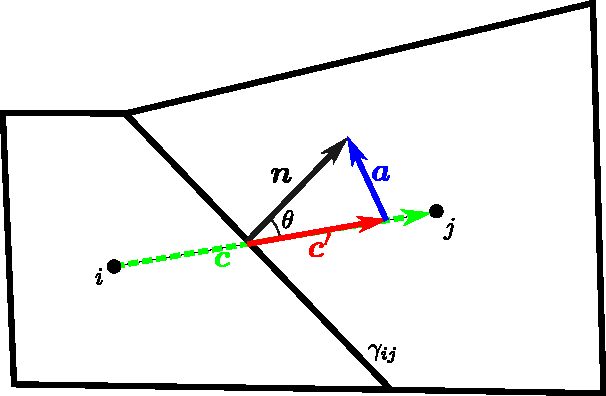
\includegraphics[width=0.4\linewidth]{skew_dfdn.pdf}
\caption{Ячейка периодичности в задаче обтекания бесконечной решётки}
\label{fig:skew_dfdn}
\end{figure}
Рассмотрим вычисление нормальной производной на грани $\gamma_{ij}$,
разделяющие точки коллокации $i$ и $j$ (\figref{fig:skew_dfdn}).
При использовании подхода с расширенным набором точек коллокации
не имеет значения, являются ли эти точки граничными коллокациями или внутренними.
Пусть вектор $\vec c$ соединяет точки коллокации.
За меру ортогональности примем значение угла $\theta$ 
между вектором единичной нормали $\vec n$ и вектором $\vec c$:
\begin{equation*}
\cos\theta = \frac{\vec n \cdot \vec c}{|\vec c|}.
\end{equation*}

Выделим некоторый вектор $\vec c'$, коллинеарный вектору $\vec c$.
И распишем вектор нормали как 
\begin{equation}
\label{eq:n_cprime_a}
\vec n = \vec c' + \vec a.
\end{equation}
Тогда
\begin{equation}
\label{eq:dudn_decomp}
\dfr{u}{n} = \nabla u \cdot \vec n = \nabla u \cdot \vec c' + \nabla u \cdot \vec a
= |\vec c'| \nabla u \cdot \frac{\vec c}{|\vec c|} + \nabla u \cdot \vec a.
\end{equation}
Первое слагаемое -- ортогональное приближение, которое 
с точностью до множителя $|\vec c'|$ равно ранее вычисленным
по разностным формулам \cref{eq:fvm_dudn_dudc,eq:fvm_bc1_approx}.
Второе -- поправка на скошенность.

Для реализации алгоритма с учётом этой поправки нужно решить следующие подзадачи:
\begin{itemize}
\item Задать длину $|\vec c'|$ (\secref{sec:cprime_a}),
\item Задать способ определения касательной производной $\nabla u\cdot \vec a$ (\secref{sec:fvm_duda}),
\item Собрать полученные соотношения в результирующую систему уравнений (\secref{sec:ortho_correction_assembly}).
\end{itemize}

\subsubsubsection{Методы разложения нормали}
\label{sec:cprime_a}
Рассмотрим различные варианты записи единичной нормали $\vec n$ в форме \cref{eq:n_cprime_a}.
Вектор $\vec c'$ сонаправлен заданному вектору $\vec c$, а вектор $\vec a$ может быть получен после определения $\vec c'$:
\begin{align*}
&\vec c' = |\vec c'| \frac{\vec c}{|\vec c|},\\
&\vec a = \vec n - \vec c'.
\end{align*}
То есть для конкретизации разложения  \cref{eq:n_cprime_a} нужно задать длину вектора $\vec c'$.
Рассмотрим три варианта её определения.

\paragraph{Поворот}

\begin{figure}[h!]
\centering
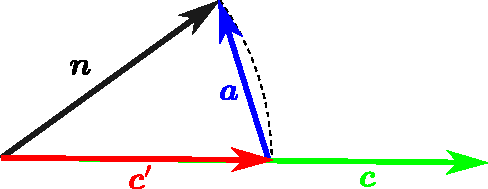
\includegraphics[width=0.4\linewidth]{cprime1.pdf}
\caption{Определение $\vec c'$ методом поворота}
\label{fig:cprime1}
\end{figure}

Положим $|\vec c'| = 1$. То есть положим длину искомого вектора равной длине единичной нормали $\vec n$ или повернём нормаль на угол $\theta$ (см. \figref{fig:cprime1}).
\begin{equation*}
\vec c' =  \frac{\vec c}{|\vec c|}.
\end{equation*}

\paragraph{Проекция}

\begin{figure}[h!]
\centering
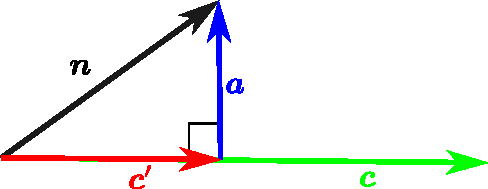
\includegraphics[width=0.4\linewidth]{cprime2.pdf}
\caption{Определение $\vec c'$ методом проекции}
\label{fig:cprime2}
\end{figure}

Определим вектор $\vec c'$ как проекцию вектора нормали на направление $\vec c$ (см. \figref{fig:cprime2}). Тогда
\begin{align*}
&|\vec c'| = \cos\theta = \frac{\vec n \cdot \vec c}{|\vec c|}, \\
&\vec c' = \frac{\vec n \cdot \vec c}{|\vec c|^2} \vec c
\end{align*}

В этом случае $|\vec c'| \leq 1$.
Таким образом, при записи нормальной производной \cref{eq:dudn_decomp} слагаемое с ортогональным приближением используется с коэффициентом, меньшим единицы.
Поэтому этот метод можно назвать методом нижней релаксации.

\paragraph{Обратная проекция}

\begin{figure}[h!]
\centering
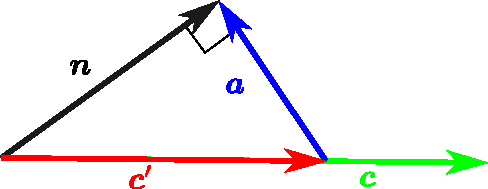
\includegraphics[width=0.4\linewidth]{cprime3.pdf}
\caption{Определение $\vec c'$ через обратную проекцию}
\label{fig:cprime3}
\end{figure}

Наоборот, опустим перпендикуляр с направления $\vec c$ на нормаль (см. \figref{fig:cprime3}):
\begin{align*}
&|\vec c'| = \frac{1}{\cos\theta} = \frac{|\vec c|}{\vec n \cdot \vec c}, \\
&\vec c' = \frac{\vec c}{\vec n \cdot \vec c}.
\end{align*}

Тогда, напротив $|\vec c'| \geq 1$, поэтому этот метод можно назвать методом верхней релаксации.
Отметим, что в этом случае вектор $\vec a$ будет параллелен грани $\gamma_{ij}$.

\subsubsubsection{Методы вычисления касательной производной}
\label{sec:fvm_duda}
Рассмотрим способы получить второе слагаемое из разложения \cref{eq:dudn_decomp}.
Напомним, что это разложение записывается для значения производной на грани конечноэлементной сетки:
\begin{equation*}
\left(\nabla u \cdot \vec a\right)_{\gamma_{ij}}
\end{equation*}
При этом функция $u$ задана своими значениями в точках коллокации, а вектор $\vec a$ известен (см. \secref{sec:cprime_a})

\paragraph{Определение через значение градиента в точках коллокации}
Пусть градиент $\nabla u$ также задан в точках коллокации.
Тогда значение на грани $\gamma_{ij}$ 
можно записать через линейную коминацию этих значений:
\begin{equation*}
\left(\nabla u\right)_{\gamma_{ij}} \approx w_i \left(\nabla u\right)_i + w_j \left(\nabla u\right)_j, \qquad w_i + w_j = 1.
\end{equation*}

Пусть $i$-ая точка коллокации граничная, тогда $w_i = 1, w_j = 0$.
Если же обе точки внутренние, то в простейшем случае можно взять $w_i = w_j = 0.5$.
В более сложных случаях можно подобрать весовые коэффициенты в зависимости от расстояние точки коллокации до грани.

Для определения градиента в точках коллокации применим алгорим опрелеления 
градинетов в центрах ячеек (см. \secref{sec:gradu_in_cells}).
К граничным точкам коллокации припишем значение градиента
из инцидентной с ней ячейкой.

Таким образом, пусть известны значение $(\nabla u)_i$ во внутренних точках коллокации. Тогда
значение градиента на границе будет равно
\begin{equation*}
\left(\nabla u\right)_{\gamma_{ij}} =
\begin{cases}
\frac12 \left(\nabla u\right)_i + \frac12 \left(\nabla u\right)_j, & \text{$i$ и $j$ -- внутренние точки коллокации}\\
\left(\nabla u\right)_i, & \text{$j$ -- граничная точка коллокации}\\
\left(\nabla u\right)_j & \text{$i$ -- граничная точка коллокации}.
\end{cases}
\end{equation*}

\paragraph{Прямая интерполяция}
TODO

\subsubsubsection{Учёт поправки при сборке СЛАУ}
\label{sec:ortho_correction_assembly}
Подставим в левую часть выражения \cref{eq:fvm_pois_int}
разложение для нормальной с учётом поправки на скошенность \cref{eq:dudn_decomp}
\begin{equation*}
-\arint{\left(|\vec c'| \dfr{u}{c} + \nabla u \cdot \vec a\right)}{\partial E_i}{\vec x} = \arint{f}{E_i}{\vec x}.
\end{equation*}
Первое слагаемое в левой части -- тоже самое слагаемое, которое
использовалось в ортогональном приближении. Оно вычисляется по формулам
\cref{eq:fvm_dudn_dudc,eq:fvm_bc1_approx}.
Второе слагаемое -- поправка на ортогональность, вычисляется по процедурам,
описанным в \secref{sec:fvm_duda}.

\paragraph{Явный учёт поправки}
Пусть нам известно некоторое приближение решения $\check u$.
Тогда мы можем вычислить скалярный сеточный вектор градиетов для каждой
грани конечнообъёмной сетки $\gamma_s$:
\begin{equation}
\label{eq:fvm_corr_vec}
{corr}_s = \left(\nabla \cdot \check u\right)_{s} \cdot \vec a_s
\end{equation}
Используем это решение для вычисление поправки на скошеннсть и
перенесём её вправо. Получим

\begin{equation*}
-\arint{|\vec c'| \dfr{u}{c}}{\partial E_i}{\vec x} = \arint{f}{E_i}{\vec x}+
\sum_{s\in{\rm S_i}} corr_s |\gamma_s|.
\end{equation*}
Здесь $\rm S_i$ -- индексы граней, инцидентных ячейке $i$.

При сборке матрицы левой части нужно внести изменения 
в процедуру \cref{eq:fvm_assem_bc_extended}, которая учтёт множитель $|\vec c'|$:
\begin{equation}
\label{eq:fvm_assem_extended_explicit_corr_lhs}
\begin{array}{ll}
\textbf{for } s \in\overline{0, N_f - 1}            & \textrm{-- цикл по всем граням}\\
\qquad i,j = \textrm{nei\_colloc(s)}                & \textrm{-- инцидентные точки коллокаций}\\
\qquad c = |\vec c'|_s                              & \textrm{-- поправка}\\
\qquad v = c \sfrac{|\gamma_{ij}|}{h_{ij}}          & \\
\qquad A_{ii} \pluseq  v, \quad A_{ij} \minuseq v   & \textrm{-- $i$-ая строка}\\ 
\qquad A_{jj} \pluseq  v, \quad A_{ji} \minuseq v   & \textrm{-- $j$-ая строка}\\ 
\textbf{endfor}                                     & \\
\end{array}
\end{equation}

Слагаемое в правой части будет учитано в аналогичной процедуре:
\begin{equation}
\label{eq:fvm_assem_extended_explicit_corr_rhs}
\begin{array}{ll}
\textbf{for } s \in\overline{0, N_f - 1}            & \textrm{-- цикл по всем граням}\\
\qquad i,j = \textrm{nei\_colloc(s)}                & \textrm{-- инцидентные точки коллокаций}\\
\qquad v = \textrm{corr}_s |\gamma_{ij}|            & \\
\qquad b_i \pluseq v                                & \\
\qquad b_j \pluseq v                                & \\
\textbf{endfor}                                     & \\
\end{array}
\end{equation}

Эта процедура так же правит значения 
для граничных точек коллокаций, поэтому дополнительная модификация
процедур для граничных условий второго и третьего рода не требуется.
Для периодических условий потребуется учесть суммирование строк после \cref{eq:fvm_assem_bcp_extended}
\begin{equation}
\label{eq:fvm_assem_bc_extended_explicit_corr_bcp}
\begin{array}{ll}
\textbf{for } s,s' \in\textrm{periodic\_pairs}           & \textrm{-- периодические пары граней}\\ 
\qquad i,j = \textrm{bnd\_col(s, s')}                    & \textrm{-- индексы граничных точек коллокации}\\
\qquad b_j \pluseq b_i                                   & \\
\qquad b_i = 0                                           & \\
\textbf{endfor}                                          & \\ 
\end{array}
\end{equation}

Тогда итоговый алгоритм сборки будет иметь следующий вид: \newline
{\rm Этап инициализации}
\begin{enumerate}
\item По алгоритмам \secref{sec:cprime_a} расчитать значения $|\vec c'|$  и $\vec a$ для каждой грани конечного объёма,
\item Собрать матрицу левой части по процедуре \cref{eq:fvm_assem_extended_explicit_corr_lhs}
\item Собрать вектор $b^0$ -- базовую часть правого столбца СЛАУ. Для этого инициализировать его нулями, потом применить алгоритм \cref{eq:fvm_assem_f}
\item Применить процедуры для граничных условий \cref{eq:fvm_assem_bc1_extended,eq:fvm_assem_bc2_extended,eq:fvm_assem_bc3_extended,eq:fvm_assem_bcp_extended}
\item Задать начальное приближение $\check u$
\end{enumerate}
{\rm Итерация на этапе расчёта}
\begin{enumerate}
\item По процедурам \secref{sec:fvm_duda} посчитать значение градиента $\nabla{\check u}$ для каждой грани конечнообъёмной сетки,
\item Найти вектор $corr$ по формуле \cref{eq:fvm_corr_vec}
\item Инициализировать вектор правой части $b = b^0$ и далее добавить в него поправку согласно \cref{eq:fvm_assem_extended_explicit_corr_rhs}
\item При наличии периодических условий применить процедуру \cref{eq:fvm_assem_bc_extended_explicit_corr_bcp}
\item Посчитать невязку $r = ||b - A \check u||$. Если она мала, выйти из цикла
\item Решить СЛАУ $A u = b$
\item Перейти на следующую итерацию $\check u = u$.
\end{enumerate}

\paragraph{Неявный учёт поправки}
TODO

\subsubsection{Вычисление градиентов в центрах ячеек}
\label{sec:gradu_in_cells}
\subsubsubsection{Метод Гаусса}
\label{sec:fvm_gauss_grad}
Будем искать градиент как среднеинтегральное значение по объёму ячейки:
\begin{equation*}
\left.\nabla u\right|_{\vec x_i} = \frac{1}{|E_i|} \arint{\nabla u}{E_i}{\vec x}.
\end{equation*}
Далее применим формулу Гаусса--Остроградского \cref{eq:partint_grad}
\begin{equation*}
\frac{1}{|E_i|} \arint{\nabla u}{E_i}{\vec x} =
\frac{1}{|E_i|} \arint{u \vec n}{\partial E_i}{s} =
\frac{1}{|E_i|} \sum_{s \in \rm S_i} u_s \vec n_s |\gamma_s|.
\end{equation*}
Здесь $\rm S_i$ -- индексы всех граней, инцидентных ячейке $E_i$, $\vec n_s$ -- нормаль к грани $s$, внешняя по отношению к ячейке $E_i$,
$u_s$ -- значение функции на этой грани.
Для граничных граней значение $u_s$ определяется из граничных условий, а для внутренних -- взвешивается по значениям в центрах инцидентных ячеек.
В простейшем случае для внутренней грани между ячейками $i$ и $j$ можно написать
$$u_s = \frac12 u_i + \frac12 u_j.$$
Если сетка существенно неоднородная имеет смысл ввести весовой коэффициент $w_{ij}$,
определённый через расстояния между центрами грани и ячеек $h_{si}, h_{sj}$:
$$
u_s = w_{ij} u_i + (1 - w_{ij}) u_j, \qquad w_{ij} = \frac{h_{si}}{h_{si} + h_{sj}}.
$$

\subsubsubsection{Метод наименьших квадратов}
\label{sec:fvm_mse_grad}

Будем рассматривать узел $i$, имеющий $N_i$ соседних узлов $j$.
Для каждого $j$ можно записать линейное приближение
\begin{equation*}
u_j = u_i + |\vec c_{ij}| \dfr{u}{c_{ij}} = u_i + \vec c_{ij} \cdot \nabla u, \qquad j = \overline{0, N_i-1}.
\end{equation*}
Для двумерного случая можно записать:
\begin{equation*}
(\vec c_{ij})_x \, \dfr{u}{x} + (\vec c_{ij})_y \, \dfr{u}{y} = u_j - u_i, \qquad j = \overline{0, N_i - 1}.
\end{equation*}
Это выражение -- есть система линейных уравнений с двумя неизвестными $\dsfr{u}{x}$, $\dsfr{u}{y}$ 
и $N_i$ строками. Запишем её в матричном виде:
\begin{equation*}
\begin{array}{llll}
A y = f, &  \text{ где } & A_{j0} = (\vec c_{ij})_x & \quad A_{j1} = (\vec c_{ij})_y,\\
         &               & y_{0} = \dsfr{u}{x}      & \quad y_{1} = \dsfr{u}{y},\\
         &               & f_{j} = u_j - u_i &.
\end{array}
\end{equation*}
В двумерном случае размерность матрицы $A$ есть $[N_i, 2]$
(для трёхмерной задачи следуя аналогичным рассуждениям получим матрицу с размерностью $[N_i, 3]$).

При этом в двумерном случае у конечного элемента будет минимум три грани (или четыре в трёхмерном случае). То есть $N_i \geq 3$ 
и полученная система имеет неизвестных больше, чем количество уравнений.
Эта система в общем случае не имеет точного решения,
но можно найти такие $y$, при котором невязка будет минимальной.
Определим невязку как 
$$
r_i = \sum_{j=0}^{N_i}\left(A_{ij}y_j\right) - f_i, \qquad i=0, 1.
$$
и будем минимизировать её квадрат
$$
F = \sum_i r_i^2 \to \min
$$
Запишем условие экстремума как
$$
\dfr{F}{y_i} = 2 \sum_j r_j \dfr{r_j}{y_i} =
               2 \sum_j \left( \sum_k \left( A_{jk} y_k\right) - f_j \right)A_{ji} = 0, \qquad i=0,1.
$$
Отсюда получим систему уравнений
$$
\sum_j \left( A_{ji} \sum_k \left( A_{jk} y_k\right) \right) = \sum_j A_{ji}f_j = 0, \qquad i=0,1.
$$
Или, возвращаясь к матричной записи,
$$
A^{T} A y = A^{T}f.
$$
Полученная система имеет размерность $2\times2$ (или $3\times3$ в трёхмерном случае).
Значение компонент градиента в точке коллокации запишется как её прямое решение:
$$
y = \left(A^T A\right)^{-1} A^T f.
$$
Отметим, что матрица $A$ зависит только от геометрии сетки.
Поэтому в программной реализации матричное выражение $\left(A^T A\right)^{-1} A^T $ может быть расчитано 
один раз для каждого узла коллокации на этапе инициализации.
Тогда определение градиента в центрах ячеек на этапе решения задачи 
сведётся к сборке вектора $f$ и умножении его на это выражение.

\subsubsection{Неоднородный коэффициент диффузии}
\label{sec:fvm_nonconst_lambda}
Рассмотрим задачу в постановке \cref{eq:poissonnd_lam}.
Применение конечнообъёмных проеобразований по аналогии с 
\secref{sec:fvm_appr} даст следующие уравнения для конечного объёма $|E_i|$:
\begin{equation}
\label{eq:fvm_lambda_ij_scheme}
-\sum_j \lambda_{ij} \left(\dfr{u}{n}\right)_{ij} |\gamma_{ij}| = |E_i| f_i
\end{equation}
Здесь $\lambda_{ij}$ -- значение коэффициента диффузии
на грани между точками коллокации $i$ и $j$.
При этом в конечнообъёмной схеме все неизвестные скалярные поля, в том числе коэффициент диффузии, заданы только
в точках коллокаций. То есть задача состоит в том, чтобы зная $\lambda_i$, $\lambda_j$ выразить $\lambda_{ij}$.

Простейшим выходом будет использовать среднее арифметическое:
\begin{equation}
\label{eq:fvm_lambda_ij_0}
\lambda_{ij} = \frac{\lambda_{i} + \lambda_{j}}{2}
\end{equation}
Однако, это выражение не сохраняет порядок аппроксимации схемы.
Для записи более точного выражения, запишем выражение потоков слева и справа от грани $\gamma_{ij}$.
Для этого введём значение $u_{ij}$ на грани. В ортогональном приближении получим:
\begin{align*}
&\lambda_i \left( \dfr{u}{n} \right)_i \approx \lambda_{i}\frac{u_{ij} - u_i}{h_{ij}^-} , \\
&\lambda_j \left( \dfr{u}{n} \right)_j \approx \lambda_{j}\frac{u_{j} - u_{ij}}{h_{ij}^+}.
\end{align*}
Здесь $h_{ij}^+, h_{ij}^-$ -- доли расстояния $h_{ij}$, находящиеся в $i$-ой и $j$-ой ячейках, такие что 
$$h_{ij}^+ + h_{ij}^- = h_{ij}.$$
Эти выражения равны друг другу и равны суммарному потоку, вычисляемому через $\lambda_{ij}$:
\begin{equation}
\label{eq:fvm_dudn_lambda}
\lambda_{ij} \left(\dfr{u}{n}\right)_{ij} = \lambda_{ij} \frac{u_j - u_i}{h_{ij}}.
\end{equation}
Таким образом, мы получили систему из двух линейных уравнений
относительно неизвестных $\lambda_{ij}, u_{ij}$.
Выразим из это системы искомый коэффициент диффузии как среднее взвешенное гармоническое выражение
\begin{equation}
\label{eq:fvm_lambda_ij_1}
\lambda_{ij} = \frac{(h^+_{ij} + h^-_{ij}) \lambda_i \lambda_j}{\lambda_i h^+_{ij} + \lambda_j h^-_{ij}}.
\end{equation}
которое в приближении $h^+_{ij} \approx h^-_{ij}$ может быть упрощено до обычного среднегармонического
\begin{equation}
\label{eq:fvm_lambda_ij_2}
\lambda_{ij} = \frac{2\lambda_i\lambda_j}{\lambda_i + \lambda_j}.
\end{equation}

Нетрудно показать, что вычисление нормальной производной с учётом поправки на ортогональность
сохраняет эти выражения. Распишем поток слева и в центре с поправкой:
\begin{align*}
&\lambda_i \left( \dfr{u}{n} \right)_i = \lambda_{i}\left(\frac{u_{ij} - u_i}{h_{ij}^-} + \left(\nabla u\right)_i \cdot \vec a\right), \\
&\lambda_{ij} \left(\dfr{u}{n}\right)_{ij} = \lambda_{ij} \left(\frac{u_j - u_i}{h_{ij}} + \left(\nabla u\right)_{ij} \cdot \vec a\right).
\end{align*}
Если вычислять градиент на грани
как среднее взвешенное арифметическое:
\begin{equation*}
\left(\nabla u\right)_{ij} = \frac{h^-_{ij} \left(\nabla u\right)_i + h^+_{ij} \left(\nabla u\right)_j}{h^+_{ij} + h^-_{ij}}
\end{equation*}
то формула \cref{eq:fvm_lambda_ij_1} выполнится точно.

\subsubsection{Аппроксимация нормальной производной с учётом логарифмической особенности}
\label{sec:fvm_log_singularity}
Рассмотрим уравнение Лапласа ($f=0$) в двусвязной области, образованной
внешним контуром и внутренним кругом с центром в точке $\vec C$ (\figref{fig:radial_singularity}).
Будем считать, что значение искомой функции на внутренней границе постоянно.
\begin{figure}[h!]
\centering
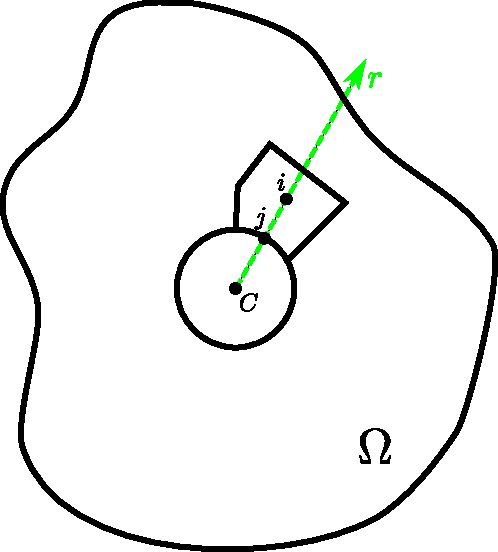
\includegraphics[width=0.4\linewidth]{radial_singularity.pdf}
\caption{Двусвязная область решения}
\label{fig:radial_singularity}
\end{figure}

Возьмём приграничную ячейку $i$ и граничную точку коллокации $j$.
Пусть точки $\vec C$, $\vec c_i$, $\vec c_j$ лежат на одной прямой. Координату
вдоль этой прямой будем называть $r$.
Будем считать, что граничное значение на внутреннем круге
сильно отличается (в большую или меньшую сторону) от
характерного значения $u$ в области расчёта.
Тогда в некотором приближении
решении в окрестности внутреннего круга можно
считать радиально симметричным: зависящим
только от $r$, но не от угла поворота радиус-вектора $\vec r$.
В приближении постоянного коэффициента диффузии такое решение будет удовлетворять уравнению 
\begin{equation*}
\frac 1r \dfr{}{r}\left( r \dfr{u}{r} \right) = 0.
\end{equation*}
Общим решением этого уравнение будет выражение
\begin{equation*}
u = A \ln r + B.
\end{equation*}
Коэффициенты $A$, $B$ выразим через значения
функции в точках коллокации:
\begin{equation*}
u(r_i) = u_i, \quad u(r_j) = u_j.
\end{equation*}
Тогда решение примет вид
\begin{equation*}
u(r) = \frac{\ln r - \ln r_i}{\ln r_j - \ln r_i}\left(u_j - u_i\right) + u_i.
\end{equation*}
Отсюда выразим нормальную производную на грани $\gamma_{ij}$:
\begin{equation} 
\label{eq:fvm_dudn_radial}
\left.\dfr{u}{n}\right|_{\gamma_{ij}} = -\left.\dfr{u}{r}\right|_{r=r_j} =  
\frac {1} {r_j} \, \frac{1}{\ln r_i - \ln r_j}\left(u_j - u_i\right).
\end{equation}
Это выражение будем использовать вместо
\cref{eq:fvm_dudn_dudc} для вычисления производной
на грани с логарифмической особенностью.

Учёт этой особенности можно реализовать за счёт модификации
коэффициента диффузии $\lambda_{ij}$ на граничной грани.
Выражение \cref{eq:fvm_dudn_radial}
можно свести к 
\cref{eq:fvm_dudn_lambda},
если считать диффузию в виде
\begin{equation}
\label{eq:fvm_ln_singularity_hij}
\lambda'_{ij} = \frac{\lambda_{ij}}{r_j} \frac{h_{ij}}{\ln r_i - \ln r_j}
\end{equation}

\subsubsection{Радиально-симметричная постановка}
\label{sec:fvm_radsym}
Теперь рассмотрим уравнение
\cref{eq:poissonnd_lam}
в цилиндрических координатах $(r, \theta, z)$ и радиально-симметричной постановке.
В частных производных определяющее уравнение запишется как
\begin{equation*}
\frac{1}{r}\dfr{}{r}\left( \lambda r \dfr{u}{r} \right) + \dfr{}{z}\left(\lambda \dfr{u}{z}\right) = f, \quad \dfr{u}{\theta} = 0.
\end{equation*}
Заметим, что общий вывод конечнообъёмной схемы
\cref{eq:fvm_lambda_ij_scheme}
использует только формулу Гаусса--Остроградского
\cref{eq:partint_div} в операторном виде.
Поэтому она будет справедлива в любой системе координат.

Особенность выбора радиально-симметричной постановки
проявится только в вычислении площади грани $|\gamma|$
и объёма ячейки $|E|$, которые в этой постановке являются телами
вращения вокруг оси $Oz$.
Вычислим объём как
\begin{equation*}
|E| = \int\limits_{E} d\vec x = \int\limits_0^{2\pi}\left(\iint\limits_{|E|_{rz}} r d r d z\right) d\phi  =
    2\pi \underbrace{\frac{1}{|E|_{rz}}\iint r \, d r d z}_{r_E} \, |E|_{rz} 
\end{equation*}
где $|E|_{rz}$ и $r_E$ -- объём и $r$--координата центра масс ячейки
в декартовой двумерной системе координат $(r, z)$.
Аналогичные рассуждения справедливы и для определения площади грани
через её двумерную площадь $|\gamma|_{rz}$ и центр масс $r_\gamma$.
Тогда окончательно запишем
\begin{equation}
\label{eq:fvm_radsym_measures}
\left|E\right| = 2 \pi r_E |E|_{rz}, \qquad
\left|\gamma\right| = 2 \pi r_\gamma |\gamma|_{rz}
\end{equation}


%\subsection{Метод конечных элементов}
\subsubsection{Формулировка}
Формулировка классического метода конечных элементов состоит из последовательного применения трёх методик:
\begin{itemize}
\item слабая (интегральная) постановка задачи с помощью метода взвешенных невязок,
\item использование метода Бубнова--Галёркина для записи интегральных соотношений для коэффициентов СЛАУ,
\item построение базисных функций с локальным носителем на основе конечноэлементной сетки.
\end{itemize}
\subsubsubsection{Метод взвешенных невязок}
TODO
\subsubsubsection{Метод Бубнова--Галёркина}
TODO
\paragraph{Пример с применением степенных базисных функций}
TODO
\subsubsubsection{Конечноэлементные базисные функции}
TODO
\subsubsection{Вывод СЛАУ для аппроксимации уравнения Пуассона}
\paragraph{Метод взвешенных невязок}
Исходное уравнение \cref{eq:poissonnd}
домножим на пробную функцию $q$ и проинтегрируем по
области решения
\begin{equation*}
-\arint{\nabla^2 u \, q}{\Omega}{\vec x} = \arint{f \, q}{\Omega}{\vec x}.
\end{equation*}
Чтобы сравнять порядок производной перед искомой функций $u$ и пробной
функцией $q$ применим формулу интегрирования по частям \cref{eq:partint_laplace_fg}:
\begin{equation*}
-\arint{\dfr{u}{n}\, q}{\partial\Omega}{s} + \arint{\nabla u \cdot \nabla q}{\Omega}{\vec x} = \arint{f \, q}{\Omega}{\vec x}.
\end{equation*}
Полученное выражение -- есть окончательная слабая постановка задачи.
\paragraph{Метод Бубнова--Галёркина}
В качестве пробной функции $q$ будем испльзовать набор базисных функций $\phi_i$, $i\in\overline{0, N-1}$.
По этому же базису разложим входящие в постановку скалярные функции $u$ и $f$.
Получим систему из $N$ линейных уравнений
\begin{equation*}
-\arint{\dfr{u}{n}\, \phi_i}{\partial\Omega}{s} +
\sum_{j=0}^{N-1}\left(\arint{\nabla \phi_j \cdot \nabla \phi_i}{\Omega}{\vec x}\right) u_j = \sum_{j=0}^{N-1}\left(\arint{\phi_j \, \phi_i}{\Omega}{\vec x}\right) f_j.
\end{equation*}
Первый из интегралов будет не равным нулю только для строк $i$, соответсвтующих
граничным узлам (базисам). Во всех остальных базисная функция 
согласно свойству согласованности будет равна нулю.
Тогда строки СЛАУ, соответсвующие внутренним узлам, примут вид
\begin{equation*}
\mat{S} u = \mat{b},
\quad \mat {b} = \mat M f,
\end{equation*}
где элементы матрицы масс $\mat M$ и матрицы жёсткости $\mat S$ будут равны
\begin{align}
\label{eq:fem_mass_mat}
&M_{ij} = \arint{\phi_j \phi_i}{\Omega}{\vec x},\\
\label{eq:fem_stiff_mat}
&S_{ij} = \arint{\nabla \phi_j \cdot \nabla \phi_i}{\Omega}{\vec x}.
\end{align}

Отдельно рассмотрим вычисление интеграла от некоторой функции $g$ в 
рамках аппроксимации Бубнова--Галёркина:
\begin{equation*}
\arint{g}{\Omega}{\vec x} = \sum_{j=0}^{N-1}V_i g_i,
\end{equation*}
где элементы ветора нагрузок $\mat V$ будут равны
\begin{equation}
\label{eq:fem_load_vec}
V_{i} = \arint{\phi_i}{\Omega}{\vec x}.
\end{equation}

\subsubsubsection{Одномерный пример}
TODO
\subsubsection{Техника сборки конечноэлементных векторов и матриц}
\subsubsubsection{Элементные вектора}
Распишем интеграл \cref{eq:fem_load_vec} по области $\Omega$
как сумму интегралов по отдельным элементам $E_m$.
При вследствии свойства локальности конечноэелементных базисов
в сумме можно оставить лишь элементы, инцидентные базису $i$:
\begin{equation*}
V_{i} = \arint{\phi_i}{\Omega}{\vec x} = \sum_{m \in \rm J^i} \arint{\phi^{(m)}_i}{E_m}{\vec x}.
\end{equation*}
Определим элементный вектор нагрузок $V^{(m)}$ 
как 
\begin{equation}
\label{eq:fem_elem_load_vector}
V^{(m)}_j = \arint{\phi^{(m)}_{g(j)}}{E_m}{\vec x}.
\end{equation}
Его размерность равна количеству степеней свободы элемента $N^{(m)}$.
Здесь запись $g(j)$ -- это перевод локального внутриэлементного индекса $j\in\overline{0, N^{(m)}-1}$
в глобальный индекс $i\in\overline{0, N}$.
\subsubsubsection{Элементные матрицы}
Аналогично можно расписать интегралы из \cref{eq:fem_mass_mat,eq:fem_stiff_mat}
через элементные интегралы. В частности для матрицы масс получим
\begin{equation*}
M_{ij} = \arint{\phi_i \phi_j}{\Omega}{\vec x} = \sum_{m \in \rm J^i} \arint{\phi^{(m)}_i \, \phi^{(m)}_j}{E_m}{\vec x}.
\end{equation*}
а выражение для локальной матрицы масс размерности $N^{(m)}\times N^{(m)}$ примет вид
\begin{equation}
\label{eq:fem_elem_mass_matrix}
M^{(m)}_{kl} = \arint{\phi^{(m)}_{g(k)} \, \phi^{(m)}_{g(l)}}{E_m}{\vec x}.
\end{equation}
По аналогии элементная матрица жёсткости запишется как
\begin{equation}
\label{eq:fem_elem_stiff_matrix}
S^{(m)}_{kl} = \arint{\nabla \phi^{(m)}_{g(k)} \cdot \nabla \phi^{(m)}_{g(l)}}{E_m}{\vec x}.
\end{equation}

\subsubsubsection{Алгоритм сборки}
После того, как элементные вектора/матрицы для
искомого интеграла определены, следует применить алгоритм
элементной сборки. Для этого понадобится
таблица связность \quo{элемент-индексы базисов}.
В простейшем случае линейных лагранжевых базисов
эта таблица эквивалентна геометрической таблице \quo{ячейка-узлы}.
Назовём эту таблицу $glob$. Тогда псеводкод для сборки вектора примет вид
\begin{equation}
\label{eq:fem_vector_assemble}
\begin{array}{ll}
V_i = 0                                                      & \textrm{-- инициализируем глобальный вектор нулями}\\
\textbf{for } m = \overline{0, N-1}                          & \textrm{-- цикл по конечным элементам}\\
\qquad N^m = dof(m)                                                   & \textrm{-- количество степеней свободы у элемента}\\ 
\qquad \textbf{for } i = \overline{0, N^m-1}              & \textrm{-- цикл по базисам внутри элемента}\\
\qquad \qquad g = glob(m, i)                                & \textrm{-- глобальный индекс локального базиса}\\
\qquad \qquad V_{g} \pluseq  V^{m}_i                              & \\
\qquad \textbf{endfor}                                       & \\
\textbf{endfor}
\end{array}
\end{equation}
В аналогичном алгоритме для матрицы добавится ещё один цикл:
\begin{equation}
\label{eq:fem_matrix_assemble}
\begin{array}{ll}
M_{ij} = 0                                                      & \textrm{-- инициализируем глобальную матрицу нулями}\\
\textbf{for } m = \overline{0, N-1}                          & \textrm{-- цикл по конечным элементам}\\
\qquad N^m = dof(m)                                                   & \textrm{-- количество степеней свободы у элемента}\\ 
\qquad \textbf{for } i = \overline{0, N^m-1}              & \textrm{-- цикл по базисам внутри элемента}\\
\qquad \qquad \textbf{for } j = \overline{0, N^m-1}              & \textrm{-- цикл по базисам внутри элемента}\\
\qquad \qquad \qquad g = glob(m, i)                                & \textrm{-- глобальный индекс локального базиса}\\
\qquad \qquad \qquad h = glob(m, j)                               & \\
\qquad \qquad \qquad M_{gh} \pluseq  M^{m}_{ij}                              & \\
\qquad \qquad \textbf{endfor}                                       & \\
\qquad \textbf{endfor}                                       & \\
\textbf{endfor}
\end{array}
\end{equation}
\subsubsection{Вычисление элементных интегралов в модельном пространстве}
Будем вычислять элементные интегралы \cref{eq:fem_elem_mass_matrix,eq:fem_elem_stiff_matrix,eq:fem_elem_load_vector}
в модельном пространстве $\vec \xi$.
Для этого введём преобразование координат $\vec x \rightarrow \vec \xi$ согласно п.\ref{sec:coo_transform}.
Интеграл для определения локальной матрицы масс \cref{eq:fem_elem_mass_matrix} 
в модельных координатах распишется согласно формуле \cref{eq:dxideta_integral}
\begin{equation}
\label{eq:fem_mass_matrix_xi}
M^{(m)}_{ij} = \arint{\N^{(m)}_i \N^{(m)}_j|J^{(m)}|}{\tilde E_m}{\vec \xi}
\end{equation}
Здесь $\tilde E_m$ -- параметрический образ конечного элемента $E^k$,
$|J^{(m)}(\vec \xi)|$ - Якобиан преобразования для $m$-ого элемента,
$\N^{(m)}_i(\vec \xi)$ -- функция формы, или часть базисной фукнции, заданная в $m$-ом элементе в модельных координатах.
То есть
\begin{equation*}
\N_i^{(m)}(\vec \xi) = \phi_{g(i)}^{(m)}(\vec x(\vec \xi)).
\end{equation*}
Локальный вектор нагрузок записывается из соотношения \cref{eq:fem_elem_load_vector}:
\begin{equation}
\label{eq:fem_load_vector_xi}
V^{(m)}_{i} = \arint{\N^{(m)}_i |J^{(m)}|}{\tilde E_m}{\vec \xi}
\end{equation}
Локальная матрица жёсткости из \cref{eq:fem_elem_stiff_matrix}:
\begin{equation}
\label{eq:fem_stiff_matrix_xi}
S^{(m)}_{ij} = \arint{\nabla_{\vec x} \N^{(m)}_i \cdot \nabla_{\vec x} \N^{(m)}_j |J^{(m)}|}{\tilde E_m}{\vec \xi}
\end{equation}
Здесь $\nabla_{\vec x} \N^{m}_i$ -- градиент shape-функции (заданного в модельном пространстве) по физическим координатам.
Для его вычисления следует воспользоваться формулами \cref{eq:vec_grad_dx}

%\subsubsubsection{Треугольный элемент. Линейный двумерный базис}
%Матрица масс (из \cref{eq:mass_matrix}):
%\begin{equation}
%\label{eq:mass_matrix_lintri}
%M^E_{ij} = \int\limits_0^1 \int\limits_0^{1-\xi} \phi_i(\xi, \eta) \phi_j(\xi, \eta) |J| \, d\eta d\xi =
%\frac{|J|}{24}\left(
%\begin{array}{ccc}
%2 & 1 & 1 \\
%1 & 2 & 1 \\
%1 & 1 & 2
%\end{array}
%\right)
%\end{equation}


%\section{Нестационарное уравнение переноса}

\subsection{Двухслойные схемы для нестационарных уравнений}

\subsubsection{Определение}

Рассмотрим дифференциальное уравнение вида

\begin{equation}
    \label{eq:nonstat_common}
    \dfr{u}{t} = f, \quad f(x, t) = Lu(x, t) + g(x, t)
\end{equation}
где $L$ -- произвольный пространственный дифференциальный оператор.
При использовании двухслойной схемы аппроксимации производная по времени записывается в
виде конечной разности с шагом $\dt$, которая может приближать производную
в одном из трёх моментов времени:

\begin{equation}
    \label{eq:nonstat_dt_appr}
    \begin{array}{llll}
        \dfrac{u(t+\dt) - u(t)}{\dt} = 
            & \quad \left.\ddfr{u}{t}\right|_{t}
            & + o(\dt)
            & -\text{ разность вперёд};\\[5pt]
        \phantom{a}
            & \quad \left.\ddfr{u}{t}\right|_{t+\dt}
            & + o(\dt)
            & -\text{ разность назад};\\[5pt]
        \phantom{a}
            & \quad \left.\ddfr{u}{t}\right|_{t+\frac{\dt}{2}}
            & + o(\dt^2)
            & -\text{ симметричная разность.}
    \end{array}
\end{equation}

Момент времени $t$ будем называть текущим временн\'{ы}м слоем,
момент $t + \dt$ -- следующим,
а момент $t+\dt/2$ -- промежуточным.
Считается, что
значение функции на текущий момент времени $u(t)$ известно, а
значение на следующий момент $u(t+\dt)$ подлежит определению.

\subsubsubsection{Явная схема}

При использовании разности назад уравнение \eqref{eq:nonstat_common}
в полудискретизованном (то есть дискретизованном только по времени, но не по пространству) виде
запишется как
\begin{equation*}
    \frac{u(x, t+\dt) - u(x)}{\dt} - L u(x, t) = g(x, t)
\end{equation*}
или, после переноса всех известных слагаемых вправо
\begin{equation}
    \label{eq:nonstat_explicit}
    u(x, t+\dt) = \left(E + \dt L\right) u(x, t) + \dt g(x, t).
\end{equation}
Здесь $E$ -- единичный оператор.
Схема \eqref{eq:nonstat_explicit} называется явной схемой
и имеет первый порядок точности.

\subsubsubsection{Неявная схема}

Выбрав разность назад из выражения \eqref{eq:nonstat_dt_appr}
полудискретизованная схема для уравнения \eqref{eq:nonstat_common} примет вид
\begin{equation*}
    \frac{u(x, t+\dt) - u(x)}{\dt} - L u(x, t+\dt) = g(x, t+\dt).
\end{equation*}
В результате преобразования получим неявную схему первого порядка точности
\begin{equation}
    \label{eq:nonstat_implicit}
    \left(E-\dt L\right) u(x, t+\dt) = u(x, t) + \dt g(x, t + \dt).
\end{equation}

\subsubsubsection{Схема Кранка--Николсон}

Подставим симметричную разность из \eqref{eq:nonstat_dt_appr}
в уравнение \eqref{eq:nonstat_common}. Формально получим
\begin{equation*}
    \frac{u(x, t+\dt) - u(x)}{\dt} - L u(x, t+\frac{\dt}{2}) = g(x, t+\frac{\dt}{2}).
\end{equation*}

Для определения выражения функций на промежуточном временном слое
распишем значение $u$ на текущем и следующем слоях в ряд Тейлора
относительно значения на момент $t+\dt/2$:
\begin{align*}
    u\left(t\right)      &= u\left(t+\frac{\dt}{2}\right) - \left.\frac{\dt}{2}\dfr{u}{t}\right|_{t+\frac{\dt}{2}} + o(\dt^2)\\
    u\left(t+\dt\right) &= u\left(t+\frac{\dt}{2}\right) + \left.\frac{\dt}{2}\dfr{u}{t}\right|_{t+\frac{\dt}{2}} + o(\dt^2)
\end{align*}
Взяв полусумму этих выражений получим аппроксимацию функции на промежуточном слое:
\begin{equation}
    \label{eq:nonstat_cn_appr}
    u\left(x, t + \frac{\dt}{2}\right) = \frac12u\left(x, t\right) + \frac12u\left(x, t+\dt\right) + o(\dt^2)
\end{equation}
Аналогичная запись справедлива и для свободного члена $g$.
Если оператор $L$ -- нестационарный или нелининый, то аппроксимацию \eqref{eq:nonstat_cn_appr}
следует записывать для всего выражения $Lu$:
\begin{equation*}
    \left(Lu\right)_{t+\frac{\dt}{2}} = \frac12\left(Lu\right)_{t} + \frac12\left(Lu\right)_{t+\dt} + o(\dt^2)
\end{equation*}


С учётом \eqref{eq:nonstat_cn_appr} симметричная разностная схема
запишется как
\begin{equation*}
    \frac{u(x, t+\dt) - u(x)}{\dt} - \frac12L u(x, t) - \frac12 L u(x, t + \dt) = \frac12 g(x, t) + \frac12 g(x, t+\dt)
\end{equation*}
или
\begin{equation}
    \label{eq:nonstat_cn}
    \left(E-\frac{\dt}{2} L\right) u(x, t+\dt) = \left(E + \frac{\dt}{2} L\right) u(x, t) + \frac{\dt}{2} \left(g(x, t) + g(x, t + \dt)\right).
\end{equation}
Такая схема называется схемой Кранка--Николсон и имеет второй порядок аппроксимации по времени.

В случае, если оператор $L$ зависит от времени, то
в левой части схемы \eqref{eq:nonstat_cn} его нужно
брать на следующем временном слое, а в правой -- на текущем.

\subsubsubsection{Обобщённая двухслойная схема}

Выражения
\eqref{eq:nonstat_explicit},
\eqref{eq:nonstat_implicit},
\eqref{eq:nonstat_cn}
можно записать в обобщённой форме
\begin{equation}
    \label{eq:nonstat_theta}
    \left(E-\theta\dt L\right) u(x, t+\dt) = \left(E + \left(1 - \theta\right)\dt L\right) u(x, t) + \left(1 - \theta\right) g(x, t) + \theta g(x, t + \dt).
\end{equation}
Коэффициент $\theta$ -- степень неявности схемы:
\begin{itemize}
\item $\theta = 0$ -- явная схема \eqref{eq:nonstat_explicit},
\item $\theta = 1$ -- полностью неявная схема \eqref{eq:nonstat_implicit},
\item $\theta = 1/2$ -- схема Кранка--Николсон \eqref{eq:nonstat_cn}.
\end{itemize}

Отметим, что только при $\theta = 1/2$ схема \eqref{eq:nonstat_theta} имеет второй порядок точности по времени.
Для других значений (в том числе промежуточных) схема будет иметь ошибку первого порядка $o(\dt)$.

\subsection{Схемы высокого порядка точности}
Существуют два подхода к построению схем дискретизации по времени произвольного высокого порядка:
первый из них предполагает использование нескольких временных слоев: $t+\dt, t, t-\dt, t-2\dt, ...$, второй -- использование
большого количества промежуточных точек на единственном временном отрезке: $t+c_i\dt, c_i\in[0, 1]$.
Первый подход используется для построения схем Адамса, второй -- схем Рунге--Кутта.

\subsubsection{Многослойные схемы. Схемы Адамса}
В общем виде многослойную расчётную схему можно записать в виде
\begin{equation}
\label{eq:nonstat_multilayer}
\sum\limits_{i=1}^{s} a_i u_i = \dt \sum\limits_{i=1}^{s} b_i f_i.
\end{equation}
Здесь нижние индексы функций использованы для указания временного слоя:
\begin{equation*}
\begin{aligned}
&u_i = u(x, t + (i+1-s)\dt),\\
&f_i = g(x, t + (i+1-s)\dt) - Lu_i,
\end{aligned}
\end{equation*}
а $s$ -- это общее количество используемых временных слоёв.
Значение всех функций на слоях $i<s$ считаются известными, а значение $u_s$ на последнем (текущем) слое подлежит определению.
Коэффициенты $a_i$. $b_i$ определяют конкретную схему.
Для однозначности принято задавать коэфиициет перед значением $u$ на текущем слое равным единице: $a_s = 1$.
Так, для двухслойной ($s=2$) схемы Кранка--Николсон \cref{eq:nonstat_cn} эти коэффициенты примут вид:
\begin{align*}
&a_1 = -1, \quad a_2 = 1,\\
&b_1 = 1/2, \quad b_2 = 1/2.
\end{align*}
Для того чтобы схема, записанная в общем виде \cref{eq:nonstat_multilayer}, была явной,
необходимо, чтобы выполнялось условие $b_s = 0$.

\subsubsubsection{Явные схемы Адамса--Башфорта}
Запишем интерполяционный полином для правой части уравнения \cref{eq:nonstat_common}
по значениям на предыдущих временных слоях $f_i, i<s$:
\begin{equation*}
p(t) = \sum\limits_{i=1}^{s-1}\left(f_i \prod\limits_{\substack{m=1\\m \neq i}}^{s-1} \frac{t - t_i}{t_m - t_i} \right).
\end{equation*}
Порядок аппроксимации этого полинома на единицу больше его степени. С учётом 
$t_{i+1} - t_{i} = \dt$ можно записать
\begin{equation*}
f(t) = p(t) + o(\dt^{s-1}).
\end{equation*}

Далее проинтегрируем уравнение по текущему временному отрезку: $[t_{s-1}, t_{s}]$:
\begin{equation*}
u_s - u_{s-1} = \sum_{i=1}^{s-1}\left( f_i \int\limits_{t_{s-1}}^{t_s} \prod \limits_{\substack{m=0\\m\neq i}}^{s-1} \frac{t - t_i}{t_m - t_i}\, dt \right).
\end{equation*}

Отсюда коэффициенты в общей форме \cref{eq:nonstat_multilayer} примут вид
\begin{equation*}
a_i = 
\begin{cases}
1,  &\quad i = s\\
-1, &\quad i = s-1\\
0,  &\quad i < s-1
\end{cases}
\qquad
b_i =
\begin{cases}
0, &\quad i = s\\[10pt]
\displaystyle\frac{1}{\dt}\int\limits_{t_{s-1}}^{t_s} \prod \limits_{\substack{m=0\\m\neq i}}^{s-1} \frac{t - t_i}{t_m - t_i}\, dt, &\quad i < s.
\end{cases}
\end{equation*}

Примеры трёх-, четырех- и пятислойной явных схем приведены ниже:
\begin{align*}
&\frac{u_3 - u_2}{\dt} = \frac{3f_2 - f_1}{2} + o(\dt^2),\\
&\frac{u_4 - u_3}{\dt} = \frac{23 f_3 - 16 f_2 + 5 f_1}{12} + o(\dt^3),\\
&\frac{u_5 - u_4}{\dt} = \frac{55 f_4 - 59 f_3 + 37 f_2 - 9 f_1}{24} + o(\dt^4).
\end{align*}

\subsubsubsection{Неявные схемы Адамса--Мультона}
Теперь снимем требование явности и запишем интерполяционный полином для правой части исходного уравнения \cref{eq:nonstat_common} с использованием $s$ точек:
\begin{equation*}
p(t) = \sum\limits_{i=1}^{s}\left(f_i \prod\limits_{\substack{m=1\\m \neq i}}^{s} \frac{t - t_i}{t_m - t_i} \right).
\end{equation*}
Тогда порядок аппроксимации этого полинома будем на единицу больше, чем для полинома явного метода.
Далее, проинтегрируем исходное уравенение по отрезку $t_{s-1}, t_s$ и получим коэффициенты общей формы \cref{eq:nonstat_multilayer}:
\begin{equation*}
a_i = 
\begin{cases}
1,  &\quad i = s\\
-1, &\quad i = s-1\\
0,  &\quad i < s-1
\end{cases}
\qquad
b_i =
\displaystyle\frac{1}{\dt}\int\limits_{t_{s-1}}^{t_s} \prod \limits_{\substack{m=0\\m\neq i}}^{s} \frac{t - t_i}{t_m - t_i}\, dt.
\end{equation*}

Двуслойная схема Адама--Мультона будет аналогична неявной двухслойной схеме \cref{eq:nonstat_implicit},
трёхслойная -- схеме Кранка--Николсон \cref{eq:nonstat_cn}. Примеры схемы высоких порядков представлены ниже:
\begin{align*}
&\frac{u_3 - u_2}{\dt} = \frac{5f_3 +  8 f_2 - f_1}{12} + o(\dt^3),\\
&\frac{u_4 - u_3}{\dt} = \frac{9 f_4 + 19 f_3 - 5 f_2 + f_1}{24} + o(\dt^4),\\
&\frac{u_5 - u_4}{\dt} = \frac{251 f_5 + 646 f_4 - 264 f_3 + 106 f_2 - 19 f_1}{720} + o(\dt^5).
\end{align*}

\subsubsection{Схемы Рунге-Кутта}
TODO

\subsection{Устойчивость расчётных схем}
\label{sec:stability_analysis}

\subsubsection{Дискретизация по времени как итерационный процесс}

\subsubsubsection{Двухслойный итерационный процесс}

Простой двухслойный итерационный процесс определяется как
\begin{equation}
    \label{eq:nonstat_common_iter}
    u^{n+1} = A u^{n} + b,
\end{equation}
где $n$ -- индекс итерационного слоя,
$A$ -- оператор преобразования,
$b$ -- свободный член.

Определение значения функции на следующий момент времени $u(t+\dt)$ 
по двухслойной схеме \eqref{eq:nonstat_theta} можно представить как простой итерационный процесс \eqref{eq:nonstat_common_iter}, где
\begin{align*}
    A &= \left(E - \theta \dt L \right)^{-1} \left(E + (1 - \theta) \dt L \right), \\\\
    b &= \left(E - \theta \dt L \right)^{-1} \left( \theta g\left(x, t + \dt\right) + \left(1 - \theta\right) g\left(x, t\right) \right).
\end{align*}

Итерационный процесс называется сходящимся, если
\begin{equation*}
    \lim_{n=\infty} \left\lVert u^{n+1} - u^{n} \right\rVert = 0.
\end{equation*}

\subsubsubsection{Устойчивость итерационного процесса}
\label{sec:ScalarIter}

Рассмотрим два простых итерационных процесса,
имеющих на нулевом слое значение $u^0 = 1$:
\begin{align*}
    {\rm (I)}:\quad  &u^{n+1} = 2 u^{n} - 1, \\
    {\rm (II)} :\quad  &u^{n+1} = 0.5 u^{n} + 0.5.
\end{align*}
Оба этих процесса при выбранном начальном приближении, очевидно, сходятся.
На каждой итерации справделиво $u^n = 1$.
Возмутим начальное условие: пусть
\begin{equation*}
    u^0 = 1 + \eps,
\end{equation*}
и проведём итерации.
\begin{equation*}
    \def\arraystretch{1.7}
    \begin{array}{c|c|c}
        & {\rm (I)}  &  {\rm (II)} \\
        \hline
        u^1 & 1 + 2\eps & 1 + \dfrac{\eps}{2} \\
        \hline
        u^2 & 1 + 4\eps & 1 + \dfrac{\eps}{4} \\
        \hline
        u^3 & 1 + 8\eps & 1 + \dfrac{\eps}{8} \\
        \hline
        ... & & \\
        \hline
        u^\infty & \infty & 1 \\
    \end{array}
\end{equation*}

Видно, что в процессе $\rm (I)$ \cvar{u} стремится к бесконечности,
в то время, как в процесс $\rm (II)$ \cvar{u} сохраняет своё начальное значение.

Свойство итерационных процессов уменьшать малые возмущения называется устойчивостью.
В примере выше процесс $\rm (I)$ является неустойчивым, а процесс $\rm (II)$ -- устойчивым.

Нетрудно видеть, что для рассматриваемого скалярного итерационного процесса,
условие устойчивости запишется в виде $|A| \leq 1$.

\subsubsubsection{Источники возмущений}

На практике возникновение возмущений в решениях неизбежно:
они могут быть следствием ошибок дискретизации функций и операторов,
погрешностей решения СЛАУ, ошибок при проведении арифметических
операций на числах с плавающей точкой и т.д.
Поэтому любой итерационный процесс, используемый для решений
математических задач, должен быть устойчив.

Возникновение непреднамеренных ошибок вследствии компьютерного округления можно проиллюстрировать на примере
программы, в которой рассматривается сходящийся для любого начального условия, но неустойчивый итерационный процесс
\begin{equation*}
    u^{n+1} = 10 u^{n} - 9 u^{0}.
\end{equation*}

\begin{minted}[linenos=false]{c++}
const double u0 = 0.625;
double u = u0;
for (int i=0; i<1000; ++i){
    u = 10*u - 9*u0;
}
std::cout << u << std::endl;
\end{minted}

Если начальное значение может быть точно представлено в
числах с плавающей точкой (путём конечной суммы степеней двойки),
то арифметическая ошибка не возникает.
Так, представленный выше код на выходе печатает ожидаемое $u=0.625$.
Потому что начальное приближение может быть разложено как $u^0 = 2^{-1} + 2^{-3}$.

Однако, если заменить начальное приближение на любое число,
которое не может быть записано точно во floating-point формате,
то процесс быстро уходит в бесконечность.
Например, для $u^0 = 0.626$ бесконечные (непредставимые в машинном формате) значения
появляются на 324-ой итерации,
а при переключении на работу в числах одинарной точности `float` -- уже на 46-ой.

\subsection{Свойства двухслойной расчётной схемы}
TODO

\subsection{Аппроксимация уравнения переноса с ограничением потока}

\subsubsection{Схемы первого и второго порядка точности}
Рассмотрим уравнение переноса в одномерной постановке

\begin{equation*}
\label{eq:tvd_transport}
\dfr{u}{t} + U\dfr{u}{x} = 0
\end{equation*}
Все дальнейшие выкладки будем приводить исходя из условия положительности скорости переноса $U > 0$.

Рассмотрим два вида пространственной аппроксимации конвективного слагаемого на равномерной сетке: схемой против потока и симметричной схемой
\begin{align}
& \dfr{u_i}{t} + U \frac{u_i - u_{i-1}}{h} = 0, \label{eq:tvd_upwind}\\
& \dfr{u_i}{t} + U \frac{u_{i+1} - u_{i-1}}{2h} = 0. \label{eq:tvd_sym}
\end{align}
Первая схема является (условно) устойчивой но при этом обладает первым
порядком аппроксимации. Вторая неустойчива, но имеет порядок $o(h^2)$.
Идея методов аппроксимации с ограничением потока состоит в том,
чтобы на основе комбинации первой и второй схем
построить устойчивое решение, имеющее ``почти везде'' второй порядок аппроксимации.

Запишем эти аппроксимации в общем виде:
\begin{equation}
\label{eq:tvd_appr_with_f}
\dfr{u_i}{t} = \frac{f_{i-\sfrac12} - f_{i+\sfrac12}}{h}.
\end{equation}
Здесь $f_{i+\sfrac12}$ -- численный поток, который в зависимости от выбранной схемы будет равен
\begin{equation}
\label{eq:tvd_fhl}
\begin{aligned}
&f^L_{i+\sfrac12} = U u_i                            &\text{-- схема против потока}\\
&f^H_{i+\sfrac12} = U \frac{u_i + u_{i+1}}{2}        &\text{-- симметричная схема}.
\end{aligned}
\end{equation}
Здесь $f^L$, $f^H$ означают потоки низкого (Low) и высокого (High) порядка аппроксимации.

Аппроксимацию с ограничением потока запишем в виде
\begin{equation}
\label{eq:tvd_f}
f_{i+\sfrac12} = f^L_{i+\sfrac12} + \Phi_{i+\sfrac12} \left( f^H_{i+\sfrac12} - f^L_{i+\sfrac12} \right).
\end{equation}
$\Phi$ в этой записи называется ограничителем, который служит
переключателем: при $\Phi = 0$ мы получаем схему первого порядка, при $\Phi=1$ -- схему второго порядка.

Далее будем выбирать $\Phi$ таким образом, чтобы не допустить возникновения осцилляций в численном решении.

\subsubsection{Условие TVD}
В качестве критерия, характеризующего возникновение и развитие осцилляций, выберем полную вариацию:
\begin{equation}
\label{eq:tvd_tv}
\begin{WithArrows}
TV(u) =& \displaystyle\int\left| \nabla u \right|\,dx =           \Arrow{в одномерном случае}\\[10pt]
      =& \displaystyle\int\left| \dfr{u}{x} \right| \, dx =       \Arrow{для сеточной функции}\\[10pt]
      =& \displaystyle\sum_{i}\left| u_i - u_{i-1}\right|.
\end{WithArrows}
\end{equation}
Условие уменьшения осцилляций в решении на следующем временном слое примет вид
\begin{equation*}
TV(\hat u) \leq TV(u).
\end{equation*}
Численные схемы, удовлетворяющие этому условию, называются TVD (Total variation diminishing) схемами.

Запишем численную схему в общем виде
\begin{equation}
\label{eq:tvd_harten}
\dfr{u_i}{t} = c_{i-\sfrac12} (u_{i-1} - u_{i}) + c_{i+\sfrac12} (u_{i+1} - u_{i}).
\end{equation}
Согласно теореме Хартена такая схема удовлетворяет свойству TVD, если $c_{i\pm\sfrac12} \geq 0$.
Схема против потока \cref{eq:tvd_upwind} является TVD-схемой:
$$c_{i-\sfrac12} = \frac{U}{h}, \quad c_{i+\sfrac12} = 0,$$
а симметричная схема \cref{eq:tvd_sym} -- нет:
$$c_{i-\sfrac12} = \frac{U}{2h}, \quad c_{i+\sfrac12} = -\frac{U}{2h}.$$

Подставляя уравнение \cref{eq:tvd_f} в \cref{eq:tvd_appr_with_f} 
и приводя к форме \cref{eq:tvd_harten} получим
\begin{equation}
\label{eq:tvd_phi_condition1}
\dfr{u_i}{t} = \frac{U}{2h}\left( 2 - \Phi_{i-\sfrac12} \right) \left( u_{i-1} - u_{i} \right)
               +\frac{U}{2h}\left(-\Phi_{i+\sfrac12} \right) \left( u_{i+1} - u_i\right)
\end{equation}
То есть для удовлетворения свойства TVD необходимо, чтобы $\Phi \leq 0$.
Для второго порядка точности требуется $\Phi = 1$. То есть линейные схемы TVD не могут иметь высокий порядок точности.

\subsubsection{Нелинейные TVD схемы}
Для того, чтобы преодолеть это ограничение, будем строить нелинейные схемы.
Общая идея построения таких схем состоит в том, чтобы выбрать такую $\Phi$,
при которой второе слагаемое равенства \cref{eq:tvd_phi_condition1} можно
было отнести к первому. То есть можно бы было записать
\begin{equation}
\label{eq:tvd_phi_condition2}
\Phi_{i+\sfrac12}(u_{i+1} - u_{i}) = -\Phi'_{i+\sfrac12} (u_{i-1} - u_{i}).
\end{equation}
Тогда условием TVD станет выражение
\begin{equation}
\label{eq:tvd_phi_condition3}
2 - \Phi_{i-\sfrac12} + \Phi'_{i+\sfrac12} \geq 0.
\end{equation}

Для характеристики поведения функции выберем соотношение наклонов (slope ratio),
который в одномерном виде запишется в виде:
\begin{equation}
\label{eq:tvd_ri}
r_i = \frac{u_i - u_{i-1}}{u_{i+1} - u_{i}}
\end{equation}
Нелинейность схемы будет выражаться в зависимости
\begin{equation*}
\Phi_{i+\sfrac12} = \Phi(r_i).
\end{equation*}

Из \cref{eq:tvd_phi_condition2} следует
\begin{equation*}
\Phi'_{i+\sfrac12} = \frac{\Phi(r_i)}{r_i}
\end{equation*}
а неравенство $\label{eq:tvd_phi_condition4}$
перепишется в виде
\begin{equation*}
\label{eq:tvd_phi_condition5}
2 - \Phi(r_i) + \frac{\Phi(r_i)}{r_i} \geq 0.
\end{equation*}
Чтобы из этого условия получить ограничение для $\Phi$, явно не зависящее от $r_i$, потребуем
\begin{equation}
\label{eq:tvd_phi_condition4}
\Phi\left(\frac{1}{r_i}\right) = \frac{\Phi(r_i)}{r_i}.
\end{equation}
Тогда неравентсво \cref{eq:tvd_phi_condition3} примет вид
\begin{equation*}
\label{eq:tvd_phi_condition6}
2 - \Phi(r_i) + \Phi\left(\frac{1}{r_i}\right) \geq 0.
\end{equation*}
Отсюда получим условие для $\Phi$:
\begin{equation}
\label{eq:tvd_phi_condition7}
0 \leq \Phi(r_i) \leq 2.
\end{equation}

Дополнительно потребуем, чтобы в точках с гладким поведением функции использовать схему второго порядка точности:
\begin{equation}
\label{eq:tvd_phi_condition8}
\Phi(1) = 1
\end{equation}
а в точках локального экстремума (которые особенно подвержены появлению осцилляций) гарантировать переключение на схему первого порядка:
\begin{equation}
\label{eq:tvd_phi_condition9}
\Phi(r\leq0) = 0.
\end{equation}

Таким образом, для построения TVD схемы, функция ограничитель должна удовлетворять условиям
\cref{eq:tvd_phi_condition4,eq:tvd_phi_condition7,eq:tvd_phi_condition8,eq:tvd_phi_condition9}.
Ниже представлены некоторые часто используемые ограничители, удовлетворяющие этим свойствам:
\begin{equation}
\label{eq:tvd_limiter}
\Phi(r) = \left\{
\begin{array}{ll}
\max(0, \min(r, 1))                   & \text{-- minmod};\\[10pt]
\dfrac{r + |r|}{1+|r|}                & \text{-- Van Leer}; \\[10pt]
\max(0, \min(2r, \dfrac{1+r}{2}, 2)   & \text{-- monotonized central (MC)}; \\[10pt]
\max(0, \min(2, r), \min(1, 2 r))     & \text{-- superbee}.
\end{array}
\right.
\end{equation}

\subsection{TVD-схемы для неструктурированных конечнообъёмных сеток}
\label{sec:tvd_fvm}
Рассмотрим многомерное уравнение переноса
\begin{equation}
\nonumber
\dfr{u}{t} + \vec U \cdot \nabla u = 0.
\end{equation}

Применим конечнообъёмную процедуру
для получения слабой интегральной постановки задачи.
Для этого проинтегрируем это уравнение
по конечному объёму $E_i$ 
и применим формулу интегрирования по частям.
Получим
\begin{equation}
\label{eq:tvd_fvm_transport}
\left| V_i \right|
\dfr{u}{t}
+ \sum_{j\in {\rm nei}(i)} {f_{ij} \left|\gamma_{ij}\right|}
= 0, \quad f_{ij} = u_{ij} U_{ij}.
\end{equation}
Здесь $|V_i|$ -- объём конечного элемента,
${\rm nei}(i)$ -- совокупность
всех точек коллокации, инцидентных ячейке $i$
(центров соседних ячеек и соседних граничных граней),
$f_{ij}$ -- поток из точки коллокации $i$ в точку коллокации $j$,
$|\gamma_{ij}|$ --
площадь грани
конечного объёма $i$, через
которую этот объём соединяется с точкой коллокации $j$,
$u_{ij}$ -- значение функции $u$, отнесённое к этой грани,
$U_{ij}$ -- скорость потока в направлении внешней по отношению
к ячейке $i$ нормали.

Для потока справедливо
\begin{equation}
\label{eq:tvd_fij_fji}
f_{ij} = -f_{ji}.
\end{equation}
То есть для вычисления потока на грани достаточно найти значение для одного направления.
Выберем это направление $\overrightarrow{ij}$ таким образом, чтобы $U_{ij} > 0$ (рис.~\ref{fig:fvm_tvd}).


\begin{figure}[h!]
\centering
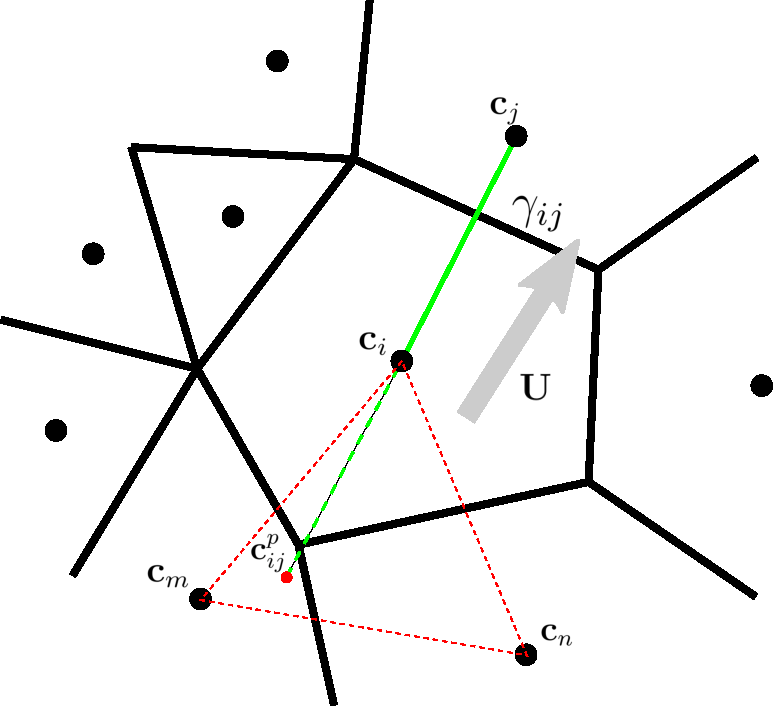
\includegraphics[width=0.4\linewidth]{fvm_tvd.pdf}
\caption{Вспомогательный узел $\vec c^p_{ij}$ на конечнообъёмной сетке}
\label{fig:fvm_tvd}
\end{figure}

Будем считать, что скорость переноса $U$ -- известная функция.
Тогда запишем значения потоков высокого и низкого порядка согласно \cref{eq:tvd_fhl}:
\begin{equation}
\label{eq:tvd_fhl_fvm}
\begin{aligned}
&f^L_{ij} = U_{ij} u_i                 &\text{-- схема против потока}\\
&f^H_{ij} = U_{ij} \frac{u_i + u_j}{2} &\text{-- симметричная схема}.
\end{aligned}
\end{equation}

Поток при этом запишется по аналогии с \cref{eq:tvd_f}:
\begin{equation}
\label{eq:tvd_f_fvm}
f_{ij} = f^L_{ij} + \Phi(r_{ij}) \left( f^H_{ij} - f^L_{ij} \right).
\end{equation}

В одномерном случае для записи соотношения наклонов $r_i$ \cref{eq:tvd_ri} использовались
три точки: текущий узел $i$, узел против потока $i-1$, и узел по потоку $i+1$.
Для случае неструктурированной сетки лишь две из этих трёх точек являются
узлами коллокации: текущий узел $i$ и узел по потоку $j$. Определим точку
против потока симметричным отражением: $\vec{c}^p_{ij} = 2\vec c_i - \vec c_j$ (см. рис.~\ref{fig:fvm_tvd}).
Значение функции в этой точке обозначим как $u^p_{ij}$.
Тогда соотношение наклонов запишется в виде

\begin{equation}
\label{eq:tvd_ri_fvm}
r_i = \frac{u_i - u_{ij}^p}{u_j - u_i}
\end{equation}

Точка $\vec c^p$ (в отличии от $x_{i-1}$ из одномерного случая)
не является точкой коллокации. То есть
значение $u^p$ нельзя достать из вектора столбца сеточной функции $u$.
Однако, это значение можно интерполировать
по значениям в ближайших точках коллокации.

\subsubsection{Прямая интерполяция противопоточного значения}
\label{sec:direct_interpolate_up}
Так, в двумерном случае для определения $u^p_{ij}$
необходимо найти три точки коллокации,
ближайшие к точке $\vec c^p_{ij}$ и не лежащие на одной прямой (или две точки коллокации, помимо $c_i$). На рис.~\ref{fig:fvm_tvd}
они помечены индексами $\vec c_m$, $\vec c_n$).
И далее в треуольнике, образованном этими тремя
точками ($\triangle_{imn}$) провести
интерполяцию
по формуле \cref{eq:simplex_interp_2d}.
Специально отметим, что точка $\vec c^p_{ij}$
не обязана содержаться внутри 
треугольника $\triangle_{imn}$.

\subsubsection{Интерполяция противопоточного значения через значение градиента}
\label{sec:grad_inteprolate_up}.
Другой подход к определению $u^p_{ij}$ основан на записи симметричной конечной разности
по направлению $\vec c_{ij}$:
\begin{equation*}
\left.\dfr{u}{c_{ij}}\right|_i = \frac{u_j - u^p_{ij}}{2|\vec c_{ij}|} \qquad \hence
u_{ij}^p = u_j - 2 |\vec c_{ij}| \left. \dfr{u}{c_{ij}}\right|_i.
\end{equation*}
Производная по направлению $c_{ij}$ находится как проекция градиента:
\begin{equation*}
|\vec c_{ij}| \left.\dfr{u}{c_{ij}}\right|_i = \vec c_{ij} \cdot (\nabla u)_i.
\end{equation*}
Таким образом, задача интерполяции сводится к задаче определения градиента функции
$u$ в узлах коллокации. Эта задача была рассмотрена ранее в \secref{sec:gradu_in_cells}.

\subsubsection{Реализация для явной схемы}
Для примера рассмотрим написание TVD-схемы
рассмотрим чисто явную схему для полудискретизованного уравнения \cref{eq:tvd_fvm_transport}:
\begin{equation}
\label{eq:tvd_fvm_explicit_transport}
\left| V_i \right|
\frac{\hat u - u}{\dt}
+ \sum_{j\in {\rm nei}(i)} {f_{ij} \left|\gamma_{ij}\right|}
= 0.
\end{equation}
Для того, чтобы избежать повторного вычисления потоков $f_{ij}$ и $f_{ji}$,
будем собирать эту схему в цикле по граням. Пусть через границу притока нет (то есть для граничные граней $f_{ij} = 0$.
Тогда останется только цикл по внутренним граням:
\begin{equation}
\label{eq:tvd_fvm_assem}
\begin{array}{ll}
\hat u = u                                               & \textrm{-- инициализируем следующий шаг}\\
\textbf{for } s \in\textrm{internal}                     & \textrm{-- цикл по внутренним граням}\\ 
\qquad i,j = \textrm{nei\_cells(s)}                      & \textrm{-- две ячейки, соседние с текущей гранью}\\
\qquad \vec U_{ij}                                       & \textrm{-- вектор скорости в центре грани}\\
\qquad \vec n_{ij}                                       & \textrm{-- вектор нормали к грани от ячейки i к j}\\
\qquad U_{ij} = \vec U_{ij} \cdot \vec n_{ij}            & \textrm{-- проекция скорости на нормаль}\\
\qquad \textbf{if } U_{ij} \leq 0                        & \textrm{-- схема против потока}\\
\qquad \qquad \textrm{swap}(i, j); U_{ij} = -U_{ij}      & \textrm{-- гарантируем, что жидкость течет от $i$ к $j$}\\
\qquad \textbf{endif}                                    & \textrm{}\\
\qquad f^L_{ij} = U_{ij} u_i                             & \textrm{-- поток 1-го порядка \cref{eq:tvd_fhl_fvm}}\\
\qquad f^H_{ij} = U_{ij} (u_i + u_j) / 2                 & \textrm{-- поток 2-го порядка \cref{eq:tvd_fhl_fvm}}\\
\qquad \vec c_i, \vec c_j                                & \textrm{-- центры ячеек}\\
\qquad \vec c^p = 2 \vec c_i - \vec c_j                  & \textrm{-- вспомогательная точка}\\
\qquad u^p = \textrm{interpolate}(i, j, u, \vec c^p)     & \textrm{-- интерполируем $u$ в точке $\vec c^p$}\\
\qquad r = \sfrac{(u_i - u^p)}{(u_j - u_i)}              & \textrm{-- отношение наклонов \cref{eq:tvd_ri_fvm}}\\
\qquad F = \textrm{limiter}(r)                           & \textrm{-- ограничитель \cref{eq:tvd_limiter}}\\
\qquad f_{ij} = f^L_{ij} + F (f^H_{ij} - f^L_{ij})       & \textrm{-- вычисление потока \cref{eq:tvd_f_fvm}}\\
\qquad \hat u_i\minuseq\dt/|V_i|\,f_{ij}\,|\gamma_{ij}| & \textrm{-- добавление в противопотоковую ячейку}\\
\qquad \hat u_j\pluseq \dt/|V_j|\,f_{ij}\,|\gamma_{ij}| & \textrm{-- добавление в попотоковую ячейку}\\
\textbf{endfor}                                          & \\
\end{array}
\end{equation}
Отметим, что использование
противоположенного знака при добавлении в правую
от грани ячейку $j$ связано с тожедством \cref{eq:tvd_fij_fji}.
То есть на самом деле в ячейку $j$
должен бы добавляться поток $f_{ji}$,
но поскольку отдельной обработки этого направления не предусмотрено,
мы добавляем $f_{ij}$ с обратным знаком.
При реализации функции $\textrm{interpolate}$ должен использоваться один из методов, изложенных
в пп.~\ref{sec:direct_interpolate_up}, \ref{sec:grad_inteprolate_up}.

\subsection{Неявные нелинейные TVD-схемы}
Запишем полудискретизованное выражение \cref{eq:tvd_fvm_transport}
в матричном виде
\begin{equation*}
\mat E \dfr{u}{t} = \mat K u,
\end{equation*}
где $\mat E$ -- диагональная матрица, а $\mat K$ -- оператор переноса.
Разделим последний на линейную ($\mat L$, противопотоковую) и нелинейную ($\mat F^a$, антидиффузную) части :
\begin{equation*}
\mat K = \mat L + \mat F^a(u).
\end{equation*}
Согласно представленной в \secref{sec:tvd_fvm} схеме ненулевые элементы этих матриц вычислятся 
для каждой направленной инцидентной пары $\overrightarrow{ij}$ (при $U_{ij} \geq  0$) следующим образом
\begin{align*}
&l_{ij} = 0, \quad l_{ji} = U_{ij} |\gamma_{ij}|, \quad l_{ii} = -\sum_{j\neq i} l_{ij}\\
&f^a_{ij} = f^a_{ji} = -\tfrac12 U_{ij} \Phi_{ij} |\gamma_{ij}|, \quad f^a_{ii} = -\sum_{j\neq i} f^a_{ij}.
\end{align*}

Используя обобщённую схему \cref{eq:nonstat_theta}
нелинейная система уравнений запишется в виде
\begin{equation}
\label{eq:tvd_theta_sle}
\left(\mat E - \theta \dt L - \theta \dt F^a(\hat u)\right) \hat u = \left(\mat E + \dt (1 - \theta) L + \dt (1 - \theta) F^a(u)\right) u.
\end{equation}
На каждом временном слое такая нелинейная система может быть решена методом коррекции поправки \secref{sec:it_def_corr},
в котором в качестве предобуславливателя $\mat B$ следует взять линейную часть оператора переноса:
\begin{align*}
&\mat B = \mat E - \theta \dt L \\
&\mat A(\hat u) = \mat B - \theta \dt F^a(\hat u), \\
&f = \left(\mat E + \dt (1 - \theta) L + \dt (1 - \theta) F^a(u)\right)
\end{align*}

%\subsection{МКЭ}
\subsubsection{Линейные схемы}
Полудискретизованная схема для уравнения переноса имеет вид
\begin{equation}
\label{eq:fem_transport_semidis}
\mat M \dfr{u}{t} = \mat K u
\end{equation}

\subsubsubsection{Противопотоковый оператор переноса}
\begin{equation*}
\mat L = \mat K + \mat D
\end{equation*}
\begin{equation}
\label{eq:fem_transport_dij}
d_{ij} = \begin{cases}
\max(0, -k_{ij}, -k_{ji}),  &\quad i\neq j \\
-\sum_{k \neq i} d_{ik},    &\quad i = j
\end{cases}
\end{equation}

\subsubsection{Метод коррекции потока FCT}
Перепишем уравнение
\cref{eq:fem_transport_semidis}
и использованием операторов низкого порядка
\begin{equation}
\label{eq:fem_fct_low}
\mat M_L \dfr{u}{t} = \mat L^\theta u + f
\end{equation}
Здесь антидиффузное слагаемое $f$ компенсирует все погрешности, которые вносят операторы низкого порядка.
Оператор переноса в двухслойной схеме примет вид
\begin{equation*}
L^\theta u = \theta L \hat u + (1 - \theta) L u.
\end{equation*}

Вычтем \cref{eq:fem_transport_semidis} из 
\label{eq:fem_fct_low}
и выразим эту анидифузию. Получим
\begin{equation}
\label{eq:fem_fct_fij}
f_{ij} = m_{ij}\left(\left(\dfr{u}{t}\right)_j   - \left(\dfr{u}{t}\right)_i \right) - d^\theta_{ij} (u_j - u_i).
\end{equation}
В двухлойных схемах производные аппроксимируются в виде
\begin{equation*}
\dfr{u}{t} \approx \frac{\hat u - u}{\dt}
\end{equation*}
а оператор диффузии как
\begin{equation*}
d_{ij}^\theta u_i = \theta d_{ij}\hat u_i + (1 - \theta) d_{ij} u_i
\end{equation*}

Добавление полной антидиффузии провоцирует осцилляции в чиленном решении.
Чтобы их срезать, антидиффузию ограничивают:
\begin{equation}
f^*_{ij} = \alpha_{ij} f_{ij}
\end{equation}
Параметр $\alpha_ij$ подбирают таким образом, что добавка на спровоцировала
локальный экстремум. Для постановки ограничений используют
промежуточное монотонное решение 
\begin{equation}
\label{eq:fem_fct_utilde}
\mat M_L \frac{\tilde u - u}{\dt} = (1 - \theta) \mat L u
\end{equation}
которое относится к моменту времени $t_0 + \theta \dt$.

Итерационный процесс на временном слое:
\begin{enumerate}
\item
Из уравнения \cref{eq:fem_fct_utilde} найти промежуточное решение
\item
Задать начальное приближение решения на слое. Например $\hat u = \tilde u$.
\item
Из уравнений \cref{eq:fem_fct_fij} вычислить полную антидиффузию
\item Используя найденную антидиффузию и решение $\tilde u$ вычислить ограничения $\alpha_{ij}$ и ограниченные поток $f^*$
\item Подсчитать невязку с найденной новой антидиффузиуй. Выйти, если она достаточно мала
\item Решить систему \cref{eq:fem_fct_low} используя найденный поток $f^*$.
\item Перейти на п.3
\end{enumerate}

Это итерационный процесс можно реализовать в терминах коррекции поправки
с предобуславливателем $\mat M_L - \theta \dt/2 L$.

\subsubsubsection{Линеаризованный FCT}
Можно избавится от итерационного процесса, если 
аппроксимировать производные через найденное значение функции на
промежуточном слое $\tilde u$:
\begin{equation}
\label{eq:fem_fct_dudt_linearized}
\dfr{u}{t} \approx \frac{\tilde u - u}{(1 - \theta)\dt}
\end{equation}

\subsubsection{FEM-TVD}
\paragraph{Идея ограничения потока:} добавить к оператору переноса первого порядка $\mat L = \mat K + \mat D$
антидиффузию,  при этом не спровоцировов появление осцилляций в решении:
\begin{equation}
\mat M_L\dfr{u}{t} = \mat K^*[u] u, \quad  \mat K^*[u] = \mat K + \mat D - \mat F[u]
\end{equation}
В случае условия несжимаемости для скорости переноса можно записать
\begin{equation}
\label{eq:fem_tvd_init}
m_i\dfr{u_i}{t} = \sum_{j\neq i} \left(k_{ij} + d_{ij} - f_{ij}\right) (u_j - u_i) =
\sum_{j\neq i} k^*_{ij} (u_j - u_i).
\end{equation}

\paragraph{Одномерный случай}
\begin{align*}
&\dfr{u_i}{t} + U\frac{u_{i+1} - u_{i-1}}{2h} = 0, \quad \text{схема второго порядка} \\
&\dfr{u_i}{t} + U\frac{u_{i} - u_{i-1}}{h} = 0      \quad \text{схема первого порядка}
\end{align*}
Тогда
\begin{align*}
&\dfr{u_i}{t} = \frac{U}{2h}(u_{i-1} - u_i) - \frac{U}{2h}(u_{i+1} - u_i), \\
&\dfr{u_i}{t} = \frac{U}{h}(u_{i-1} - u_i)
\end{align*}
Элементы матриц $\mat K$, $\mat L$, $\mat D$:
\begin{equation}
\label{eq:fem_tvd_matrices_1d}
\begin{array}{rcccl}
& i-1 & i & i+1 & \\
\hline
(\mat K)_i = [ & \frac{U}{2h}  & 0 & -\frac{U}{2h} & ] \\
(\mat L)_i = [ & \frac{U}{h}  & -\frac{U}{h} & 0 & ] \\
(\mat D)_i = [ & \frac{U}{2h}  & -\frac{U}{h} & \frac{1}{2h} & ] \\
\end{array}
\end{equation}

\paragraph{Дискретизация и устойчивость}
\begin{equation}
\label{eq:fem_tvd_tau_condition}
\dt \leq -\frac{m_i}{(1-\theta)k^*_{ii}}, \quad k^*_{ii} = l_{ii} - f_{ii}.
\end{equation}

\paragraph{Идея TVD-схем} -- введём критерий экстремума $r_{ij}$ такой что
\begin{equation}
f_{ij} = \Phi(r_{ij}) d_{ij} > 0.
\end{equation}

$F[u]$ -- симметричный оператор $\hence f_{ij} = f_{ji}$.
Рассмотрим направленную связь $\overrightarrow{ij}$, такую что $k_{ij} < 0$.
Тогда:
\begin{align*}
k_{ij} < 0, \\
k_{ji} > 0, \\
l_{ij} = 0, \\
l_{ji} > 0.
\end{align*}
Для выполнения критерия Хартена уравнения
\cref{eq:fem_tvd_init}
в $j$-ой строке достаточно положить
\begin{equation}
\label{eq:fem_tvd_fji}
f_{ji} = f_{ij} < k_{ji} + d_{ji} = l_{ji}.
\end{equation}
Теперь рассмотрим строку $i$.
Очевидно, что формальный критерий Хартена $k^*_{ij} \geq 0$ не выполняется:
\begin{equation}
k^*_{ij} = -f_{ij} = -\Phi(r_{ij}) d_{ij} < 0
\end{equation}
Выберем $\Phi(r_{ij})$ таким образом, чтобы антидиффузный поток из узла $j$ в узел $i$
можно было разложить в сумму диффузных:
\begin{equation}
k^*_{ij} (u_j - u_i) = -f_{ij} (u_j - u_i) = \sum_{k\neq i} f^*_{ijk}(u_k - u_i)
\end{equation}

Во первых зададим симметричность функции ограничителя:
\begin{equation}
\Phi(r) = r \Phi(1/r)
\end{equation}
Тогда
\begin{equation}
-f_{ij}(u_j - u_i) = -\Phi(r_{ij}) (u_j - u_i) = -\Phi(1/r_{ij}) r_{ij} d_{ij} (u_j - u_i)
\end{equation}
Задача -- выразить $\Delta u_{ij}$ через $r^*_{ijk} \geq 0$
\begin{equation}
\label{eq:fem_tvd_rijk}
\Delta u_{ij} = -r_{ij}(u_j - u_i) = \sum_{k \neq i} r^*_{ijk}(u_k - u_i)
\end{equation}

\subsubsubsection{Интерполяционные методы}

В одномерном случае $j=i+1$ -- узел по потоку. 
\begin{equation}
r_{ij} = r_{i,i+1} = \frac{u_i - u_{i-1}}{u_{i+1} - u_{i}}
\hence
\Delta u_{i,i+1} = u_{i-1} - u_{i}.
\end{equation}
Многомерным обобщением является
\begin{equation}
\label{eq:fem_tvd_rij_nd}
r_{ij} = \frac{u_i - u^*}{u_j - u_{i}}
\end{equation}

Где  $u^*$ -- значение в противопотоковом узле $\vec x^*$ (см. \figref{fig:fem_tvd_interpolation}) неизвестно
и подлежит определению.

\begin{figure}[h!]
\centering
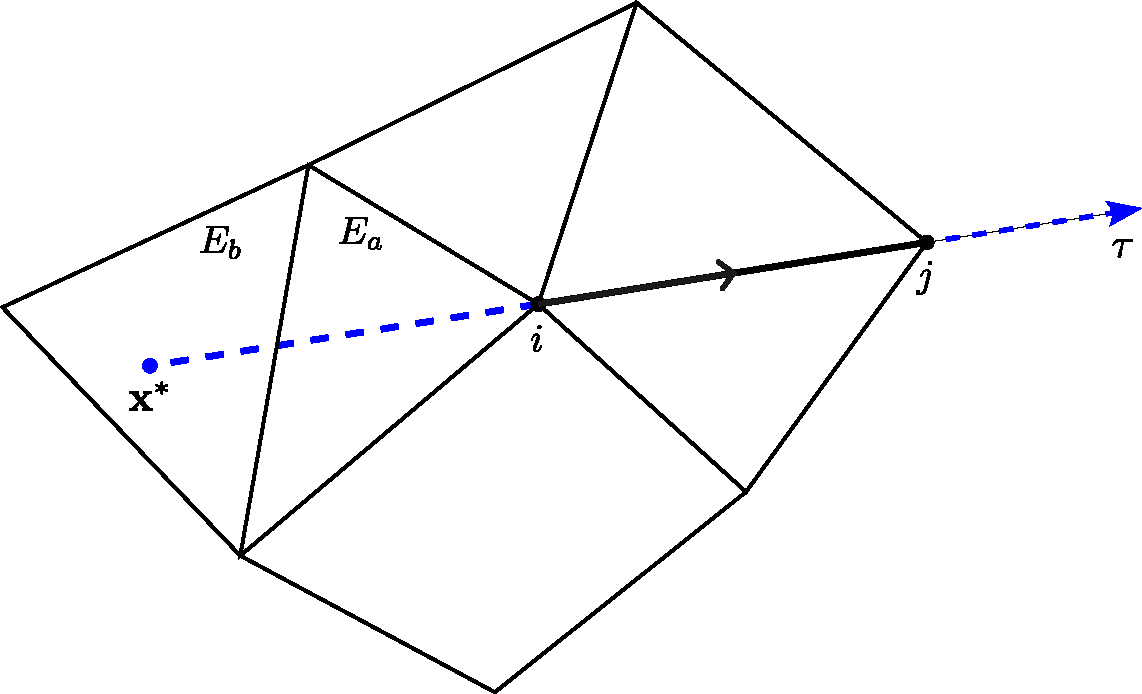
\includegraphics[width=0.7\linewidth]{fem_tvd_interpolation.pdf}
\caption{Вспомогательный узел $\vec x^*$ на конечноэлементной сетке}
\label{fig:fem_tvd_interpolation}
\end{figure}

\paragraph{Интерполяция/Экстраполяция в инцидентном элементе $E_a$}
Среди элементов, инцидентрых узлу $i$, найдём элемент $E_a$, ближайший к фиктивной точке $\vec x^*$.
Он может как содержать в себе эту фиктивную точку, так и не содержать (на \figref{fig:fem_tvd_interpolation} представлен второй случай).
Тогда можно записать
\begin{equation}
\label{eq:fem_tvd_interpolation_ea}
u_i - u(\vec x^*) = \sum_{k\in E_a} \phi^{(a)}_k(\vec x^*) (u_i - u_k).
\end{equation}
Подставляя это выражение в \cref{eq:fem_tvd_rij_nd} и далее в \cref{eq:fem_tvd_rijk} получим
\begin{equation*}
r^*_{ijk} = \phi_k^{(a)}(\vec x^*).
\end{equation*}
Для линейных конечных элементов значения элементных базисных функций справделиво:
\begin{equation*}
\phi^{(a)}(\vec x) = \begin{cases}
\in [0, 1],  &\quad \vec x \in E_a, \\
\notin [0, 1],  &\quad \vec x \notin E_a.
\end{cases}
\end{equation*}
Поэтому в случае экстраполяции возможно $r^*_{ijk} < 0$, поэтому такая схема не является монотонной по критерию Хартена.

\paragraph{Интерполяция в содержащем элементе $E_b$}
Теперь для интерполяции используем элемент, точно содержащий $\vec x^*$
независимо от того, является ли он инцидентным узлу $i$. Тогда аналогично
\begin{equation}
\label{eq:fem_tvd_interpolation_eb}
u_i - u(\vec x^*) = \sum_{k\in E_b} \phi^{(a)}_k(\vec x^*) (u_i - u_k).
\end{equation}
В этом случае в линейных элементов критерий Хартена удовлетворяется. Но терятся локальность схемы.

\paragraph{Использование градиента в узле $u_i$}
Воспользуемся методикой восстановления фиктивного значения $u^*$
из градиента, ранее рассмотренного для метода конечных объёмов \secref{sec:grad_inteprolate_up}.
Выделим ось $\tau$, последовательно содержащую узлы $\vec x^*$, $\vec x_i$, $\vec x_j$ на равном удалении.
Рассмотрим производную по этой оси в центральном узле $i$.
С одной стороны из односторонней разности
\begin{equation*}
\left.\dfr{u}{\tau}\right|_i = \frac{u_i - u^*}{|\vec x_i - \vec x^*|}.
\end{equation*}
С другой стороны согласно проекии общего вектора градиента
\begin{equation*}
\left.\dfr{u}{\tau}\right|_i = \left( \nabla u \right)_i \cdot \frac{\vec x_j - \vec x_i} {|\vec x_j - \vec x_i| }.
\end{equation*}
Пользуясь равноудалённостью узлов запишем искомую величину как
\begin{equation*}
u_i - u^* = \left( \nabla u \right)_i \cdot (\vec x_j - \vec x_i).
\end{equation*}
Далее определим градиент в узле с использованием МКЭ подхода.
Запишем уравнение.
\begin{equation*}
\vec g = \nabla u
\end{equation*}
Далее домножим на пробную функцию и разложим сеточные функции по базису. Тогда, с использованием
сосредоточенной матрицы масс получим
\begin{equation*}
\vec g_i = \frac{1}{m_i}\sum_k \vec c_{ik} u_k,
\end{equation*}
где градиентная матрица вычисляется по формуле
\begin{equation*}
\vec c_{ik} = \arint{\nabla \phi_k \, \phi_i}{\Omega}{\vec x}
\end{equation*}
Используя свойство согласованности базисных функций $\sum_j \phi_j = 1$
и формулу интегрирования по частям
\cref{eq:partint}
несложно получить два свойства
этой матрицы:
\begin{align}
& \sum_k \vec c_{ik} = 0,                                                  \label{eq:fem_tvd_cij_prop1}\\
& \vec c_{ik} = -\vec c_{ki}, \quad \text{для внутренних узлов $i$, $k$}. \label{eq:fem_tvd_cij_prop2}
\end{align}
С помощью первого из этих свойств \cref{eq:fem_tvd_cij_prop1}
можно записать искомое выражение
\begin{equation}
\label{eq:fem_tvd_interpolation_gradient}
u_i - u^* = \frac{1}{m_i}\sum_{k\neq i} \vec c_{ik} \cdot (\vec x_j - \vec x_i) (u_k - u_i).
\end{equation}
Откуда 
\begin{equation}
\label{eq:fem_tvd_gradient_rijk}
r^*_{ijk} = \frac{1}{m_i}\vec c_{ik} \cdot (\vec x_j - \vec x_i).
\end{equation}
Из свойства антисимметричности матрицы \cref{eq:fem_tvd_cij_prop2}
следует, что $\vec c_{ik}$ могут быть отрицательными.
Так же отрицательными могут быть компоненты вектора разности $\vec x_j - \vec x_i$.
Поэтому схема \cref{eq:fem_tvd_interpolation_gradient}
не удовлетворяет критерию монотонности.

\paragraph{Использование противопоточного градиента в узле $u_i$}
Для того, чтобы вписаться в требование монотоноости модифицируем
выражение \cref{eq:fem_tvd_interpolation_gradient},
оставив в нём только положительные коэффициенты.
Чтобы компенсировать отброшенные слагаемые умножим
полученное выражение на два:
\begin{equation}
\label{eq:fem_tvd_interpolation_upwind_gradient}
u_i - u^* = \frac{2}{m_i}\sum_{k\neq i} \max(0, \vec c_{ik} \cdot (\vec x_j - \vec x_i)) (u_k - u_i).
\end{equation}
\begin{equation}
Тогда
\label{eq:fem_tvd_upwind_gradient_rijk}
r^*_{ijk} = \frac{2}{m_i}\max(0, \vec c_{ik} \cdot (\vec x_j - \vec x_i)).
\end{equation}
Этот подход к построению противопотокового градиента
похож на построение оператора переноса
первого порядка точности с помощью алгебраической методики \cref{eq:fem_transport_dij} (см. схему 
\cref{eq:fem_tvd_matrices_1d} для одномерной аналогии).

\subsubsubsection{Алгебраический метод}
Запишем одномерный критерий TVD в виде:
\begin{equation}
r_{i,i+1} = \frac{k_{i,i-1} (u_{i-1} - u_{i})}{k_{i,i+1} (u_{i+1} - u_{i})}
\end{equation}

Наивное многомерное обобщение могло бы выглядеть так
\begin{equation}
r_{ij} = \frac
{\displaystyle\sum_k \max(0, k_{ik}) (u_{k} - u_{i})}
{\displaystyle\sum_k \min(0, k_{ik}) (u_{k} - u_{i})}
\end{equation}

Тогда
\begin{equation}
r^*_{ijk} = \frac{-\max(0, k_{ik}) (u_j - u_i)} {\displaystyle\sum_k \min(0, k_{ik}) (u_k - u_i)}
\end{equation}

Такое определение не гарантирует положительность $r^*_{ijk}$.
Необходимо, чтобы знаки $(u_j - u_i)$ и $(u_k - u_i)$ совпадали.
Заметим ещё одно свойство одномерной схемы:
в случае монотонного поведения $u_i$, знаки разностей $(u_{i+1} - u_i)$, $(u_{i-1} - u_i)$ в числителе и знаменателе различаются.
Причём знак в знаменателе совпадает со знаком текущего узла по потоку $j$ (который в одномерном случае равен $i+1$).
Тогда естественным обобщением выглядит
\begin{equation}
r_{ij} = \begin{cases}
\frac {\displaystyle\sum_k \max(0, k_{ik}) \min(0, (u_{k} - u_{i}))} {\displaystyle\sum_k \min(0, k_{ik}) \min(0, (u_{k} - u_{i}))}, &\quad u_i \geq u_j, \\[30pt]
\frac {\displaystyle\sum_k \max(0, k_{ik}) \max(0, (u_{k} - u_{i}))} {\displaystyle\sum_k \min(0, k_{ik}) \max(0, (u_{k} - u_{i}))}, &\quad u_i < u_j.
\end{cases}
\end{equation}

Окончательно запишем
\begin{equation}
\label{eq:fem_tvd_algebraic_rij}
r_{ij} = \begin{cases}
Q_i^+ / P_i^+, &\quad u_i \geq u_j,\\
Q_i^- / P_i^-, &\quad u_i \geq u_i,\\
\end{cases}
\end{equation}

\begin{align}
&Q_i^{\pm} = \sum_k \max(0, k_{ik})\substack{\max \\ \min} (u_k - u_i), \\
&P_i^{\pm} = \sum_k \min(0, k_{ik})\substack{\min \\ \max} (u_k - u_i).
\end{align}

Вспомитная строку $j$
\cref{eq:fem_tvd_fji}
окончательно запишем антидиффузию:
\begin{equation}
f_{ij} = f_{ji} = \min(\Phi(r_{ij}) d_{ij}, l_{ji})
\end{equation}

Алгоритм будет иметь такой вид
\begin{enumerate}
\item
Вычислить $k_{ij}$ -- сеточную матрицу переноса второго порядка,
\item
Вычислить линейную диффузию $d_{ij} = \max(0, -k_{ij}, -k_{ji})$.
\item
Вычислить $l_{ij} = k_{ij} + d_{ij}$
\item
Для каждого узла $i$ определить $Q^{\pm}_i$, $P^{\mp}_i$
\item
В цикле для напраленных граней $\overrightarrow{ij}$ определить $f_{ij}$
\item
окончательно собрать матрицу переноса с ограничением
$k^*_{ij} = k_{ij} + d_{ij} - f_{ij}$.
\end{enumerate}


%\section{Моделирирование течения вязкой несжимаемой жикости}
\subsection{Система уравнений Навье-Стокса}

Будем рассматривать стационарную двумерную систему уравнений
Навье-Стокса для вязкой несжимаемой жидкости.
В безразмерном консервативном виде в декартовой системе координат она имеет вид

\begin{align}
    \label{eq:ns2d_u}
    & \dfr{u^2}{x} + \dfr{uv}{y} =
        -\dfr{p}{x}
        + \frac{1}{\Ren}\left(\dfrq{u}{x} + \dfrq{u}{y}\right),\\[5pt]
    \label{eq:ns2d_v}
    & \dfr{uv}{x} + \dfr{v^2}{y} =
        -\dfr{p}{y}
        + \frac{1}{\Ren}\left(\dfrq{v}{x} + \dfrq{v}{y}\right), \\[5pt]
    \label{eq:ns2d_div}
    &\dfr{u}{x} + \dfr{v}{y} = 0.
\end{align}

Неизвестными являются поля скорости: $u$ -- в направлении оси $x$,
$v$ -- в направлении оси $y$, и давления $p$.

Число Рейнольдса определено через характерную скорость $U$, [м/c] и
характерный линейный размер $L$, [м] как
\begin{equation*}
    \Ren = \frac{UL\rho}{\mu},
\end{equation*}
где $\rho$, [кг/м$^3$] -- постоянная (вследствии несжимаемости) плотность жидкости, а
$\mu$, [Па$\cdot$с] -- динамическая вязкость жидоксти.

Характерое значение для давление выпишется в виде:
$ p^0 = \rho U^2 $, [Па].

Для решения этой системы будем использовать метод конечных разностей
с аппроксимацией по пространству второго порядка и последовательное (раздельное) решение входящих в неё
уравнений.

Глядя на вид уранений \cref{eq:ns2d_u,eq:ns2d_v,eq:ns2d_div}
можно выделить несколько проблем, которые необходимо решить
при построении расчётной схемы:
\begin{itemize}
\item нелинейность конвективного оператора в \eqref{eq:ns2d_u}, \eqref{eq:ns2d_v},
\item отсутствие явного уравнения для определения давления,
\item аппркосимация первых производных для давления и скорости со вторым порядком точности.
\end{itemize}


Для решения первой проблемы будем использовать итерационный процесс с линеаризацией -- то есть
записывать уравнение на итерационном слое используя значения неизвестных полей с прошлого слоя.
Вторую проблему будем решать с помощью алгоритма SIMPLE
связывания давления и скорости (Pressure-Velocity Coupling).

\subsection{Схема расчёта SIMPLE}
\label{sec:simple_scheme}

\subsubsection{Линеаризация}
Для избавления от нелинейности по скорости в системе \cref{eq:ns2d_u,eq:ns2d_div} в качестве скорости переноса будем
использовать значение с прошлой итерации.
Тогда задача на одном итерационном слое примет вид

\begin{align}
    \label{eq:ns2d_semi_u}
    & \dfr{u \hat u}{x} + \dfr{v \hat u}{y} =
        -\dfr{\hat p}{x}
        + \frac{1}{\Ren}\left(\dfrq{\hat u}{x} + \dfrq{\hat u}{y}\right),\\[5pt]
    \label{eq:ns2d_semi_v}
    & \dfr{u\hat v}{x} + \dfr{v \hat v}{y} =
        -\dfr{\hat p}{y}
        + \frac{1}{\Ren}\left(\dfrq{\hat v}{x} + \dfrq{\hat v}{y}\right), \\[5pt]
    \label{eq:ns2d_semi_div}
    &\dfr{\hat u}{x} + \dfr{\hat v}{y} = 0.
\end{align}

На итерационном слое значения $u, v, p$
известны, а $\hat u, \hat v, \hat p$ подлежат определению.

Критерием выхода из итерационного процесса является пороговое условие на невязку,
вычисленную с использованием найденных на слое значений неизвестных:
\begin{align}
    \nonumber
    &r_u = \dfr{\hat u \hat u}{x} + \dfr{\hat u \hat v}{y}
        + \dfr{\hat p}{x}
        - \frac{1}{\Ren}\left(\dfrq{\hat u}{x} + \dfrq{\hat u}{y}\right),\\[5pt]
    \nonumber
    &r_v = \dfr{\hat u\hat v}{x} + \dfr{\hat v \hat v}{y}
        +\dfr{\hat p}{y}
        - \frac{1}{\Ren}\left(\dfrq{\hat v}{x} + \dfrq{\hat v}{y}\right), \\[5pt]
    \label{eq:ns2d_residual}
    &\max(\lVert r_u \rVert, \lVert r_v \rVert) < \eps.
\end{align}

\subsubsection{Релаксация по скорости}
\label{sec:simple-algo}

В результате пространственной аппроксимации уравнений \cref{eq:ns2d_u}
получим матричную систему вида
\begin{align}
\nonumber
&\mat{A}^u \hat u = -\dfr{\hat p}{x}. \\[5pt]
\nonumber
&\mat{A}^v \hat v = -\dfr{\hat p}{y}.
\end{align}
Отметим, что хотя матрицы $\mat{A}^u$ и $\mat{A}^v$ получены в результате
аппроксимации одного и того же дифференциального оператора (конвекции и диффузии),
они могут различаться из-за особенностей аппроксимации.

Эта система при малых числах $\Ren$  не имеет диагонального преобладания
и неудобна для численного решения. Чтобы исправить этот недостаток
введём релаксацию по диагональному параметру с коэффициентом $\alpha_u$:
\begin{equation}
\label{eq:ns2d_linearized_u}
\frac{1}{\alpha_u} a^u_{ii}\hat u_i = -\sum_{j\neq i} a^u_{ij} \hat u_j -\dfr{\hat p}{x} + \frac{1 - \alpha_u}{\alpha_u} a^u_{ii} u_i
\end{equation}

\subsubsection{Связывание давления и скорости}
\label{sec:ns2d_segragated}
Приведём алгоритм для явного выражения уравнения для давления из
уравнения неразрывности \eqref{eq:ns2d_semi_div}.

Распишем искомые перенные в виде суммы 
\begin{equation}
    \label{eq:ns2d_decomp}
\begin{array}{l}
    \hat u = u^* + u',\\
    \hat v = v^* + v',\\
    \hat p = p + p'.
\end{array}
\end{equation}

Пусть введённое выше поле $u^*$ удовлетворяет уравнению
\begin{align}
    \label{eq:ns2d_ustar}
    &\frac{1}{\alpha_u} a^u_{ii} u^*_i = -\sum_{j\neq i} a^u_{ij} u^*_j - \dfr{p}{x} + \frac{1 - \alpha_u}{\alpha_u} a^u_{ii} u_i, \\[5pt]
    \label{eq:ns2d_vstar}
    &\frac{1}{\alpha_u} a^v_{ii} v^*_i = -\sum_{j\neq i} a^v_{ij} v^*_j - \dfr{p}{y} + \frac{1 - \alpha_u}{\alpha_u} a^v_{ii} v_i,
\end{align}

Тогда уравнение для поправки скорости запишем вычтя последнее выражение из
уравнения \eqref{eq:ns2d_linearized_u}:
\begin{align}
  \label{eq:ns2d_uprime}
  &\frac{1}{\alpha_u} a^u_{ii} u'_i = -\sum_{j\neq i} a^u_{ij} u'_j - \dfr{p'}{x}, \\[5pt]
  \label{eq:ns2d_vprime}
  &\frac{1}{\alpha_u} a^v_{ii} v'_i = -\sum_{j\neq i} a^v_{ij} v'_j - \dfr{p'}{y},
\end{align}

Основная идея алгоритма SIMPLE заключается в приближённом представлении выражения \eqref{eq:ns2d_uprime}
в явном виде относительно поправки. Для этого отбросим внедиагональные компоненты в матрице $\mat A$.
Тогда можно явно выразить поправку скорости как
\begin{equation}
    \label{eq:ns2d_uprime_approx}
    u'_i \approx -d^u_i \left(\dfr{p'}{x}\right)_i, \quad d^u_i = \frac{\alpha_u}{a^u_{ii}}
\end{equation}

Аналогичные рассуждения в отношении поправки поперечной скорости $v'$ приводят к выражению

\begin{equation}
    \label{eq:ns2d_vprime_approx}
    v'_i \approx -d^v_i \left(\dfr{p'}{y}\right)_i, \quad d^v_i = \frac{\alpha_u}{a^v_{ii}}
\end{equation}

Далее используем уравнение неразрывности \cref{eq:ns2d_semi_div}. Подставим
в него разложения \cref{eq:ns2d_decomp} и используем
\cref{eq:ns2d_uprime_approx,eq:ns2d_vprime_approx}.
Тогда
получим уравнение Пуассона с непостоянным по пространству векторным коэффициентом диффузии $\left(d^u, d^v\right)$
относительно поправки давления $p'$:
\begin{equation}
    \label{eq:ns2d_pprime_diff}
    -\left[
    \dfr{}{x}\left(
       d^u \dfr{p'}{x} 
            \right)
    +\dfr{}{y}\left(
       d^v \dfr{p'}{y} 
            \right)
    \right]
    =
    -\left(\dfr{u^*}{x} + \dfr{v^*}{y}\right).
\end{equation}

\subsubsection{Итерационный процесс}
Определим порядок вычислений на итерационном слое.
Напомним, что значения $u, v, p$ с
предыдущего слоя нам известно и задача
состоит в нахождении значений $\hat u, \hat v, \hat p$
на текущем слое.

\begin{enumerate}
\item Из уравнений \eqref{eq:ns2d_ustar}, \eqref{eq:ns2d_vstar}
      вычисляются значения $u^*, v^*$;
\item Они используются для вычисления правой части уравнения \eqref{eq:ns2d_pprime_diff},
      в результате решения которого находится поправка давления $p'$;
\item Дифференцируя найденную поправку давления найдём поправки скорости $u', v'$
      из выражений \eqref{eq:ns2d_uprime_approx}, \eqref{eq:ns2d_vprime_approx};
\item Окончательно выразим значения переменных для текущего слоя из \eqref{eq:ns2d_decomp}.
      Для улучшения стабильности алгоритма значение давления вычисляют
      с некоторым коэффициентом релаксации $\alpha_p$:
      \begin{equation*}
           \hat p = p + \alpha_p p';
      \end{equation*}
\item Далее проводится вычисление невязки с ипользованием найденных значений $\hat u, \hat v, \hat p$
      из выражения \eqref{eq:ns2d_residual}. Если она недостаточно мала,
      то выполняется присваивание
      $
           u = \hat u, \; v=\hat v, \; p = \hat p
      $ 
      и возвращение на шаг 1.
\end{enumerate}

Полученные на каждом шаге итерационного процесса компоненты скорости $\hat u, \hat v$
точно удовлетворяют уравнению неразрывности \eqref{eq:ns2d_semi_div}, но
уравнения движения \eqref{eq:ns2d_semi_u}, \eqref{eq:ns2d_semi_v} выполняются лишь приближённо.

Всего в алгоритме SIMPLE есть два параметра: коэффициент
релаксации давления $\alpha_p$ и коэффициент релаксации скорости $\alpha_u$.
Характерые значения для этих параметров:
\begin{equation*}
\alpha_u = 0.8, \quad \alpha_p = 0.3.
\end{equation*}

\subsection{Пространственная аппроксимация методом конечных разностей}
\label{sec:simple_scheme_fdm}

Для численной реализации алгоритма решения
необходимо провести пространственную аппроксимацию полудискретизованных
выражений
\eqref{eq:ns2d_ustar}, \eqref{eq:ns2d_vstar}, \eqref{eq:ns2d_uprime_approx},
\eqref{eq:ns2d_vprime_approx}, \eqref{eq:ns2d_pprime_diff}.

Для решения проблем с неустойчивостью схемы по давлению (checkboard instability)
проводить конечноразностную аппроксимацию будем на разнесённой сетке (Staggered Grid).

\subsubsection{Разнесённая сетка}

Будем использовать структурированную четырёхугольную сетку
с постоянным шагом по пространству.
При этом неизвестные параметры будем задавать
по схеме, представленной на \figref{fig:staggered_grid}.

\begin{figure}[h]
\centering
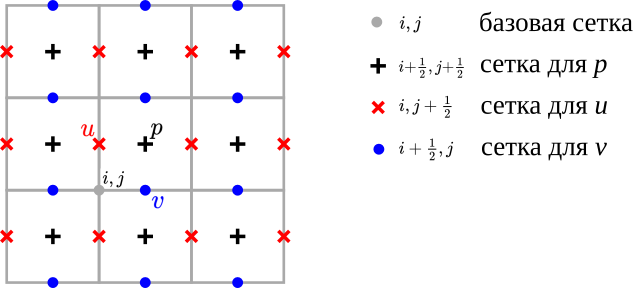
\includegraphics[width=0.6\linewidth]{staggered_grid.png}
\caption{Разнесённая сетка}
\label{fig:staggered_grid}
\end{figure}

Введём разбиение сетки:
$n_x$ -- количество ячеек в направлении $x$,
$n_y$ -- количество ячеек в направлении $y$.

Очевидно, что при использовании такого разнесённого шаблона,
количество точек, в которых заданы значения, будет
различным для разных параметров.
Так количество узловых значений давления будет равно $n_x \times n_y$,
продольной скорости $u$ -- $(n_x+1) \times n_y$, а поперечной $v$ -- $n_x \times (n_y+1)$.

Использование такого расположения узловых точек
даёт преимущество при аппроксимации
первых производных. Так, конечная разность
\begin{equation*}
\left.\dfr{p}{x}\right|_{i, j+\tfrac12} = \frac{p_{i+\tfrac12,j+\tfrac12} - p_{i-\tfrac12,j+\tfrac12}}{h_x} + o(h_x^2)
\end{equation*}
будем симметричной в узле $i,j+\tfrac12$, где задана
компонента скорости $u$, и поэтому будет иметь там второй порядок точности.

Выражения \eqref{eq:ns2d_ustar}, \eqref{eq:ns2d_uprime_approx} аппроксимируются
на сетке для $u$, выражения \eqref{eq:ns2d_vstar}, \eqref{eq:ns2d_vprime_approx} -- 
на сетке для $v$, а \eqref{eq:ns2d_pprime_diff} -- на сетке для $p$.

Введём сквозную линейную нумерацию узлов сетки: нулевой узел разположим в левом нижнем углу,
далее будем индексировать слева направа и потом снизу вверх.
Для основной сетки перевод двумерного индекса $i,j$ в сквозной индекс будет проводится по формуле
\begin{equation}
    \label{eq:ns2d_kij}
    k(i,j) = j(n_x+1)+i.
\end{equation}
Для сеток, на которых заданы сеточные параметры, такой перевод примет вид
\begin{align}
    \label{eq:ns2d_kipjp}
    &k(i+\tfrac12,j+\tfrac12) = jn_x + i, \quad - \; \text{сетка для давления } p\\[10pt]
    \label{eq:ns2d_kijp}
    &k(i,j+\tfrac12) = j(n_x+1) + i, \quad - \;  \text{сетка для продольной скорости } {\color{red} u} \\[10pt]
    \label{eq:ns2d_kipj}
    &k(i+\tfrac12,j) = jn_x + i, \quad - \; \text{сетка для поперечной скорости } {\color{blue} v}
\end{align}

\subsubsection{Уравнения движения}

Запишем конечноразностную аппроксимацию уравнения \eqref{eq:ns2d_ustar} для пробной скорости $u^*$ в ``красных'' узлах сетки
$\left(i, j+\tfrac12\right)$:

\begin{align}
    \label{eq:ns2d_ustar_discr}
       &\frac{1}{\alpha_u}\frac{2}{\Ren}\left(\frac{1}{h_x^2} + \frac{1}{h_y^2}\right)
          \left(u^*_{i,j+\tfrac12}\right)   \\[10pt]
    \nonumber
       &-\frac{1}{\Ren}\frac{1}{h_x^2}
          \left(
            u^*_{i-1,j+\tfrac12} + u^*_{i+1,j+\tfrac12}
          \right)
       -\frac{1}{\Ren}\frac{1}{h_y^2}
          \left(
            u^*_{i,j-\tfrac12} + u^*_{i,j+\tfrac32}
          \right)   \\[10pt]
    \nonumber
       &+\frac{1}{h_x}
          \left(
            \left(u u^*\right)_{i+\tfrac12,j+\tfrac12}-
            \left(u u^*\right)_{i-\tfrac12,j+\tfrac12}
          \right)
        +\frac{1}{h_y}
          \left(
            \left(v u^*\right)_{i,j+1}-
            \left(v u^*\right)_{i,j}
          \right)   \\[10pt]
    \nonumber
       =&\frac{1-\alpha_u}{\alpha_u}\frac{2}{\Ren}\left(\frac{1}{h_x^2} + \frac{1}{h_y^2}\right)
          \left(u_{i,j+\tfrac12}\right)   \\[10pt]
    \nonumber
       &-\frac{1}{h_x}\left(p_{i+\tfrac12,j+\tfrac12} - p_{i-\tfrac12,j+\tfrac12}\right).
\end{align}

В приведённом выражении
за исключением конвективных слагаемых вида $u u$ все остальные
сеточные вектора используются на своих сетках.
Конвективные слагаемые распишем через полусуммы вида:
\begin{equation*}
    u_{i+\tfrac12} = \frac{u_{i} + u_{i+1}}{2} + o(h^2)
\end{equation*}

Тогда
\begin{align*}
    \left(u u^*\right)_{i+\tfrac12,j+\tfrac12} =&
        \left(u_{i+\tfrac12,j+\tfrac12} \vphantom{u^*_{\tfrac12}}\right)\left(u^*_{i+\tfrac12,j+\tfrac12}\right) =
        \frac14 \left(u_{i, j+\tfrac12} + u_{i+1,j+\tfrac12}\vphantom{u^*_{\tfrac12}}\right)
                \left(u^*_{i, j+\tfrac12} + u^*_{i+1,j+\tfrac12}\right), \\[10pt]
    \left(u u^*\right)_{i-\tfrac12,j+\tfrac12} =&
        \frac14 \left(u_{i, j+\tfrac12} + u_{i-1,j+\tfrac12}\vphantom{u^*_{\tfrac12}}\right)
                \left(u^*_{i, j+\tfrac12} + u^*_{i-1,j+\tfrac12}\right), \\[10pt]
    \left(v u^*\right)_{i,j+1} =&
        \frac14 \left(v_{i+\tfrac12, j+1} + v_{i-\tfrac12,j+1}\vphantom{u^*_{\tfrac12}}\right)
                \left(u^*_{i, j+\tfrac32} + u^*_{i,j+\tfrac12}\right), \\[10pt]
    \left(v u^*\right)_{i,j} =&
        \frac14 \left(v_{i+\tfrac12, j} + v_{i-\tfrac12,j}\vphantom{u^*_{\tfrac12}}\right)
                \left(u^*_{i, j+\tfrac12} + u^*_{i,j-\tfrac12}\right).
\end{align*}

Схему \eqref{eq:ns2d_vstar}
можно записать в виде системы линейных уравнений вида
\begin{equation}
    \label{eq:ns2d_ustar_slae}
    \mat{A}^u u^* = b^{u},
\end{equation}
Сеточная матрица $A^u$ будет иметь $(n_x+1)n_y$ строк.
Для строки, соответствующей $\left(i,j+\tfrac12\right)$ узлу ненулевыми будут столбцы,
соответствующие узлам:
\begin{itemize}
\item $\left(i,j+\tfrac12\right)$,
\item $\left(i+1,j+\tfrac12\right)$,
\item $\left(i-1,j+\tfrac12\right)$,
\item $\left(i,j+\tfrac32\right)$,
\item $\left(i,j-\tfrac12\right)$.
\end{itemize}

В случае использования стандартной нумерации узлов структурированной сетки,
когда нулевой индекс соответствуют левому нижнему узлу и далее нумерация идёт
с быстрым индексом $i$, то матрица будет пятидиагональной.


Подставим полученные выражения в конвективную часть выражения \eqref{eq:ns2d_ustar_discr}.
Множитель при диагональном элементе $u^*_{i,j+\tfrac12}$ будет равен:
\begin{align*}
        \frac{1}{4}\Biggl(
         \underbrace{\frac{u_{i,j+\tfrac12} - u_{i-1,j+\tfrac12}}{h_x}}_{\left.\ddfr{u}{x}\right|_{i-\tfrac12,j+\tfrac12}}
        +\underbrace{\frac{u_{i+1,j+\tfrac12} - u_{i,j+\tfrac12}}{h_x}}_{\left.\ddfr{u}{x}\right|_{i+\tfrac12,j+\tfrac12}}
        +\underbrace{\frac{v_{i+\tfrac12,j+1} - v_{i+\tfrac12,j}}{h_y}}_{\left.\ddfr{v}{y}\right|_{i+\tfrac12,j+\tfrac12}}
        +\underbrace{\frac{v_{i-\tfrac12,j+1} - v_{i-\tfrac12,j}}{h_y}}_{\left.\ddfr{v}{y}\right|_{i-\tfrac12,j+\tfrac12}}
        \Biggr)
\end{align*}

Сумма первого и четвёртого слагаемых представляет собой разностный
аналог уравнения неразрывности \eqref{eq:ns2d_semi_div}, записанной для ``чёрного'' узла
сетки $i-\tfrac12, j+\tfrac12$ относительно компонент
скорости с предыдущей итерации.
Как было сказано ранее,
в настоящем алгоритме
уравнение неразрывности для итоговых по результатам итерации скорости в этих узлах выполняется точно.
Поэтому эта сумма в точности будет равна нулю. Аналогичный результат получится
и для суммы второго и третьего слагаемых. Отсюда следует вывод, что
конвективное слагаемое не даёт вклад в диагональ итоговой матрицы (как и следовало ожидать от симметричной аппроксимации).

Окончательно запишем все пять ненулевых вхождений в строку матрицы:
\begin{align}
    \label{eq:ns2d_au}
    \mat{A}^u\left[
        k\left(i,j+\tfrac12\right),
        k\left(i,j+\tfrac12\right)\right]
        &= \frac{1}{\alpha_u}\frac{2}{\Ren}\left(\frac{1}{h_x^2} + \frac{1}{h_y^2}\right)
        \quad - \;\text{основная диагональ}, \\[10pt]
    \nonumber
    \mat{A}^u\left[
        k\left(i,j+\tfrac12\right),
        k\left(i+1,j+\tfrac12\right)\right]
        &= -\frac{1}{\Ren}\frac{1}{h_x^2}
           +\frac{1}{4h_x}\left(u_{i,j+\tfrac12}+u_{i+1,j+\tfrac12}\right)
        \quad - \;\text{первая верхняя диагональ}, \\[10pt]
    \nonumber
    \mat{A}^u\left[
        k\left(i,j+\tfrac12\right),
        k\left(i-1,j+\tfrac12\right)\right]
        &= -\frac{1}{\Ren}\frac{1}{h_x^2}
           -\frac{1}{4h_x}\left(u_{i,j+\tfrac12}+u_{i-1,j+\tfrac12}\right)
        \quad - \;\text{первая нижняя диагональ}, \\[10pt]
    \nonumber
    \mat{A}^u\left[
        k\left(i,j+\tfrac12\right),
        k\left(i,j+\tfrac32\right)\right]
        &= -\frac{1}{\Ren}\frac{1}{h_y^2}
           +\frac{1}{4h_y}\left(v_{i+\tfrac12,j+1}+v_{i-\tfrac12,j+1}\right)
        \quad - \;\text{вторая верхняя диагональ}, \\[10pt]
    \nonumber
    \mat{A}^u\left[
        k\left(i,j+\tfrac12\right),
        k\left(i,j-\tfrac12\right)\right]
        &= -\frac{1}{\Ren}\frac{1}{h_y^2}
           -\frac{1}{4h_y}\left(v_{i+\tfrac12,j}+v_{i-\tfrac12,j}\right)
        \quad - \;\text{вторая нижняя диагональ}.
\end{align}
Правая часть аппроксимируется в виде
\begin{equation*}
    b^{u}[k(i, j+\tfrac12)] = - \frac{1}{h_x}\left(p_{i+\tfrac12,j+\tfrac12} - p_{i-\tfrac12,j+\tfrac12}\right)
        + \frac{1 - \alpha_u}{\alpha_u}\frac{2}{\Ren}\left(\frac{1}{h_x^2} + \frac{1}{h_y^2}\right) u_{i, j+\tfrac12}.
\end{equation*}
Здесь $k(i,j)$ -- функция перевода двумерного индекса в сквозной \eqref{eq:ns2d_kijp}.

Аналогичные выкладки для второго из уравнений движения \eqref{eq:ns2d_vstar}
дают систему уравнений
\begin{equation}
    \label{eq:ns2d_vstar_slae}
    \mat{A}^v v^* = b^{v},
\end{equation}
элементы пятидиагональной матрицы которой имеют вид
\begin{align}
    \label{eq:ns2d_av}
    \mat{A}^v\left[
        k\left(i+\tfrac12,j\right),
        k\left(i+\tfrac12,j\right)\right]
        &= \frac{1}{\alpha_u}\frac{2}{\Ren}\left(\frac{1}{h_x^2} + \frac{1}{h_y^2}\right)
        \quad - \;\text{основная диагональ}, \\[10pt]
    \nonumber
    \mat{A}^v\left[
        k\left(i+\tfrac12,j\right),
        k\left(i+\tfrac32,j\right)\right]
        &= -\frac{1}{\Ren}\frac{1}{h_x^2}
           +\frac{1}{4h_x}\left(u_{i+1,j+\tfrac12}+u_{i+1,j-\tfrac12}\right)
        \quad - \;\text{первая верхняя диагональ}, \\[10pt]
    \nonumber
    \mat{A}^v\left[
        k\left(i+\tfrac12,j\right),
        k\left(i-\tfrac12,j\right)\right]
        &= -\frac{1}{\Ren}\frac{1}{h_x^2}
           -\frac{1}{4h_x}\left(u_{i,j+\tfrac12}+u_{i,j-\tfrac12}\right)
        \quad - \;\text{первая нижняя диагональ}, \\[10pt]
    \nonumber
    \mat{A}^v\left[
        k\left(i+\tfrac12,j\right),
        k\left(i+\tfrac12,j+1\right)\right]
        &= -\frac{1}{\Ren}\frac{1}{h_y^2}
           +\frac{1}{4h_y}\left(v_{i+\tfrac12,j}+v_{i+\tfrac12,j+1}\right)
        \quad - \;\text{вторая верхняя диагональ}, \\[10pt]
    \nonumber
    \mat{A}^v\left[
        k\left(i+\tfrac12,j\right),
        k\left(i+\tfrac12,j-1\right)\right]
        &= -\frac{1}{\Ren}\frac{1}{h_y^2}
           -\frac{1}{4h_y}\left(v_{i+\tfrac12,j}+v_{i+\tfrac12,j-1}\right)
        \quad - \;\text{вторая нижняя диагональ}.
\end{align}
Правая часть аппроксимируется в виде
\begin{equation*}
    b^{v}[k(i+\tfrac12, j)] =  - \frac{1}{h_y}\left(p_{i+\tfrac12, j+\tfrac12} - p_{i+\tfrac12,j-\tfrac12}\right)
        + \frac{1 - \alpha_u}{\alpha_u}\frac{2}{\Ren}\left(\frac{1}{h_x^2} + \frac{1}{h_y^2}\right) v_{i, j+\tfrac12}.
\end{equation*}
Используется функция перевода двумерного индекса в сквозной из \eqref{eq:ns2d_kipj}.

\subsubsection{Уравнение для поправки давления}
Распишем уравнение \eqref{eq:ns2d_pprime_diff}
на ``чёрной'' сетке методом конечных разностей.
Для первого слагаемого получим
\begin{equation}
\label{eq:ns2d_d2pdx2}
\begin{array}{ll}
\left.\ddfr{}{x}\left(d^u \ddfr{p'}{x}\right) \right|_{i+\tfrac12, j+\tfrac12}
    &\approx
        \dfrac{1}{h_x}\left(
            d^u_{i+1, j+\tfrac12} \left. \ddfr{p'}{x} \right|_{i+1, j+\tfrac12} -
            d^u_{i, j+\tfrac12} \left. \ddfr{p'}{x} \right|_{i, j+\tfrac12}
        \right) \\[10pt]

    &=
        \dfrac{1}{h_x}\left(
            d^u_{i+1, j+\tfrac12} \dfrac{p'_{i+\tfrac32,j+\tfrac12} - p'_{i+\tfrac12,j+\tfrac12}}{h_x} - 
            d^u_{i, j+\tfrac12}  \dfrac{p'_{i+\tfrac12,j+\tfrac12} - p'_{i-\tfrac12,j+\tfrac12}}{h_x}
        \right).
\end{array}
\end{equation}
Коэффициенты $d^u$ и $d^v$ определяются для ``красной'' и ``синей'' сеток через диагональные значения матриц $\mat A$:
\begin{align}
\label{eq:ns2d_du_fdm}
d^u_{i,j+\tfrac12} =    \sfrac{1}{\mat{A}^u\left[
        k\left(i,j+\tfrac12\right),
        k\left(i,j+\tfrac12\right)\right]}, \\[5pt]
\label{eq:ns2d_dv_fdm}
d^v_{i+\tfrac12,j} =    \sfrac{1}{\mat{A}^v\left[
        k\left(i+\tfrac12,j\right),
        k\left(i+\tfrac12,j\right)\right]}.
\end{align}
Аналогично расписываются остальные слагаемые. В результате получим систему линейных уравнений вида
\begin{equation}
    \label{eq:ns2d_pprime_slae}
    A^p p' = b^p,
\end{equation}
где ненулевые коэффициенты пятидиагональной матрицы примут вид
\begin{align}
    \label{eq:ns2d_ap}
    A^p[k(i+\tfrac12, j+\tfrac12), k(i+\tfrac12, j+\tfrac12)] =&
        \frac{1}{h_x^2}\left( d^u_{i+1,j+\tfrac12} + d^u_{i,j+\tfrac12} \right)
        +\frac{1}{h_y^2}\left( d^v_{i+\tfrac12,j} + d^v_{i+\tfrac12,j+1} \right), \\[10pt]
    \nonumber
    A^p[k(i+\tfrac12, j+\tfrac12), k(i+\tfrac32, j+\tfrac12)] =&
        -\frac{1}{h_x^2}d^u_{i+1,j+\tfrac12}, \\[10pt]
    \nonumber
    A^p[k(i+\tfrac12, j+\tfrac12), k(i-\tfrac12, j+\tfrac12)] =&
        -\frac{1}{h_x^2}d^u_{i,j+\tfrac12}, \\[10pt]
    \nonumber
    A^p[k(i+\tfrac12, j+\tfrac12), k(i+\tfrac12, j+\tfrac32)] =&
        -\frac{1}{h_y^2}d^v_{i+\tfrac12,j+1}, \\[10pt]
    \nonumber
    A^p[k(i+\tfrac12, j+\tfrac12), k(i+\tfrac12, j-\tfrac12)] =&
        -\frac{1}{h_y^2}d^v_{i+\tfrac12,j}.\\[10pt]
\end{align}
Столбец свободных членов аппроксимируется в виде
\begin{equation}
    \label{eq:ns2d_bp}
    b^p[k(i+\tfrac12,j+\tfrac12)] = 
        -\left(
              \frac{u^*_{i+1,j+\tfrac12} - u^*_{i,j+\tfrac12}}{h_x}
            + \frac{v^*_{i+\tfrac12,j+1} - v^*_{i+\tfrac12,j}}{h_y}
        \right).
\end{equation}
Здесь используется функция перевода двумерного индекса в сквозной из $\eqref{eq:ns2d_kipjp}$.

В результате использования \eqref{eq:ns2d_du}, \eqref{eq:ns2d_dv} левая часть системы уравнений \eqref{eq:ns2d_pprime_slae}
будет постоянна на всех итерациях, что удобно для инициализации алгебраических решателей этой системы
(можно провести инициализацию один раз до начала счёта).

Это отличает эту систему от двух других систем, возникающих
из аппроксимации уравнений движения \eqref{eq:ns2d_ustar_slae}, \eqref{eq:ns2d_vstar_slae},
левые части которых зависят от значений с предыдущих
итерационных слоёв. Этот момент обуславливает выбор
решателей для этих систем, которые в эффективных гидродинамических кодах обычно
отличаются, от решателя для системы \eqref{eq:ns2d_pprime_slae}.


\subsubsection{Уравнение для поправки скорости}
И наконец рассмотрим аппроксимацию выражений \eqref{eq:ns2d_uprime_approx},
\eqref{eq:ns2d_vprime_approx}, которые примут явный вид
\begin{align}
    \label{eq:ns2d_uprime_discr}
    u'_{i,j+\tfrac12} = -d^u_{i,j+\tfrac12} \frac{p'_{i+\tfrac12,j+\tfrac12} - p'_{i-\tfrac12, j+\tfrac12}}{h_x}, \\[10pt]
    \label{eq:ns2d_vprime_discr}
    v'_{i+\tfrac12,j} = -d^v_{i+\tfrac12,j} \frac{p'_{i+\tfrac12,j+\tfrac12} - p'_{i+\tfrac12, j-\tfrac12}}{h_x}.
\end{align}

\subsubsection{Учёт граничных условий}
\label{sec:simple-bc}

Для уравнений Навье-Стокса на каждой границе расчётной области
требуется столько условий, сколько есть уравнений движения.
Для двумерной задачи \cref{eq:ns2d_u,eq:ns2d_div,eq:ns2d_v}
нужно задать два граничных условия.

При использовании разнесённой сетки граница области проходит
по граням основной сетки. 
На нижней и верхней границах расчётной области
присутствуют узлы для $v$, но отсутствуют
узлы для $u$.
На правой и левой границах, наоборот,
есть узлы с заданными компонентами $u$,
но нет узлов с компонентами $v$.
Узловые значения для давления $p$
никогда не бывают граничными.

Для простоты пока будем рассматривать только случай с заданными значениями
двух компонент скорости на каждой из границ задачи:
\begin{align*}
    &\left. u(x, y) \right|_{x,y\in\Gamma} = u^\Gamma(x, y), \\
    &\left. v(x, y) \right|_{x,y\in\Gamma} = v^\Gamma(x, y).
\end{align*}

В схеме SIMPLE частные граничные условия 
для скорости учитываются при решении задачи
для пробных скоростей $u^*, v^*$.
Тогда для поправки скорости $u', v'$ на границах
будут справедливы соответствующие однородные граничные условия (нулевые значения в нашем случае):

\begin{align}
    \label{eq:ns2d_usplit_bc}
    &\left. u^*(x, y) \right|_{x,y\in\Gamma} = u^\Gamma(x, y), \\
    \nonumber
    &\left. v^*(x, y) \right|_{x,y\in\Gamma} = v^\Gamma(x, y), \\
    \nonumber
    &\left. u'(x, y) \right|_{x,y\in\Gamma} = 0,\\
    \nonumber
    &\left. v'(x, y) \right|_{x,y\in\Gamma} = 0.
\end{align}

Для учёта граничных условий по скорости требуется модифицировать
системы линейных уравнений \eqref{eq:ns2d_ustar_slae}, \eqref{eq:ns2d_vstar_slae}.

Рассмотрим нижнюю границу $j=0$.

На нижней границе явно присутствуют узлы ``синей'' сетки.
Значит можно явно установить значения для скорости $v$
путём постановки нулей с единицой на диагонали в строке матрицы и отнесением необходимого
граничного значение в правый вектор столбец системы \eqref{eq:ns2d_vstar_slae}:
\begin{align}
    \label{eq:ns2d_bc1}
    &A^v[k(i+\tfrac12, 0), s] = \delta_{ks}, \quad \forall i, \; \forall s\\[10pt]
    \nonumber
    &b^{v}[k(i+\tfrac12, 0)] = v^\Gamma.
\end{align}
Такая модификация просто заменяет $k(i+\tfrac12, 0)$ -ое уравнение
системы \eqref{eq:ns2d_vstar_slae} на выражение
\begin{equation*}
    v^*_{i+\tfrac12, 0} = v^\Gamma.
\end{equation*}

Узлов для компонет $u$ на нижней границе нет.
Рассмотрим первый ряд точек ``красной'' сетки: $(i, \tfrac12)$.
Если бы мы захотели заполнить коэффициенты системы
линейных уравнений \eqref{eq:ns2d_ustar_slae}
по выведенным выше формулам \eqref{eq:ns2d_au}
для узла, расположенного в этом ряду, мы бы столкнулись
с необходимостью установки значения в фиктивную колонку:
последнее из уравнений \eqref{eq:ns2d_au}
предписывает нам установить значение по адресу
$[k(i, \tfrac12), k(i, -\tfrac12)]$, который, очевидно, не присутствует в матрице.

Действительно, $k(i,\tfrac12)$-ая строка системы уравнений \eqref{eq:ns2d_au}
имеет вид
\begin{equation}
    \label{eq:ns2d_au_low}
      D    u^*_{i, \tfrac12}
    + U^1  u^*_{i+1, \tfrac12}
    + L^1  u^*_{i-1, \tfrac12}
    + U^2 u^*_{i, \tfrac32}
    + L^2 u^*_{i, -\tfrac12} 
    = b^u_{i, \tfrac12},
\end{equation}
где $D$ -- коэффициент с основной диагонали, $U^{1,2}, L^{1,2}$ -- 
коэффициенты с двух верхних и двух нижних диагоналей, вычисляемые по формулам \eqref{eq:ns2d_au}.
Вторая нижняя диагональ у этой строки матрицы отсутствует.
Она соответствует вкладу от узла $(i, -\tfrac12)$, который лежит вне области расчёта, на полшага ниже
нижней границе.

Тем не менее, такой фиктивный узел мы можем 
использовать для записи аппроксимации
\begin{equation*}
    u^*_{i,0} = u^\Gamma = \frac{u^*_{i,\tfrac12} + u^*_{i, -\tfrac12}}{2} + o(h_x^2).
\end{equation*}
или
\begin{equation*}
    u^*_{i, -\tfrac12} \approx 2u^\Gamma - u^*_{i,\tfrac12}.
\end{equation*}

Подставляя это выражение в строку \eqref{eq:ns2d_au_low} получим
\begin{equation*}
      (D - L^2) u^*_{i, \tfrac12}
    + U^1       u^*_{i+1, \tfrac12}
    + L^1       u^*_{i-1, \tfrac12}
    + U^2       u^*_{i, \tfrac32}
    = b^u_{i, \tfrac12} + 2 u^\Gamma.
\end{equation*}

Таким образом, добавление коэффициента в фиктивную колонку строки матрицы при
наличие условия первого рода на границе равносильно
вычитанию этого коэффициента из диагонального элемента этой строки
и вычитанием удвоенного граничного значения из правой части.
В случае нижней границы получим
\begin{align}
    \label{eq:ns2d_bc2}
    &A^u[k(i, \tfrac12), k(i, \tfrac12)] \mathrel{-}= A^u[k(i, -\tfrac12)], \\[10pt]
    \nonumber
    &b^u[k(i, \tfrac12)] \mathrel{-}= 2 u^\Gamma.
\end{align}

Приёмы \eqref{eq:ns2d_bc1}, \eqref{eq:ns2d_bc2}
используются и на остальных границах для
постановки граничных условий для скорости.

При сборке системы линейных уравнений для
поправки давления \eqref{eq:ns2d_pprime_slae}
так же возникает проблема с обращением
к фиктивным узлам. Например, при рассмотрении левой стенки ($i=0$
третье из уравнений \eqref{eq:ns2d_ap} описывает
несуществующий столбец $k(-\tfrac12, j+\tfrac12)$.
Если обратиться к выражению \eqref{eq:ns2d_d2pdx2},
то будет видно, что это слагаемое пришло в результате
расписывания граничной производной $p'$,
которая, исходя из выражения \eqref{eq:ns2d_uprime_approx} пропорциональна граничному значению $u'$,
то есть, вспоминая \eqref{eq:ns2d_usplit_bc}, равна нулю:
\begin{equation*}
\left. \dfr{p'}{x} \right|_{0,j+\tfrac12} = -\frac{1}{d^u} u'_{0,j+\tfrac12} = 0.
\end{equation*}

То есть добавлять слагаемые, соответствующие фиктивным узлам, в матрицу $A^p$ не нужно.
Не нарушая общности выведённых ранее выражений \eqref{eq:ns2d_ap},
просто модифицируем значения коэффициентов $d^u, d^v$:
\begin{align}
    \label{eq:ns2d_bc3}
    d^u_{0, j+\tfrac12} = d^u_{n_x+1, j+\tfrac12} = 0, \\[10pt]
    \nonumber
    d^v_{i+\tfrac12, 0} = d^u_{i+\tfrac12, n_y+1} = 0.
\end{align}

В исходных уравнениях
\eqref{eq:ns2d_u}-\eqref{eq:ns2d_div}
давление присутствует только в виде своих производных.
Если в задаче нигде не задано явное граничное условие
для давления, то решение для давления
будет определено только с точностью до константы.
Чтобы убрать эту неопределённость
рекомендуется явно положить давление нулю
в любом узле. Например, в случае нулевого узла,
по аналогии с \eqref{eq:ns2d_bc1} запишем:
\begin{align}
    \label{eq:ns2d_bc4}
    &A^p[k(\tfrac12, \tfrac12), s] = \delta_{ks}, \\[10pt]
    \nonumber
    &b^{p}[k(\tfrac12, \tfrac12)] = 0.
\end{align}

\subsection{Пространственная аппроксимация методом конечных объёмов}
\label{sec:simple_scheme_fem}
В методе конечных объёмов узлами коллокации служат
центры ячеек, поэтому бороться с шахматными осцилляциями
путём разнесения узлов коллокации для разных
расчётных полей (разнесённая сетка) нельзя.
Вместо этого в набор искомых полей решения добавляется
нормальная к грани скорость течения, определённая для центров граней (между $i$-ой и $j$-ой точками коллокаций): $\unij$.
Для её нахождения используется специальный алгоритм Rhie--Chow, учитывающий текущее давления.
Кроме того отдельно вычисляется градиент давления в центрах ячеек $(\nabla p)_i$.

\subsubsection{Определяющие соотношения}
Запишем конечнообъёмную аппроксимацию линеаризованного уравнения сохранения импульса (аналог \cref{eq:ns2d_linearized_u}):
\begin{equation}
\label{eq:ns2d_fvmsimple_momentum}
\frac{1}{\alpha_u} a_{ii}\hat{\vec u_i} = -\sum_{j\neq i} a_{ij} \hat{\vec u_j} - m_i \left(\nabla \hat p\right)_i + \frac{1 - \alpha_u}{\alpha_u} a_{ii} \vec u_i.
\end{equation}
Здесь $m_i$ -- элемент матрицы масс, равный объёму ячейки $|E_i|$.
Далее следуя методике \secref{sec:ns2d_segragated}
подставим в него разложение \cref{eq:ns2d_decomp}
и запишем аналоги уравнений для пробной скорости \cref{eq:ns2d_ustar,eq:ns2d_vstar}:
\begin{equation}
\label{eq:ns2d_fvm_ustar}
\frac{1}{\alpha_u} a_{ii} \vec u^*_i = -\sum_{j\neq i} a_{ij} \vec u^*_j - m_i (\nabla p)_i + \frac{1 - \alpha_u}{\alpha_u} a_{ii} \vec u_i,
\end{equation}
и поправки \cref{eq:ns2d_uprime_approx,eq:ns2d_vprime_approx}:
\begin{equation}
\label{eq:ns2d_fvm_uprime}
\vec u' \approx - d \nabla{p'}, \quad d_i = \frac{\alpha_u m_i}{a_{ii}}.
\end{equation}
Отметим, что в случае, если диагонали матриц для
разных компонент скорости отличаются (например из-за нелинейных аппроксимаций конвекции),
то коэффициент $d$ является векторным.
Далее возьмём дивергенцию последнего выражения и воспользуемся уравнением неразрывности. Тогда
Получим уравнение для поправки давления
\begin{equation}
\label{eq:ns2d_fvm_prime}
-\nabla\cdot \left( d \nabla{p'}\right) = -\nabla \cdot \vec u^*.
\end{equation}

\subsubsection{Поправка Rhie--Chow}
\label{sec:rhie_chow}
Ключевым моментов алгоритма является конечнообъёмная аппроксимация правой части уравнения
\cref{eq:ns2d_fvm_prime}:
\begin{equation}
\label{eq:ns2d_fvm_div_ustar}
\arint{\nabla\cdot \vec u^*}{E_i}{\vec x} = \sum_{j\in I^i} \unij^* |\gamma_{ij}|.
\end{equation}
Вычисление нормальной скорости на грани по наивной формуле приведёт к шахматным осцилляциям. То есть
\begin{equation*}
\unij^* \neq \frac{\vec u^*_i + \vec u^*_j}{2} \vec n_{ij}.
\end{equation*}
Вместо этого выразим $u^*$ из соотношения \cref{eq:ns2d_fvm_ustar}:
\begin{equation}
\label{eq:ns2d_fvm_ustar2}
\vec u^* = \tilde{\vec u} - d (\nabla p), \qquad
\tilde{\vec u}_i = -\frac{\alpha_u}{a_{ii}}\sum_{j\neq i} a_{ij} \vec u^*_j + \left(1 - \alpha_u\right) \vec u_i.
\end{equation}
Далее спроецируем это выражение на нормаль к грани $\gamma_{ij}$:
\begin{equation*}
\unij^* = \left(\tilde u_n\right)_{ij} - d_{ij} \left(\dfr{p}{n}\right)_{ij}.
\end{equation*}
Для определения $\tilde\unij$ воспользуемся полусуммой
\begin{equation}
\label{eq:ns2d_fvm_utilde_n}
\left(\tilde u_n\right)_{ij} = \frac{\tilde{\vec u}_i + \tilde{\vec u}_j}{2} \cdot \vec n_{ij},
\end{equation}
каждое слагаемое которого распишем с помощью первого из выражений \cref{eq:ns2d_fvm_ustar2}. Окончательно получим
\begin{equation}
\label{eq:ns2d_fvm_unij_star}
\unij^* = \frac12\left(\vec u^*_i + \vec u^*_j\right) \cdot \vec n_{ij} + \frac12\left(d_i(\nabla p)_i + d_j(\nabla p)_j - 2 d_{ij}\left(\nabla p\right)_{ij} \right) \cdot \vec n_{ij}.
\end{equation}
Коэффициент $d_{ij}$ вычисляется простой полусуммой.
\begin{equation*}
d_{ij} = \frac{d_i + d_j}{2}.
\end{equation*}
Узловые значения градиентов $\left(\nabla p)\right)_{i}$ вычисляются
специальной процедурой на основе метода Гаусса (\secref{sec:fvm_gauss_grad}),
a то же значение на грани определяется классической конечно-разностной схемой
\begin{equation*}
\left(\dfr{p}{n}\right)_{ij} \approx \frac{p_j - p_i}{h_{ij}} + \text{Skew}.
\end{equation*}
Это же выражение используется для определения
нормальных комонент поправки скорости на основе формулы \cref{eq:ns2d_vprime_approx}:
\begin{equation}
\label{eq:ns2d_fvm_unij_prime}
\unij' = -d_{ij} \frac{p'_j - p'_i}{h_{ij}} + \text{Skew}.
\end{equation}
\subsubsection{Порядок вычислений на SIMPLE итерации}
\label{sec:fvm_simple_steps}
На начало итерационного шага нам известны
\begin{itemize}
\item узловые значения скорости $\vec u$,
\item узловые значения давления $p$,
\item узловые значения градиента давления $(\nabla p)_i$,
\item нормальные скорости на гранях $\unij$.
\item
В случае решения нестационарной задачи также известно
значение скорости с предыдущего временного слоя $\check{\vec u}$.
\end{itemize}
\begin{enumerate}
\item собираем определяющие матрицы $A$, используемые в выражениях \cref{eq:ns2d_fvmsimple_momentum}.
Для аппроксимации конвективного слагаемого в качестве скорости переноса используям значения $\unij$.
На этом шаге можно подставить в эту матрицу значения с предыдущих итераций и подсчитать невязку.
Если она достаточно мала, можно выходить из итераций.
\item Из диагонали полученной матрицы выписываем вектор $d_i$ по формуле \cref{eq:ns2d_vprime_approx}.
      Отметим, что если диагонали матрицы $A$ для компонент скорости различаются, то получим два (или три для 3D)
      таких вектора.
\item по второй из формул \cref{eq:ns2d_fvm_uprime},
      собираем правую часть и решаем уравнение \cref{eq:ns2d_fvmsimple_momentum} для нахождения $\vec u^*$.
\item собираем пробные потоки $\unij^*$ по формуле \cref{eq:ns2d_fvm_unij_star}
\item Решаем уравнение \cref{eq:ns2d_fvm_prime} и находим $p'$. Правую часть считаем по \cref{eq:ns2d_fvm_div_ustar}.
\item По методике (\secref{sec:fvm_gauss_grad}) вычисляем узловые значения градиента поправки давления $\left(\nabla p'\right)_i$.
\item Считаем поправку скорости $\vec u'$ по \cref{eq:ns2d_vprime_approx}.
\item Считаем нормальную компоненту поправки скорости $\unij'$ по \cref{eq:ns2d_fvm_unij_prime}
\item Обнвляем значения на итерации:
\begin{align*}
&\hat{\vec u} = \vec u^* + \vec u' \\
&\hat\unij = \unij^* + \unij'\\
&\hat p = p + \alpha_p p' \\
&(\nabla \hat p)_i = (\nabla p)_i + \alpha_p (\nabla p')_i.
\end{align*}
\end{enumerate}

\subsection{Модификации метода SIMPLE}
\subsubsection{SIMPLEC}

\subsubsection{SIMPLER}

\subsubsection{PISO}
\label{sec:fvm_piso_steps}
Идея метода состоит в том, чтобы решить
линеаризованную полудискретизованную систему уравнений Навье-Стокса
за одну SIMPLE итерацию.
Он не использует сглаживаний: $\alpha_p = \alpha_u = 1$.
Диагональное преобладание матрицы $A$ обеспечивается за счёт нестационарного слагаемого
$$\dfr{u}{t} \approx \frac{\hat u - \check u}{\dt}. $$
с достаточно малым шагом по времени $\dt$.
То есть этот метод подходит либо для нестационарных задач,
либо для стационарных задач, чьё решение ищется методом установления.

Вместо декомпозиции \cref{eq:ns2d_decomp}
используем более глубокое разложение
\begin{equation}
    \label{eq:ns2d_piso_decomp}
\begin{array}{l}
    \hat{\vec u} = \vec u^* + \vec u' + \vec u'' + \vec u''' + \dots + \vec u^{(k)},\\
    \hat p = p + p' + p'' + p''' + \dots + \vec p^{(k)}.
\end{array}
\end{equation}
Подставим его в исходное уравнение
моментов
\cref{eq:ns2d_fvmsimple_momentum}.
Итоговое уравнение разобьъём слудующим образом
\begin{equation}
\label{eq:ns2d_piso_momentum}
\begin{array}{llll}
\frac{1}{\alpha_u} a_{ii} \vec u^*_i = &-\sum_{j\neq i} a_{ij} \vec u^*_j &- m_i (\nabla p)_i  &+ \frac{1 - \alpha_u}{\alpha_u} a_{ii} \vec u_i + \frac{m_i}{\dt}\check{\vec u}_i, \\[10pt]
\frac{1}{\alpha_u} a_{ii} \vec u'_i  = &                                  &- m_i (\nabla p')_i &\\[10pt]
\frac{1}{\alpha_u} a_{ii} \vec u''_i = &-\sum_{j\neq i} a_{ij} \vec u'_j   &- m_i (\nabla p'')_i &\\[10pt]
\dots &&&\\[10pt]
\frac{1}{\alpha_u} a_{ii} \vec u^{(k)}_i =&-\sum_{j\neq i} a_{ij} \vec u^{(k-1)}_j &- m_i (\nabla p^{(k)})_i &\\[10pt]
\end{array}
\end{equation}
Мы по прежнему используем факторы релаксаций сохраняя общность обозначений с исходным SIMPLE алгоритмом и имея ввиду, что для PISO $alpha_u = alpha_p = 1$.
Кроме того такая записть будет использована в следующей модификации PIMPLE.

Уравнение неразрывности удовлетворим в виде:
\begin{equation}
\label{eq:ns2d_piso_incomp}
\nabla \cdot \vec u^* = -\nabla \cdot \vec u', \quad \nabla \cdot \vec u'' = 0, \quad ... \quad \nabla \cdot \vec u^{(k)} = 0.
\end{equation}


Первые два уравнения из \cref{eq:ns2d_piso_momentum} решаются полностью аналогично SIMPLE методике.
Поэтому на каждом временном шаге сначала выполним 
все шаги из алгоритма \label{ref:fvm_simple_steps}.
При этом в качестве начального приближения возьмём значения с предыдущего временного слоя.
Далее будем вычислять последовательные приближения искомых параметров в цикле PISO:
\begin{enumerate}
\item Пусть мы находимся на $k$ шаге PISO итерации и значения $u^{(k-1)}$, $p^{(k-1)}$ нам известны.
\item Применим к последнему из уравнений \cref{eq:ns2d_piso_momentum} оператор дивергенции.
      С учётом \cref{eq:ns2d_piso_incomp} выпишем и решим уравнение для поправки давления
\begin{equation*}
- \nabla \cdot \left(d \nabla p^{(k)} \right) = -\nabla\cdot \tilde{\vec u}, \quad \tilde{\vec u}_i = -\frac{d_i}{m_i}\sum_{j\neq i} a_{ij} \vec u^{(k-1)}_j.
\end{equation*}
Для вычисления значений на грани промежуточной скорости $\tilde{\vec u}$ воспользуемся простой формулой \cref{eq:ns2d_fvm_utilde_n}.
\item Определяем узловые значения градиента $(\nabla p^{(k)})_i$.
\item Далее из того же уравнения выразим значение текущей поправки
\begin{equation*}
\vec u^{(k)}_i = \tilde{\vec u}_i - d_i (\nabla p^{(k)})_i.
\end{equation*}
\item И её нормальную компоненту на грани
\begin{equation*}
\unij^{(k)} = \left(\tilde{u_n}\right)_{ij} - d_{ij} (\nabla_n p^{(k)})_{ij}.
\end{equation*}
\item Обнвляем итоговые значения
\begin{align*}
&\hat{\vec u} \pluseq \vec u^{(k)} \\
&\hat\unij \pluseq \unij^{(k)}\\
&\hat p \pluseq \alpha_p p^{(k)} \\
&(\nabla \hat p)_i \pluseq \alpha_p (\nabla p^{(k)})_i.
\end{align*}
\item Выход из PISO цикла осуществляется при
удовлетворении линеаризованного (скорость переноса с прошлого временного слоя) уравнения моментов
с заданной погрешностью.
\end{enumerate}

\subsubsection{PIMPLE}
\label{sec:fvm_pimple_steps}
Это метод объединяет в себя итерации SIMPLE \secref{sec:fvm_simple_steps},
каждая из которых дополняется итерационным циклом PISO \secref{sec:fvm_piso_steps}.
В отличии от чистого PISO
здесь можно использовать релаксации $\alpha_u, \alpha_p < 1$.
При этом мониторинг сходимости следует делать в первую очередь
для цикла верхнего уровня. Цикл PISO можно отграничить 2-3 уточняющими итерациями.

По сравнению с PISO метод PIMPLE более устойчив и допускает использования больших шагов по времени (и даже решение стационарных задач).
Кроме того по итогу временного слоя по PIMPLE исполняется исходное (нелинеаризованное) уравнение импульса.


%\section{Упрощенный учёт сжимаемости}
\subsection{Учёт теплового расширения. Гипотеза Буссинеска}

\subsection{Схемы с искусственной сжимаемостью}

\subsection{Многофазное течение. Модель Эйлер--Эйлер}
Рассмотрим несколько несжимаемых фаз $k=0,1,\dots$ в одном потоке.
Каждай фаза имеет свою вязкость $\mu_k$, постоянную плотность $\rho_k = \const$
и объёмную концентрацию $\phi_k \in [0, 1]$.
\begin{equation}
\label{eq:euler-euler-unitsum}
\sum_k \phi_k = 1.
\end{equation}
Для каждой фазы будут справедливы закон сохранения импульса и закон сохранения массы:
\begin{align}
\label{eq:euler-euler-mom}
&\frac{\partial (\phi_k \rho_k \mathbf{u}_k)}{\partial t} + \nabla \cdot (\phi_k \rho_k \mathbf{u}_k \mathbf{u}_k) = 
-\phi_k \nabla p + \nabla \cdot (\phi_k \boldsymbol{\tau}_k) + \mathbf{M}_k + \phi_k \rho_k \mathbf{g}, \\
\label{eq:euler-euler-mass}
&\dfr{\rho_k \phi_k}{t} + \nabla\cdot\left(\rho_k \phi_k \vec u_k\right) = 0,
\end{align}
где \(\boldsymbol{\tau}_k = \mu_k\left(\nabla\vec u + \nabla^T \vec u\right)\) — тензор вязких напряжений для фазы \(k\),
а $\vec M_k$ -- силы межфазного взаимодействия, действующие на фазу $k$.

\subsubsection{Модель сопротивления дисперсной фазы}
\label{sec:schiller-naumann}
Такая модель не учитывает жёсткую границу между фазами и допускает взаимопроникновение фаз
в одной единице объёма. Поэтому с её помощью часто считают мелкодисперсные системы.
Основной силой межфазного взаимодействия в этом случае будет сила сопротивления
дисперсных фаз ($k>0$) несущей фазе ($k=0$).
Для дисперсных фаз сила сопротивления запишется в виде
\[
\vec M_k = \frac{3}{4} \phi_k \rho_0 \frac{C_D}{d_k} 
|\mathbf{u}_0 - \mathbf{u}_k| (\mathbf{u}_0 - \mathbf{u}_k),
\]
где коэффициент сопротивления \(C_D\) определяется по корреляции Шиллера–Неймана через характерный размер дисперсной частицы $d_k$:
\[
C_D = 
\begin{cases}
\dfrac{24}{Re_k} \left(1 + 0.15\, Re_k^{0.687}\right), & Re_k \le 800, \\[10pt]
0.44, & Re_k > 800,
\end{cases}
\]
\[
Re_k = \frac{\rho_0 |\mathbf{u}_0 - \mathbf{u}_k| d_k}{\mu_0}.
\]
Для несущей фазы:
\[
\vec M_0 = -\sum_{k>0} \vec M_k.
\]

\subsubsection{Схема решения SIMPLE}
\label{sec:euler-euler-simple}
В случае несжимаемых фаз уравнения сохранения масс \cref{eq:euler-euler-mass} упростятся
до уравнений для $\phi_k$:
\begin{equation}
\label{eq:euler-euler-phi}
\dfr{\phi_k}{t} + \nabla\cdot\left(\phi_k \vec u_k\right) = 0,
\end{equation}
Если суммировать эти уравнения по фазам и воспользоваться равентсвом \cref{eq:euler-euler-unitsum},
получим уравнение неразрывности для смеси:
\begin{equation}
\label{eq:euler-euler-incomp}
\nabla\cdot\sum_k\left(\phi_k \vec u_k\right) = 0,
\end{equation}

Шаг итерации SIMPLE начинается с определения
фазовых концентраций из уравнений \cref{eq:euler-euler-phi}
для всех фаз кроме одной (например, кроме первой).
Оставшаяся фаза вычисляется  из \cref{eq:euler-euler-unitsum}.

Далее для каждой фазы решается
уравнения моментов вида
\begin{equation}
A_k \vec u^*_k = -M \phi_k \nabla p + f
\end{equation}
полученным в результате аппроксимации \cref{eq:euler-euler-mom}.
Полученные решения будем называть пробной фазовой скоростью $\vec u^*_k$.

Уравнения для поправок скорости получаются по аналогии с \cref{eq:ns2d_uprime}:
\begin{equation}
\label{eq:euler-euler-uprime}
\vec u'_k \approx -\vec d_k \nabla p', \quad \vec (d_k)_i = \frac{m_i \phi_k}{(a_k)_{ii}}.
\end{equation}

Сложим все уравнения \cref{eq:euler-euler-uprime} с коэффициентами $\phi_k$.
Далее возьмём градиент и воспользуемся уравнением неразрывности \cref{eq:euler-euler-incomp}.
Тогда получим уравнение для поправки давления
\begin{equation}
\label{eq:euler-euler-pprime}
-\nabla\cdot \sum_k\left(\phi_k \vec d_k\right) \nabla p' = -\nabla\cdot\sum_k\left(\phi_k \vec u^*_k\right).
\end{equation}
На итерационном шаге сначала решается уравнение \cref{eq:euler-euler-pprime},
а затем по найденной поправке давления находится поправка скорости по \cref{eq:euler-euler-uprime}.


\appendix
\section{Задания для самостоятельной работы}
\subsection{Лекция 2 (12.09.26) МКР для решения уравнения Пуассона}
В тесте \cvar{poisson1-fdm} из файла \ename{poisson_fdm_test.cpp}
реализовано решение одномерного уравнения Пуассона с граничными условиями первого рода
(смотри теорию в \secref{sec:poisson_fdm}, объяснение примера в \secref{sec:poisson1d_prog}).
Проводится расчёт на сгущающихся сетках с количеством ячеек от 10 до 1000
и расчитываются среднеквадратичные нормы отклонения полученного численного решения от точного.
Решения сохраняются в vtk-файлы \ename{poisson1_fdm_n={}.vtk}.
Отталкиваясь от этой реализации необходимо:
\begin{enumerate}
\item Нарисовать график, на котором показать второй порядок сходимости схемы. При этом 
      увеличить диапазон рассматриваемых разбиений до того $N$, при котором поведение нормы сохраняет второй порядок сходимости.
      Проиллюстрировать численное решение для разных разбиений в сравнении с точным решением в Paraview.
\item Вместо условия первого рода использовать условие Неймана на левой границе расчётной области.
      Сравнить подходы первого \cref{eq:poisson1d_bc2_o1} и второго \cref{eq:poisson1d_bc2_o2} порядков,
      для каждого из которых нарисовать график сходимости.
\item Написать аналогичный тест, но для двумерной задачи Пуассона с граничными условиями первого рода.
      Проиллюстрировать решение в Paraview и показать второй порядок сходимости.
\end{enumerate}


\paragraph{Рекомендации}
\begin{itemize}
\item 
Свои программы следует оформлять в виде отдельных тестов (вместо того, чтобы модифицировать существующие).
Желательно, после того как программа заработает, сразу оставить несколько базовых \cvar{CHECK} проверок и
сделать локальный коммит, чтобы впоследствии легко распознавать и исправлять внесённые в дальнейшей работе ошибки.
К тому же наличие готовых тестов значительно облегчает рефакторинг кода.

При написании новых тестов следует переиспользовать уже написанный код, избегая копирования.
Для этого необходимо оформлять повторяющийся код в виде отдельных процедур и пользоваться механизмами наследования классов.

\item
Для иллюстрации одномерного решения в Paraview для п.1 см.~\secref{sec:paraview-1d}.

\item
Для программирования условий второго рода (п.2) вносить изменения нужно только в процедуры \cvar{Problem::approximate_lhs}, 
\cvar{Problem::approximate_rhs}. Вычислять граничное значение $q_a$ следует используя имеющееся точное решение.

\item
Для выполнения п.3 необходимо написать новый тест, со своим классом-решателем \cvar{Problem2D}. Для
уменьшения повторов в коде можно воспользоваться механизмом наследования классов.
В этом классе нужно определить двумерное точное решение \cvar{exact_solution} и расчитать соответсвующюю ему правую часть \cvar{rhs}.

\item
Двумерная задача Пуассона в частных производных будет иметь вид
\begin{equation*}
   -\left(\dfrq{u}{x} + \dfrq{u}{y}\right) = f(x, y).
\end{equation*}

Разностную схему для него удобно писать и использованием парного индекса
\begin{equation*}
   \frac{-u_{k[i-1,j]} + 2 u_{k[i, j]} - u_{k[i+1,j]}}{h_x^2} +
   \frac{-u_{k[i,j-1]} + 2 u_{k[i, j]} - u_{k[i,j+1]}}{h_y^2} =
   f_{k[i,j]},
\end{equation*}
где
\begin{equation}
    \label{eq:tasks_ij2k}
    k[i, j] = i + (n_x+1) j
\end{equation}
-- функция, переводящая парный $(i,j)$ индекс узла регурярной сетки ($i$) для оси x, $j$ для оси y) в сквозной индекс $k$
сеточного вектора, $n_x$ -- количество ячеек сетки в направлении x.

Функции, переводящие сквозной индекс в пару $i,j$, имеют вид
\begin{equation}
    \label{eq:tasks_k2ij}
    \begin{array}{ll}
        i[k] = {\rm mod}\left(k, \left(n_x+1\right)\right), & \text{// остаток от деления},\\
        j[k] = \lfloor k / \left(n_x+1\right)\rfloor,       &\text{// целая часть от деления}.\\
    \end{array}
\end{equation}

\item
Использовать класс \cvar{cfd::RegularGrid2D} для задания сетки.
Функции перевода индексов узлов из сквозных в парные и обратно реализованы в классе двумерной регулярной сетки:
\begin{itemize}
\item \cvar{cfd::RegularGrid2D::to_split_point_index}
\item \cvar{cfd::RegularGrid2D::to_linear_point_index}
\end{itemize}

\item
При вычислении весов $w_k$ для вычисления среднеквадратичного отклонения учесть
наличие граничных и угловых точек:
\begin{equation*}
    w_k = \begin{cases}
            h_x h_y / 4,  &\quad  \text{для угловых точек};\\
            h_x h_y / 2,  &\quad  \text{для граничных неугловых точек};\\
            h_x h_y,      &\quad  \text{для внутренних точек}.
    \end{cases}
\end{equation*}
Четрые угловые точки определяются как
\begin{equation*}
    i[k], j[k] = (0, 0), \, (0, n_y), \, (n_x, n_y), \, (n_x, 0)
\end{equation*}
Граничные неугловые точки:
\begin{equation*}
    \begin{array}{lll}
        i[k], j[k] =& \overline{1,n_x-1}, 0;    & \text{нижняя сторона},\\
                    & n_x, \overline{1,n_y-1};  & \text{правая сторона},\\
                    & \overline{1, n_x-1}, n_y; & \text{верхняя сторона},\\
                    & 0, \overline{1,n_y-1};    & \text{левая сторона}.
    \end{array}
\end{equation*}

\item
В случае, если решатель системы линейных уравнений не решает построенную матрицу, использовать функцию
\cvar{cfd::dbg::print} для отлаточной печати матрицы в консоль (размерность задачи должна быть небольшой).

\item
Для иллюстрации двумерного решения в Paraview использовать изолинии (\ref{sec:paraview-isolines}) и трёхмерные поверхности (\ref{sec:paraview-2d}).

\item
Следует иметь ввиду, что на графике сходимости
по оси абсцисс отложено линейное разбиение, вычисляемое как
$n=\sfrac{1}{h}$, где $h$ -- это характерный линейный размер ячейки.
Для двумерных сеток этот линейный размер
сетки можно вычислить через среднюю площадь ячейки $A$ как $h = \sqrt{A}$,
которую в свою очередь можно получить, разделив общую площадь на количество
ячеек: $A = \sfrac{|D|}{N}$. Тогда, в случае единичного квадрата, линейное разбиение будет равно $n = \sqrt{N}$.

\end{itemize}


\section{Детали программной реализации}
\subsection{Программная реализация}
\label{sec:poisson1d_prog}

\clisting{open}{"test/poisson_fdm_test.cpp"}

Тестовая программа для решения одномерного уравнения Пуассона 
реализована в файле \ename{poisson_fdm_test.cpp}.

В качестве аналитической тестовой функции  используется
\begin{equation*}
    u^e = \sin(10 x^2)
\end{equation*}
на отрезке $x\in[0,1]$.

\subsubsection{Функция верхнего уровня}
объявлена как
\clisting{line}{", \"[poisson1-fdm]\")"}
В программе в цикле по набору разбиений \cvar{n_cells}
\clisting{line}{"for (size_t n_cells"}
создаётся решатель для тестовой задачи, использующий заданное число ячеек
\clisting{line}{"problem"}
вычисляется среднеквадратичная норма отклонения численного решения от точного
\clisting{line}{"n2"}
полученное численное решение (вместе с точным) сохраняется в vtk файле\\
\ename{poisson1_fdm_n={10,20,...}.vtk}
\clisting{line}{"save_vtk"}
а полученная норма печатается в консоль напротив количества ячеек
\clisting{line}{"cout"}

В результате работы программы в консоли должна отобразиться таблица вида
\begin{shelloutput}
--- [poisson1] ---
10 0.179124
20 0.0407822
50 0.00634718
100 0.00158055
200 0.000394747
500 6.31421e-05
1000 1.57849e-05
\end{shelloutput}
где первый столбец -- это количество ячеек, а второй -- полученная для этого количества ячеек норма.
Нарисовав график этой таблицы в логарифмических осях подтвердим второй порядок аппроксимации (\figref{fig:poisson_convergence}).

\begin{figure}[h]
\centering
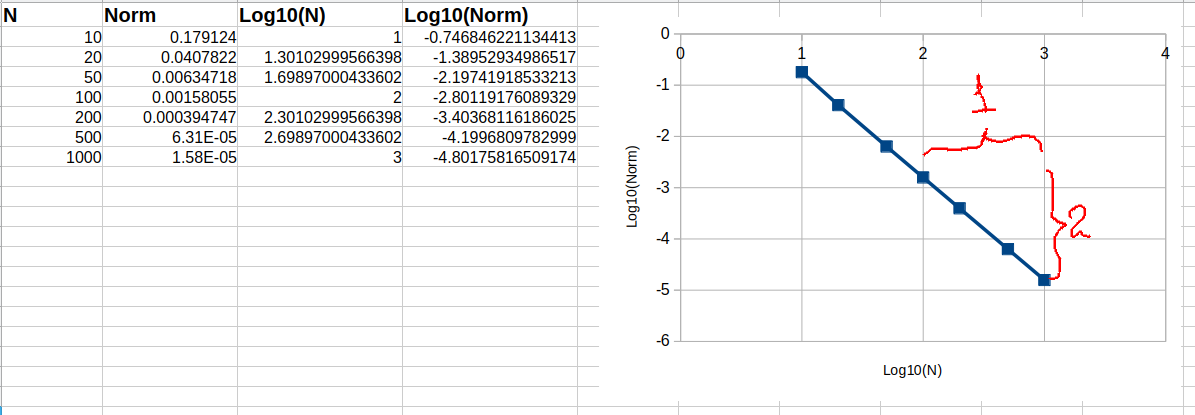
\includegraphics[width=0.9\linewidth]{poisson1_appr.png}
\caption{Сходимость с уменьшением разбиения при решении одномерного уравнения Пуассона}
\label{fig:poisson_convergence}
\end{figure}

Открыв один из cохранённых в процессе работы файлов vtk \ename{poisson1_fdm_n=?.vtk} в paraview
можно посмотреть полученные графики. В файле представлены как точное ``exact'', так и численное решение ``numerical''
(\figref{fig:poisson_graph}).

\begin{figure}[h]
\centering
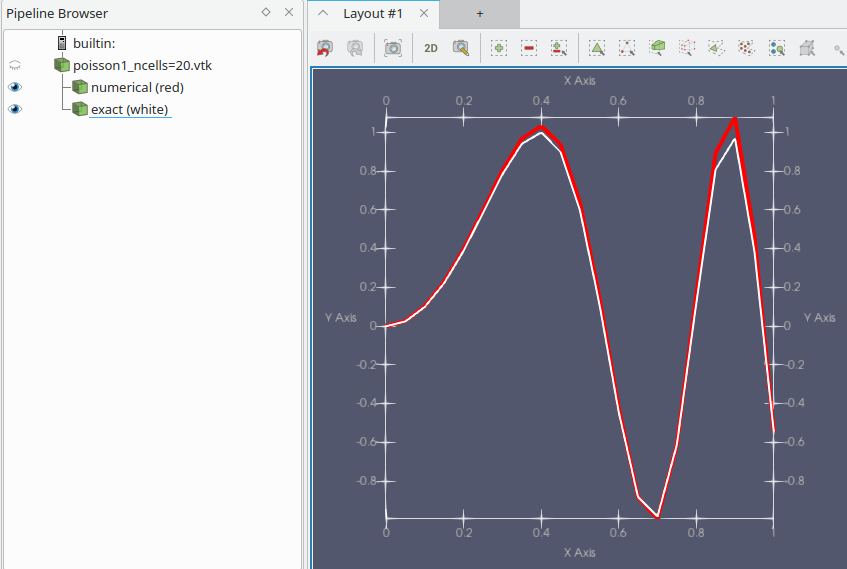
\includegraphics[width=0.9\linewidth]{poisson1_graph.png}
\caption{Сравнение точного и численного решений уравнения Пуассона}
\label{fig:poisson_graph}
\end{figure}


\subsubsection{Детали реализации}
\clisting{open}{"test/poisson_fdm_test.cpp"}
Основная работа по решению задачи проводится в классе \cvar{Problem}.

В его конструкторе происходит инициализация сетки (приватного поля класса) на отрезке $[0, 1]$ с заданным разбиением
\cvar{n_cells}:
\clisting{line}{"Problem"}

В методе \cvar{solve()} производится численное решения задачи и вычисления нормы.
Для этого последовательно
\begin{enumerate}
\item Строится матрица левой части и вектор правой части определяющей системы уравнений.
      Матрицы хранятся в разреженном формате CSR (\secref{sec:csr}), удобном для последовательного чтения.
\item Вызывается решатель СЛАУ. Решение записывается в приватное поле класса \cvar{u}.
\item Вызывается функция вычисления нормы.
\end{enumerate}

\clisting{block}{"double solve()"}

Функции нижнего уровня (используемые в методе \cvar{solve}):
\begin{itemize}
\item
  Сборка левой части СЛАУ. Реализует формулу \eqref{eq:poisson1d_fdm_lhs}.
  Для заполнения матрицы используется формат \cvar{cfd::LodMatrix} (\secref{sec:lodmat}), удобный для непоследовательной записи, который в конце конвертируется CSR.
  \clisting{block}{"approximate_lhs("}
\item
  Сборка правой части СЛАУ. Реализует формулу \eqref{eq:poisson1d_fdm_rhs}.
  \clisting{block}{"approximate_rhs("}
\item
  Вычисление нормы. Реализует формулу \eqref{eq:poisson1d_fdm_norm}.
  \clisting{block}{"compute_norm2"}
\end{itemize}

%\subsection{Разбор программной реализации МКЭ}
\label{sec:fem_programming}
\clisting{open}{"test/poisson_fem_test.cpp"}
Численное решение уравнения Пуассона с граничными
условиями первого рода реализовано в файле
\ename{poisson_fem_test.cpp}.
Будем рассматривать решение одномерной задачи с использованием пирамидальных базисов (тест \ename{[poisson1-fem-lintri]}).
В этом тесте определяется аналитическая функция
$$
f(x) = \sin(10 x^2),
$$
и формулируется уравнение Пуассона с граничными условиями первого рода, для которого эта функция является точным решением.
Далее уравнение Пуассона решается численно и полученный численный результат сравнивается
с точным ответом. Норма полученной ошибки печатается в консоль.

В функции верхнего уровня происходит построение одномерной
сетки, создание рабочего объекта, вызов решения с возвращением нормы полученной ошибки
и вывод данныех (сохранение решения в vtk-файл и печать нормы в консоль):
\clisting{pass}{"[poisson1-fem-linsegm]"}
\clisting{lines-range}{"Grid1D", "std::cout"}
Основная работа происходит в классе \cvar{TestPoissonLinearSegmentWorker}.

\subsubsection{Рабочий объект}
В конструкторе класса \cvar{TestPoissonLinearSegmentWorker}
происходит вызов статической функции \ename{build_fem},
в которой осуществляется сборка массива конечных элементов и таблицы 
связности \quo{элемент--индексы базисов, определённых в элементе} (таблица \cvar{glob} из алгоритма \cvar{eq:fem_vector_assemble}).
Эти данные используются для построения конечноэлементного сборщика (\secref{sec:fem_fem_assembler}).

В родительском класса рабочего объекта 
\cvar{ITestPoisson1FemWorker},
сформулированы аналитические функции, служащие
правой частью, точным решением и условиями первого рода уравнения Пуассона.

А в базовом классе \cvar{ITestPoissonFemWorker} реализованы основные процедуры решения уравнения.
\clisting{to-start}{}
\clisting{block}{"double ITestPoissonFemWorker::solve()"}
Для получения решения сначала собирается левая и правая
часть системы линеных уравнений с учётом граничных условий первого рода,
вызывается решатель системы уравнений и вычислитель нормы ошибки.

В функции сборки левой части СЛАУ сначала происходит поэлементная сборка матрицы, соответствующая алгоритму \cref{eq:fem_matrix_assemble}.
\clisting{to-start}{}
\clisting{block}{"CsrMatrix ITestPoissonFemWorker::approximate_lhs() const"}
При этом вычисление элементной матрицы по формуле \cref{eq:fem_stiff_matrix_xi} осуществляется в абстрактном методе \cvar{element_stiffness_matrix}.
В настоящей реализации используется точное вычисление этого интеграла для одномерного линейного элемента.
в переопределённом методе \cvar{TestPoissonLinearSegmentWorker::element_stiffness_matrix}.

Вставка элементной матрицы в глобальную матрицу осуществляется с
помощью специального сборщика \cvar{fem_} класса \cvar{FemAssembler}.

Далее происходит учёт граничных условий первого рода на матричном уровне, с помощью
постановки единицы на диагональ в строку матрицы, соответсвующую граничному узлу (базису).

По аналогичной процедуре работает и сборка правой части \cvar{approximate_rhs}.

\subsubsection{Конечноэлементный сборщик}
\label{sec:fem_fem_assembler}
Конечноэлементный сборщик \cvar{FemAssembler} -- основной класс, хранящий
всю информацию о текущей конечноэлементной аппроксимации: 
массив конечных элементов и их связность.
Эта информация подаётся ему при конструировании (реализация в файле \ename{cfd/fem/fem_assembler.hpp}).
\clisting{open}{"cfd/fem/fem_assembler.hpp"}
\clisting{lines-range}{"FemAssembler(", ");"}
Связность \cvar{tab_elem_basis} имеет формат \quo{элемент-глобальный базис} и
определяет глобальный индекс для каждого локального базисного индекса.
В рассматренных нами узловых конечных элементах базис связан с узлом сетки.
То есть эта таблица -- это связность локальной и глобальной нумерации узлов сетки для каждой ячейки сетки.

Конечноэлементный сборщик создаётся в методе
\cvar{TestPoissonLinearSegmentWorker::build_fem} итогового
рабочего класса (то есть сборщик специфичен для конкретной сетки
и конкретного выбора типов элементов). Далее он пробрасывается в конструктор базового рабочего класса.

\subsubsection{Концепция конечного элемента}
\clisting{open}{"cfd/fem/fem_element.hpp"}
Класс конечного элемента \cvar{FemElement} определён в файле
\ename{fem/fem_element.hpp} как
\clisting{block}{"struct FemElement"}
Главная задача объекта этого класса -- предоставлять всю информацию для вычисления элементных векторов и матриц,
которые впоследствии используются сборщиком
для создания глобальных матриц.
Для расчёта элементных матриц в свою очередь требуется
\begin{itemize}
\item Геометрия элемента, включающая в себя правило отображения элемента из физической в параметрическую область и матрицу Якоби,
\item Набор shape-функций, заданных в модельной геометрии,
\item Непосредственно правило интегрирования в параметрической области (квадратурные формулы)
\end{itemize}
Каждый из этих трёх алгоритмов определён через объекты классов
\begin{itemize}
\item \cvar{IElementGeometry}
\item \cvar{IElementBasis}
\item \cvar{Quadrature}
\end{itemize}
Полное определение конечного элемента заключается в задании конкретных реализаций первых двух интерфейсов и объекта с квадратурой.

\subsubsubsection{Определение линейного одномерного элемента}
\label{sec:linear_segment_assembly}.
Так, в рассматриваемом нами тесте \ename{"[poisson1-fem-linsegm]"}, используются только линейные одномерные элементы.
Используется следующее определение элемента:
\clisting{open}{"test/poisson_fem_test.cpp"}
\clisting{pass}{"TestPoissonLinearSegmentWorker::build"}
\clisting{lines-range}{"geom =", "FemElement"}
Здесь последовательно определяются:
\begin{itemize}
\item
геометрия отрезка \cvar{geom} -- путём задания двух точек в физичекой плоскости \cvar{p0, p1},
\item
линейный одномерный базис \cvar{basis},
\item
правила интегрирования \cvar{integrals} по параметрическому отрезку $x \in [-1, 1]$
не задаются (используется \cvar{nullptr}), поскольку в дальнейшем
интегрирование ведётся по точным формулам.
\end{itemize}

\subsubsubsection{Геометрические свойства элемента}
\clisting{open}{"cfd/fem/fem_element.hpp"}
Интерфейс \cvar{IElementGeometry}, заданный в файле \ename{cfd/fem/fem_element.hpp},
определяет геометрические свойства элемента:
\clisting{block}{"class IElementGeometry"}
Для вычиселния элементных матриц главным геометрическим свойством
элемента является функция для вычисления матрицы Якоби (\cvar{jacobi}).
В простейших реализациях этого интерфейса для сиплексных геометрий
матрица Якоби постоянна для любой точки, то есть функция \cvar{jacobi} возвращает
один и тот же ответ вне зависимости от переданного аргумента.

Кроме того, этот интерфейс предоставляет функции преобразования координат из физического простравнства
в параметрическое и обратно: \cvar{to_parametric}, \cvar{to_physical}. А также задает центральную точку
в параметрическом пространстве \cvar{parametric_center}.

\subsubsubsection{Элементный базис}
Интерфейс для определения локального элементного базиса (набора shape-функций) имеет вид
\clisting{open}{"cfd/fem/fem_element.hpp"}
\clisting{block}{"class IElementBasis"}
Этот интерфейс работает только с параметрическим пространстсвом
и определяет следующие методы:
\begin{itemize}
\item \cvar{size} -- количество базисных функций;
\item \cvar{parametric_reference_points} -- вектор из параметрических коордианат
      точек, приписанных к соответствующим базисам;
\item \cvar{value} -- значение базисных функций в заданной точке;
\item \cvar{grad} -- градиент (в параметрическом пространстве) базисных функций по заданным точкам.
\item \cvar{upper_hessian} -- верхняя часть матрицы Гессе (вторые производные базисных функций в заданной точке)
\end{itemize}

Конкретная реализация например для линейного треугольного элемента \cvar{TriangleLinearBasis}
(в файле \ename{cfd/fem/elem2d/triangle_linear.cpp})
включает в себя линейный Лагранжев базис в двумерном пространстве согласно
\cref{eq:triangle_linear_basis}:
\clisting{open}{"cfd/fem/elem2d/triangle_linear.cpp"}
\clisting{block}{"TriangleLinearBasis::size"}
\clisting{block}{"TriangleLinearBasis::parametric_reference_points"}
\clisting{block}{"TriangleLinearBasis::value"}
\clisting{block}{"TriangleLinearBasis::grad"}

\subsubsubsection{Квадратурные формулы}
\label{sec:fem_quad_prog}
Объект класса \cvar{Quadrature}, определённого в файле \ename{quadrature.hpp},
предоставляет узловые точки и веса для численного вычисления интегралов.
Гауссовы квадратуры доступны в файлах из папки \ename{cfd/numeric_integration}:
\begin{itemize}
\item \ename{segment_quadrature} -- квадтратуры для интегрирования по отрезку $[-1, 1]$,
\item \ename{triangle_quadrature} -- квадтратуры для интегрирования в треугольнике с узлами $(0, 0)$, $(1, 0)$, $(0, 1)$,
\item \ename{square_quadrature} -- квадтратуры для интегрирования в квадтрате $[-1, 1]\times[-1, 1]$.
\end{itemize}
Последняя цифра в названии конкретной квадтратуры -- степень полинома, для которой она точна.
Например, формула \ename{quadrature_segment_gauss4} -- квадратура для 
интегрирования в отрезке $[-1, 1]$, точная для полинома 4-ой степени.

Для того, чтобы проинтегрировать некоторую заданную координатную функцию $f$
с помощью квадратуры, нужно написать цикл вида
\begin{cppcode}
double f(Point xi){
    ...
}
std::shared_ptr<Quadrature> quad = ...;
double integral = 0.0;
for (size_t k=0; k<quad->size(); ++k){
    Point p = quad->point(k);
    double w = quad->weight(k);
   integral += w*f(p);
}
\end{cppcode}
Либо можно воспользоваться методом \cvar{integrate}:
\begin{cppcode}
double integral = quad->integrate(f);
\end{cppcode}

Для упрощения вычисления специфичных для конечноэлементных
интегралов выражений можно
внутри подинтегральной функции  использовать
вспомогательный класс \cvar{FemElementValue},
позволяющий вычислять значение shape-функций (метод \cvar{phi})
и их производные по физическим координатам (методы \cvar{grad_phi}, \cvar{laplace}, \cvar{divirgence}).

%\subsection{Программа для расчёта течения в каверне по схеме SIMPLE}
\label{sec:prog_cavity_fdm}

\subsubsection{Постановка задачи}

Для иллюстрации работы алгоритма SIMPLE с аппроксимацией методом конечных разностей, представленного в \secref{sec:simple_scheme_fdm}, рассмотрим задачу о 
течении в каверне. Постановку задачи представлена на \figref{fig:cavity}.

\begin{figure}[h]
\centering
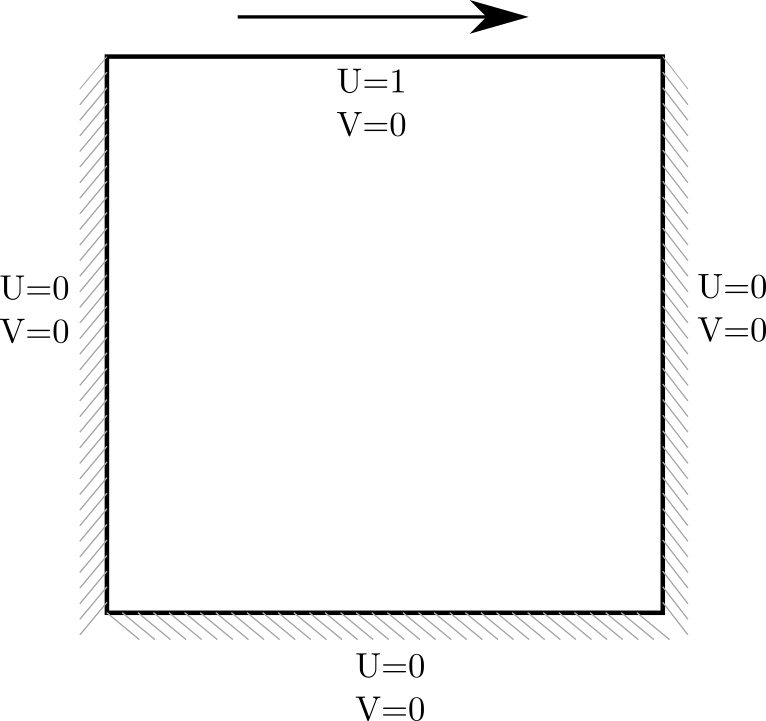
\includegraphics[width=0.4\linewidth]{cavity2d.png}
\caption{Область расчёта задачи о каверне}
\label{fig:cavity}
\end{figure}

Задача реализована в тесте \ename{[cavity-fdm-simple]} в файле \ename{cavity_fdm_test.cpp}.

Программа проводит итерации стартуя от начального нулевого состояния
$u=v=p=0$ до тех пор, пока невязка не достигнет заданного порога.
На каждой итерации поле давления и векторное поле скорости сохраняются
на основной сетке в файл \ename{cavity2.vtk.series}.

Итоговый результат (для $\eps=10^{-2}$) представлен на \figref{fig:cavity-result}.

\begin{figure}[h]
\centering
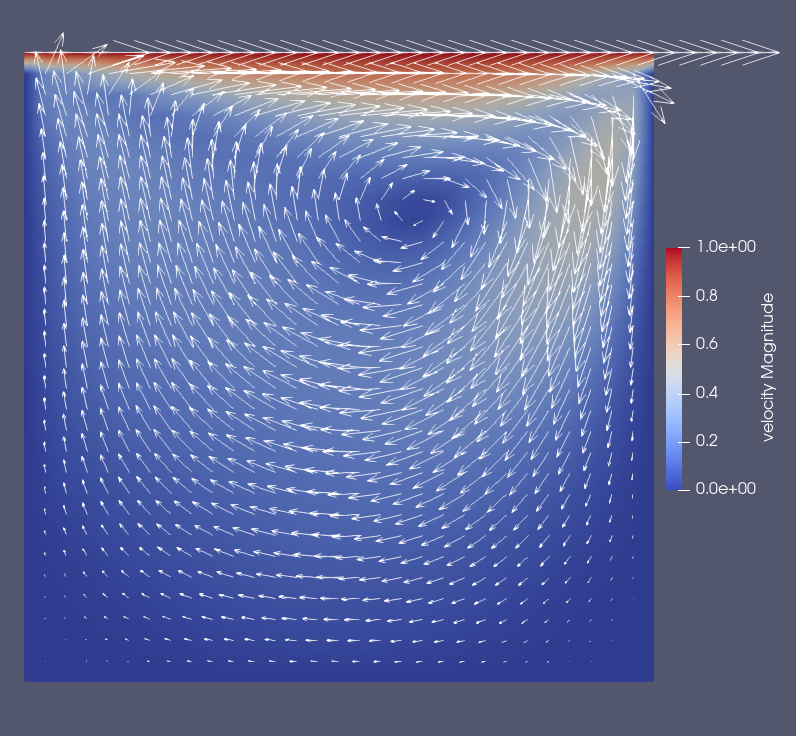
\includegraphics[width=0.7\linewidth]{cavity2d-result.png}
\caption{Область расчёта задачи о каверне}
\label{fig:cavity-result}
\end{figure}

Для отображения вектора поля скорости в Paraview см. справку в \ref{sec:paraview-glyph}.

Для работы с разнесённой сеткой в классе \cvar{cfd::RegularGrid2D}
представлены функции
\begin{itemize}
\item \cvar{cfd::RegularGrid2D::cell_centered_grid()}  -- построить сетку по центрам ячеек (``чёрную'' сетку для $p$),
\item \cvar{cfd::RegularGrid2D::xface_centered_grid()} -- построить сетку по центрам $x$-граней (``синюю'' сетку для $v$),
\item \cvar{cfd::RegularGrid2D::yface_centered_grid()} -- построить сетку по центрам $y$-граней (``красную'' сетку для $u$),
\end{itemize}

и функции перевода индексов
\begin{itemize}
\item \cvar{cfd::RegularGrid2D::cell_centered_grid_index_ip_jp} -- посчитать линейный индекс ``чёрной'' сетки \eqref{eq:ns2d_kipjp},
\item \cvar{cfd::RegularGrid2D::xface_grid_index_ip_j} -- посчитать линейный индекс ``синей'' сетки \eqref{eq:ns2d_kipj},
\item \cvar{cfd::RegularGrid2D::yface_grid_index_i_jp} -- посчитать линейный индекс ``красной'' сетки \eqref{eq:ns2d_kijp}.
\end{itemize}

\subsubsection{Функция верхнего уровня}
\clisting{open}{"test/cavity_fdm_test.cpp"}
\clisting{line}{"[cavity-fdm-simple]"}

Сначала устанавливаются параметры задачи:
число Рейнолдса,
\clisting{line}{"Re"}
параметры алгоритма SIMPLE,
\clisting{lines-range}{"alpha_u", "alpha_p"}
разбиение сетки, 
\clisting{line}{"n_cells"}
максимальное количество итераций 
\clisting{line}{"max_it"}
и значение невязки, при котором итерации прекращаются
\clisting{line}{"double eps"}

Затем происходит инициализация решателя, который
определён в классе \cvar{CavitySimpleWorker}
\clisting{line}{"CavitySimpleWorker"}
и параметров сохранения. Здесь
первым параметром является флаг сохранения
точных сеточных значений, который установлен в \cvar{false},
а также имя файла с итоговым результатом.
Таким образом сохраняться будет только решение,
интерполированное на основную сетку.
Для целей отладки программы (для просмотра действительных, не интерполированных полей решения)
следует первый флаг установить в \cvar{true}. Тогда помимо \ename{cavity2.vtk.series}, будут
создаваться также файлы \ename{cavity2-u}, \ename{cavity2-v}, \ename{cavity2-p}.
\clisting{until}{"_saver"}

Потом происходит установка начальных значений искомых сеточных векторов: $u=v=p=0$
\clisting{lines-range}{"u_init", "set_uvp"}

и начинается итерационный процесс.
\clisting{line}{"for"}

Внутри цикла
выполняется шаг итерационного процесса, который
возвращает значение итоговой невязки в переменную \cvar{nrm}.
\clisting{line}{"step"}

На печать выводится индекс итерации, значение невязки и значение давления в правом верхнем узле (для контроля сходимости)
\clisting{line}{"cout"}

Сохраняется состояние решателся на пройденную итерацию
\clisting{line}{"save_current"}

и производится проверка на сходимость
\clisting{block}{"if (nrm < eps)"}

В конце производится проверка: при установленных параметрых решение
должно сойтись за 9 итераций:
\clisting{line}{"CHECK"}

\subsubsection{Поля класса решателя}
\clisting{to-start}{}
Класс \cvar{CavitySimpleWorker} хранит в себе набор полей,
характеризующих состояние итерационного процесса.
Некоторые из этих полей (параметры решателя) постоянны (\cvar{const}) и
определяются непосредственно перед вызовом конструктора в инициализаторе. Другие
меняются с продвижением по итерациям.

Среди постоянных полей заданы 4 сетки: основная \cvar{_grid},
``чёрная'' сетка \cvar{_cc_grid} (cell-centered) для давления,
``красная'' сетка \cvar{_yf_grid} (y-face) для $u$,
``синяя'' сетка \cvar{_xf_grid} (x-face) для $v$ (\figref{fig:staggered_grid}).
\clisting{pass}{"private"}
\clisting{until}{"yf_grid_"}
Далее заданы скалярные параметры: число Рейнольдса, шаги сетки и параметры алгоритма SIMPLE
\clisting{until}{"alpha_p_"}

Далее следуют сеточные вектора, характеризующие текущее состояние решателя:
найденные на последней итерации давление и скорости.
\clisting{until}{"v_;"}

Также определяется данные для
сборки систем уравнений: внедиагональные и диагональные коэффициенты диффузии для \cref{eq:ns2d_au,eq:ns2d_ava}
и значения $d^u=d^u$, требуемые для сборки \eqref{eq:ns2d_pprime_slae}.
Поскольку используется постоянные шаги по времени эти коэффициенты являются скалярами.
Ниже задан инициализированный решатель системы уравнений для $p'$.
\clisting{until}{"p_prime_solver_"}

Хранятся левая и правая части систем уравнений \eqref{eq:ns2d_ustar_slae}, \eqref{eq:ns2d_vstar_slae}
для определения пробных значений скорости и расчета невязки.
\clisting{until}{"rhs_v_;"}

Указатели на классы, помогающие сохранять найденные вектора в vtk - формат.
Эти классы инициализируются только в случае, если пользователь указал на 
необходимость сохранения.
\clisting{until}{"writer_all_;"}

\subsubsection{Инициализация решателя}
\clisting{to-start}{}

В секции инициализации конструктора
созаются сетки в единичном квадрате и переписываются параметры решения.
Далее в теле конструктора вычисляются значения
$d^u=d^v$ по формулам \cref{eq:ns2d_du_fdm,eq:ns2d_dv_fdm}
и собирается решатель для $p'$. Как было указано ранее,
матрица системы $A^p$ не меняется
с продвижением по итерациям, поэтому этот решатель можно собрать один раз
до начала счёта.

\clisting{block}{"CavitySimpleWorker::CavitySimpleWorker"}

Начальные значения устанавливаются через вызов функции \cvar{set_uvp}.
Эти начальные значения будут использоваться в качестве значений
с предыдущего итерационного слоя на первой итерации.

В функции происходит переписывание переданных векторов
в приватные поля класса.
\clisting{lines-range}{"set_uvp", "p_"}

После этого данных в классе-решателе достаточно,
для сборки матриц $A^u, A^v$ и правых частей
$b^u, b^v$ для системы уравнений \eqref{eq:ns2d_ustar_slae}, \eqref{eq:ns2d_vstar_slae}.
\clisting{until}{"v_slae()"}

Если посмотреть на выражение для невязки \eqref{eq:ns2d_residual} убрав в нём крышки над переменными, то можно
убедится, что оно аппроксимируется в виде
\begin{equation*}
    r_u = A^u u - b^u.
\end{equation*}
Поэтому после сборки систем уравнений движения, можно вычислить невязку, характеризующую
отклонение установленного в этой процедуре решения от желаемого:
\clisting{until-close}{}

\subsubsection{Шаг итерации SIMPLE}
\clisting{to-start}{}
Осуществляется в процедуре
\clisting{block}{"double CavitySimpleWorker::step()"}
и представляет собой буквальное пошаговое следование алгоритму SIMPLE (\ref{sec:simple-algo}).
В конце опять вызывается функция \cvar{set_uvp} для сборки матриц для следующей итерации
и подсчёта невязки на текущей итерации.

\subsubsection{Сборка системы уравнений для поправки давления}
\clisting{to-start}{}

Сборка системы уравнений \eqref{eq:ns2d_pprime_slae}
осуществляется в процедуре
\clisting{line}{"void CavitySimpleWorker::assemble_p_prime_solver()"}
Сборка происходит с использованием матрицы формата \cvar{cfd::LodMatrix},
удобного для непоследовательной записи.
\clisting{until}{"LodMatrix"}
Заполнение происходит в цикле по раздвоенным индексам $ij$
``чёрной'' сетки для давления:
\clisting{until}{"size_t i"}
Внутри цикла устанавливаются флаги, характеризующие граничный статус текущего узла
\clisting{until}{"is_top"}
Вычисляется значение сквозного индекса по формуле \eqref{eq:ns2d_kipjp}
\clisting{until}{"ind0"}
и значения коэффициентов в формулах \eqref{eq:ns2d_ap}. Поскольку
сетка равномерная, эти значения не меняются для разных узлов
\clisting{until}{"coef_y"}
Далее формулы \eqref{eq:ns2d_ap}
применяются для заполнения матриц
с учётом аппроксимированного граничного условия \eqref{eq:ns2d_bc3}.
Так, запись
\clisting{until-close}{}
для всех неправых узлов с линейным индексом \cvar{ind0} вычисляет индекс 
узла, расположенного правее него с линейным индексом \cvar{ind1},
добавляет слагаемое в диагональный (первое из уравнений \eqref{eq:ns2d_ap}) и
вычитает из недиагонального (четвёртое из уравнений \eqref{eq:ns2d_ap}) элемента
строки \cvar{ind0}.
Для правых узлов работает граничное условие \eqref{eq:ns2d_ap} и выполнять эту процедуру
не нужно.

После заполнения в матрицу вводится граничное условие \eqref{eq:ns2d_bc4}
\clisting{line}{"set_unit_row"}

И матрица передаётся в решатель СЛАУ предварительно сконверованная в формат \cvar{cfd::CsrMatrix}
\clisting{until}{"set_matrix"}

Правая часть собирается заново на каждой итерации по формуле \eqref{eq:ns2d_bp}.
Её реализация представлена в функции
\clisting{line}{"CavitySimpleWorker::compute_p_prime"}
Сначала собирается правая часть системы \eqref{eq:ns2d_pprime_slae} по формуле \eqref{eq:ns2d_bp}:
\clisting{block}{"for (size_t i"}
потом осуществляется установка граничного условия \eqref{eq:ns2d_bc4}
\clisting{line}{"rhs[0]"}
и вызывается решатель СЛАУ
\clisting{until-close}{}

\subsubsection{Сборка системы уравнений для пробной скорости}
\clisting{to-start}{}

Сборка системы \eqref{eq:ns2d_ustar_slae} (как правой, так и левой частей) реализована
в функции
\clisting{line}{"CavitySimpleWorker::assemble_u_slae"}

Основной цикл идёт по негрничным узлам ``красной'' сетки,
в котором реализуются формулы \eqref{eq:ns2d_au}
\clisting{pass}{"internal"}
\clisting{block}{"for (size_t", "rhs"}

Как было отмечено в пункте \ref{sec:simple-bc},
граничные условия первого рода в этом уравнении
учитываются двумя разными способами:
узлы расположенные непосредственно на границе (нижней и верхней)
учитываются по схеме \eqref{eq:ns2d_bc1}, которая реализована в цикле
\clisting{to-start}{}
\clisting{block}{"for (size_t j = 0; j < grid_.ny(); ++j)"}

А фиктивные узлы, возникающие при обработке
узлов расположенных в полушаге от границ (левой и правой),
обрабатываются по схеме \eqref{eq:ns2d_bc2}.
Эта схема реализована в виде
препроцессинга алгоритма добавления элемента в матрицу в лямбда-функции
\clisting{to-start}{}
\clisting{pass}{"assemble_u_slae"}
\clisting{block}{"add_to_mat"}

Эта лямбда вызывается везде, где нужно добавить в строку \cvar{row_index}
и колонку, соответствующую узлу \cvar{ij_col}, значение \cvar{value}.
Она перехватывает ситуации с ``фиктивным'' узлом ($j=-1, j=n_y$)
и применяет алгоритм \eqref{eq:ns2d_bc2}.


\section{Формулы и обозначения}
\subsection{Векторы}

\subsubsection{Обозначение}

Геометрические вектора обозначаются жирным шрифтом $\vec v$.
Скалярные координаты вектора -- через нижний индекс с обозначением
оси координат: $\left(v_x, v_y, v_z\right)$.
Если вектор $\vec u$ -- вектор скорости, то его декартовые координаты
имеют специальное обозначение $\vec u = \left(u, v, w\right)$.
Единичные вектора, соответствующие осям координат, обозначаются 
знаком $\hat\cdot$: $\vec{\hat x}$, $\vec{\hat y}$, $\vec{\hat z}$.
Координатные векторы обозначаются по символу первой оси. Например, $\vec x = (x, y, z)$ или $\vec \xi = (\xi, \eta, \zeta)$.

Операции в векторами имеют следующее обозначение (расписывая в декартовых координатах):
\begin{itemize}
\item
Умножение на скалярную функцию
\begin{equation}
\label{eq:vec_scalar}
f \vec u = (f u_x)\vec{\hat x} + (f u_y)\vec{\hat y} + (f u_z)\vec{\hat z};
\end{equation}
\item
Скалярное произведение
\begin{equation}
\label{eq:vec_dot}
\vec u \cdot \vec v = u_x v_x + u_y v_y + u_z v_z;
\end{equation}
\item
Векторное произведение
\begin{equation}
\label{eq:vec_cross}
\vec u\times\vec v = 
\left|
\begin{array}{ccc}
\vec{\hat x} & \vec{\hat y} & \vec{\hat z} \\
u_x & u_y & u_z \\
v_x & v_y & v_z
\end{array}
\right| = 
\left(u_y v_z - u_z v_y\right)\vec{\hat x} -
\left(u_x v_z - u_z v_x\right)\vec{\hat y} +
\left(u_x v_y - u_y v_x\right)\vec{\hat z}.
\end{equation}

\end{itemize}

В двумерном случае можно считать, что $u_z = v_z = 0$.
Тогда результатом векторного произведения согласно \cref{eq:vec_cross} 
будет вектор, направленный перпендикулярно плоскости $xy$:
$$
\vec u \times \vec v = (u_x v_y - u_y v_x)\vec{\hat z}.
$$
При работе с двумерными задачами, где ось $\vec z$ отсутствует,
обычно результатом векторного произведения считают скаляр
\begin{equation}
\label{eq:vec_cross_2d}
2D: \; \vec u \times \vec v = u_x v_y - u_y v_x.
\end{equation}
Геометрический смысл этого скаляра: площадь
параллелограмма, построенного на векторах $\vec u$ и $\vec v$.


\subsubsection{Набла--нотация}

Символ $\nabla$ -- есть псевдовектор, который выражает
покоординатные производные.
Для декартовой системы координат $(x, y, z)$ он запишется в виде
$$
\nabla = \left( \dfr{}{x}, \; \dfr{}{y}, \; \dfr{}{z} \right).
$$
В радиальной $(r, \phi, z)$:
$$
\nabla = \left( \dfr{}{r}, \; \frac{1}{r}\dfr{}{\phi}, \; \dfr{}{z} \right).
$$
В цилиндрической $(r, \theta, \phi)$:
$$
\nabla = \left( \dfr{}{r}, \; \frac{1}{r}\dfr{}{\theta}, \; \frac{1}{r\sin\theta}\dfr{}{\phi} \right).
$$
Удобство записи дифференциальных выражений с использованием $\nabla$ заключается в независимости записи от
вида системы координат.
Но если требуется обозначить производную по конкретной координате,
то, по аналогии с обычными векторами, это делается через нижний индекс:
$$
\nabla_n f = \dfr{f}{n}.
$$

Для этого символа справедливы все векторные операции, описанные ранее.
Так, применение $\nabla$ к скалярной функции аналогично умножению вектора
на скаляр \cref{eq:vec_scalar} (здесь и далее приводятся покоординатные выражения для декартовой системы):
\begin{equation}
\label{eq:del_grad}
\nabla f  = \left(\nabla_x f, \; \nabla_y f, \; \nabla_z f\right) = \dfr{f}{x}\vec{\hat x} + \dfr{f}{y}\vec{\hat y} + \dfr{f}{z}\vec{\hat z}.
\end{equation}
Результатом этой операции является вектор.

Скалярное умножение $\nabla$ на вектор $\vec v$ по аналогии с \cref{eq:vec_dot} -- есть дивергенция:
\begin{equation}
\label{eq:del_div}
\nabla \cdot \vec v  = \dfr{v_x}{x} + \dfr{v_y}{y} + \dfr{v_z}{z}
\end{equation}
результат которой -- скалярная функция.

Двойное применение $\nabla$ к скалярной функции -- это оператор Лапласа:
\begin{equation}
\label{eq:del_laplace}
\nabla \cdot \nabla f  = \nabla^2 f = \dfrq{f}{x} + \dfrq{f}{y} + \dfrq{f}{z}
\end{equation}

Ротор -- аналог векторного умножнения \cref{eq:vec_cross}:
\begin{equation}
\label{eq:del_rotor}
\nabla\times\vec v = 
\left|
\begin{array}{ccc}
\vec{\hat x} & \vec{\hat y} & \vec{\hat z} \\
\nabla_x & \nabla_y & \nabla_z \\
v_x & v_y & v_z
\end{array}
\right| = 
\left(\dfr{v_z}{y} - \dfr{v_y}{z}\right)\vec{\hat x} -
\left(\dfr{v_z}{x} - \dfr{v_x}{z}\right)\vec{\hat y} +
\left(\dfr{v_y}{x} - \dfr{v_x}{y}\right)\vec{\hat z}.
\end{equation}

\subsection{Интегрирование}
\label{sec:partint} 

\subsubsection{Формула Гаусса--Остроградского}

Формула Гаусса--Остроградского, связывающая
интегрирование по объёму $E$ с интегрированием по границе этого объёма $\Gamma$,
для векторного поля $\vec v$ имеет вид
\begin{equation}
\label{eq:partint_div}
\arint{\nabla\cdot\vec v}{E}{\vec x} = \arint{v_n}{\Gamma}{s},
\end{equation}
где $\vec n$ -- внешняя по отношению к области $E$ нормаль.
Смысл этой формулы можно проиллюстрировать на одномерном примере.
Пусть одномерное векторное поле $v_x = f(x)$ на отрезке $E = [a, b]$ задано
функцией, представленной на \figref{fig:div1d}.
\begin{figure}[h!]
\centering
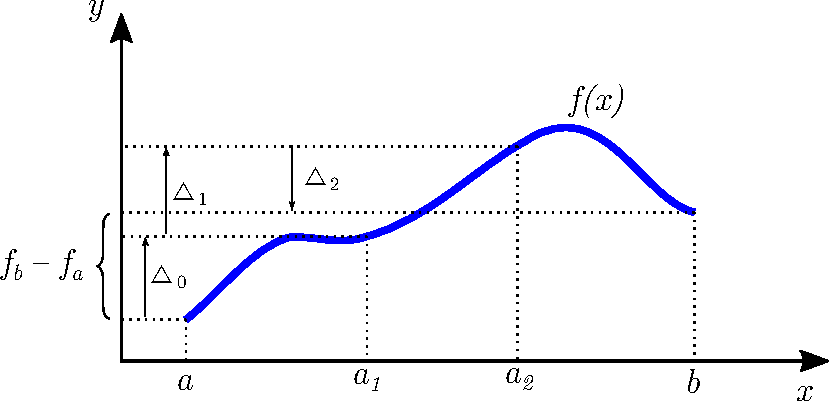
\includegraphics[width=0.6\linewidth]{div1d.pdf}
\caption{Формула Гаусса-Остроградского в одномерном случае}
\label{fig:div1d}
\end{figure}
Разобъем область на $N=3$ равномерных подобласти длины $h$. Тогда
расписывая интеграл как сумму, а производную через конечную разность, получим
$$
\arint{\dfr{f}{x}}{E}{x} \approx \sum_{i=0}^{2} h \left(\dfr{f}{x}\right)_{i+\tfrac12}
\approx\sum_{i=0}^{2}(f_{i+1} - f_{i})
= \triangle_0 + \triangle_1 + \triangle_2 = f_b - f_a.
$$
Очевидно что, при устремлении $N\to\infty$ правая часть предыдущего выражения не изменится.
То есть, сумма всех изменений функции в области есть изменение функции по её границам:
$$
\int\limits_{a}^{b}\dfr{f}{x}\,dx = f(b) - f(a).
$$
А формула \cref{eq:partint_div} -- есть многомерное обобщение этого выражения.

Если в формулу \cref{eq:partint_div}
подставить выражение
$\vec v = \sum_i u \vec e_i$,
где $\vec e_i$ -- единичный базисный вектор в направлении $x_i$,
то получим
\begin{equation*}
\arint{\sum_i\dfr{u}{x_i} \vec e_i}{E}{\vec x} = \arint{u \, \sum_i \vec e_i \cdot \vec n}{\Gamma}{s}.
\end{equation*}
Перепишем в набла нотации:
\begin{equation}
\label{eq:partint_grad}
\arint{\nabla u}{E}{\vec x} = \arint{u \, \vec n}{\Gamma}{s}.
\end{equation}


\subsubsection{Интегрирование по частям}

Подставив в \cref{eq:partint_div} $\vec v = f\vec u$, где $f$ -- некоторая скалярная функция, и 
расписав дивергенцию в виде
$$\nabla\cdot(f\vec u) = f\nabla\vec u + \vec u \cdot \nabla f$$
получим формулу интегрирования по частям
\begin{equation}
\label{eq:partint}
\arint{\vec u \cdot \nabla f}{E}{\vec x} = \arint{f u_n}{\Gamma}{s} - \arint{f\nabla\cdot \vec u}{E}{\vec x}
\end{equation}
Распишем некоторые частные случаи для формулы \cref{eq:partint}.
Для $\vec u = (n_x, 0, 0)$ получим
\begin{equation}
\label{eq:partint_ugrad_}
\arint{\dfr{f}{x}}{E}{\vec x} = \arint{f \cos(\vecangle{n}{x})}{\Gamma}{s}
\end{equation}
При $\vec u = \nabla g$
\begin{equation}
\label{eq:partint_laplace_fg}
\arint{f \nabla^2 g }{E}{\vec x} = \arint{f\dfr{g}{n}}{\Gamma}{s} - \arint{\nabla f \cdot \nabla g}{E}{\vec x}
\end{equation}
При $f=1$ и $\vec u = \nabla g$
\begin{equation}
\label{eq:partint_laplace}
\arint{\nabla^2 g}{E}{\vec x} = \arint{\dfr{g}{n}}{\Gamma}{s}
\end{equation}

\subsubsection{Численное интегрирование в заданной области}
Квадратурная формула
\begin{equation}
\label{eq:quadrature_formula}
\arint{f(\vec x)}{E}{\vec x} = \sum_{i=0}^{N-1} w_i f(\vec x_i)
\end{equation}
Она определяется заданием узлов интегрирования $\vec x_i$ 
и соответствующих весов $w_i$.

\subsection{Интерполяционные полиномы}

\subsubsection{Многочлен Лагранжа}

\subsubsubsection{Узловые базисные функции}

Рассмотрим функцию $f(\xi)$, заданную в области $D$.
Внутри этой области зададим $N$ узловых
точек $\xi_i, i=\overline{0,N-1}$.
Приближение функции $f$ будем искать в виде
\begin{equation}
\label{eq:nodal_basis}
f(\xi) \approx \sum_{i=0}^{N-1} f_i \phi_i(\xi),
\end{equation}
где  $f_i = f(\xi_i)$, $\phi_i$ -- узловая базисная функция.
Потребуем, чтобы это выражение выполнялось точно для всех
заданных узлов интерполяции $\xi = \xi_i$. Тогда, исходя из определения \cref{eq:nodal_basis}, запишем условие 
на узловую базисную функцию
\begin{equation}
\label{eq:nodal_bases_conditions}
\phi_i(\xi_j) = 
\begin{cases}
1, &\quad i = j, \\
0, &\quad i \neq j.
\end{cases}
\end{equation}
Дополнительно потребуем, чтобы формула \cref{eq:nodal_basis} была
точной для постоянных функций
$$
f(\xi)=\const \hence f_i = \const.
$$
Тогда для любого $\xi$ должно выполняться условие
\begin{equation}
\label{eq:nodal_bases_unitsum}
\sum_{i=0}^{N-1} \phi_i(\xi) = 1, \qquad \xi \in D.
\end{equation}

Задача построения интерполяционной функции состоит
в конкретном определении узловых базисов
$\phi_i(\xi)$ по заданному набору
узловых точек $\xi_i$ и значениям
функции в них $f_i$. Будем искать базисы
в виде многочленов вида
\begin{equation}
\label{eq:nodal_basis_1d_decomp}
\phi_i(\xi) = \sum_{a} A_i^{(a)} \xi^{a} =
A_i^{(0)} + 
A_i^{(1)} \xi + 
A_i^{(2)} \xi^2 +  \ldots, \qquad i = \overline{0, N-1}.
\end{equation}
Определять коэффициенты $A^{(a)}_i$ будем из условий \cref{eq:nodal_bases_conditions},
которое даёт $N$ линейных уравнений относительно неизвестных $A_i^{(a)}$ для каждого $i=\overline{0, N-1}$.
Таким образом, в выражениях \cref{eq:nodal_basis_1d_decomp} должно быть
ровно $N$ слагаемых.
Будем использовать последовательный набор степеней: $a=\overline{0,N-1}$.
Выпишем систему линейных уравнений для $0$-ой базисной функции
\begin{equation*}
\begin{aligned}
& \phi_0(\xi_0) = A_0^{(0)} + A_0^{(1)} \xi_0 + A_0^{(2)} \xi_0^2 + A_0^{(3)} \xi_0^3 + \ldots = 1, \\
& \phi_0(\xi_1) = A_0^{(0)} + A_0^{(1)} \xi_1 + A_0^{(2)} \xi_1^2 + A_0^{(3)} \xi_1^3 + \ldots = 0, \\
& \phi_0(\xi_2) = A_0^{(0)} + A_0^{(1)} \xi_2 + A_0^{(2)} \xi_2^2 + A_0^{(3)} \xi_2^3 + \ldots = 0, \\
& \ldots
\end{aligned}
\end{equation*}
или в матричном виде
\begin{equation*}
\left(
\begin{array}{ccccc}
1 & \xi_0 & \xi_0^2 & \xi_0^3 & \ldots \\[5pt]
1 & \xi_1 & \xi_1^2 & \xi_1^3 & \ldots \\[5pt]
1 & \xi_2 & \xi_2^2 & \xi_2^3 & \ldots \\[5pt]
1 & \xi_3 & \xi_3^2 & \xi_3^3 & \ldots \\[5pt]
\ldots &&&&
\end{array}
\right)
\left(
\begin{array}{c}
A_0^{(0)} \\[5pt]
A_0^{(1)} \\[5pt]
A_0^{(2)} \\[5pt]
A_0^{(3)} \\[5pt]
\vdots
\end{array}
\right)
=
\left(
\begin{array}{c}
1 \\[5pt]
0 \\[5pt]
0 \\[5pt]
0 \\[5pt]
\vdots
\end{array}
\right)
\end{equation*}
Записывая аналогичные выражения для остальных базисных функций, получим систему матричных уравнений
вида $C A = E$:
\begin{equation*}
\left(
\begin{array}{ccccc}
1 & \xi_0 & \xi_0^2 & \xi_0^3 & \ldots \\[5pt]
1 & \xi_1 & \xi_1^2 & \xi_1^3 & \ldots \\[5pt]
1 & \xi_2 & \xi_2^2 & \xi_2^3 & \ldots \\[5pt]
1 & \xi_3 & \xi_3^2 & \xi_3^3 & \ldots \\[5pt]
\ldots &&&&
\end{array}
\right)
\left(
\begin{array}{ccccc}
A_0^{(0)} & A_1^{(0)} & A_2^{(0)} & A_3^{(0)} & \ldots\\[5pt]
A_0^{(1)} & A_1^{(1)} & A_2^{(1)} & A_3^{(1)} &       \\[5pt]
A_0^{(2)} & A_1^{(2)} & A_2^{(2)} & A_3^{(2)} &       \\[5pt]
A_0^{(3)} & A_1^{(3)} & A_2^{(3)} & A_3^{(3)} &       \\[5pt]
\vdots
\end{array}
\right)
=
\left(
\begin{array}{ccccc}
1 & 0 & 0 & 0 & \ldots \\[5pt]
0 & 1 & 0 & 0 &        \\[5pt]
0 & 0 & 1 & 0 &        \\[5pt]
0 & 0 & 0 & 1 &        \\[5pt]
\vdots
\end{array}
\right)
\end{equation*}
Отсюда матрица неизвестных коэффициентов $A$ определится как
\begin{equation}
\label{eq:nodal_basic_amat}
A = C^{-1} = 
\left(
\begin{array}{ccccc}
1 & \xi_0 & \xi_0^2 & \xi_0^3 & \ldots \\[5pt]
1 & \xi_1 & \xi_1^2 & \xi_1^3 & \ldots \\[5pt]
1 & \xi_2 & \xi_2^2 & \xi_2^3 & \ldots \\[5pt]
1 & \xi_3 & \xi_3^2 & \xi_3^3 & \ldots \\[5pt]
\ldots &&&&
\end{array}
\right) ^{-1}.
\end{equation}

Подставляя полином \cref{eq:nodal_basis_1d_decomp} в условие согласованности \cref{eq:nodal_bases_unitsum},
получим требование
\begin{equation*}
\sum_{i=0}^{N-1} A_i^{(a)} = 
\begin{cases}
1, \quad a=0, \\
0, \quad a=\overline{1,N-1}.
\end{cases}
\end{equation*} 
То есть сумма всех свободных членов в интерполяционных полиномах должна
быть равна единице, а сумма коэффициентов при остальных степенях -- нулю.
Можно показать, что это свойство выполняется для любой матрицы $A=C^{-1}$,
в случае, если первый столбец матрицы $C$ состоит из единиц.
То есть условие согласованности требует наличие свободного члена
с интерполяционном полиноме.


\subsubsubsection{Интерполяция в параметрическом отрезке}
\label{sec:segment_bases}
Будем рассматривать область интерполяции $D=[-1, 1]$.
В качестве первых двух узлов интерполяции возьмем границы области:
$\xi_0 = -1$, $\xi_1 = 1$.
\paragraph{Линейный базис}
Будем искать интерполяционный базис в виде
$$
\phi_i(\xi) = A_i^{(0)} + A_i^{(1)} \xi.
$$
на основе двух условий:
$$
\phi_i(-1) = A_i^{(0)} - A_i^{(1)} = \delta_{0i}, \quad \phi_i(1) = A_i^{(0)} + A_i^{(1)}\delta_{1i}.
$$
Составим матрицу $C$, записав эти условия в матричном виде
$$
C =
\left(
\begin{array}{l|rr}
      & A^{(0)} & A^{(1)}\\
\hline
\phi(-1) & 1 & -1 \\[5pt]
\phi(1) & 1 &  1 \\[5pt]
\end{array}
\right)
$$
и, согласно \cref{eq:nodal_basic_amat}, найдём матрицу коэффициентов
$$
A =
\left(
\begin{array}{cc}
A_0^{(0)} & A_1^{(0)} \\[5pt]
A_0^{(1)} & A_1^{(1)} \\[5pt]
\end{array}
\right) = C^{-1} =
\left(
\begin{array}{l|rr}
     & \phi_0   & \phi_1  \\
\hline
1    & \frac12  & \frac12 \\[5pt]
\xi  & -\frac12 & \frac12 \\[5pt]
\end{array}
\right).
$$
Отсюда узловые базисные функции примут вид (\figref{fig:basis1d_linear})
\begin{equation}
\label{eq:segment_linear_basis}
\begin{aligned}
&\phi_0(\xi) = \frac{1 - \xi}{2}, \\
&\phi_1(\xi) = \frac{1 + \xi}{2}.
\end{aligned}
\end{equation}
Окончательно интерполяционная функция из определения \cref{eq:nodal_basis}
примет вид
$$
f(\xi) \approx \frac{1 - \xi}{2} f(-1) + \frac{1 + \xi}{2} f(1).
$$
\begin{figure}[h!]
\centering
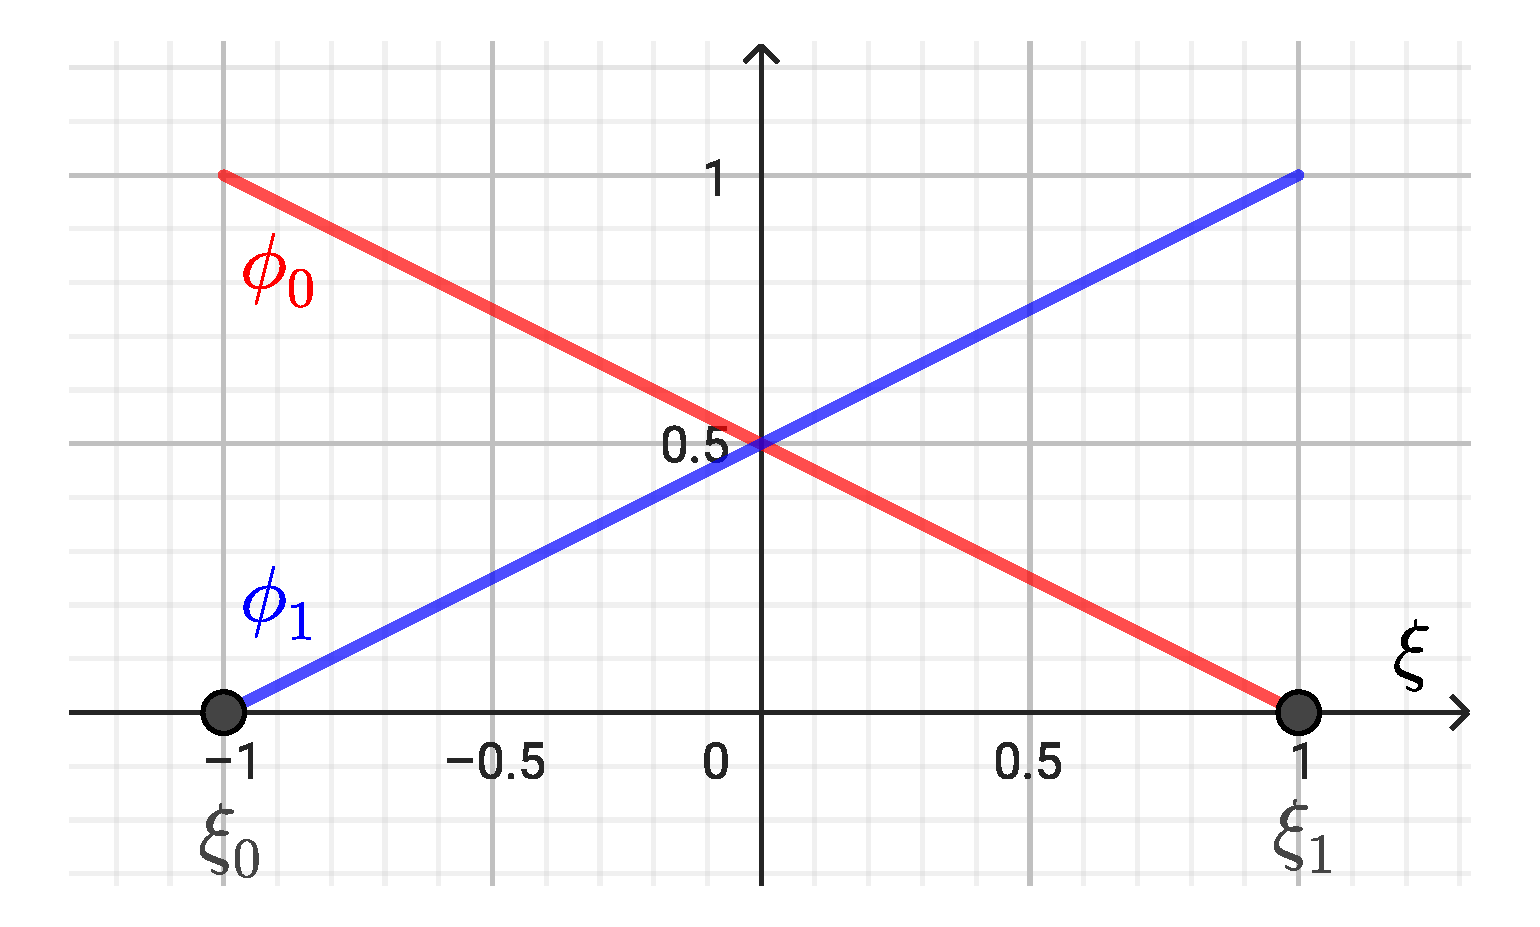
\includegraphics[width=0.4\linewidth]{basis1d_linear.pdf}
\caption{Линейный базис в параметрическом отрезке}
\label{fig:basis1d_linear}
\end{figure}

\paragraph{Квадратичный базис}
Будем искать интерполяционный базис в виде
$$
\phi_i(\xi) = A_i^{(0)} + A_i^{(1)} \xi + A_i^{(2)} \xi^2.
$$
По сравнению с линейным случаем, в форму базиса добавился ещё один неизвестый коэффициент $A_i^{(2)}$,
поэтому в набор условий \cref{eq:nodal_bases_conditions} требуется ещё одно уравнение (ещё одна узловая точка).
Поместим её в центр параметрического сегмента $\xi_2 = 0$. Далее будем действовать по
аналогии с линейным случаем:
$$
C = \left(
\begin{array}{l|rrr}
         &  A^{(0)} & A^{(1)}   & A^{(2)} \\ 
\hline
\phi(-1) & 1 & -1 & 1\\[5pt]
\phi(1)  & 1 &  1 & 1\\[5pt]
\phi(0)  & 1 &  0 & 0
\end{array}
\right)
\hence
A = C^{-1} = \left(
\begin{array}{l|rrr}
       & \phi_0   & \phi_1   & \phi_2 \\
\hline
 1     & 0        &  0       &  1     \\[5pt]
 \xi   & -\frac12 &  \frac12 &  0     \\[5pt]
 \xi^2 &  \frac12 &  \frac12 & -1     \\[5pt]
\end{array}
\right).
$$
Узловые базисные функции для квадратичной интерполяции примут вид (\figref{fig:basis1d_quadratic})
\begin{equation}
\label{eq:segment_quadratic_basis}
\begin{aligned}
&\phi_0(\xi) = \frac{\xi^2 - \xi}{2}, \\
&\phi_1(\xi) = \frac{\xi^2 + \xi}{2}, \\
&\phi_2(\xi) = 1 - \xi^2.
\end{aligned}
\end{equation}

\begin{figure}[h!]
\centering
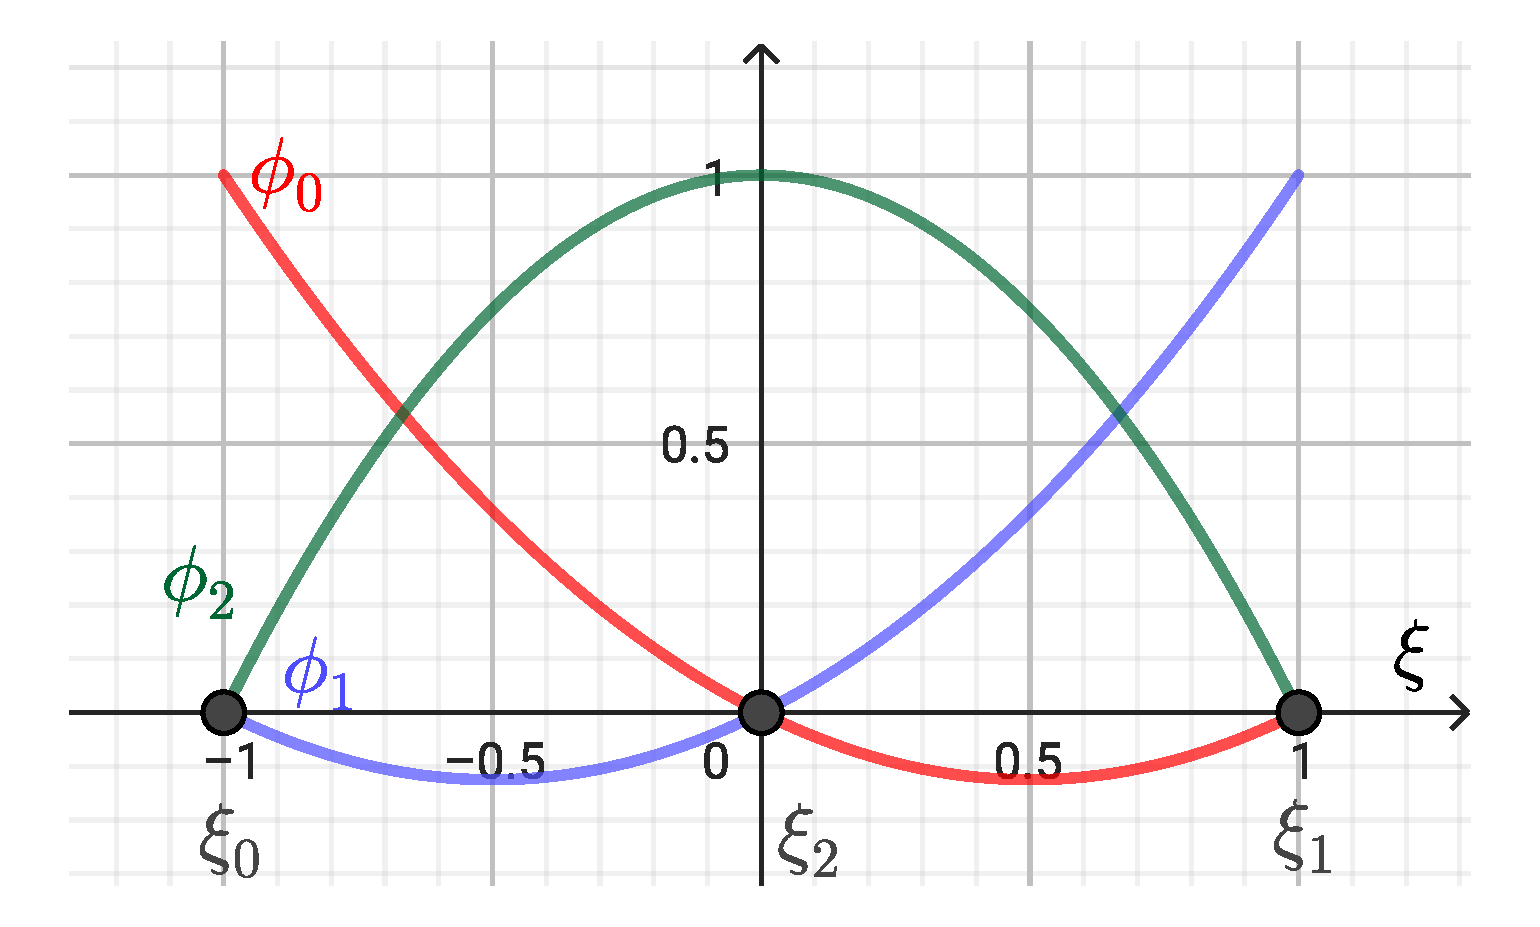
\includegraphics[width=0.4\linewidth]{basis1d_quadratic.pdf}
\caption{Квадратичный базис в параметрическом отрезке}
\label{fig:basis1d_quadratic}
\end{figure}

\paragraph{Кубический базис}
Интерполяционный базис будет иметь вид
$$
\phi_i(\xi) = A_i^{(0)} + A_i^{(1)} \xi + A_i^{(2)} \xi^2 + A_i^{(3)} \xi^3.
$$
Для нахождения четырёх коэффициентов нам понадобится четыре узла интерполяции.
Две из них -- это границы параметрического отрезка. Остальные две разместим
так, чтобы разбить отрезок на равные интервалы:
$\xi_2 = -\tfrac13$, $\xi_3 = \tfrac13$.
Далее вычислим матрицу коэффициентов:
$$
C =
\left(
\begin{array}{l|rrrr}
                &  A^{(0)}  &  A^{(1)}      & A^{(2)}     & A^{(3)}         \\
\hline
\phi(-1)        &  1  & -1        & 1         &  -1           \\[5pt]
\phi( 1)        &  1  & 1         & 1         &   1           \\[5pt]
\phi(-\tfrac13) &  1  & -\tfrac13 & \tfrac19  &  -\tfrac1{27} \\[5pt]
\phi(\tfrac13)  &  1  &  \tfrac13 & \tfrac19  &   \tfrac1{27}
\end{array}
\right)
\hence
A = C^{-1} =
\frac{1}{16}
\left(
\begin{array}{l|rrrr}
      & \phi_0 & \phi_1 & \phi_2 & \phi_3 \\
\hline
1     & -1     & -1     &   9    &  9     \\[5pt]
\xi   &  1     & -1     & -27    &  27    \\[5pt]
\xi^2 &  9     &  9     & -9     & -9     \\[5pt]
\xi^3 & -9     &  9     &  27    & -27   
\end{array}
\right)
$$
Узловые базисные функции для квадратичной интерполяции примут вид (\figref{fig:basis1d_cubic})
\begin{equation}
\label{eq:segment_cubic_basis}
\begin{aligned}
&\phi_0(\xi) = \frac{1}{16}\left(-1 + \xi + 9 \xi^2 -9 \xi^3\right), \\
&\phi_1(\xi) = \frac{1}{16}\left(-1 - \xi + 9 \xi^2 +9 \xi^3\right), \\
&\phi_2(\xi) = \frac{1}{16}\left(9 -27 \xi - 9\xi^2 + 27 \xi^3\right), \\
&\phi_3(\xi) = \frac{1}{16}\left(9 +27 \xi - 9\xi^2 - 27 \xi^3\right), \\
\end{aligned}
\end{equation}

\begin{figure}[h!]
\centering
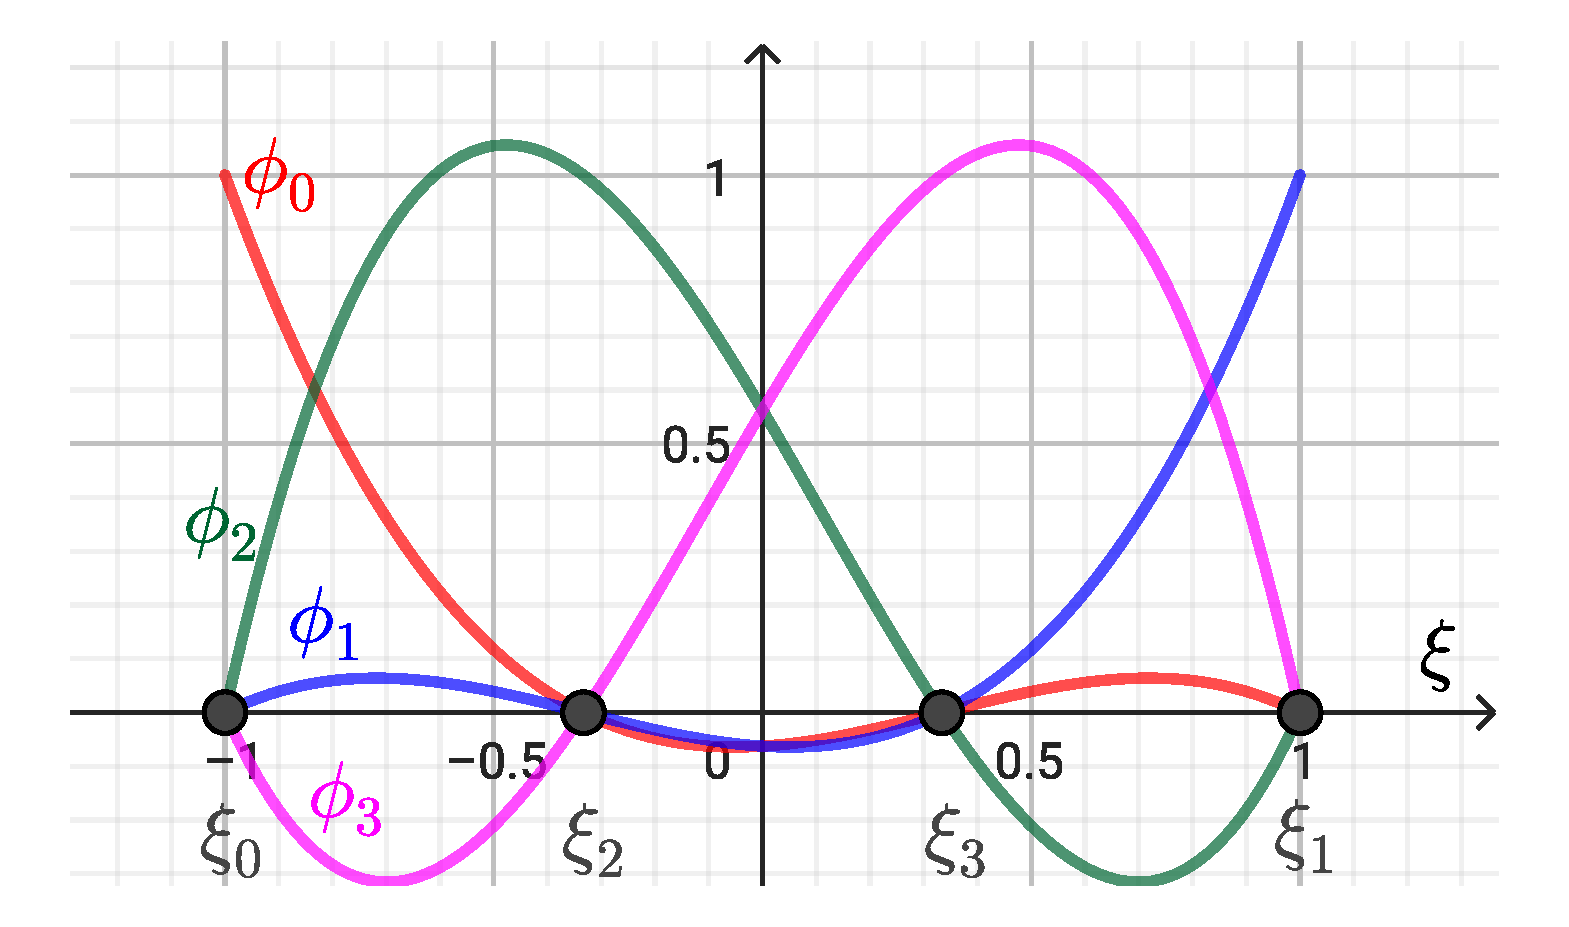
\includegraphics[width=0.4\linewidth]{basis1d_cubic.pdf}
\caption{Кубический базис в параметрическом отрезке}
\label{fig:basis1d_cubic}
\end{figure}

На \figref{fig:basis1d_compare} представлено сравнение результатов
аппроксимации функции $f(x) = -x + \sin(2 x + 1)$ линейным, квадратичным и кубическим базисом.
Видно, что все интерполяционные приближения точно попадают в функцию в своих
узлах интерполяции, а между узлами происходит аппроксимация полиномом соответствующей степени.

\begin{figure}[h!]
\centering
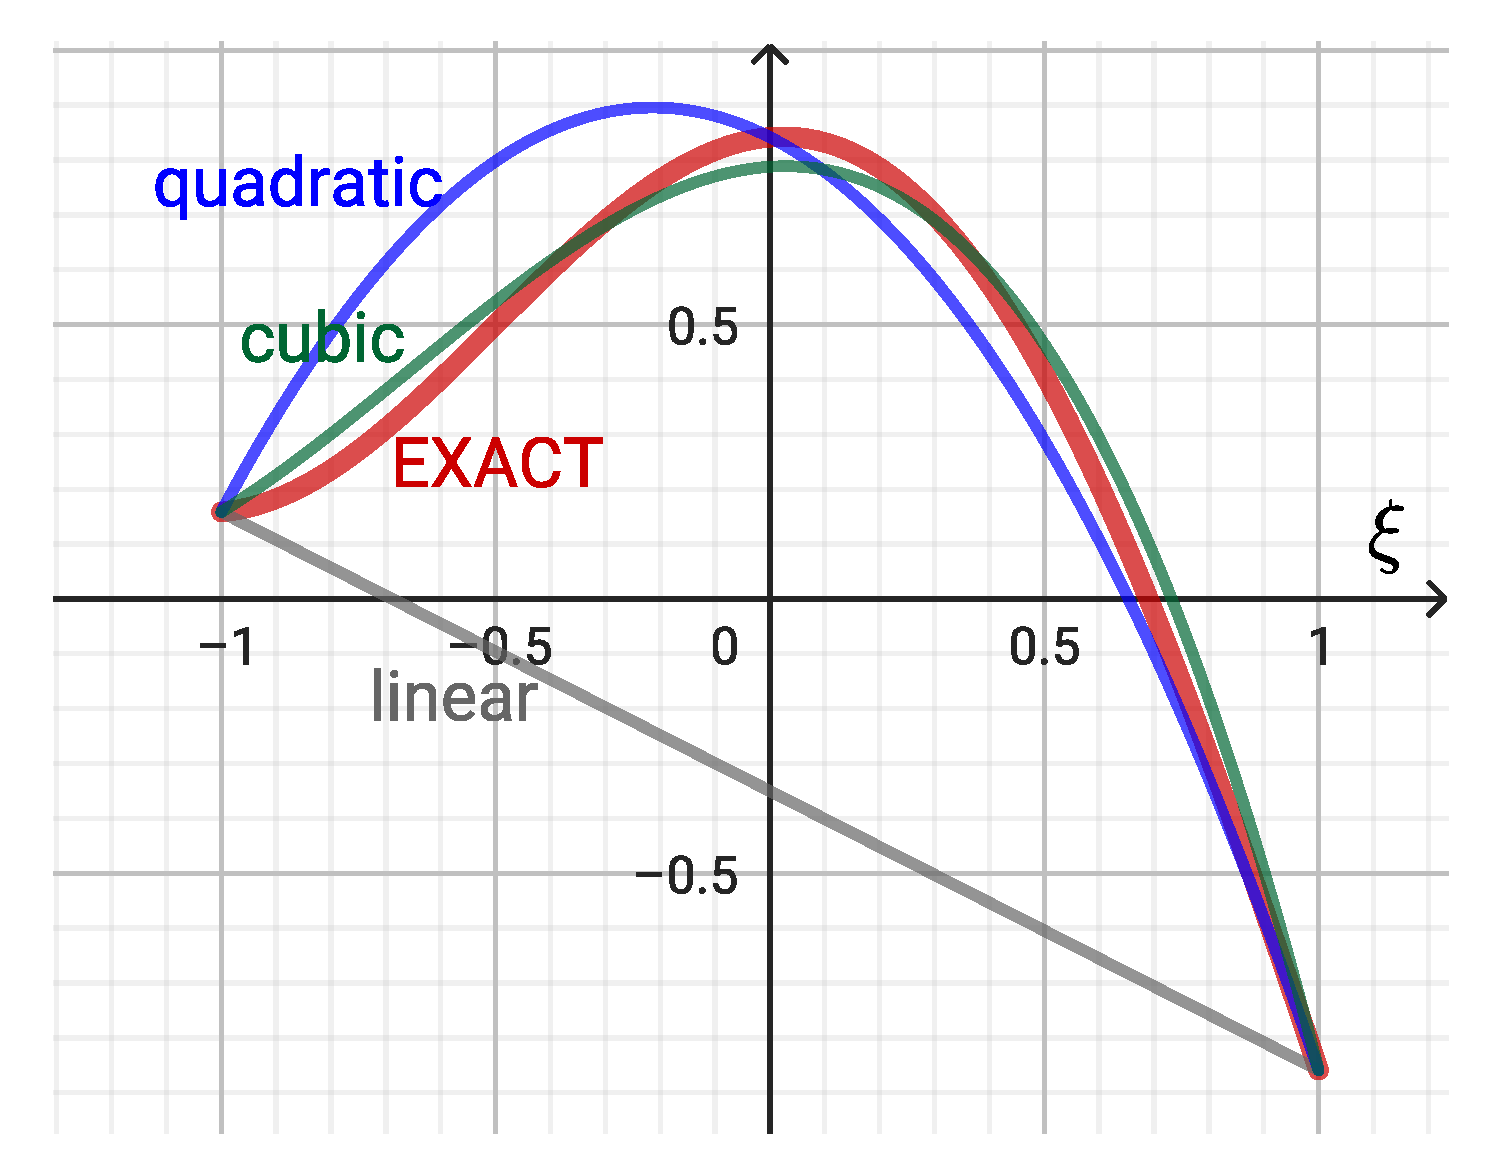
\includegraphics[width=0.4\linewidth]{basis1d_compare.pdf}
\caption{Результат интерполяции}
\label{fig:basis1d_compare}
\end{figure}

\subsubsubsection{Интерполяция в параметрическом треугольнике}
\label{sec:triangle_bases}
Теперь рассмотрим двумерное обобщение формулы
\begin{figure}[h!]
\centering
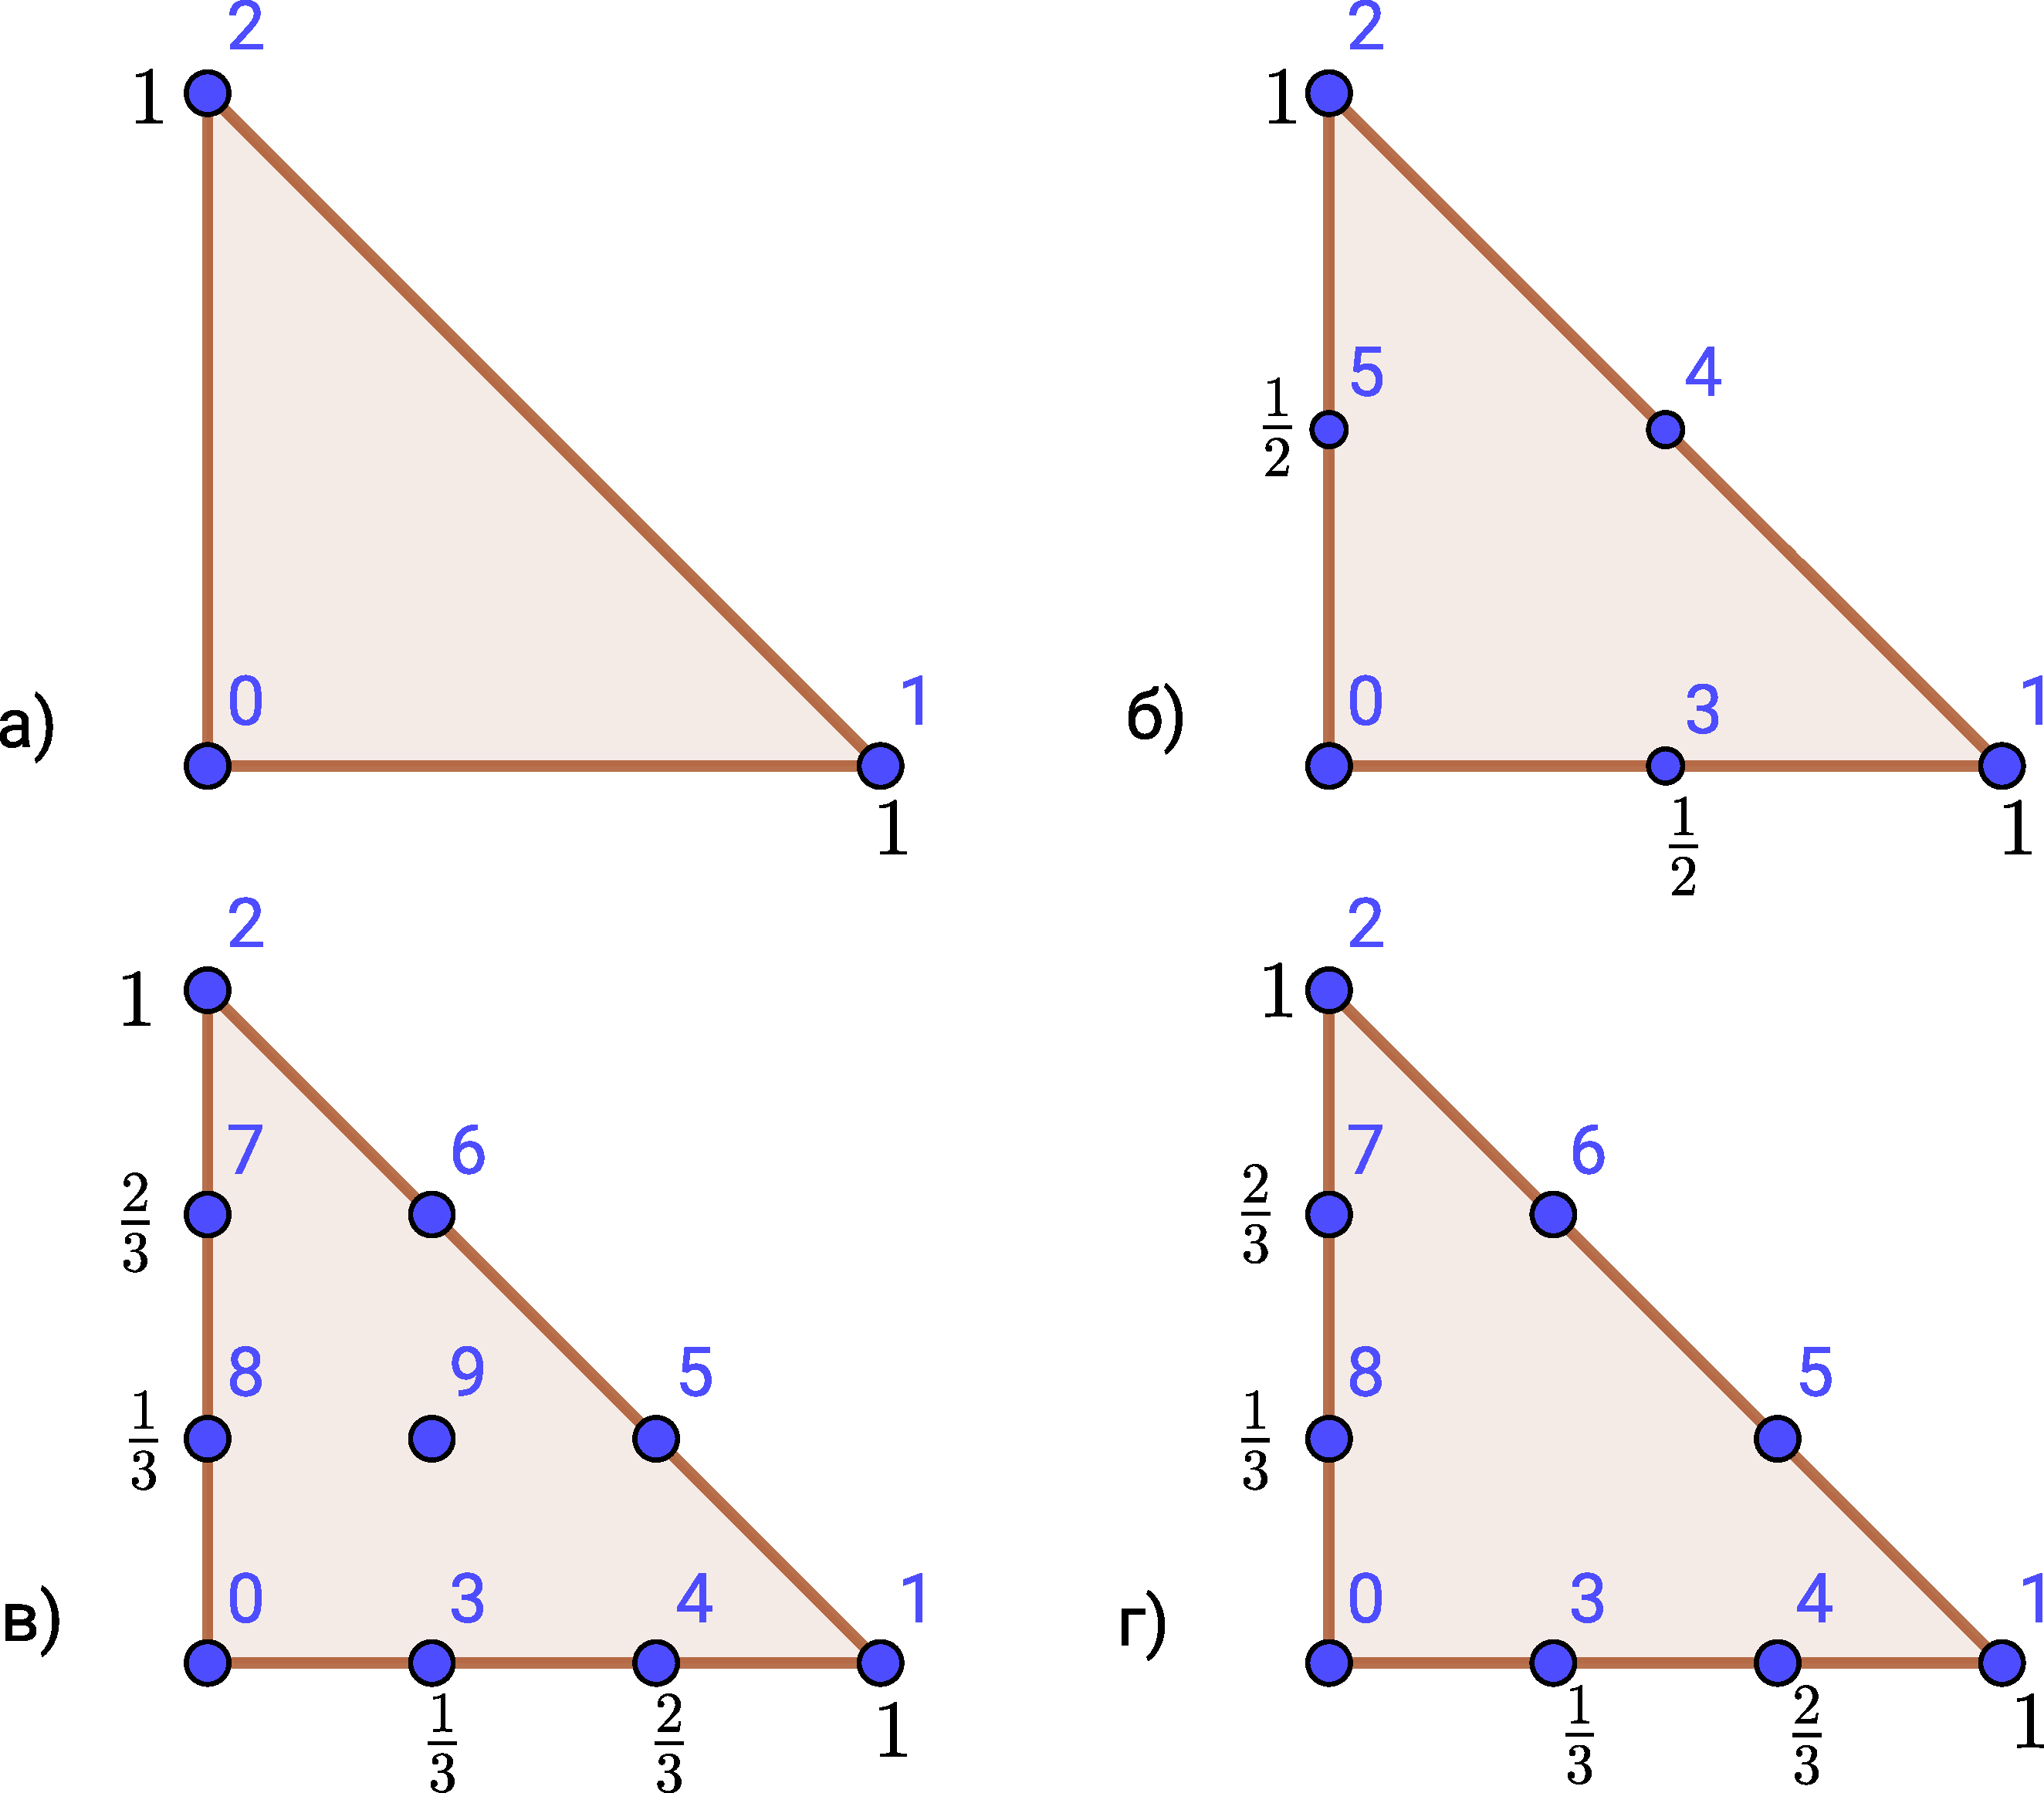
\includegraphics[width=0.5\linewidth]{triangle_basis_points.pdf}
\caption{Расположение узловых точек в параметрическом треугольнике. а) линейный базис, б) квадратичный базис, в) кубический базис, г) неполный кубический базис}
\label{fig:triangle_basis_points}
\end{figure}
\paragraph{Линейный базис}

\begin{equation*}
\phi_i(\xi, \eta) = A_i^{(00)} + A_i^{(10)} \xi + A_i^{(01)} \eta.
\end{equation*}
\begin{equation*}
C = \left(
\begin{array}{l|ccc}
                  & A^{(00)}   & A^{(10)} & A^{(01)} \\
\hline
\phi(0, 0) & 1   & 0   & 0    \\[5pt]
\phi(1, 0) & 1   & 1   & 0    \\[5pt]
\phi(0, 1) & 1   & 0   & 1
\end{array}
\right)
\hence
A = C^{-1} = 
\left(
\begin{array}{l|rrr}
     & \phi_0 & \phi_1 & \phi_2 \\
\hline
1    & 1      & 0      & 0      \\[5pt]
\xi  &-1      & 1      & 0      \\[5pt]
\eta &-1      & 0      & 1
\end{array}
\right)
\end{equation*}

\begin{equation}
\label{eq:triangle_linear_basis}
\begin{aligned}
&\phi_0(\xi, \eta) = 1 - \xi - \eta, \\
&\phi_1(\xi, \eta) = \xi, \\
&\phi_2(\xi, \eta) = \eta, \\
\end{aligned}
\end{equation}

\begin{figure}[h!]
\centering
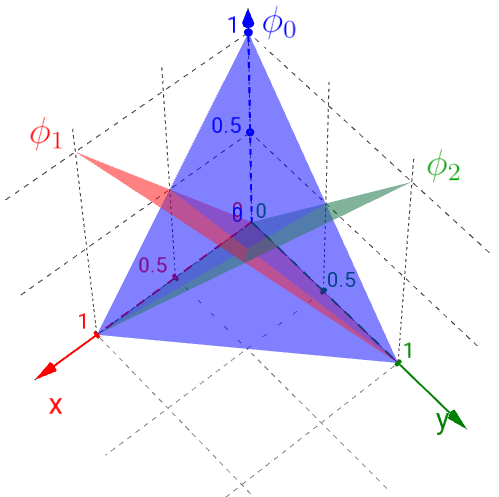
\includegraphics[width=0.4\linewidth]{basis2d_linear.png}
\caption{Линейный базис в параметрическом треугольнике}
\label{fig:basis2d_linear}
\end{figure}


\paragraph{Квадратичный базис}
\begin{equation*}
\phi_i(\xi, \eta) = A_i^{(00)} + A_i^{(10)} \xi + A_i^{(01)} \eta + A_i^{(11)} \xi \eta + A_i^{(20)} \xi^2 + A_i^{(02)} \eta^2.
\end{equation*}

\begin{equation*}
C =
\left(
\begin{array}{l|cccccc}
                     & A^{(00)} & A^{(10)}      & A^{(01)}  & A^{(11)}  & A^{(20)}    & A^{(02)}   \\[5pt]
\hline
\phi(0, 0)               & 1 &  0       &  0          &   0      &    0     &   0      \\[5pt]
\phi(1, 0)               & 1 &  1       &  0          &   0      &    1     &   0      \\[5pt]
\phi(0, 1)               & 1 &  0       &  1          &   0      &    0     &   1      \\[5pt]
\phi(\tfrac12, 0)        & 1 & \tfrac12 &  0          &   0      & \tfrac14 &   0      \\[5pt]
\phi(\tfrac12, \tfrac12) & 1 & \tfrac12 &  \tfrac12   & \tfrac14 & \tfrac14 & \tfrac14 \\[5pt]
\phi(0, \tfrac12)        & 1 &  0       &  \tfrac12   &   0      &    0     & \tfrac14 
\end{array}
\right)
\hence
A = \left(
\begin{array}{l|rrrrrr}
        & \phi_0 & \phi_1 & \phi_2 & \phi_3 & \phi_4 & \phi_5 \\[5pt]
\hline
1       & 1  &  0 & 0 & 0 & 0 & 0\\[5pt]
\xi     & -3 & -1 & 0 & 4 & 0 & 0\\[5pt]
\eta    & -3 & 0 & -1 & 0 & 0 & 4\\[5pt]
\xi\eta & 4 & 0 & 0 & -4 & 4 & -4\\[5pt]
\xi^2   & 2 & 2 & 0 & -4 & 0 & 0 \\[5pt]
\eta^2  & 2 & 0 & 2 & 0 & 0 & -4
\end{array}
\right)
\end{equation*}

\begin{figure}[h!]
\centering
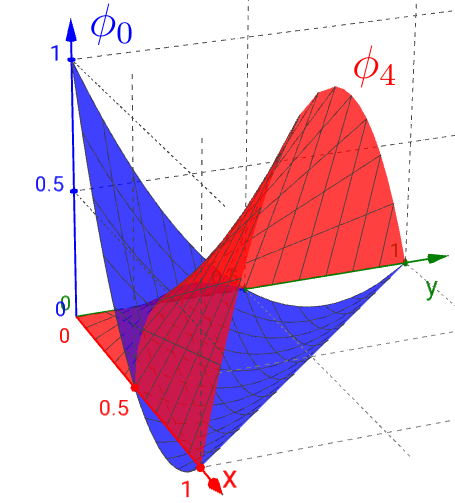
\includegraphics[width=0.3\linewidth]{basis2d_quadratic.png}
\caption{Квадратичные функции $\phi_0$, $\phi_4$ в параметрическом треугольнике}
\label{fig:basis2d_quadratic}
\end{figure}

\paragraph{Кубический базис}
TODO

\paragraph{Неполный кубический базис}
TODO

\subsubsubsection{Интерполяция в параметрическом квадрате}
\begin{figure}[h!]
\centering
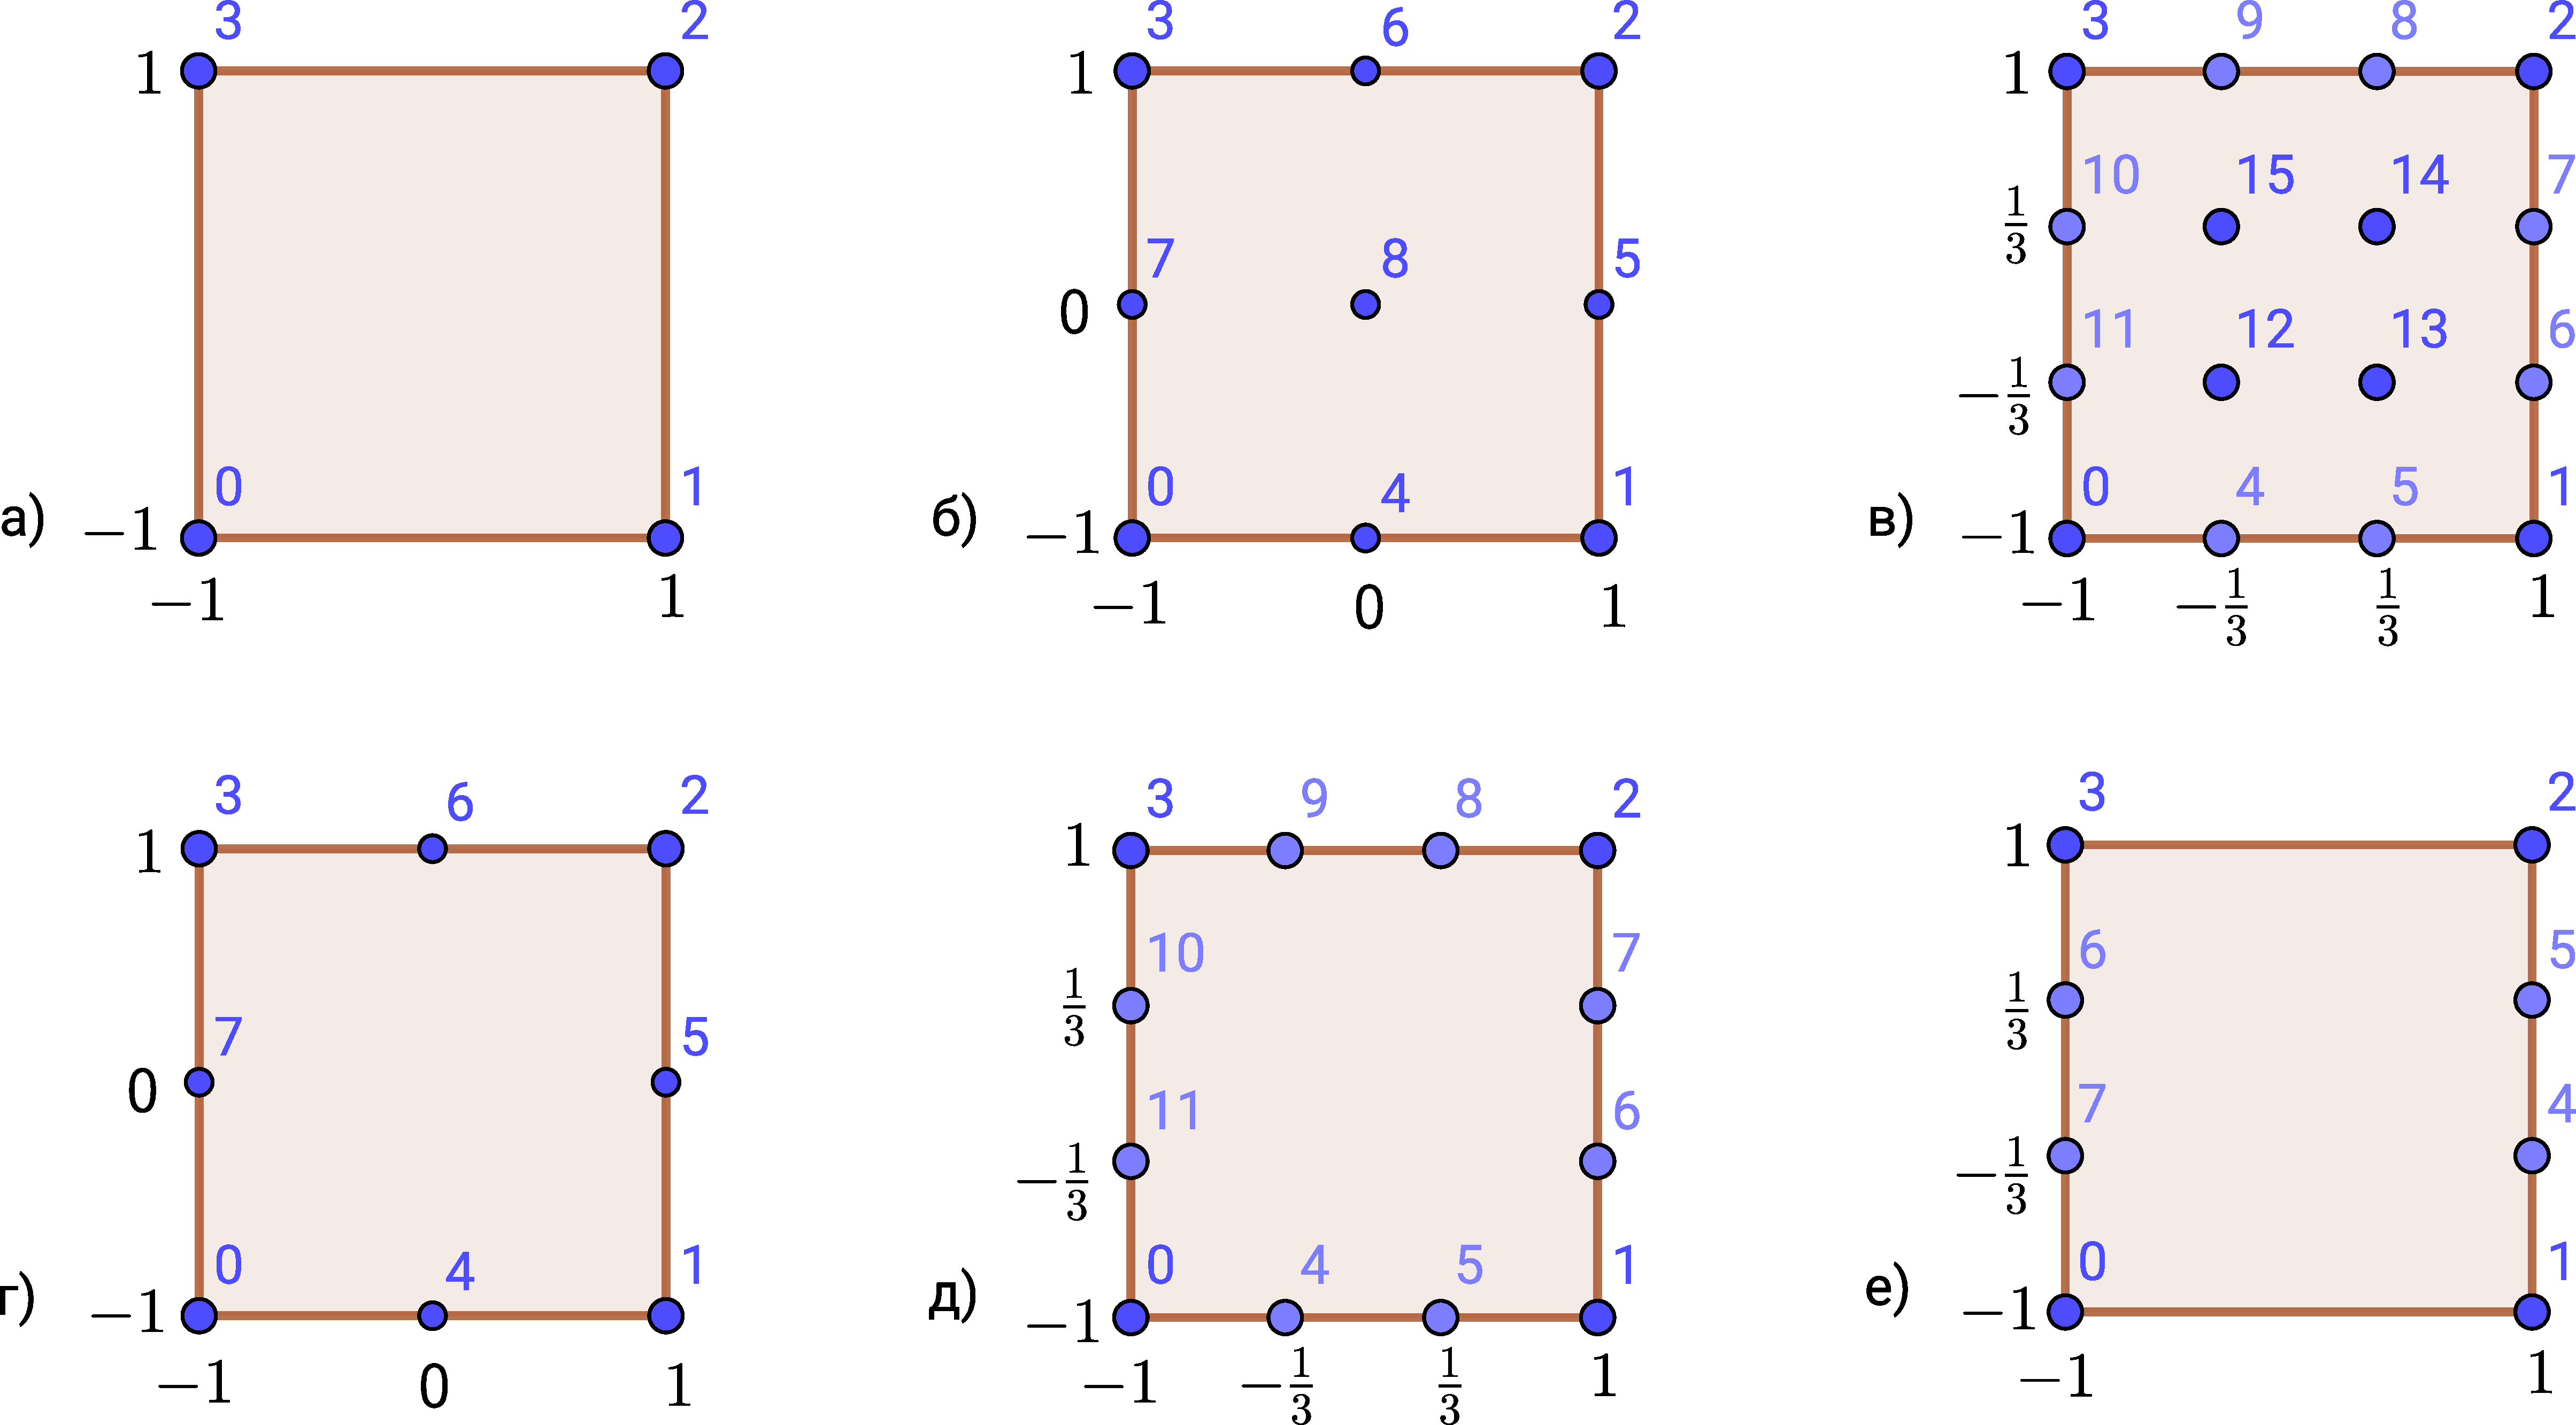
\includegraphics[width=0.7\linewidth]{quadrangle_basis_points.pdf}
\caption{Расположение узловых точек в параметрическом квадрате}
\label{fig:quadrangle_basis_points}
\end{figure}

\paragraph{Билинейный базис}
\begin{equation*}
\phi_i = A^{00}_i + A^{10}_i \xi + A^{01}_i \eta + A^{11}_i \xi\eta.
\end{equation*}

\begin{equation*}
C = \left(
\begin{array}{l|rrrr}
                      & A^{(00)} & A^{(10)} & A^{(01)} & A^{(11)} \\
\hline
\phi(-1, -1) & 1 & -1  & -1   &  1      \\[5pt] 
\phi( 1, -1) & 1 &  1  & -1   & -1      \\[5pt]
\phi( 1,  1) & 1 &  1  &  1   &  1      \\[5pt]
\phi(-1,  1) & 1 & -1  &  1   & -1      \\[5pt]
\end{array}
\right)
\hence
A = C^{-1} = \frac14\left(
\begin{array}{l|rrrr}
        & \phi_0 & \phi_1 & \phi_2 & \phi_3\\
\hline
1       & 1 & 1 & 1 & 1\\[5pt]
\xi     & -1 & 1 & 1 & -1\\[5pt]
\eta    & -1 & -1 & 1 & 1\\[5pt]
\xi\eta & 1 & -1 & 1 & -1
\end{array}
\right)
\end{equation*}

\begin{equation}
\label{eq:quadrangle_bilinear_basis}
\begin{aligned}
&\phi_0(\xi, \eta) = \frac{1-\xi-\eta+\xi\eta}{4}\\[10pt]
&\phi_1(\xi, \eta) = \frac{1+\xi-\eta-\xi\eta}{4}\\[10pt]
&\phi_2(\xi, \eta) = \frac{1+\xi+\eta+\xi\eta}{4}\\[10pt]
&\phi_3(\xi, \eta) = \frac{1-\xi+\eta-\xi\eta}{4}
\end{aligned}
\end{equation}

\begin{figure}[h!]
\centering
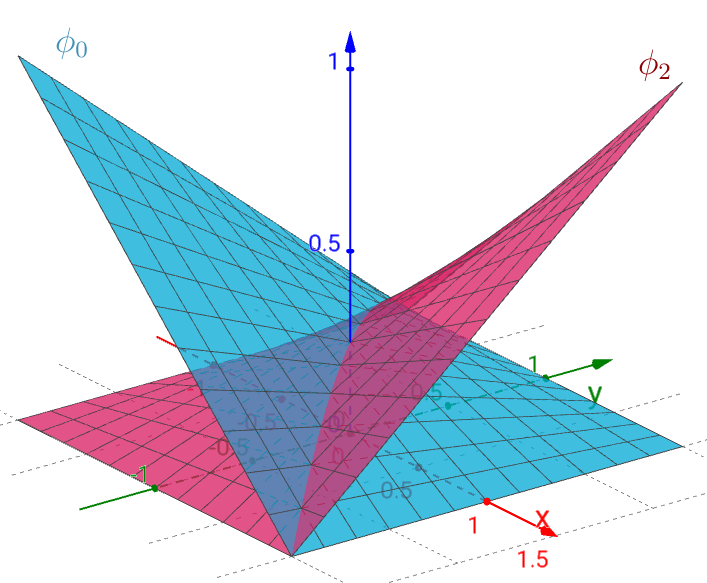
\includegraphics[width=0.4\linewidth]{basis2d_bilinear.png}
\caption{Билинейные функции $\phi_0$, $\phi_2$ в параметрическом квадрате}
\label{fig:basis2d_bilinear}
\end{figure}

\paragraph{Определение двумерных базисов через комбинацию одномерных}
Обратим внимание, что в искомые билинейные базисные функции линейны
в каждом из направлений $\xi, \eta$, если брать их по отдельности.
Значит можно представить эти функции как комбинацию одномерных
линейных базисов \cref{eq:segment_linear_basis} в каждом из направлений.
Узлы двумерного параметрического квадрата можно
выразить через узлы линейного базиса в параметрическом одномерном сегменте,
рассмотренном в п.~\ref{sec:segment_bases}:
$$
\vec \xi_0 = \left(\xi^{1D}_0, \xi^{1D}_0\right), \quad
\vec \xi_1 = \left(\xi^{1D}_1, \xi^{1D}_0\right), \quad
\vec \xi_2 = \left(\xi^{1D}_1, \xi^{1D}_1\right), \quad
\vec \xi_3 = \left(\xi^{1D}_0, \xi^{1D}_1\right).
$$
Значит и соответствующие базисные функции можно выразить
через линейный одномерный базис $\phi^{1D}$ из соотношений \cref{eq:segment_linear_basis}:
\begin{equation*}
\begin{aligned}
\phi_0(\xi, \eta) = \phi_0^{1D}(\xi)\phi^{1D}_0(\eta) = \frac{1-\xi}{2}\frac{1-\eta}{2},\\[5pt]
\phi_1(\xi, \eta) = \phi_1^{1D}(\xi)\phi^{1D}_0(\eta) = \frac{1+\xi}{2}\frac{1-\eta}{2},\\[5pt]
\phi_2(\xi, \eta) = \phi_1^{1D}(\xi)\phi^{1D}_1(\eta) = \frac{1+\xi}{2}\frac{1+\eta}{2},\\[5pt]
\phi_3(\xi, \eta) = \phi_0^{1D}(\xi)\phi^{1D}_1(\eta) = \frac{1-\xi}{2}\frac{1+\eta}{2}.
\end{aligned}
\end{equation*}
Раскрыв скобки можно убедится, что мы получили тот же билинейный базис, что и ранее \cref{eq:quadrangle_bilinear_basis}.

\paragraph{Биквадратичный базис}
Применим этот метод для вычисления биквадратичного базиса, определённого в точках на \figref{fig:quadrangle_basis_points}б.
В качестве основе возьмём квадратичный одномерный базис $\phi^{1D}_i$ из \cref{eq:segment_quadratic_basis}.
\begin{equation}
\label{eq:quadrangle_quadratic_basis}
\begin{array}{ll}
  \phi_0(\xi, \eta) = \phi_0^{1D}(\xi)\phi_0^{1D}(\eta) = \dfrac{\xi^2 - \xi}{2}\dfrac{\eta^2 - \eta}{2},
& \phi_1(\xi, \eta) = \phi_1^{1D}(\xi)\phi_0^{1D}(\eta) = \dfrac{\xi^2 + \xi}{2}\dfrac{\eta^2 - \eta}{2}, \\[10pt]
  \phi_2(\xi, \eta) = \phi_1^{1D}(\xi)\phi_1^{1D}(\eta) = \dfrac{\xi^2 + \xi}{2}\dfrac{\eta^2 + \eta}{2},
& \phi_3(\xi, \eta) = \phi_0^{1D}(\xi)\phi_1^{1D}(\eta) = \dfrac{\xi^2 - \xi}{2}\dfrac{\eta^2 + \eta}{2}, \\[10pt]
  \phi_4(\xi, \eta) = \phi_2^{1D}(\xi)\phi_0^{1D}(\eta) = (1-\xi^2)\dfrac{\eta^2 - \eta}{2},
& \phi_5(\xi, \eta) = \phi_1^{1D}(\xi)\phi_2^{1D}(\eta) = \dfrac{\xi^2 + \xi}{2}(1 - \eta^2),            \\[10pt]
  \phi_6(\xi, \eta) = \phi_2^{1D}(\xi)\phi_1^{1D}(\eta) = (1-\xi^2)\dfrac{\eta^2 + \eta}{2},
& \phi_7(\xi, \eta) = \phi_0^{1D}(\xi)\phi_2^{1D}(\eta) = \dfrac{\xi^2 - \xi}{2}(1 - \eta^2),            \\[10pt]
  \phi_8(\xi, \eta) = \phi_2^{1D}(\xi)\phi_2^{1D}(\eta) = (1-\xi^2)(1 - \eta^2).
&
\end{array}
\end{equation}

\paragraph{Бикубический базис}

\paragraph{Неполный биквадратичный базис}

\paragraph{Неполный бикубический базис}


\section{Алгоритмы}
\subsection{Геометрические алгоритмы}
\subsubsection{Линейная интерполяция}
\begin{figure}[h!]
\centering
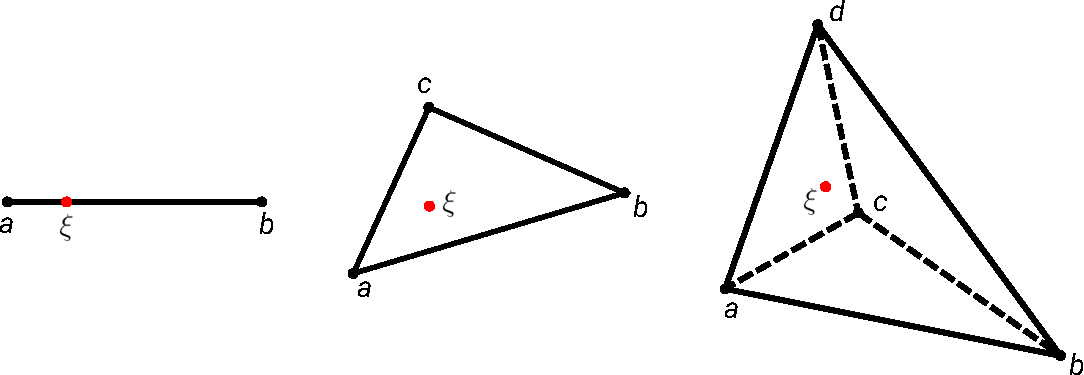
\includegraphics[width=0.8\linewidth]{geom_interp.pdf}
\caption{Порядок нумерации точек одномерного, двумерного и трёхмерного симплекса при линейной интерполяции}
\label{fig:geom_interp}
\end{figure}
Пусть функция $u$ задана в узлах симплекса, имеющего нумерацию согласно рис.~\ref{fig:geom_interp}.
Необходимо найти значение этой функции в точке $\vec \xi$ (эта точка вообще говоря не обязана лежать внутри симлекса).

Интерполяция в одномерном, двумерном и трёхмерном виде запишется как
\begin{align}
\label{eq:simplex_interp_1d}
&u(\xi) =
\frac{
|\triangle_{\xi a}|u(b)+
|\triangle_{b \xi}|u(a)
}
{|\triangle_{ba}|}
\\[10pt]
\label{eq:simplex_interp_2d}
&u(\xi) =
\frac{
|\triangle_{ab\xi}|u(c) +
|\triangle_{bc\xi}|u(a) +
|\triangle_{ca\xi}|u(b)
}
{|\triangle_{abc}|}
\\[10pt]
\label{eq:simplex_interp_3d}
&u(\xi) =
\frac{
|\triangle_{abc\xi}|u(d) +
|\triangle_{cbd\xi}|u(a) +
|\triangle_{cda\xi}|u(b) +
|\triangle_{adb\xi}|u(c)
}
{|\triangle_{abcd}|},
\end{align}
где $|\triangle|$ -- знаковый объём симплекса, вычисляемый как
\begin{align*}
& |\triangle_{ab}| = b - a, \\[10pt]
& |\triangle_{abc}| = \left(\frac{(\vec b - \vec a)\times(\vec c - \vec a)}{2}\right)_z, \\[10pt]
& |\triangle_{abcd}| = \frac{(\vec b - \vec a)\cdot\left((\vec c - \vec a)\times(\vec d - \vec a)\right)}{6}.\\[10pt]
\end{align*}

\subsubsection{Преобразование координат}
\label{sec:coo_transform} 
Рассмотрим преобразование
из двумерной параметрической системы координат $\vec \xi$ 
в физическую систему $\vec x$.
Такое преобразование полностью определяется покоординатными
функциями $\vec x(\vec \xi)$.
Далее получим соотношения, связывающие операции дифференцирования
и интегрирования в физической и параметрической областях.

\subsubsubsection{Матрица Якоби}
Будем рассматривать двумерное преобразование $(\xi, \eta) \to (x, y)$.
Линеаризуем это преобразование (разложим в ряд Фурье до линейного слагаемого)
\begin{align*}
& x(\xi_0 + d\xi, \eta_0 + d\eta) \approx x_0 + \left.\dfr{x}{\xi}\right|_{\xi_0, \eta_0} d\xi
    + \left.\dfr{x}{\eta}\right|_{\xi_0, \eta_0} d\eta, \\
& y(\xi_0 + d\xi, \eta_0 + d\eta) \approx y_0 + \left.\dfr{y}{\xi}\right|_{\xi_0, \eta_0} d\xi
    + \left.\dfr{y}{\eta}\right|_{\xi_0, \eta_0} d\eta,
\end{align*}
где $x_0 = x(\xi_0, \eta_0)$, $y_0 = y(\xi_0, \eta_0)$.
Переписывая это выражение в векторном виде, получим
\begin{equation}
\label{eq:jacobi_linear}
\vec{x}(\vec \xi_0 + \vec{d\xi} ) - \vec{x}_0 = J(\vec \xi_0) \; \vec{d\xi}.
\end{equation}
Матрица $J$ (зависящая от точки приложения в параметрической плоскости) называется матрицей Якоби:
\begin{equation}
\label{eq:jacobi_matrix_2d}
J = \left(
	\begin{array}{cc}
	J_{11} & J_{12}\\[10pt]
	J_{21} & J_{22}\\
	\end{array}
\right)
= \left(
	\begin{array}{cc}
	\ddfr{x}{\xi} & \ddfr{x}{\eta}\\[10pt]
	\ddfr{y}{\xi} & \ddfr{y}{\eta}\\
	\end{array}
\right)
\end{equation}

\paragraph{Якобиан}

\begin{figure}[h!]
\centering
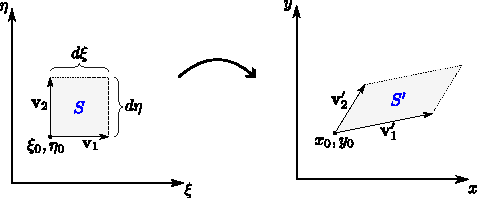
\includegraphics[width=0.6\linewidth]{dxideta.pdf}
\caption{Преобразование элементарного объёма}
\label{fig:dxideta}
\end{figure}

Определитель матрицы Якоби (якобиан), взятый в конкретной точке параметрической плоскости $\vec\xi_0$, показывает,
во сколько раз увеличился элементарный объём около этой точки в результате преобразования.
Действительно, рассмотрим два перпендикулярных элементарных вектора
в параметрической системе координат: $\vec v_1 = (d\xi, 0)$ и $\vec v_2 = (0, d\eta)$
отложенных от точки $\vec\xi_0$ (см.~\figref{fig:dxideta}).
В результате преобразования по формуле \cref{eq:jacobi_linear} 
получим следующие преобразования концевых точек и векторов:
\begin{align*}
& (\xi_0, \eta_0) \to (x_0, y_0), \\
& (\xi_0 + d\xi, \eta_0) \to (x_0 + J_{11} d\xi, y_0 + J_{21} d\xi) \hence \vec v_1 \to \vec v'_1 = (J_{11} d\xi, J_{21} d\xi), \\
& (\xi_0 , \eta_0 + d\eta) \to (x_0 + J_{12} d\eta, y_0 + J_{22} d\eta) \hence \vec v_2 \to \vec v'_2 = (J_{12} d\eta, J_{22} d\eta).
\end{align*}
Элементарный объём равен площади параллелограмма, построенного
на элементарных векторах.
В параметрической плоскости согласно \cref{eq:vec_cross_2d} получим 
$$ |S| = \vec v_1 \times \vec v_2 = d\xi d\eta,$$
и аналогично для физической плоскости:
$$
|S'| = \vec v'_1 \times \vec v'_2 = (J_{11} J_{22} - J_{12} J_{21})d\xi d\eta = |J| d\xi d\eta
$$
Сравнивая два последних соотношения приходим к выводу,
что элементарный объём в результате преобразования увеличился в $|J|$ раз. Тогда можно записать
\begin{equation}
\label{eq:dxdy_dxideta}
dx\,dy = |J|\,d\xi\,d\eta
\end{equation}

Многомерным обобщением этой формулы будет
\begin{equation}
\label{eq:vec_dx_dxi}
d\vec x = |J|\,d\vec \xi
\end{equation}

\subsubsubsection{Дифференцирование в параметрической плоскости}
Пусть задана некоторая функция $f(x, y)$. Распишем её производную по
параметрическим координатам:
\begin{align*}
&\dfr{f}{\xi} = \dfr{f}{x}\dfr{x}{\xi} + \dfr{f}{y}\dfr{y}{\xi}, \\
&\dfr{f}{\eta} = \dfr{f}{x}\dfr{x}{\eta} + \dfr{f}{y}\dfr{y}{\eta}.
\end{align*}
Вспоминая определение \cref{eq:jacobi_matrix_2d}, запишем
\begin{equation*}
\left(\begin{array}{c}
  \ddfr{f}{\xi} \\[10pt]
  \ddfr{f}{\eta}
  \end{array}
\right) = 
J^T 
\left(
  \begin{array}{c}
  \ddfr{f}{x} \\[10pt]
  \ddfr{f}{y}
  \end{array}
\right) =
\left(
  \begin{array}{cc}
    J_{11} & J_{21} \\[10pt]
    J_{12} & J_{22}
  \end{array}
\right)
\left(
  \begin{array}{c}
  \ddfr{f}{\xi} \\[10pt]
  \ddfr{f}{\eta}
  \end{array}
\right)
\end{equation*}
Обратная зависимость примет вид
\begin{equation*}
\left(\begin{array}{c}
  \ddfr{f}{x} \\[10pt]
  \ddfr{f}{y}
  \end{array}
\right) = 
\left(J^T\right)^{-1}
\left(
  \begin{array}{c}
  \ddfr{f}{\xi} \\[10pt]
  \ddfr{f}{\eta}
  \end{array}
\right) =
\frac{1}{|J|}
\left(
  \begin{array}{cc}
    J_{22} & -J_{21} \\[10pt]
    -J_{12} & J_{11}
  \end{array}
\right)
\left(
  \begin{array}{c}
  \ddfr{f}{\xi} \\[10pt]
  \ddfr{f}{\eta}
  \end{array}
\right)
\end{equation*}
В многомерном виде запишем
\begin{equation}
\label{eq:vec_grad_dx}
\nabla_{\vec x} f = \left(J^T\right)^{-1} \nabla_{\vec \xi} f.
\end{equation}

\subsubsubsection{Интегрирование в параметрической плоскости}
Пусть в физической области $\vec x$ задана область $D_x$.
Интеграл функции $f(\vec x)$ по этой области
можно расписать, используя замену \cref{eq:vec_dx_dxi}
\begin{equation}
\label{eq:dxideta_integral}
\int\limits_{D_{x}}f(\vec x)\,d\vec x = \int\limits_{D_{\xi}}f(\vec \xi) \, |J(\vec \xi)|d\vec \xi,
\end{equation}
где $f(\vec \xi) = f(\vec x(\vec \xi))$, а $D_\xi$ -- образ области $D_x$ в параметрической плоскости.

\subsubsubsection{Двумерное линейное преобразование. Параметрический треугольник}
\label{sec:lintri_transform}
\begin{figure}[h!]
\centering
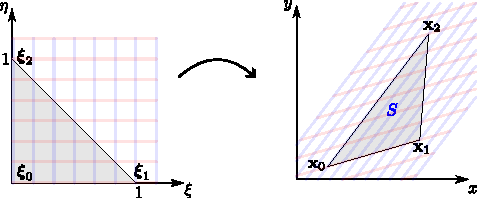
\includegraphics[width=0.6\linewidth]{lintri_transform.pdf}
\caption{Преобразование из параметрического треугольника}
\label{fig:lintri_transform}
\end{figure}
Рассмотрим двумерное преобразование, при котором
определяющие функции являются линейными. То есть представимыми в виде
\begin{align*}
x(\xi, \eta) = A_x \xi + B_x \eta + C_x, \\
y(\xi, \eta) = A_y \xi + B_y \eta + C_y.
\end{align*}
Для определения шести констант, определяющих это преобразование,
достаточно выбрать три любые (не лежащие на одной прямой) точки:
$(\xi_i, \eta_i) \to (x_i, y_i)$ для $i=0,1,2$.
В результате получим систему из шести линейных уравнений (три точки по две координаты),
из которой находятся конcтанты $A_{x,y}, B_{x,y}, C_{x,y}$.
Пусть три точки в параметрической плоскости
образуют единичный прямоугольный треугольник (\figref{fig:lintri_transform}):
\begin{equation*}
\xi_0, \eta_0 = (0, 0),\quad
\xi_1, \eta_1 = (1, 0),\quad
\xi_2, \eta_2 = (0, 1).
\end{equation*}
Тогда система линейных уравнений примет вид
\begin{align*}
&x_0 = C_x,       \quad y_0 = C_y, \\
&x_1 = A_x + C_x, \quad y_1 = A_y + C_y, \\
&y_2 = B_x + C_x, \quad y_2 = B_y + C_y.
\end{align*}
Определив коэффициенты преобразования их этой системы, окончательно запишем преобразование
\begin{equation}
\label{eq:lintri_transform}
\begin{aligned}
&x(\xi, \eta) = (x_1 - x_0)\xi + (x_2 - x_0) \eta + x_0,\\
&y(\xi, \eta) = (y_1 - y_0)\xi + (y_2 - y_0) \eta + y_0.\\
\end{aligned}
\end{equation}
Матрица Якоби этого преобразования \cref{eq:jacobi_matrix_2d}
не будет зависеть от параметрических координат $\xi, \eta$:
\begin{equation}
\label{eq:lintri_jacobi_matrix}
J = \left(
\begin{array}{cc}
x_1 - x_0 & x_2 - x_0 \\
y_1 - y_0 & y_2 - y_0 \\
\end{array}
\right).
\end{equation}
Якобиан преобразования будет равен удвоенной площади треугольника $S$, составленного из определяющих точек в физической плоскости:
\begin{equation}
\label{eq:lintri_jacobian}
|J| = (x_1 - x_0) (y_2 - y_0) - (y_1 - y_0) (x_2 - x_0) = (\vec x_1 - \vec x_0) \times (\vec x_2 - \vec x_0) = 2 |S|.
\end{equation}
Распишем интеграл по треугольнику $S$ по формуле \cref{eq:dxideta_integral}.
Вследствии линейности преобразования якобиан постоянен и, поэтому, его можно вынести его из-под интеграла:
\begin{equation}
\label{eq:lintri_integral}
\int\limits_{S}f(x, y)\,dxdy = |J|\int\limits_0^1 \int\limits_0^{1-\xi} f(\xi, \eta) d\eta d\xi.
\end{equation}

\subsubsubsection{Двумерное билинейное преобразование. Параметрический квадрат}
\label{sec:bilinquad_transform}
\begin{figure}[h!]
\centering
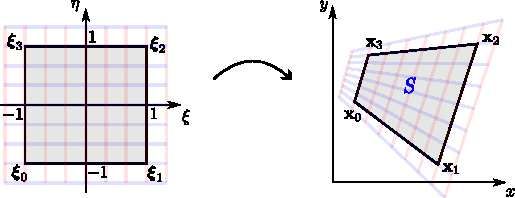
\includegraphics[width=0.6\linewidth]{bilinquad_transform.pdf}
\caption{Преобразование из параметрического квадрата}
\label{fig:bilinquad_transform}
\end{figure}

\subsubsubsection{Трёхмерное линейное преобразование. Параметрический тетраэдр}
TODO

\subsubsection{Свойства многоугольника}
\subsubsubsection{Площадь многоугольника}
\label{sec:polygon_area} 

\begin{figure}[h!]
\centering
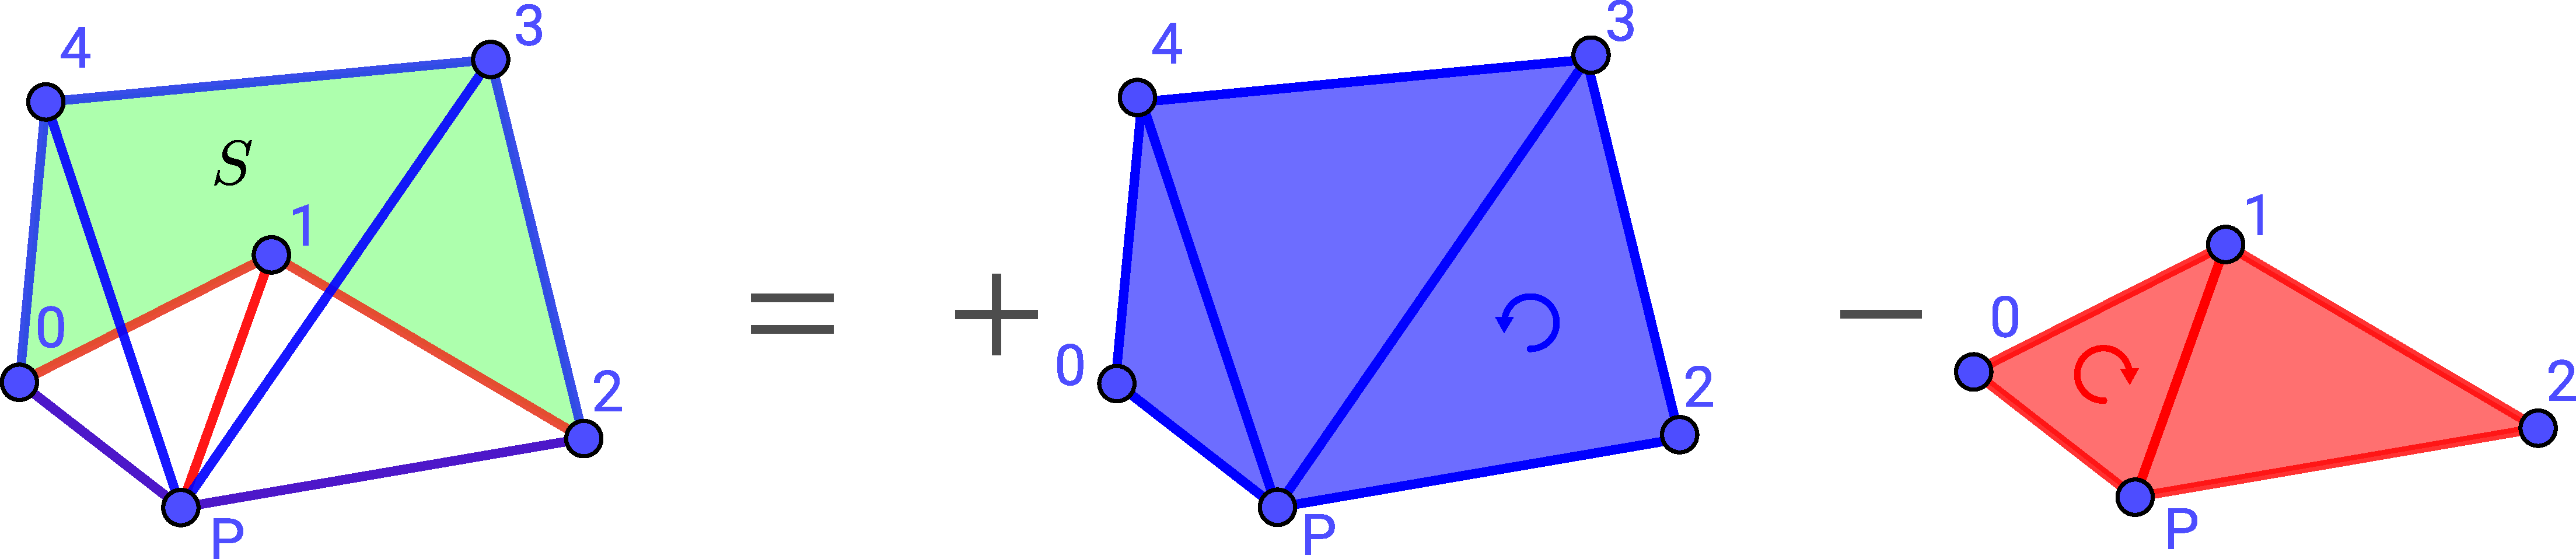
\includegraphics[width=0.7\linewidth]{polygon_area.pdf}
\caption{Площадь произвольного многоугольника}
\label{fig:polygon_area}
\end{figure}

Рассмотрим произвольный несамопересекающийся $N$-угольник $S$,
заданный координатами своих узлов $\vec x_i$, $i=\overline{0, N-1}$,
пронумерованных последовательно против часовой стрелки (\figref{fig:polygon_area}).
Далее введём произвольную точку $\vec p$ и 
от этой точки будем строить ориентированные треугольники до граней многоугольника:
$$
\triangle^p_i = (\vec p, \vec x_i, \vec x_{i+1}), \quad i=\overline{0, N-1},
$$
(для корректности записи будем считать, что $\vec x_N = \vec x_0$).
Тогда площадь исходного многоугольника $S$ будет равна сумме
знаковых площадей треугольников $\triangle^p_i$:
$$
|S| = \sum_{i=0}^{N-1} |\triangle^p_i|, \qquad |\triangle^p_i| = \frac{(\vec x_i - \vec p) \times (\vec x_{i+1} - \vec p)}{2}.
$$
Знак площади ориентированного треугольника зависит от направления закрутки его узлов:
она положительна для закрутки против часовой стрелки и отрицательна, если узлы пронумерованы по часовой стрелке.
В частности, на рисунке~\ref{fig:polygon_area} видно, что треугольники, отмеченные красным: $P01, P12$, будут
иметь отрицательную площадь, а синие треугольники $P23$, $P34$, $P40$ -- положительную. Сумма этих площадей
с учётом знака даст искомую площадь многоугольника.

Для сокращения вычислений воспользуемся произвольностью положения $\vec p$ и совместим
её с точкой $\vec x_0$. Тогда треугольники $\triangle^p_0$, $\triangle^p_{N-1}$
выродятся (будут иметь нулевую площадь).
Обозначим такую последовательную триангуляцию как
\begin{equation}
\label{eq:seq_polygon_triangulation}
\triangle_i = (\vec x_0, \vec x_i, \vec x_{i+1}), \qquad i=\overline{1,N-2}.
\end{equation}
Знаковая площадь ориентированного треугольника будет равна
\begin{equation}
\label{eq:seq_triangle_area}
|\triangle_i| = \frac{(\vec x_i - \vec x_0) \times (\vec x_{i+1} - \vec x_0)}{2}.
\end{equation}
Тогда окончательно формула определения площади примет вид
\begin{equation}
\label{eq:polygon_area}
|S| = \sum_{i=1}^{N-2}|\triangle_i|.
\end{equation}

\paragraph{Плоский полигон в пространтве} Если плоский полигон $S$ расположен в трёхмерном пространстве,
то правая часть формулы \cref{eq:seq_triangle_area} согласно определению векторного произведения в трёхмерном пространстве \cref{eq:vec_cross}
-- есть вектор.
Чтобы получить скалярную площадь, нужно спроецировать этот вектор на единичную нормаль к плоскости
многоугольника:
$$
\vec n = \frac{\vec k}{|\vec k|}, \qquad \vec k = (\vec x_1 - \vec x_0) \times (\vec x_2 - \vec x_0).
$$
Эта формула записана из предположения, что узел $\vec x_2$ не лежит
на одной прямой с узлами $\vec x_0$, $\vec x_1$. Иначе вместо $\vec x_2$ нужно
выбрать любой другой узел, удовлетворяющий этому условию.
Тогда площадь ориентированного треугольника, построенного
в трёхмерном пространстве запишется через смешанное произведение:
\begin{equation}
\label{eq:seq_triangle_area_3d}
|\triangle_i| = \frac{\left((\vec x_i - \vec x_0) \times (\vec x_{i+1} - \vec x_0) \right)\cdot \vec n}{2}.
\end{equation}
Формула для определения площади полигона \cref{eq:polygon_area} будет по прежнему верна.
При этом итоговый знак величины $S$ будет положительным,
если закрутка полигона положительная (против часовой стрелки) при взгляде со стороны
вычисленной нормали $\vec n$.

\subsubsubsection{Интеграл по многоугольнику}
\label{sec:polygon_integral} 
Рассмотрим интеграл функции $f(x,y)$ по $N$-угольнику $S$, заданному последовательными координатами своих узлов $\vec x_i$.
Введём последовательную триангуляцию согласно \cref{eq:seq_polygon_triangulation}.
Тогда интеграл по многоугольнику можно расписать как сумму интегралов по ориентированным треугольникам:
\begin{equation}
\label{eq:seq_triangulation_integral}
\arint{f(x,y)}{S}{xdy} = \sum_{i=1}^{N-2} \arint{f(x,y)}{\triangle_i}{xdy}.
\end{equation}
Далее для вычисления интегралов в правой части
воспользуемся преобразованием к параметрическому треугольнику (п.~\ref{sec:lintri_transform}).
Следуя формуле интегрирования \cref{eq:lintri_integral}, распишем
интеграл по $i$-ому треугольнику:
\begin{equation*}
\arint{f(x,y)}{\triangle_i}{xdy} = |J_i| \int\limits_{0}^{1}\int\limits_{0}^{1-\xi} f_i(\xi, \eta) \, d\eta d\xi,
\end{equation*}
где якобиан $|J_i|$ согласно \cref{eq:lintri_jacobian} есть удвоенная площадь ориентированного треугольника $\triangle_i$
(положительная при закрутке против часовой стрелке и отрицаетельная иначе):
\begin{equation*}
|J_i| = 2|\triangle_i| = (\vec x_i - \vec x_0) \times (\vec x_{i+1} - \vec x_0),
\end{equation*}
а функция $f_i(\xi, \eta)$ есть функция от преобразованных согласно \cref{eq:lintri_transform}
переменных:
\begin{equation*}
f_i(\xi, \eta) = f\left(\left(\vec x_i - \vec x_0\right)\xi + \left(\vec x_{i+1} - \vec x_0\right)\eta + \vec x_0\right).
\end{equation*}
Окончательно запишем
\begin{equation}
\label{eq:polygon_integral}
\arint{f(x,y)}{S}{xdy} = 2 \sum_{i=1}^{N-2}
    |\triangle_i| \int\limits_{0}^{1}\int\limits_{0}^{1-\xi} f_i(\xi, \eta) \, d\eta d\xi.
\end{equation}
Отметим, что эта формула работает и в том случае, когда
полигон расположен в трёхмерном пространстве
(знаковую площадь при этом следует вычислять по \cref{eq:seq_triangle_area_3d}).

\subsubsubsection{Центр масс многоугольника}
\label{sec:polygon_center} 
По определению, координаты центра масс $\vec c$ области $S$ равны среднеинтегральным значениям координатных функций. То есть
\begin{equation*}
c_x = \frac{1}{|S|}\int\limits_{S} x \, dxdy,
\quad 
c_y = \frac{1}{|S|}\int\limits_{S} y \, dxdy.
\end{equation*}
Далее распишем интеграл в правой части через последовательную триангуляцию согласно
\cref{eq:seq_triangulation_integral} с учётом линейного преобразования
\cref{eq:lintri_transform}:
\begin{align*}
\int\limits_{S} x \, dxdy &= \sum_{i=1}^{N-2} \int\limits_{\triangle_i} x \, dxdy\\
                          &= \sum_{i=1}^{N-2} |J_i| \int\limits_0^1\int\limits_0^{1-\xi} ((x_i - x_0)\xi + (x_{i+1} - x_0)\eta + x_0)\, d\eta d\xi\\
                          &= \sum_{i=1}^{N-2} \frac{|J_i|}{2}\frac{x_0 + x_i + x_{i+1}}{3}\\
                          &= \sum_{i=1}^{N-2} |\triangle_i|\frac{x_0 + x_i + x_{i+1}}{3}.
\end{align*}
Итого, с учётом \cref{eq:polygon_area}, координаты центра масс примут вид
\begin{align*}
&\vec c = \dfrac{\displaystyle\sum_{i=1}^{N-2} \dfrac{\vec x_0 + \vec x_i + \vec x_{i+1}}{3}|\triangle_i|}{\displaystyle\sum_{i=1}^{N-2} |\triangle_i|}.
\end{align*}
Если полигон расположен в двумерном пространстве $xy$, то знаковая площадь треугольников
вычисляется по формуле \cref{eq:seq_triangle_area}.
В случае трёхмерного пространтва должна использоваться формула \cref{eq:seq_triangle_area_3d}.

\subsubsection{Свойства многогранника}
\subsubsubsection{Объём многогранника}
\label{sec:polyhedron_volume} 
TODO
\subsubsubsection{Интеграл по многограннику}
\label{sec:polyhedron_integral} 
TODO
\subsubsubsection{Центр масс многогранника}
\label{sec:polyhedron_center} 
TODO

\subsubsection{Поиск многоугольника, содержащего заданную точку}
TODO

\subsection{Форматы хранения разреженных матриц}
\label{sec:sparse-matrix}
\subsubsection{CSR-формат}
\label{sec:csr}
При реализации решателей систем сеточных уравнений важно учитывать
разреженный характер используемых в левой части матриц. То есть избегать
хранения и ненужных операций с нулевыми элементами матрицы.

Здесь будем рассматривать общие форматы хранения, не привязанные к конкретному шаблону.
Любой общий формат хранения должен хранить
информацию о шаблоне матрице (адресах ненулевых элементов)
и значениях матричных коэффициентов в этом шаблоне.

В CSR (Compressed sparse rows) формате
все ненулевые элементы хранятся в линейном массиве \ename{vals}.
А шаблон матрицы -- в двух массивах
\begin{itemize}
	\item массиве колонок \ename{cols} -- значений колонок для соответствующих ему значений из массива \ename{vals},
	\item массиве адресов \ename{addr} -- индексах массива \ename{vals}, с которых начинается описание соответствующей строки.
\end{itemize}
В конце массива \ename{addr} добавляется общая длина массива \ename{vals}.

Таким образом, длины массивов \ename{vals}, \ename{cols} равны количеству ненулевых элементов матрицы,
а длина массива \ename{addr} равна количеству строк в матрице плюс один.

Для облегчения процедур поиска описание каждой строки должно идти последовательно
с увеличением индекса колонки.

Для примера рассмотрим следующую матрицу
\begin{equation}
\label{eq:example-sparse-matrix}
\left(
\begin{array}{cccc}
2.0 & 0 & 0 & 1.0 \\
0 & 3.0 & 5.0 & 4.0 \\
0 & 0 & 6.0 & 0 \\
0 & 7.0 & 0 & 8.0 \\
\end{array}
\right)
\end{equation}

Массивы, описывающие матрицу в формате CSR примут вид

\begin{equation*}
\begin{array}{r|l|l|l|l|l}
      & row=0     & row=1          & row=2& row=3&\\
\hline
vals= & 2.0, 1.0, & 3.0, 5.0, 4.0, & 6.0, & 7.0, 8.0 &\\
\hline
cols= & 0,\phantom{.0} 3,\phantom{.0}      & 1,\phantom{.0}2,\phantom{.0}3,\phantom{.0}          & 2,\phantom{.0}   & 1,\phantom{.0} 3     &\\
\hline
addr= & 0,        & 2,             & 5,   & 6,       & 8 \\
\hline
\end{array}
\end{equation*}

Рассмотрим реализацию базовых алгоритмов для матриц, заданных в этом формате.

Пусть матрица задана следующими массивами:
\begin{minted}[linenos=false]{c++}
std::vector<double> vals; // массив значений
std::vector<size_t> cols; // массив столбцов
std::vector<size_t> addr; // массив адресов
\end{minted}

Число строк в матрице:
\begin{minted}[linenos=false]{c++}
size_t nrows = addr.size()-1;
\end{minted}

Число элементов в шаблоне (ненулевых элементов)
\begin{minted}[linenos=false]{c++}
size_t n_nonzeros = vals.size();
\end{minted}

Число ненулевых элементов в заданной строке `irow`
\begin{minted}[linenos=false]{c++}
size_t n_nonzeros_in_row = addr[irow+1] - addr[irow];
\end{minted}

Умножение матрицы на вектор `v` (длина этого вектора должна быть равна числу строк в матрице).
Здесь реализуется суммирование вида
\begin{equation*}
    r_i = \sum_{j=0}^{N-1} a_{ij} v_j,
\end{equation*}
при этом избегаются лишние операции с нулями
\begin{minted}[linenos=false]{c++}
// число строк в матрице и длина вектора v
size_t nrows = addr.size() - 1;
// массив ответов. Инициализируем нулями
std::vector<double> r(nrows, 0);
// цикл по строкам
for (size_t irow=0; irow < nrows; ++irow){
	// цикл по ненулевым элементам строки irow
	for (size_t a = addr[irow]; a < addr[irow+1]; ++a){
		// получаем индекс колонки
		size_t icol = cols[a];
		// значение матрицы на позиции [irow, icol]
		double val = vals[a];
		// добавляем к ответу
		r[irow] += val * v[icol];
	}
}
\end{minted}


Поиск значения элемента матрицы по адресу \cvar{(irow, icol)} с учётом локально сортированного вектора \cvar{cols}
\begin{minted}[linenos=false]{c++}
using iter_t = std::vector<size_t>::const_iterator;
// указатели на начало и конец описания строки в массиве cols
iter_t it_start = cols.begin() + addr[irow];
iter_t it_end = cols.begin() + addr[irow+1];
// поиск значения icol в отсортированной последовательности [it_start, it_end)
iter_t fnd = std::lower_bound(it_start, it_end, icol);
if (fnd != it_end && *fnd == icol){
	// если нашли, то определяем индекс найденного элемента в массиве cols
	size_t a = fnd - cols.begin();
	// и возвращаем значение из vals по этому индексу
	return vals[a];
} else {
	// если не нашли, значит элемент [irow, icol] находится вне шаблона. Возвращаем 0
	return 0;
}
\end{minted}

Формат CSR обеспечивает максимальную компактность хранения
разреженной матрицы и при этом удобен для последовательной итерации по элементам матрицы (операции умножения матрицы на вектор),
но его существенным недостатком является высокая сложность добавления нового элемента в шаблон.

\subsubsection{Массив словарей}
\label{sec:lodmat}
При реализации сеточных методов решения дифференциальных уравнений работу с матрицами
можно разбить на два этапа: сборка матриц и их непосредственное использование.
Сборка матрицы в свою очередь может быть разделена на
этап вычисление шаблона матрицы (символьная сборка) и
непосредственное вычисление коэффициентов матрицы (числовая сборка).

На этапе использования матрицы основной операцией
является умножение матрицы на вектор, где наиболее эффективным является CSR-формат.

В случае использования неструктурированных сеток этап символьной сборки
является нетривиальной операцией и сводится к неупорядоченному добавлению
новых элементов в шаблон матрицы. Как было отмечено ранее, 
такая операция в случае использования CSR формата неэффективена.

Поэтому часто для этапов сборки и расчёта используют
разные форматы хранения матриц, первый из которых оптимизирован для операции вставки, а второй -- для операции умножения на вектор.
В качестве формата, оптимизированного для вставки, можно представить формат массива словарей (List of dictionaries), где каждая строка матрицы
описывается словарём, ключём которого является индекс колонки, а значением -- величина соответствующего матричного коэффициента.

С использованием синтаксиса C++ такой формат может быть описан следующим образом:
\begin{cppcode}
std::vector<std::map<size_t, double>> data;
\end{cppcode}

Марица вида \eqref{eq:example-sparse-matrix} в таком формате примет вид
\begin{cppcode}
data = {
	{0: 2.0, 3: 1.0},
	{1: 3.0, 2: 5.0, 3: 4.0},
	{2: 6.0},
	{1: 7.0, 3: 8.0}
};
\end{cppcode}

Добавление нового матричного коэффициента сведётся к вставке элемента в словарь:
\begin{cppcode}
data[i][j] = value;
\end{cppcode}

А основной операцией для такого формата будет служить
конверсия в CSR:
\begin{cppcode}
std::vector<size_t> addr{0};
std::vector<size_t> cols;
std::vector<double> vals;
for (size_t irow=0; irow < data.size(); ++irow){
	for (auto it: data[irow]){
		cols.push_back(it.first);
		vals.push_back(it.second);
	}
	addr.push_back(addr.back() + data[irow].size());
}
\end{cppcode}
Поскольку данные в контейнере типа \cvar{std::map} итерируются
в отсортированном по ключам порядке, то полученный
в результе массив \cvar{cols} также является локально отсортированным.

\subsection{Методы решения систем уравнений}
Будем рассматривать систему 
\begin{equation}
\label{eq:sae_generic}
\mat A u = f.
\end{equation}

\subsubsection{Простые итерационные алгоритмы}
\label{sec:sae_simple}
\subsubsubsection{Метод Якоби}
\label{sec:sae_jacobi}
Будем рассматривать систему уравнений вида
\begin{equation*}
    \sum_{j=0}^{N-1} A_{ij} u_j = r_i, \quad i = \overline{0, N-1}
\end{equation*}
относительно неизвестного сеточного вектора $\{u\}$.

В классическом виде алгоритм Якоби формулируется в виде
\begin{equation*}
    \hat u_i = \frac{1}{A_{ii}}\left(r_i - \sum_{j\neq i} A_{ij}{u_j}\right)
\end{equation*}

Произведём некоторые преобразования
\begin{align*}
    \hat u_i &= \frac{1}{A_{ii}}\left(r_i - \sum_{j} A_{ij}{u_j} + A_{ii}u_i\right) \\
             &= u_i + \frac{1}{A_{ii}}\left(r_i - \sum_{j} A_{ij}{u_j}\right)
\end{align*}

Таким образом, программировать итерацию этого алгоритма, обновляющую значения массива $\{u\}$, можно в виде
\begin{align*}
    &\check u = u; \\
    &\textbf{for } i=\overline{0, N-1} \\ 
    &\quad u_i \mathrel{{+}{=}} \frac{1}{A_{ii}}\left(r_i - \sum_{j=0}^{N-1} A_{ij}{\check u_j}\right)\\
    &\textbf{endfor} \\
\end{align*}

\subsubsubsection{Метод Зейделя}
\label{sec:sae_seidel}

Формулируется в виде
\begin{equation*}
    \hat u_i = \frac{1}{A_{ii}}\left(r_i - \sum_{j<i} A_{ij}{\hat u_j} - \sum_{j>i} A_{ij}{u_j} \right).
\end{equation*}

Поскольку этот метод неявный относительно уже найденных на итерации значений, то в отличии от метода Якоби этот алгоритм не требует создания временного массива $\hat u$
при программировании. Псевдокод для реализации итерации этого метода можно записать как

\begin{align*}
    &\textbf{for } i=\overline{0, N-1} \\ 
    &\quad u_i \mathrel{{+}{=}} \frac{1}{A_{ii}}\left(r_i - \sum_{j=0}^{N-1} A_{ij}{u_j}\right)\\
    &\textbf{endfor}
\end{align*}


\subsubsubsection{Метод последовательных верхних релаксаций SOR}
\label{sec:sae_sor}

Этот метод основан на добавлении к решению результатов итераций Зейделя с
коэффициентом $\omega > 1$. То есть он изменияет решение по тому же
принципу, что и метод Зейделя, но искуственно увеличивает эту добавку.

Формулируется этот метод в виде
\begin{equation*}
    \hat u_i = (1-\omega) u_i + \frac{\omega}{A_{ii}}\left(r_i - \sum_{j<i} A_{ij}{\hat u_j} - \sum_{j>i} A_{ij}{u_j} \right).
\end{equation*}
Для устойчивости метода необходимо $\omega < 2$. В частности, для одномерных задач,
заданных на единичном отрезке, для оптимальной сходимости можно использовать соотношение $\omega \approx 2 - 5 h$,
где $h$ -- шаг сетки.

Итерация этого метода по аналогии с методом Зейделя может быть запрограммирована в виде

\begin{align*}
    &\textbf{for } i=\overline{0, N-1} \\ 
    &\quad u_i \mathrel{{+}{=}} \frac{\omega}{A_{ii}}\left(r_i - \sum_{j=0}^{N-1} A_{ij}{u_j}\right)\\
    &\textbf{endfor}
\end{align*}

\subsubsection{Метод коррекции поправки}
\label{sec:it_def_corr}
Пусть $u^n$ -- некоторое приближённое решение системы \cref{eq:sae_generic} на итерационном слое.
Введём невязки как
\begin{equation}
\label{eq:sae_rn}
r^n = f - \left(\mat A u\right)^n
\end{equation}
и поправку для перехода на следующий итерационный слой:
\begin{equation*}
\triangle u^n = u^{n+1} - u^{n}.
\end{equation*}
Обобщённый процесс с предобуславливателем $\mat B$ для исходной системы можно записать в виде
\begin{equation}
\label{eq:sae_un_problem}
\mat B \triangle u^n = r^n
\end{equation}

Этот процесс является согласованным: если в качестве $u^n$ взять точное решение системы \cref{eq:sae_generic},
то $r^n = 0$, и следовательно, $\triangle u^n = 0$.

Алгоритм решения исходной системы будет иметь следующий вид:
\begin{enumerate}
\item задать начальное приближение $u^n$ при $n=0$
\item вычислить невязку $r^n$ из \cref{eq:sae_rn}
\item если норма невязки $||r^n|| < \epsilon$, то завершить итерации
\item решив систему \cref{eq:sae_un_problem} получить поправку $\triangle u^n = \mat B^{-1} r^n$.
\item найти следующее приближение $u^{n+1} = u^{n} + \triangle u^{n}$
\item увеличить счётчик $n = n + 1$ и перейти на шаг 2.
\end{enumerate}

Конкретный итерационный метод целиком определяется выбором предобуславливаетеля.
В качестве предобуславливателя обычно выбирают матрицу, похожую на $\mat A$, но при этом легкообратимую.
Некоторые примеры:
\begin{itemize}
\item если выбрать константу $B = 1/\gamma$, то получим
простой итерационный процесс Ричардсона с шагом $\gamma$.
\item диагональная часть исходного оператора $B = \{a_{ii}\}$ приводит к методу Якоби \secref{sec:sae_jacobi}
\item нижняя треугольная часть исходной матрицы $B = \{a_{ij}\}, j\leq i$ даёт метод Зейделя \secref{sec:sae_seidel}.
\end{itemize}

Если в качестве предобуславливателя взять изходную матрицу $\mat A$, 
то итерационный процесс сойдётся за одну итерацию. Действительно из \cref{eq:sae_rn,eq:sae_un_problem}:
\begin{equation*}
u^{n+1} = u^{n} + A^{-1}(f - A u^n) = A^{-1} f
\end{equation*}

Это метод требует прямого обращения только предобуславливаетеля $\mat B$, но не 
исходного оператора $\mat A$, поэтому он может быть применён в том числе и для решения нелинейных систем.

Для обращения самого предобуславливателя в свою очередь так же может
быть использован итерационный алгоритм. Этот итерационный процесс будет являться
внутриннем, поэтому не будет требовать глубокой сходимости.
Зачастую для обращения предобуславливателя достаточно сделать 2-3 поверхностные итерации
одним из простых методов из \secref{sec:sae_simple}.

\subsubsection{Методы подпространств Крылова}

\subsubsubsection{Итерационный процесс BiCGStab с предобуславливателем}
\label{sec:bicgstab}

Инициализация
\begin{enumerate}
\item есть начальное приближение $u^0$
\item вычисляем невязку
$$r_0 = f - \mat A u_0$$
\item предобуславливаем невязку
$$r_0' = \matinv{M}r_0$$
\item запоминаем начальную невязку
$$\tilde r = r_0'$$
\item инициализируем
$$p_0' = v_0' = 0, \quad \rho_0 = \omega_0 = \alpha_0 = 1.0$$
\end{enumerate}

Далее на $k$-ой итерации

\begin{enumerate}
\item проецируем текущую невязку на начальную
$$\rho_k = \tilde r^T \cdot r'_{k-1}$$
\item коэффициент $\beta$:
$$\beta_k = \frac{\rho_k}{\rho_{k-1}} \frac{\alpha_{k-1}}{\omega_{k-1}}$$
\item Обновляем направление
$$p'_k = r'_{k-1} + \beta_k \left( p'_{k-1} - \omega_{k-1} v'_{k-1} \right)$$
\item
$$v_k'=\matinv{M}\mat A p_k'$$
\item коэффициент $\alpha$
$$\alpha_k = \frac{\rho_k}{\tilde r^T \cdot v'_k}$$
\item Промежуточный вектор $s$:
$$s'_k =  r'_{k-1} - \alpha_k v'_k$$
\item Промежуточный вектор $t$
$$t'_k = \matinv{M}\mat{A}s_k'$$
\item множитель $\omega$
$$\omega_k = \frac{ (t_k')^T \cdot s'_k} { (t_k')^T \cdot t_k' }.$$
\item обновляем невязку и решение
\begin{equation}
\label{eq:schwarz_bicgstab}
\begin{aligned}
& u_k = u_{k-1} + \alpha_k p'_k + \omega_k s'_k, \\
& r'_k = s'_k - \omega_k t'_k
\end{aligned}
\end{equation}
\end{enumerate}


\section{Работа с инфраструктурой проекта CFDCourse}
В настоящем параграфе будут даны инструкции для разворачивания инфраструктуры сборки проекта
для операционных систем Linux(Ubuntu), MacOS и Windows.

В процессе настройки будет необходимо установить систему контроля версий {\bf Git},
систему контейнеризации {\bf Docker} и (опционально) интегрированную среду разработки.
Проект позволяет работать в любой среде разработки.
Ниже будут приведены инструкции для настройки {\bf vscode}.

Процесс сборки и запуска программ будет осуществляться в системе, развёрнутой в докере на основе Ubuntu 24.04.
В дальнейшем систему, установленную непосредственно на компьютере, будем называть хост системой.
А систему, развёрнутую в докере -- контейнером.

Для успешной установке на хосте должно быть около 5Гб свободного места.

\subsection{Клонирование}
Для клонирования проекта на локальный компьютер необходимо установить систему контроля версий Git
и открыть терминал на хост-системе в папке, в которой планируется хранить папку с репозиторием.
В нижеследующих инструкциях в качестве такой папки будет использоваться домашняя папка пользователя.

\begin{center}

\begin{tcolorbox}[osstyle, title=Ubuntu]
Откройте терминал и в нём
\begin{shelloutput}
sudo apt install git  # установка гита
cd ~                  # переходим в папку,
                      # где будет хранится папка с репозиторием
\end{shelloutput}
\end{tcolorbox}

\begin{tcolorbox}[osstyle, title=Windows]
В Windows необходимо скачать и установить дистрибутив
\url{https://github.com/git-for-windows/git/releases/download/v2.51.0.windows.1/Git-2.51.0-64-bit.exe}.
Далее откройте командную строку \ename{cmd}. И в ней перейдите в целевую папку
\begin{shelloutput}
cd %USERPROFILE%
\end{shelloutput}
\end{tcolorbox}

\begin{tcolorbox}[osstyle, title=MacOs]
Откройте терминал и в нём
\begin{shelloutput}
# Установите Homebrew, если у вас его ещё нет
/bin/bash -c \
"$(curl -fsSL https://raw.githubusercontent.com/Homebrew/install/HEAD/install.sh)"
# установка гита
brew install git
# переходим в папку где будет хранится папка с репозиторием
cd ~                  
\end{shelloutput}
\end{tcolorbox}

\end{center}

Далее необходимо клонировать репозиторий

\begin{shelloutput}
git clone https://github.com/kalininei/CFDCourse27
\end{shelloutput}

В результате в домашней папке должна появиться папка с \ename{CFDCourse27}.

\subsection{Разворачивание контейнера}

Установим докер

\begin{tcolorbox}[osstyle, title=Ubuntu+apt]
Запустить скрипт, написанный на основе инструкций с официального сайта \url{https://docs.docker.com/engine/install/ubuntu/#install-using-the-repository}:
\begin{shelloutput}
cd ~/CFDCourse27    # перейдём в репозиторий
./scripts/ubuntu_docker_install.sh
\end{shelloutput}
\end{tcolorbox}

\begin{tcolorbox}[osstyle, title=Windows/MacOs+DockerDesktop]
Скачайте и установите дистрибутив с официального сайта 
\begin{itemize}
\item \url{https://docs.docker.com/desktop/setup/install/windows-install/} для Windows
\item \url{https://docs.docker.com/desktop/setup/install/mac-install/} для MacOs
\end{itemize}
Далее следуйте процедуре установки десктопного приложения.
После установки запустите \ename{DockerDesktop}.
Этап регистрации при запуске опционален и может быть пропущен.
\end{tcolorbox}

Далее в терминале находясь в директории \ename{CFDCourse27} развернём контейнер:
\begin{shelloutput}
docker compose up --build -d
\end{shelloutput}
Если вы работаете на Unix-системе с несколькими пользователями и ваш пользователь не является дефолтным, то лучше собрать контейнер под своим пользовательским id. Для этого нужно определить необходимые переменные окружения выполнив вместо последней команды из предыдущего листинга:
\begin{shelloutput}
USER_ID=$(id -u) GROUP_ID=$(id -g) docker compose up --build -d
\end{shelloutput}
Альтернативно можно перестраивать контейнер, запуская с хост системы скрипт \ename{scripts/rebuild_container.sh}.

На этом этапе будет скачаны необходимые образы и запущен контейнер.
По окончании можно убедиться, что контейнер работает
\begin{shelloutput}
docker ps
\end{shelloutput}
В случае работы с \ename{DockerDesktop} запущенный контейнер будет виден в графическом интерфейсе во вкладке \ename{Containers}.

\subsection{Базовая разработка}
\label{sec:howto_basic_dev}
Чтобы скомпилировать проект необходимо войти в терминал контейнера.
Далее
\begin{shelloutput}
docker ps                   # Убедимся, что контейнер cfd27 запущен
docker exec -it cfd27 bash  # Войдём в него
\end{shelloutput}

На Unix системе можно использовать скрипт \ename{scripts/attach_to_container.sh}.

Папка хоста с репозиторием \ename{CFDCourse} примонтирована к папке контейнера \ename{/app}.
Войдём туда
\begin{shelloutput}
cd /app   # заходим в директорию
ls -alh   # смотрим список файлов
\end{shelloutput}
Для удобства в контейнере установлен консольный файловый менеджер \ename{mc},
который можно использовать для операций с файлами. Так же есть его псевдоним \ename{mcc},
который отличается от базового \ename{mc} тем, что запоминает текущую директорию при выходе.
Благодаря чему его можно использовать для навигации вместо \ename{cd}.


\subsubsection{Особенности проекта}
\begin{itemize}
\item Проект состоит из статически линкуемой библиотеки \ename{libcfd27.a} и исполняемого файла \ename{cfd27_test} с тестовыми программами для этой библиотеки.
      Исходники библиотеки лежат в директории \ename{src/cfd}, исходники тестов -- \ename{src/test},
\item Используется 23-ый стандарт C++,
\item Сборка осуществляется в системе cmake,
\item Для написания тестов используется фреймворк \ename{Catch2},
\item В проекте установлены жёсткие правила работы с предупреждениями компилляции, из-за которых они как обрабатываются ошибки,
\item В проекте установлены форматтеры для исходных кодов на С++, python, cmake. При сохранении любого исходного файла этих форматов в vscode
      форматтер будет вызван автоматически. Если исходники модифицировались иначе, то запустить форматтер для всех файлов проекта
      можно скриптом \ename{scripts/formatall.sh} из папки \ename{/app}.
\end{itemize}

\subsubsection{Сборка в отладочном режиме}
Из папки \ename{/app} контейнера:
\begin{shelloutput}
mkdir build                        # создаём папку, в которую будут строится программа
cd build                           # Заходим
cmake .. -DCMAKE_BUILD_TYPE=Debug  # Строим сборочные скрипты
make -j4                           # Компилируем на 4-х потоках
\end{shelloutput}
Сама папка \ename{build} является временной папкой для построения.
Она не подключена к системе контроля версий.  И может быть удалена и создана заново (например для полной гарантированной очистки кэша построения).
Бинарные файлы будут построены в папку \ename{/app/build/bin}.
Для запуска тестов зайдём в эту папку:
\begin{shelloutput}
cd bin
./cfd27_test                # запуск всех тестов
./cfd27_test [grid1]        # запуск единственного тест кейса
\end{shelloutput}

\subsubsection{Сборка в релизном режиме}
\label{sec:debug_build}
Отличается от сборки в отладочном режиме только флагом \ename{cmake}.
Будем строить в папку \ename{build_release}.
Также от папки \ename{/app}
\begin{shelloutput}
mkdir build_release                         # создаём папку
cd build_release                            # Заходим
cmake .. -DCMAKE_BUILD_TYPE=RelWithDebInfo  # Или просто Release,
                                            # если отладочная информация не нужна
make -j4                                    # Компилируем на 4-х потоках
cd bin                                      # заходим в папку с исполняемым файлом
./cfd27_test                                # запуск всех тестов
./cfd27_test [grid1]                        # запуск единственного тест кейса
\end{shelloutput}

\subsubsection{Работа с кодом}
Работать с исходными файлами можно находясь на хосте и используя любой удобный текстовый редактор.
(например \ename{notepad++} на Windows).
Порядок работы будет выглядеть следующим образом
\begin{itemize}
\item Редактировать исходные файлы на хосте в папке \ename{CFDCourse27/src}
\item Для сборки переключиться на терминал и выполнить вышеописанную процедуру сборки
\item Если сборка не прошла из-за ошибок в коде, эти ошибки будут распечатаны в терминал с указанием файла и номера строки
\item Для отладки можно использовать консольный отладчик \ename{gdb} из терминала
\end{itemize}

\subsection{Разработка в vscode}
\subsubsection{Подключение к контейнеру}
Необходимо установить vscode на хосте следуя инструкциям с официального сайта \url{https://code.visualstudio.com/Download}.
В самом vscode нужно установить расширение \ename{Remote Explorer, Dev Containers} для удалённой разработки в контейнере. 
Далее нужно переключиться на вкладку RemoteExplorer (см. рис.~\ref{fig:vscode_to_docker}).

\begin{figure}[h]
\centering
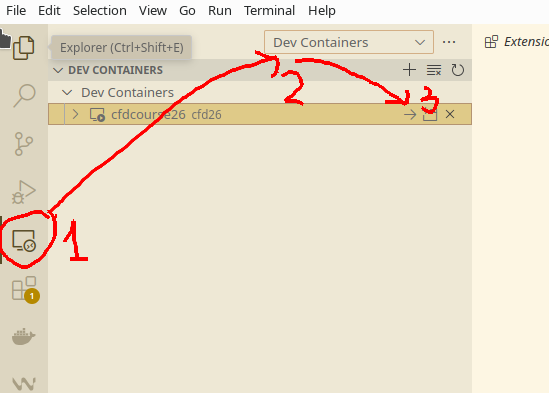
\includegraphics[width=0.6\linewidth]{attach_vscode_to_docker.png}
\caption{Подключения vscode к контейнеру}
\label{fig:vscode_to_docker}
\end{figure}

\subsubsection{Настройки vscode}
Далее необходимо открыть папку \ename{/app}: \ename{File->Open Folder...}.
Контейнер содержит в себе базовые настройки vscode, которые при сборке контейнера
копируются в папки \ename{.vscode, .vscode-server}.

Следует отметить, что удалённо подключённый vscode не может пользоваться
расширениями, установленными на хосте. Все необходимые расширения нужно устанавливать в контейнер заново.
Список базовых расширений, необходимых для работы, уже содержится в настроечных файлах.
Когда вы откроете папку \ename{app} в vscode, вам будет предложено эти расширения установить. Нужно согласиться.

Настроечные папки \ename{.vscode, .vscode-server} игнорируются системой контроля версий и расположены на хосте.
То есть вы можете дополнительно установить туда любые свои расширения и донастроить vscode как вам удобно.
Эти настройки не будут зависеть от ветки гита и не будут затираться при пересборке контейнера.

Если всё же понадобится обнулить настройки vscode, нужно
\begin{enumerate}
\item удалить папки \ename{.vscode, .vscode_server}
\item удалить все настройки из конфигурационного файла контейнера (\ename{ctrl+shift+p, open container configuration file})
\item выйти из контейнера на vscode: \ename{File->Close Remote Connection}
\item остановить и пересобрать контейнер на хосте
\begin{shelloutput}
docker stop cfd27
docker compose up --build -d
\end{shelloutput}
\end{enumerate}

\subsubsection{Сборка и отладка}
\label{sec:build_vscode}
В папке \ename{.vscode} лежат базовые таски и лаунчи для компилляции и запуска программы.
В случае необходимости можете дополнить базовый набор своими командами.
Согласно настройкам по умолчанию
по нажатию \ename{F5} происходит сборка программы в отладочном режиме и запуск отладки
тестовой программы с прогоном всех тестов.
Посмотреть результаты можно на вкладке \ename{TERMINAL}.
В случае ошибок компилляции, список этих ошибок будет виден на вкладке \ename{PROBLEMS}.

Для отладки конкретного теста необходимо запустить тестовую программу с аргументом (например \cvar{cfd27_test [grid1]}.
Чтобы передать программе аргумент нужно этот аргумент прописать в файле \ename{.vscode/launch.json}
в поле \ename{args}. Либо создать ещё одну конфигурацию запуска с вашими аргументами и указать эту конфигурацию в настройке \ename{Run And Dubug}.

Чтобы собрать программу без запуска нужно выполнить таск (\ename{ctrl+shift+b}): \ename{cmake: build debug, cmake: build release}
для отладочного и релизного режима соответственно. 

В целом сборка на vscode представляет из себя автоматизированный алгоритм, представленный в п.~\ref{sec:howto_basic_dev}.
То есть исполняемая программа в дебаговой версии кладётся в папку \ename{build}, в релизной -- в \ename{build_release} и её можно запустить из терминала.
Удаление этих папок ведёт к полной очистке кэша построения.


\subsection{Работа с системой контроля версий}
Работать с гитом можно как с хоста (из папки \ename{CFDCourse27}),  так и из контейнера (из папки \ename{\app}).
Ниже будут даны инструкции для работы с гитом в консоли.
Альтернативно, можно установить графический интерфейс (например \ename{GitExtensions} для Windows)
или командами vscode на вкладке \ename{Source Control}.

Из системы контроля версий исключены следующие каталоги:
\begin{itemize}
\item build*/   -- папки со сборками,
\item .vscode, .vscode-server -- настройки и рисширения vscode,
\item local\_data -- папка для хранения любых пользовательских данных.
\end{itemize}
Изменения из этих папках не будут отслежены и скоммичены.

\subsubsection{Порядок работы с репозиторием CFDCourse}

Основная ветка проекта -- \ename{main}. После каждой лекции в эту ветку будет отправлен коммит с сообщением \ename{lect{index}}.
В этом коммите будет дополнен pdf документ с содержанием лекции, задание по итогам лекции и необходимые для этого задания изменения в коде.

\subsubsubsection{Получение последнего коммита}
Таким образом, {\bf после лекции}, после того, как изменение \ename{lect{index}} придёт на сервер, необходимо выполнить следующие команды
\begin{shelloutput}
git checkout main    # перейти на основную ветку
git pull             # получить изменения
\end{shelloutput}

Если изменения не содержали никаких изменений в настроечных файлах контейнера \ename{Dockerfile, docker-compose.yaml},
то для сборки проекта рестарт контейнера не требуется.
Иначе требуется пересобрать контейнер:
\begin{shelloutput}
docker stop cfd27            # остановить текущий контейнер
docker compose up --build -d # пересобрать новый
\end{shelloutput}

\subsubsubsection{Создание коммита с текущим дз}
После того, как была сделана какая то работа по заданиям,
\begin{shelloutput}
git checkout -b hw-lect{index}      # создать локальную ветку, содержащую задание
git add .
git commit -m "{свой комментарий}"  # скоммитить свои изменения в эту ветку
\end{shelloutput}

Даже если задание выполнено не до конца, вы в любой момент можете переключиться на ветку с заданием и его доделать
\begin{shelloutput}
git checkout hw-lect{index}
\end{shelloutput}

\subsection{Paraview}
\label{sec:paraview}

\subsubsection{Данные на одномерных сетках}
\label{sec:paraview-1d}

Заданные на сетке данные паравью показывает цветом.
Поэтому при загрузке одномерных сеток можно видеть картинку типа
\begin{center}
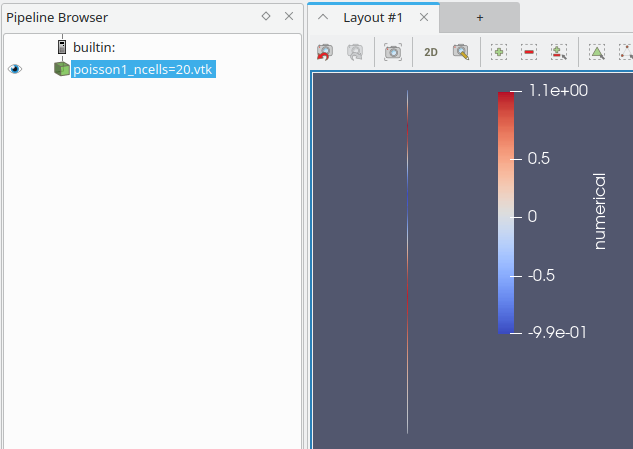
\includegraphics[width=0.5\linewidth]{howto_paraview_1d_1.png}
\end{center}
\paragraph{Развернуть изображение в плоскость xy}
\begin{center}
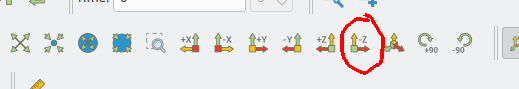
\includegraphics[width=0.5\linewidth]{howto_paraview_1d_2.png}
\end{center}
\paragraph{Отобразить данные в виде y-координаты} Для того, что бы данные отображались в качестве значения по оси ординат, к загруженному файлу необходимо
\begin{enumerate}
\item применить фильтр \ename{WarpByScalar} (В меню \ename{Filters->Alphabetical->Warp By Scalar})
\item в меню настройки фильтра указать поле данных, для отображения (numerical в примере ниже)
\item И настроить нормаль, вдоль которой будут проецироваться данные (в нашем случае ось y)
\end{enumerate}
\begin{center}
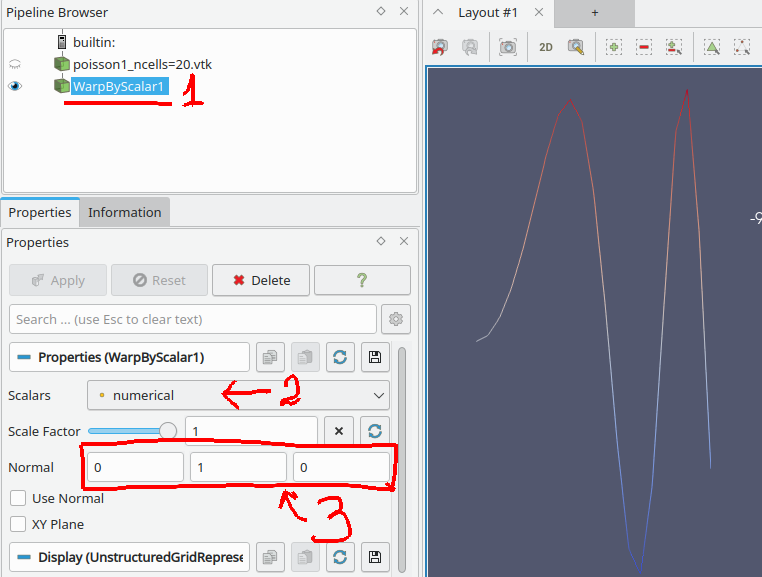
\includegraphics[width=0.5\linewidth]{howto_paraview_1d_3.png}
\end{center}

\paragraph{Цвет и толщина линии}
\begin{enumerate}
\item Включить подробные опции фильтра
\item Сменить стиль на \ename{Solid Color}
\item В меню \ename{Edit} выбрать желаемый цвет
\item В строке \ename{Line Width} указать толщину линии
\end{enumerate}
\begin{center}
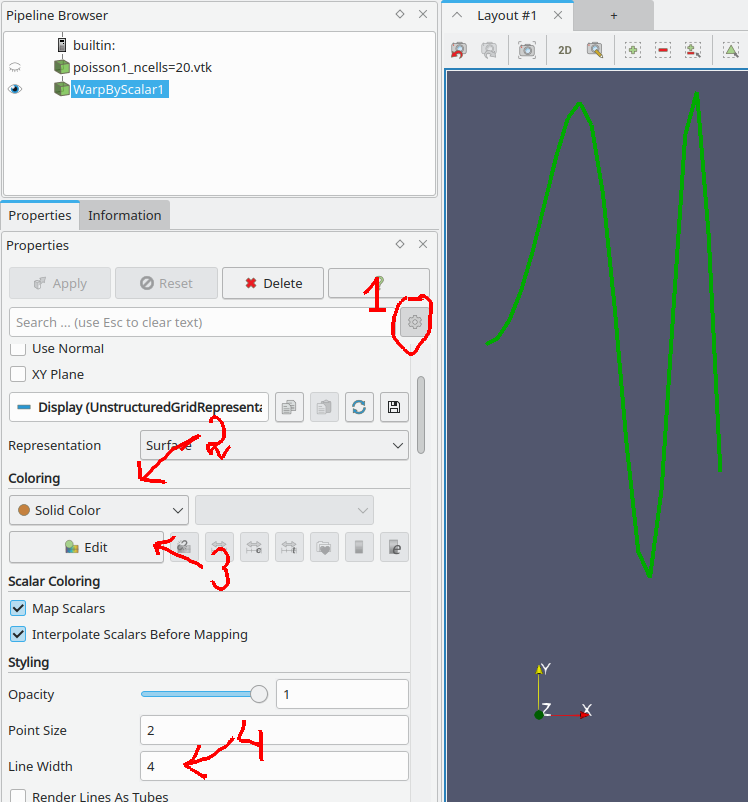
\includegraphics[width=0.6\linewidth]{howto_paraview_1d_4.png}
\end{center}

\paragraph{Настрока масштабов и отображение осей координат}
\begin{enumerate}
\item Отметье подробные настройки фильтра
\item В поле \ename{Transforming/Scale} Установите желаемые масштабы (в нашем случае растянуть в два раза по оси x)
\item Установите галку на отображение осей
\item откройте меню натройки осей
\item В нём включите подробные настроки
\item И также поставьте растяжение осей
\end{enumerate}
В случае, если масштабировать график не нужно, достаточно выполнить шаг 3.
\begin{center}
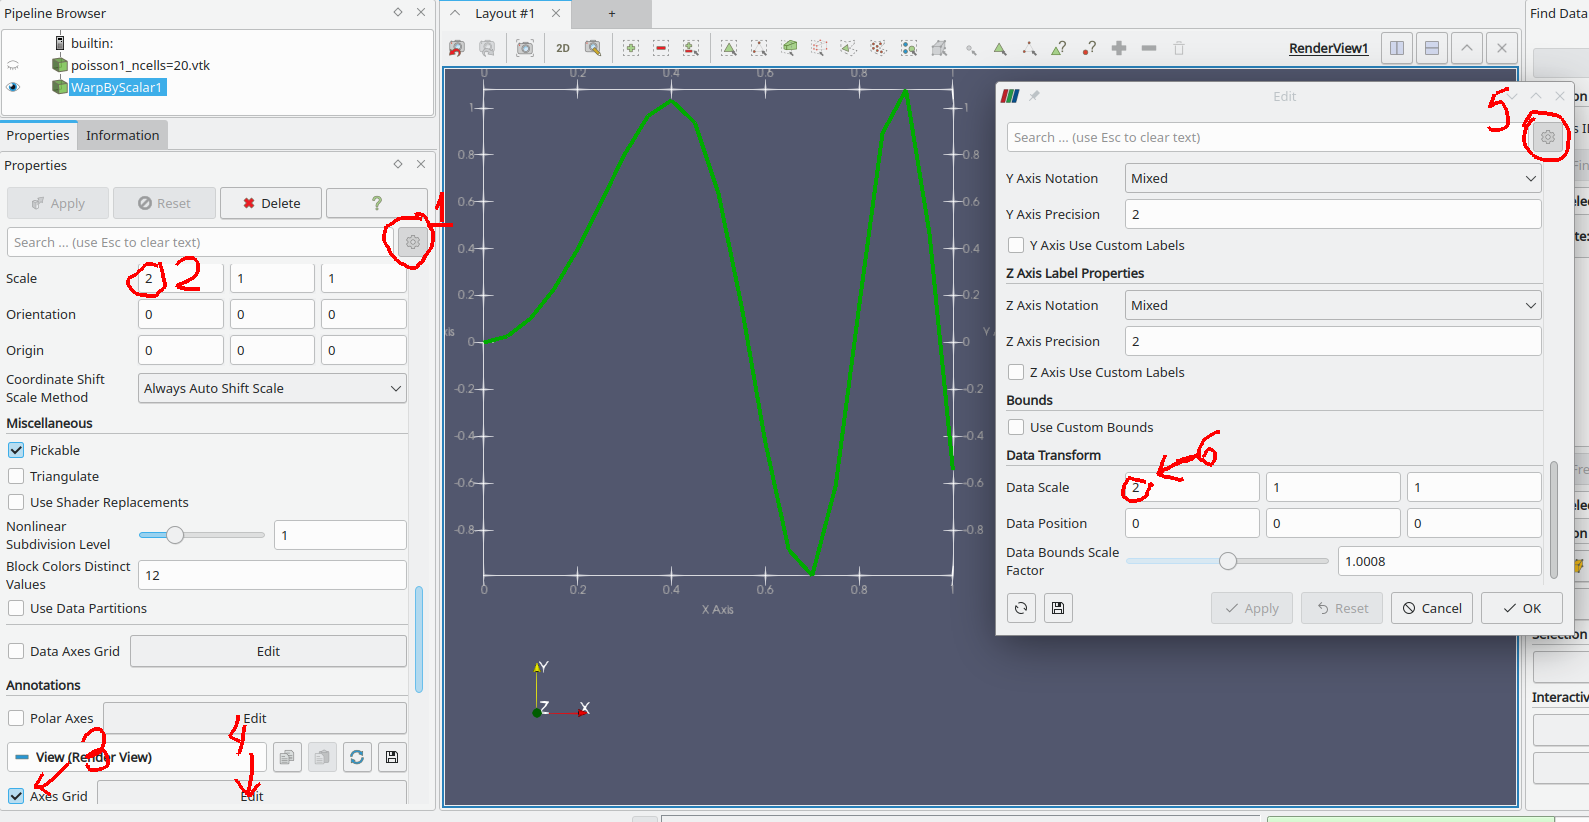
\includegraphics[width=0.9\linewidth]{howto_paraview_1d_5.png}
\end{center}

\paragraph{Построение графиков для нескольких данных}
Если требуется нарисовать рядом несколько графиков для разных данных из одного файла,
примените фильтр \ename{Warp By Scalar} для этого файла ещё раз, изменив поле \ename{Scalars} в настройке фильтра.
Для наглядности измените имя узла в Pipeline Browser на осмысленные
\begin{center}
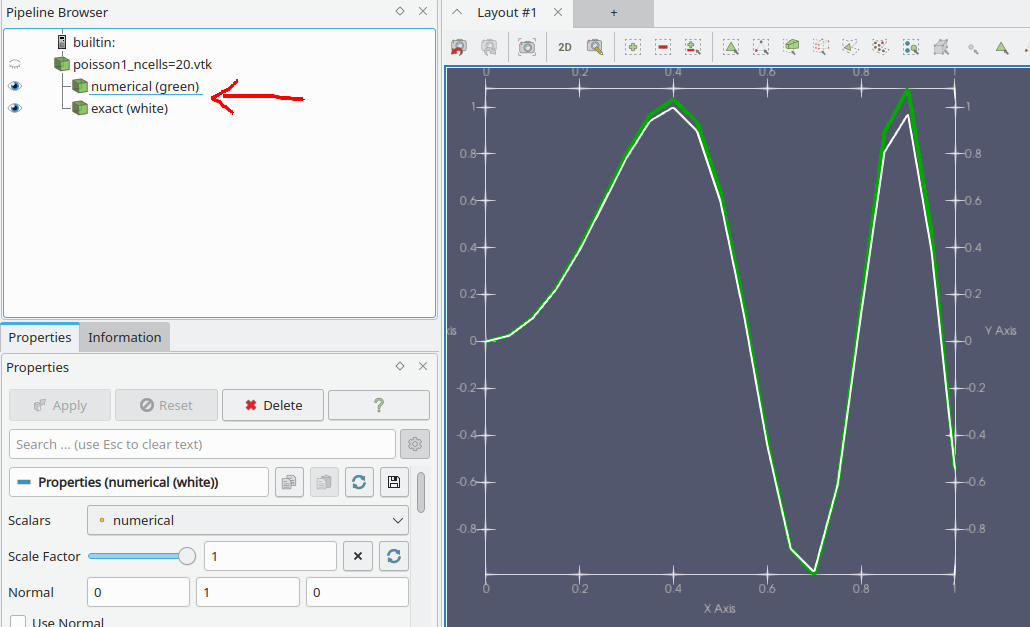
\includegraphics[width=0.8\linewidth]{howto_paraview_1d_6.png}
\end{center}

\paragraph{Обновление данных при изменении исходного файла}
В случае, если исходный файл был изменён, нужно в контекстном меню узла соответствующего файла
выбрать \ename{Reload Files} (или нажать F5). Если те же самые фильтры нужно применить для просмотра другого файла
нужно в этом меню нажать \ename{Change File}.
\begin{center}
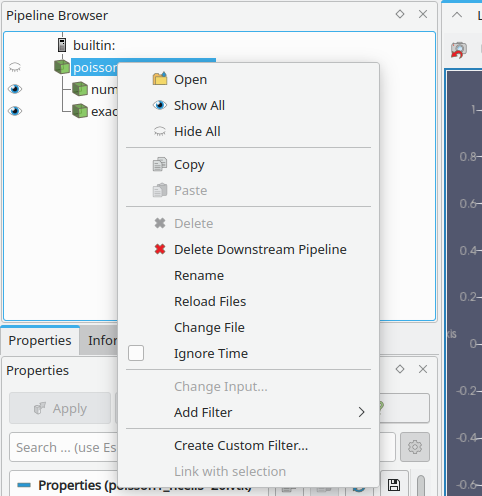
\includegraphics[width=0.4\linewidth]{howto_paraview_1d_7.png}
\end{center}

\subsubsection{Изолинии для двумерного поля}
\label{sec:paraview-isolines}

Ниже представлен алгоритм отрисовки изолиний для данных не сетке,
на которой решение изветно в узлах.
Если вы работаете с данными в ячейках (конечнообъёмная сетка),
следует предварительно применить фильтр \quo{Cell Data To Point Data}.

\begin{enumerate}
\item Нажмите иконку \ename{Contour} (или \ename{Filters/Contour})
      В настройках фильтра Contour by выберитее данные, по которым нужно строить изолинии.
\item В настройках фильтра удалите все существующие записи о значениях для изолиний
\item Добавьте равномерные значения. В появившемся меню установите необходимое количество изолиний и их диапазон.
\item Если необходимо, включите одновременное отображения цветного поля и изолиний.
\end{enumerate}

\begin{center}
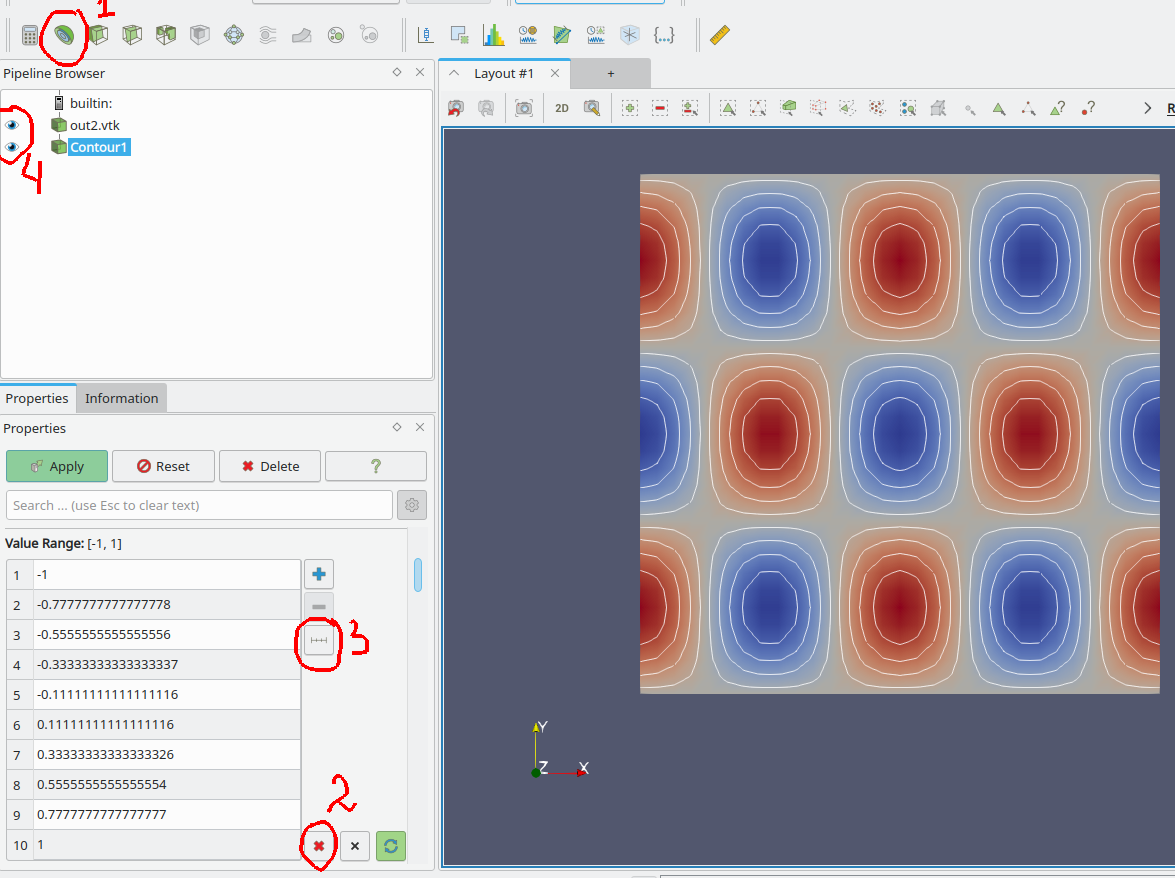
\includegraphics[width=0.7\linewidth]{howto_paraview_isolines_1.png}
\end{center}

\paragraph{Задание цвета и толщины изолинии}
В случае, если нужно сделать изолинии одного цвета, установите поле \ename{Coloring/Solid color} в 
настройках фильтра. Там же в меню \ename{Edit} можно выбрать цвет.
Для установления толщины линии включите подробные настройки и найдите там опцию \ename{Styling/Line Width}.
\begin{center}
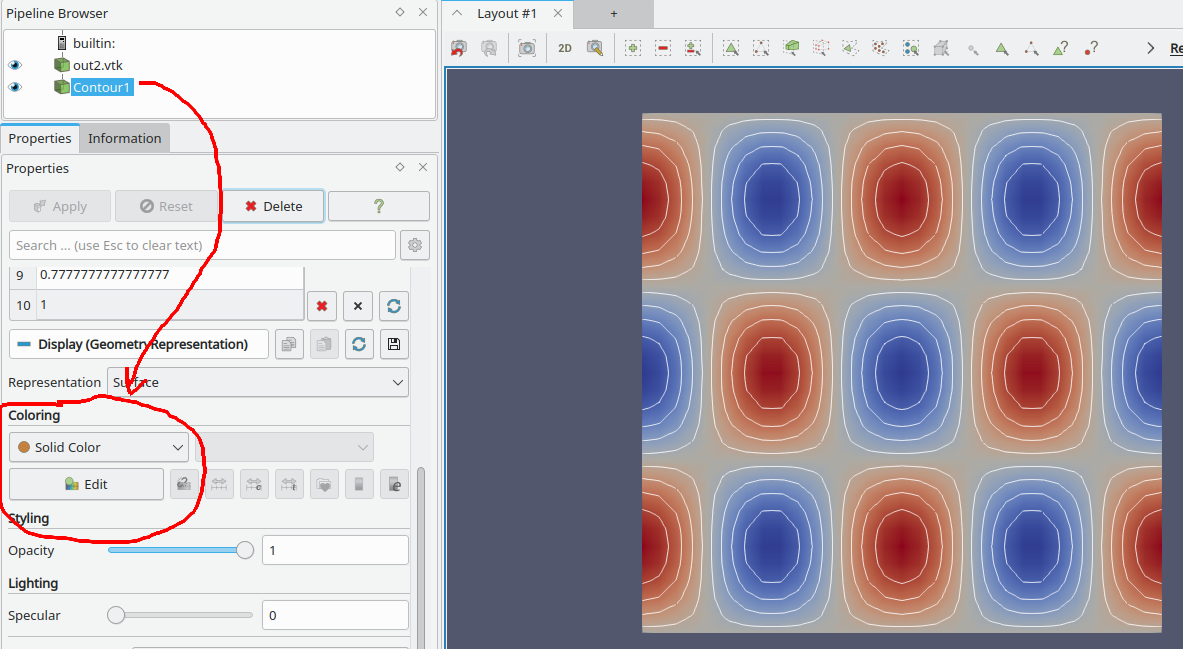
\includegraphics[width=0.7\linewidth]{howto_paraview_isolines_2.png}
\end{center}

\subsubsection{Данные на двумерных сетках в виде поверхности}
\label{sec:paraview-2d}

По аналогии с  одномерным графиком (п.~\ref{sec:paraview-1d}), двумерные поля так же
можно отобразить, проектируя данные на геометрическую координату для получения
объёмного графика. Для этого
\begin{enumerate}
\item Включите фильтр \ename{Filters/Warp By Scalar}
\item В настройках фильтра установите данные, которые будут проектироваться на координату z
\item Установите нормаль для проецирования (ось z)
\item Если нужно, выберите масштабирования для этой координаты
\item После нажатия \ename{Apply} включите трёхмерное отображение
\item Если данные не видно, обновите экран.
\end{enumerate}
\begin{center}
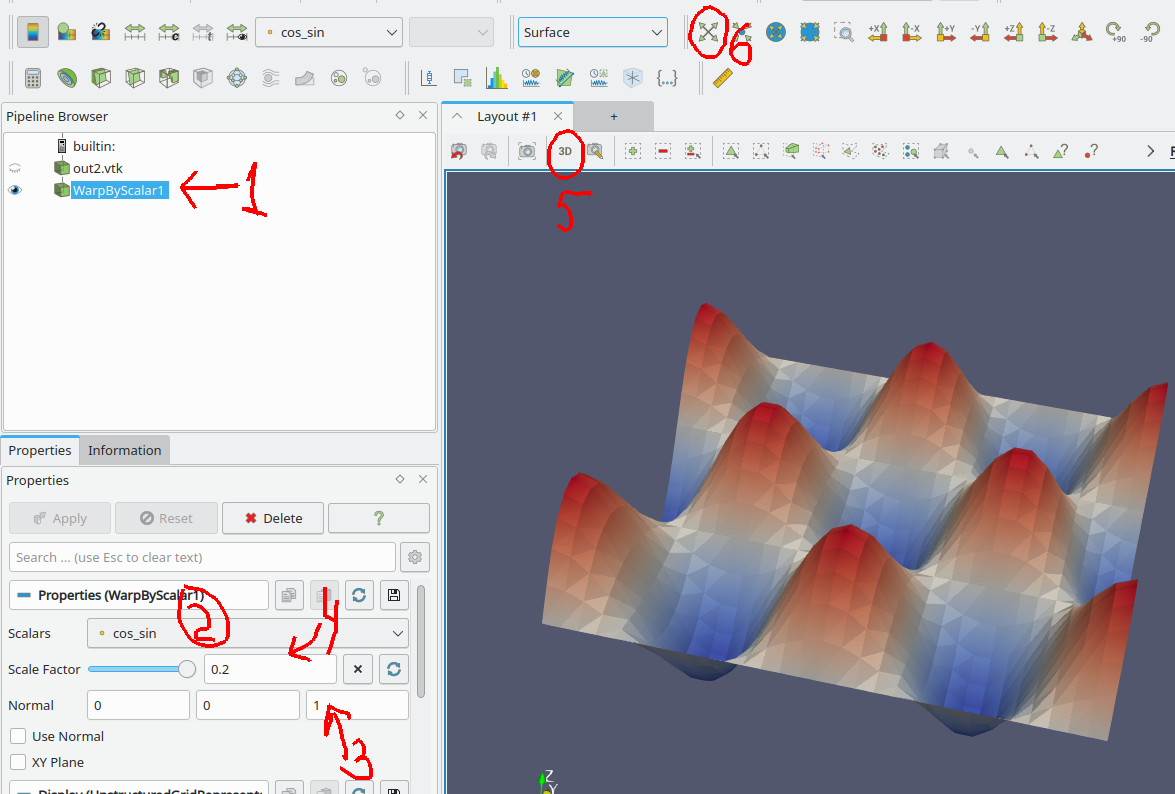
\includegraphics[width=0.9\linewidth]{howto_paraview_2d_as_3d.png}
\end{center}

\subsubsection{Числовых значения в точках и ячейках}
\label{sec:paraview-show-data}

Иногда в процессе отладки или анализа результатов расчёта
требуется знать точное значение поля в заданном узле или ячейке сетки.
Для этого

\begin{enumerate}
\item Включить режим выделения точек или ячеек (иконка (1 на рисунке) или горячие клавиши \ename{s}, \ename{d}).
      Выделить мышкой интересующую область
\item В окне \ename{Find data} (или \ename{Selection Inspector} для старых версий Paraview) отметить поле, которое должно отображаться 
      в центрах ячеек и в точках (2 на рисунке). Если такого окна нет, включить его из основного меню \ename{View}.
\end{enumerate}

\begin{center}
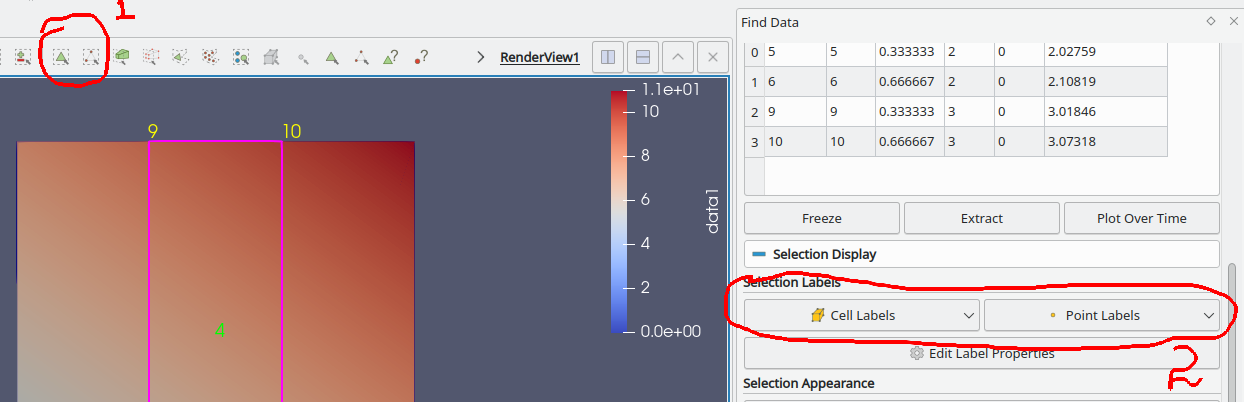
\includegraphics[width=0.8\linewidth]{howto_paraview_show_labels.png}
\end{center}

\subsubsection{Векторные поля}
\label{sec:paraview-glyph}

Открыть файл vtk или vtk.series, который содержит
векторное поле. Далее
\begin{enumerate}
\item Создать фильтр \ename{Glyph}
\item Задать двумерный тип стрелки
\item Сместить центр стрелки, чтобы она исходила из точки, к которой приписана
\item Отметить необходимое векторное поле в качестве ориентации
\item Отметить необходимое векторное поле для масштабирования
      Нажать \ename{Apply}.
\end{enumerate}

\begin{center}
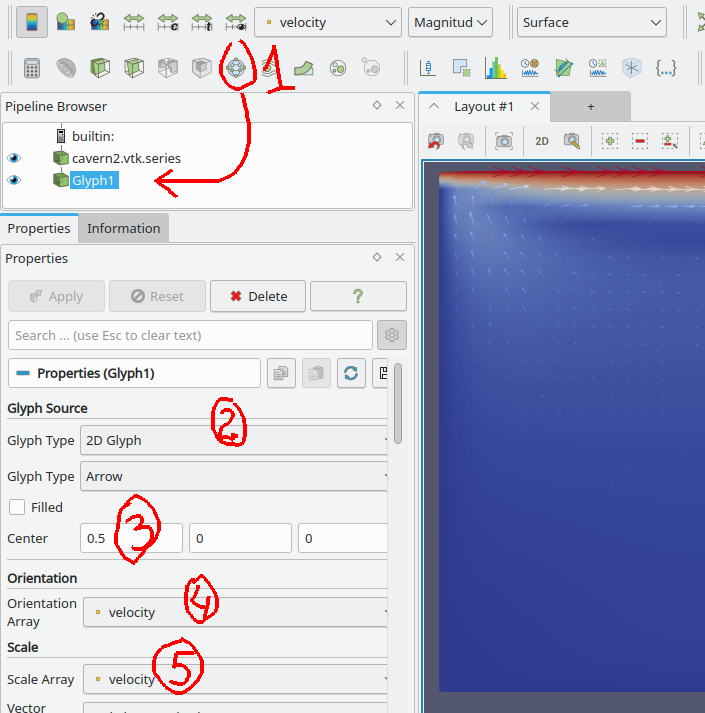
\includegraphics[width=0.6\linewidth]{glyph-1.png}
\end{center}

\paragraph{Настройка отображения стрелок}
\begin{enumerate}
\item Выбрать необходимый \ename{Glyph-mode}. Если сетка небольшая, то можно \ename{All Points}.
\item Установить белый цвет для стрелок. Нажать Apply.
\end{enumerate}

\begin{center}
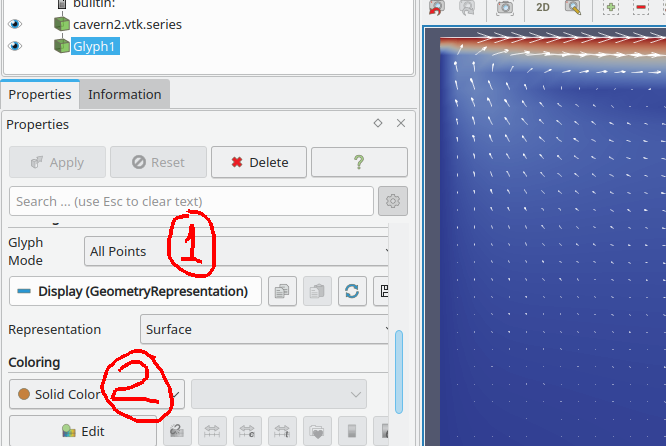
\includegraphics[width=0.4\linewidth]{glyph-2.png}
\end{center}

\paragraph{Уменьшения разброса по длине стрелок}
Если разброс по длинам стрелок слишком велик, его можно подравнять,
введя новую функцию $|\vec v|^{\alpha}$ -- длина вектора в степени меньше единицы (например, $\alpha=0.7$).
Такую функцию можно создать через калькулятор

\begin{enumerate}
\item Начиная от загруженного файла создать фильтр \ename{Calculator}
\item Там вбить необходимую формулу
\end{enumerate}
\begin{center}
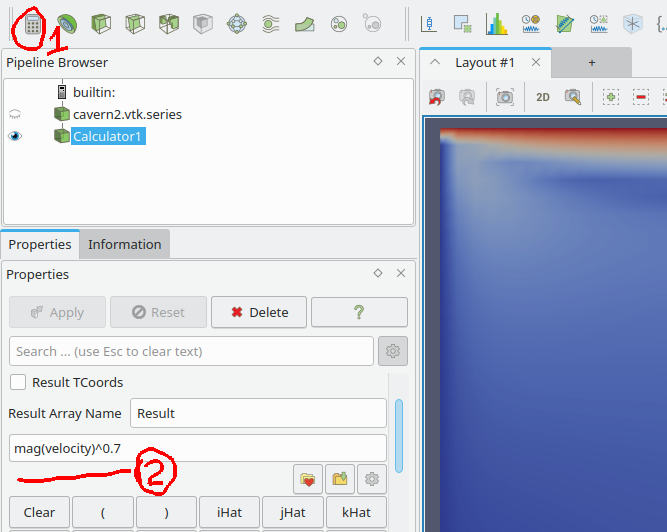
\includegraphics[width=0.6\linewidth]{glyph-3.png}
\end{center}
Созданную функцию нужно прокинуть в \ename{Glyph} в качестве коэффициента масштабирования
\begin{enumerate}
\item В \ename{Scale Array} фильтра \ename{Glyph} указать уже результат работы \ename{Calculator}-a (\ename{Result} по умолчанию),
\item Подтянуть значение \ename{Scale Factor} до приемлимого
\item Не забыть отключить вспомогательное поле \ename{Calculator} из отображения
\end{enumerate}
\begin{center}
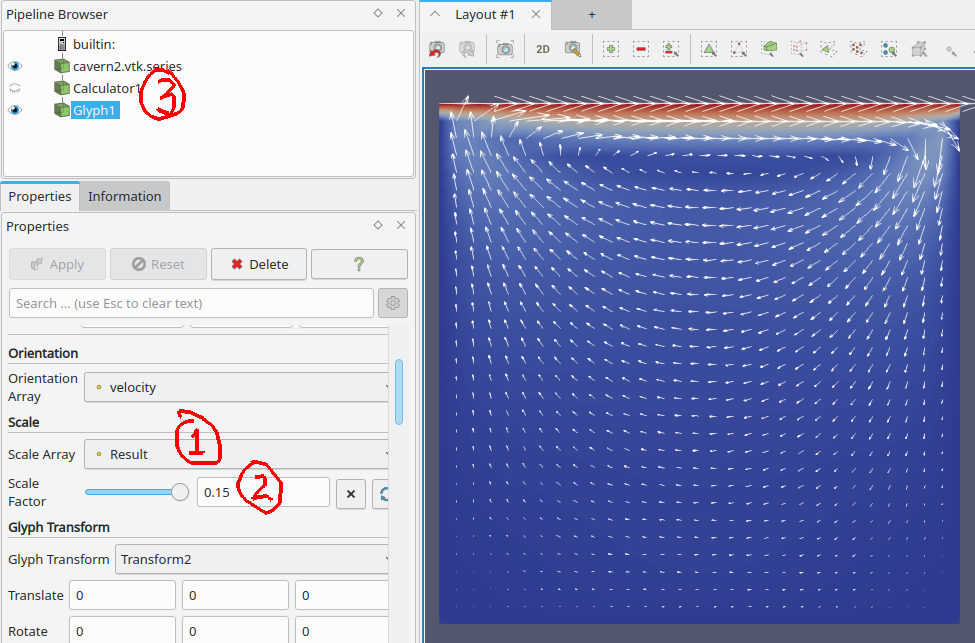
\includegraphics[width=0.6\linewidth]{glyph-4.png}
\end{center}

\subsubsection{Значение функции вдоль линии}
\label{sec:paraview-plot-over-line}

\begin{enumerate}
\item
Выбрать фильтр \ename{Plot Over Line} иконкой или в меню \ename{Filters}
\item
Установить начальную и конечную точку сечения
\item
Можно использовать привязку к узлам сетки с помощью горячих клавиш (в подсказках написано)
\item
Можно установить координаты руками в соответствующем поле. Для двумерных задач проследить,
что координата Z равна нулю
\item
Нажать \ename{Apply}
\end{enumerate}

\begin{center}
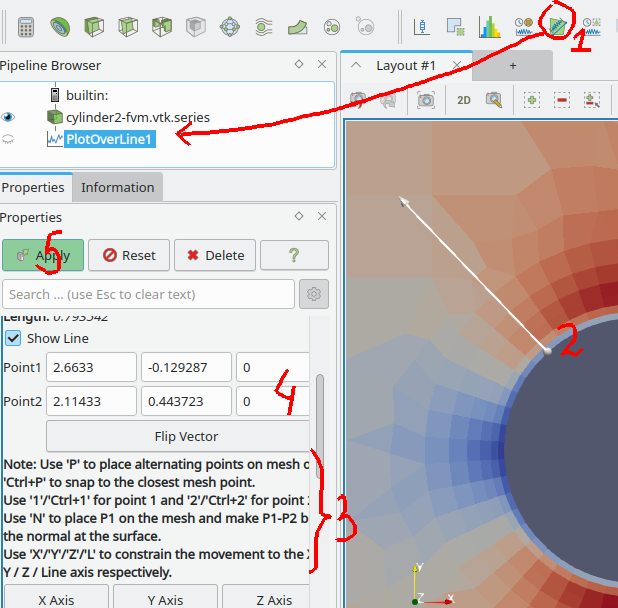
\includegraphics[width=0.4\linewidth]{howto_paraview_plot_over_line_1.png}
\end{center}

\paragraph{Настройка графика}
\begin{enumerate}
\item
После установок появится дополнительное окно типа \ename{Line Chart View} с нарисованным графиком.
\item
Сделав это окно активным в настройках фильтра \ename{PlotOverLine}
можно выбрать, какие поля рисовать (\ename{Series Parameters})
\end{enumerate}

\begin{center}
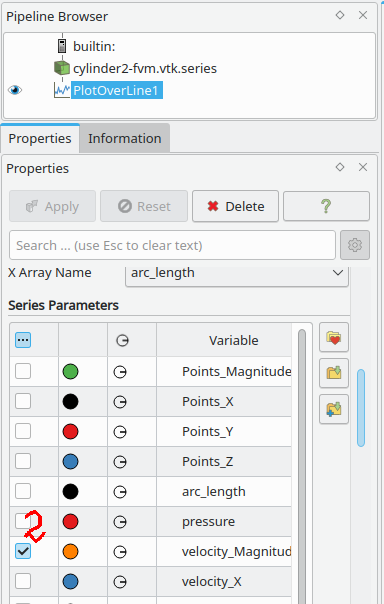
\includegraphics[width=0.2\linewidth]{howto_paraview_plot_over_line_3.png}
\quad
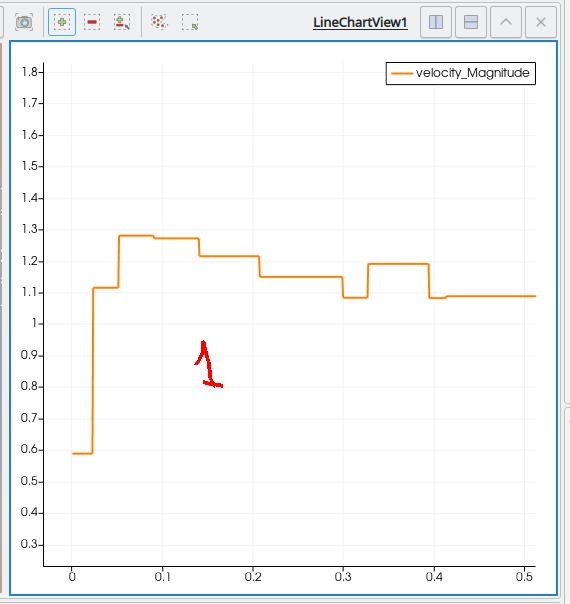
\includegraphics[width=0.3\linewidth]{howto_paraview_plot_over_line_2.png}
\end{center}

\paragraph{Отрисовка в отдельном окне}
\begin{enumerate}
\item
Открыть новую вкладку
\item
Выбрать \ename{Line Chart View}
\item
Выбрать предварительно созданный фильтр с одномерным графиком
\end{enumerate}
\begin{center}
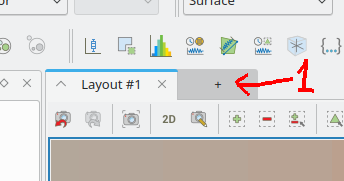
\includegraphics[width=0.2\linewidth]{howto_paraview_plot_over_line_4.png}
\quad
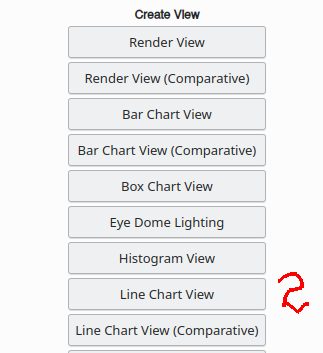
\includegraphics[width=0.3\linewidth]{howto_paraview_plot_over_line_5.png}
\quad
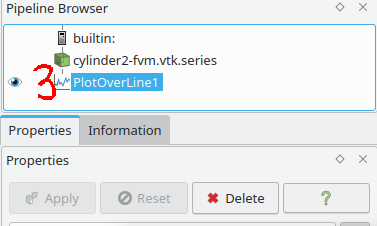
\includegraphics[width=0.3\linewidth]{howto_paraview_plot_over_line_6.png}
\end{center}

\subsection{Hybmesh}
\label{sec:hybmesh}

Генератор сеток на основе композитного подхода.
Работает на основе python-скрипотов.
Полная документация \url{http://kalininei.github.io/HybMesh/index.html}

\subsubsection{Построение сеток}
Скрипты построения сетки лежат в папке \ename{/app/test-data}.
Для запуска скрипта построения сетки следует находясь в контейнере перейти в эту папку
и запустить (например для \ename{trigrid.py})
\begin{shelloutput}
cd /app/test-data
hybmesh -sx trigrid.py
\end{shelloutput}

При первом запуске система предложит собрать и установить hybmesh из исходников.
Следует согласиться, введя \cvar{y}. Первое построение может занять несколько минут.

\subsection{Приёмы отладки}
\label{sec:debug}
\subsubsection{Печать разреженной матрицы}
\label{sec:dbg-print-csr}
Для вывода разреженных матриц любого формата
(реализующего интерфейс \cvar{ISparseMatrix})
Можно воспользоваться функцией \cvar{dbg::print}
(её можно вызывать непосредственно в процессе отладки
не прерываясь на расстановку нужных вызовов в коде и перекомпиляцию).
\begin{cppcode}
#include "cfd/debug/printer.hpp"
...

LodMatrix M(3);
M.add_value(0, 0, 1.0); 
M.add_value(1, 0, 0.0); 
M.add_value(1, 1, 4.0); 
M.add_value(2, 2, 3.0); 
dbg::print(M);
\end{cppcode}
В результате в терминал выведется матрица
\begin{shelloutput}
-- SIZE = 3x3
     1      *      *
     0      4      *
     *      *      3
\end{shelloutput}
Здесь \cvar{*} -- отмечены места, где отсутсвует значение в шаблоне матрицы (то есть ноль по построению).
Заданные в шаблоне значения тоже могут быть нулями (как в настоящем примере на второй строке первой колонки).

Если матрица имеет большую размерность, то печатать всю матрицу целиком неудобно.
Но можно воспользоваться печатью отдельной строки.
Так вызов
\begin{cppcode}
dbg::print(1, M);
\end{cppcode}
выведет только значения второй строки матрицы, находящиеся в шаблоне
\begin{shelloutput}
-- ROW = 1
   [   0] 0   // M[1, 0] = 0
   [   1] 4   // M[1, 1] = 4
\end{shelloutput}

\subsubsection{Сохранение отладочных полей решения}
В процессе отладки работы с сеточными данными
часто возникает необходимость быстро отобразить
их на сетке. Для этого в файле \ename{debug/saver.hpp}
имеется набор вспомогательных функций (каждая из них может быть запущена непоследственно из отладчика):

\begin{cppcode}
// скаляр в узлах сетки
void save_point_data(const IGrid& grid, const std::vector<double>& data);
// скаляр в ячейках сетки
void save_cell_data(const IGrid& grid, const std::vector<double>& data);
// вектор в ячейках сетки
void save_cell_vector(const IGrid& grid, const std::vector<Vector>& vec);
// скаляр в расширенных точках коллокации (ячейки + граничные грани)
void save_extended_colloc_data(const IGrid& grid, const std::vector<double>& data);
// скаляр в гранях сетки
void save_face_data(const IGrid& grid, const std::vector<double>& data);
\end{cppcode}

Все эти функции сохраняют данные в файл \ename{dbg.vtk} в текущую папку из которой запущена программа.

\subsubsection{Профилирование}
\label{sec:dbg-tictoc}
Для профилирования (замера время исполнения участков кода) можно пользоваться
набором глобальных функций, определённых в файле
\ename{debug/tictoc.hpp}.

\paragraph{Простой замер времени}
Измерение времени исполнения участка кода:
\begin{cppcode}
#include "cfd/debug/tictoc.hpp"
...

dbg::Tic("process1");   // начать замер (блок с именем process1)
// ... код, время исполнение которого требуется замерить
std::this_thread::sleep_for(std::chrono::milliseconds(40));
dbg::Toc("process1");   // окончить замер
\end{cppcode}

По окончанию работы программы в терминал будет распечатан
отчёт о времени исполнения каждого блока (в миллисекундах)
\begin{shelloutput}
------ Tictoc report (ms)
Process        Total time    Calls count  Time per call
-------------------------------------------------------
process1               40              1             40
\end{shelloutput}

Названия секций может быть произвольным и может повторяться. В последнем случае
программа будет выводить как общее время исполнение этого блока, так и среднее время по запускам:

\begin{cppcode}
dbg::Tic("process1");
std::this_thread::sleep_for(std::chrono::milliseconds(40));
dbg::Toc("process1");

dbg::Tic("process1");
std::this_thread::sleep_for(std::chrono::milliseconds(50));
dbg::Toc("process1");
\end{cppcode}

\begin{shelloutput}
------ Tictoc report (ms)
Process        Total time    Calls count  Time per call
-------------------------------------------------------
process1               90              2             45
\end{shelloutput}

\paragraph{Замер времени внутри области видимости}
Чтобы не писать \cvar{Toc} для остановки таймера
можно использовать замер внутри текущей области видимомости (внутри текущих фигурных скобок) используя
метод \cvar{ScopedTic}.
Например, чтобы замерить время работы метода можно написать
\begin{cppcode}
void heavy_func(){
    auto tic = dbg::ScopedTic("heavy_func");
    std::this_thread::sleep_for(std::chrono::milliseconds(50));

    // объект tic удалится при выходы из области видимости
    // и таймер для процесса heavy_func будет остановлен
}
\end{cppcode}

\paragraph{Индексированные процессы}
Иногда бывает полезно разбить один процесс
на несколько подпроцессов. Для этого можно воспользоваться индексированными
именами. В отчёт при этом
пойдет как время исполнения каждого шага процесса, так и общее время.
\begin{cppcode}
{
    auto tic = dbg::ScopedTic("process", 1);
    std::this_thread::sleep_for(std::chrono::milliseconds(50));
}
{
    auto tic = dbg::ScopedTic("process", 2);
    std::this_thread::sleep_for(std::chrono::milliseconds(20));
}
{
    auto tic = dbg::ScopedTic("process", 3);
    std::this_thread::sleep_for(std::chrono::milliseconds(10));
}
\end{cppcode}
\begin{shelloutput}
------ Tictoc report (ms)
Process        Total time    Calls count  Time per call
-------------------------------------------------------
process                80              3             26
process-1              50              1             50
process-2              20              1             20
process-3              10              1             10
\end{shelloutput}

Это механизм удобно использовать для замера
времени исполнения тела цикла (если кол-во итераций небольшое)
\begin{cppcode}
for (size_t i=0; i<3; ++i){
    dbg::Tic("loop", i);
    std::this_thread::sleep_for(std::chrono::milliseconds(50-i));
    dbg::Toc("loop", i);
}
\end{cppcode}

\paragraph{Печать отчётов}
По умолчанию программа печатает
финальный отчёт о выполнении по окончании
работы программы.
Если требуется распечатать отчёт раньше, можно
явно вызывать метод \cvar{dbg::Report} или
\cvar{dbg::FinReport}.
Последний обнуляет все таймеры и может быть удобен
при запуске нескольких расчётов с разными параметрами:
\begin{cppcode}
for (size_t n_cells: {10, 20, 50}){
    calculate(n_cells);
    FinReport();  // печать отчёта о профилировании только для текущего расчёта
}
\end{cppcode}


\end{document}
